% Options for packages loaded elsewhere
\PassOptionsToPackage{unicode}{hyperref}
\PassOptionsToPackage{hyphens}{url}
\PassOptionsToPackage{dvipsnames,svgnames,x11names}{xcolor}
%
\documentclass[
  letterpaper,
  DIV=11,
  numbers=noendperiod]{scrreprt}

\usepackage{amsmath,amssymb}
\usepackage{iftex}
\ifPDFTeX
  \usepackage[T1]{fontenc}
  \usepackage[utf8]{inputenc}
  \usepackage{textcomp} % provide euro and other symbols
\else % if luatex or xetex
  \usepackage{unicode-math}
  \defaultfontfeatures{Scale=MatchLowercase}
  \defaultfontfeatures[\rmfamily]{Ligatures=TeX,Scale=1}
\fi
\usepackage{lmodern}
\ifPDFTeX\else  
    % xetex/luatex font selection
\fi
% Use upquote if available, for straight quotes in verbatim environments
\IfFileExists{upquote.sty}{\usepackage{upquote}}{}
\IfFileExists{microtype.sty}{% use microtype if available
  \usepackage[]{microtype}
  \UseMicrotypeSet[protrusion]{basicmath} % disable protrusion for tt fonts
}{}
\makeatletter
\@ifundefined{KOMAClassName}{% if non-KOMA class
  \IfFileExists{parskip.sty}{%
    \usepackage{parskip}
  }{% else
    \setlength{\parindent}{0pt}
    \setlength{\parskip}{6pt plus 2pt minus 1pt}}
}{% if KOMA class
  \KOMAoptions{parskip=half}}
\makeatother
\usepackage{xcolor}
\setlength{\emergencystretch}{3em} % prevent overfull lines
\setcounter{secnumdepth}{5}
% Make \paragraph and \subparagraph free-standing
\ifx\paragraph\undefined\else
  \let\oldparagraph\paragraph
  \renewcommand{\paragraph}[1]{\oldparagraph{#1}\mbox{}}
\fi
\ifx\subparagraph\undefined\else
  \let\oldsubparagraph\subparagraph
  \renewcommand{\subparagraph}[1]{\oldsubparagraph{#1}\mbox{}}
\fi

\usepackage{color}
\usepackage{fancyvrb}
\newcommand{\VerbBar}{|}
\newcommand{\VERB}{\Verb[commandchars=\\\{\}]}
\DefineVerbatimEnvironment{Highlighting}{Verbatim}{commandchars=\\\{\}}
% Add ',fontsize=\small' for more characters per line
\usepackage{framed}
\definecolor{shadecolor}{RGB}{241,243,245}
\newenvironment{Shaded}{\begin{snugshade}}{\end{snugshade}}
\newcommand{\AlertTok}[1]{\textcolor[rgb]{0.68,0.00,0.00}{#1}}
\newcommand{\AnnotationTok}[1]{\textcolor[rgb]{0.37,0.37,0.37}{#1}}
\newcommand{\AttributeTok}[1]{\textcolor[rgb]{0.40,0.45,0.13}{#1}}
\newcommand{\BaseNTok}[1]{\textcolor[rgb]{0.68,0.00,0.00}{#1}}
\newcommand{\BuiltInTok}[1]{\textcolor[rgb]{0.00,0.23,0.31}{#1}}
\newcommand{\CharTok}[1]{\textcolor[rgb]{0.13,0.47,0.30}{#1}}
\newcommand{\CommentTok}[1]{\textcolor[rgb]{0.37,0.37,0.37}{#1}}
\newcommand{\CommentVarTok}[1]{\textcolor[rgb]{0.37,0.37,0.37}{\textit{#1}}}
\newcommand{\ConstantTok}[1]{\textcolor[rgb]{0.56,0.35,0.01}{#1}}
\newcommand{\ControlFlowTok}[1]{\textcolor[rgb]{0.00,0.23,0.31}{#1}}
\newcommand{\DataTypeTok}[1]{\textcolor[rgb]{0.68,0.00,0.00}{#1}}
\newcommand{\DecValTok}[1]{\textcolor[rgb]{0.68,0.00,0.00}{#1}}
\newcommand{\DocumentationTok}[1]{\textcolor[rgb]{0.37,0.37,0.37}{\textit{#1}}}
\newcommand{\ErrorTok}[1]{\textcolor[rgb]{0.68,0.00,0.00}{#1}}
\newcommand{\ExtensionTok}[1]{\textcolor[rgb]{0.00,0.23,0.31}{#1}}
\newcommand{\FloatTok}[1]{\textcolor[rgb]{0.68,0.00,0.00}{#1}}
\newcommand{\FunctionTok}[1]{\textcolor[rgb]{0.28,0.35,0.67}{#1}}
\newcommand{\ImportTok}[1]{\textcolor[rgb]{0.00,0.46,0.62}{#1}}
\newcommand{\InformationTok}[1]{\textcolor[rgb]{0.37,0.37,0.37}{#1}}
\newcommand{\KeywordTok}[1]{\textcolor[rgb]{0.00,0.23,0.31}{#1}}
\newcommand{\NormalTok}[1]{\textcolor[rgb]{0.00,0.23,0.31}{#1}}
\newcommand{\OperatorTok}[1]{\textcolor[rgb]{0.37,0.37,0.37}{#1}}
\newcommand{\OtherTok}[1]{\textcolor[rgb]{0.00,0.23,0.31}{#1}}
\newcommand{\PreprocessorTok}[1]{\textcolor[rgb]{0.68,0.00,0.00}{#1}}
\newcommand{\RegionMarkerTok}[1]{\textcolor[rgb]{0.00,0.23,0.31}{#1}}
\newcommand{\SpecialCharTok}[1]{\textcolor[rgb]{0.37,0.37,0.37}{#1}}
\newcommand{\SpecialStringTok}[1]{\textcolor[rgb]{0.13,0.47,0.30}{#1}}
\newcommand{\StringTok}[1]{\textcolor[rgb]{0.13,0.47,0.30}{#1}}
\newcommand{\VariableTok}[1]{\textcolor[rgb]{0.07,0.07,0.07}{#1}}
\newcommand{\VerbatimStringTok}[1]{\textcolor[rgb]{0.13,0.47,0.30}{#1}}
\newcommand{\WarningTok}[1]{\textcolor[rgb]{0.37,0.37,0.37}{\textit{#1}}}

\providecommand{\tightlist}{%
  \setlength{\itemsep}{0pt}\setlength{\parskip}{0pt}}\usepackage{longtable,booktabs,array}
\usepackage{calc} % for calculating minipage widths
% Correct order of tables after \paragraph or \subparagraph
\usepackage{etoolbox}
\makeatletter
\patchcmd\longtable{\par}{\if@noskipsec\mbox{}\fi\par}{}{}
\makeatother
% Allow footnotes in longtable head/foot
\IfFileExists{footnotehyper.sty}{\usepackage{footnotehyper}}{\usepackage{footnote}}
\makesavenoteenv{longtable}
\usepackage{graphicx}
\makeatletter
\def\maxwidth{\ifdim\Gin@nat@width>\linewidth\linewidth\else\Gin@nat@width\fi}
\def\maxheight{\ifdim\Gin@nat@height>\textheight\textheight\else\Gin@nat@height\fi}
\makeatother
% Scale images if necessary, so that they will not overflow the page
% margins by default, and it is still possible to overwrite the defaults
% using explicit options in \includegraphics[width, height, ...]{}
\setkeys{Gin}{width=\maxwidth,height=\maxheight,keepaspectratio}
% Set default figure placement to htbp
\makeatletter
\def\fps@figure{htbp}
\makeatother

\KOMAoption{captions}{tableheading}
\makeatletter
\@ifpackageloaded{tcolorbox}{}{\usepackage[skins,breakable]{tcolorbox}}
\@ifpackageloaded{fontawesome5}{}{\usepackage{fontawesome5}}
\definecolor{quarto-callout-color}{HTML}{909090}
\definecolor{quarto-callout-note-color}{HTML}{0758E5}
\definecolor{quarto-callout-important-color}{HTML}{CC1914}
\definecolor{quarto-callout-warning-color}{HTML}{EB9113}
\definecolor{quarto-callout-tip-color}{HTML}{00A047}
\definecolor{quarto-callout-caution-color}{HTML}{FC5300}
\definecolor{quarto-callout-color-frame}{HTML}{acacac}
\definecolor{quarto-callout-note-color-frame}{HTML}{4582ec}
\definecolor{quarto-callout-important-color-frame}{HTML}{d9534f}
\definecolor{quarto-callout-warning-color-frame}{HTML}{f0ad4e}
\definecolor{quarto-callout-tip-color-frame}{HTML}{02b875}
\definecolor{quarto-callout-caution-color-frame}{HTML}{fd7e14}
\makeatother
\makeatletter
\makeatother
\makeatletter
\@ifpackageloaded{bookmark}{}{\usepackage{bookmark}}
\makeatother
\makeatletter
\@ifpackageloaded{caption}{}{\usepackage{caption}}
\AtBeginDocument{%
\ifdefined\contentsname
  \renewcommand*\contentsname{Table of contents}
\else
  \newcommand\contentsname{Table of contents}
\fi
\ifdefined\listfigurename
  \renewcommand*\listfigurename{List of Figures}
\else
  \newcommand\listfigurename{List of Figures}
\fi
\ifdefined\listtablename
  \renewcommand*\listtablename{List of Tables}
\else
  \newcommand\listtablename{List of Tables}
\fi
\ifdefined\figurename
  \renewcommand*\figurename{Figure}
\else
  \newcommand\figurename{Figure}
\fi
\ifdefined\tablename
  \renewcommand*\tablename{Table}
\else
  \newcommand\tablename{Table}
\fi
}
\@ifpackageloaded{float}{}{\usepackage{float}}
\floatstyle{ruled}
\@ifundefined{c@chapter}{\newfloat{codelisting}{h}{lop}}{\newfloat{codelisting}{h}{lop}[chapter]}
\floatname{codelisting}{Listing}
\newcommand*\listoflistings{\listof{codelisting}{List of Listings}}
\makeatother
\makeatletter
\@ifpackageloaded{caption}{}{\usepackage{caption}}
\@ifpackageloaded{subcaption}{}{\usepackage{subcaption}}
\makeatother
\makeatletter
\@ifpackageloaded{tcolorbox}{}{\usepackage[skins,breakable]{tcolorbox}}
\makeatother
\makeatletter
\@ifundefined{shadecolor}{\definecolor{shadecolor}{rgb}{.97, .97, .97}}
\makeatother
\makeatletter
\makeatother
\makeatletter
\makeatother
\ifLuaTeX
  \usepackage{selnolig}  % disable illegal ligatures
\fi
\IfFileExists{bookmark.sty}{\usepackage{bookmark}}{\usepackage{hyperref}}
\IfFileExists{xurl.sty}{\usepackage{xurl}}{} % add URL line breaks if available
\urlstyle{same} % disable monospaced font for URLs
\hypersetup{
  pdftitle={Computer Vision},
  pdfauthor={Bengkel Koding},
  colorlinks=true,
  linkcolor={blue},
  filecolor={Maroon},
  citecolor={Blue},
  urlcolor={Blue},
  pdfcreator={LaTeX via pandoc}}

\title{Computer Vision}
\author{Bengkel Koding}
\date{2023-07-28}

\begin{document}
\maketitle
\ifdefined\Shaded\renewenvironment{Shaded}{\begin{tcolorbox}[breakable, enhanced, borderline west={3pt}{0pt}{shadecolor}, frame hidden, boxrule=0pt, interior hidden, sharp corners]}{\end{tcolorbox}}\fi

\renewcommand*\contentsname{Table of contents}
{
\hypersetup{linkcolor=}
\setcounter{tocdepth}{2}
\tableofcontents
}
\bookmarksetup{startatroot}

\hypertarget{pengantar}{%
\chapter*{\texorpdfstring{\textbf{Pengantar}}{Pengantar}}\label{pengantar}}
\addcontentsline{toc}{chapter}{\textbf{Pengantar}}

\markboth{\textbf{Pengantar}}{\textbf{Pengantar}}

\hypertarget{tentang-kursus-ini}{%
\section*{Tentang Kursus ini}\label{tentang-kursus-ini}}
\addcontentsline{toc}{section}{Tentang Kursus ini}

\markright{Tentang Kursus ini}

Kursus ini dirancang sebagai panduan komprehensif untuk memahami dan
menerapkan teknik computer vision menggunakan bahasa pemrograman Python.
Kursus ini ditujukan untuk individu yang berminat dalam bidang computer
vision, baik mereka yang baru memulai perjalanan mereka atau mereka yang
sudah memiliki pengalaman dasar dalam bidang ini dan ingin memperdalam
pengetahuan mereka.

Kursus ini mencakup berbagai topik mulai dari konsep dasar computer
vision dan image processing, hingga teknik machine learning dan deep
learning yang canggih yang digunakan dalam aplikasi computer vision.
Selain itu, kursus ini juga mencakup bagian penting tentang etika dalam
computer vision, suatu topik yang sering diabaikan tetapi sangat
penting.

Dalam kursus ini, pembaca akan belajar melalui penjelasan konsep, contoh
kode, gambar, diagram, latihan, dan proyek praktis. Tujuan utama kursus
ini adalah untuk memberikan pemahaman yang solid tentang konsep dasar
dan lanjutan dalam computer vision dan bagaimana menerapkannya dalam
situasi dunia nyata menggunakan Python.

\part{ Konsep }

\hypertarget{pengenalan-kursus-computer-vision-dan-python}{%
\section*{Pengenalan Kursus Computer Vision dan
Python}\label{pengenalan-kursus-computer-vision-dan-python}}
\addcontentsline{toc}{section}{Pengenalan Kursus Computer Vision dan
Python}

\markright{Pengenalan Kursus Computer Vision dan Python}

Kursus ini bertujuan untuk memperkenalkan Anda pada konsep dan praktik
Computer Vision menggunakan Python. Selama kursus ini, Anda akan
mempelajari dasar-dasar Computer Vision dan mengapa Python menjadi
bahasa pemrograman yang populer dalam bidang ini.

Hal yang akan dipelajari dalam kursus ini meliputi:

\textbf{Module 1}: Pengenalan Computer Vision dan Python Pada modul ini,
kita akan mempelajari pengenalan dasar tentang Computer Vision dan
Python. Kami akan memahami definisi dan sejarah Computer Vision, serta
aplikasi dan contoh penggunaannya dalam kehidupan sehari-hari. Kami juga
akan membahas perbedaan antara Computer Vision dan Image Processing.
Selain itu, Anda akan diperkenalkan dengan Python, termasuk sejarah,
keunggulan, cara instalasi, dan struktur bahasa pemrograman Python. Kami
akan memperkenalkan beberapa library Python yang umum digunakan dalam
Computer Vision, seperti OpenCV, TensorFlow, dan Keras, dan cara
menginstal dan menggunakannya.

\textbf{Module 2}: Dasar-dasar Image Processing Pada modul ini, kami
akan membahas dasar-dasar Image Processing. Anda akan mempelajari
definisi dan sejarah Image Processing, serta aplikasi dan contoh
penggunaannya. Kami akan memperkenalkan konsep dasar dalam pemrosesan
citra, termasuk pengenalan citra digital dan operasi dasar pada citra
seperti transformasi, filtering, dan edge detection. Anda juga akan
belajar tentang penggunaan library Python seperti OpenCV, PIL/Pillow,
dan scikit-image untuk operasi dasar pemrosesan citra. Modul ini akan
mencakup latihan praktik untuk menerapkan operasi dasar tersebut pada
dataset gambar menggunakan Python.

\textbf{Module 3}: Feature Extraction and Matching Modul ini akan
membahas tentang Feature Extraction dan Matching dalam Computer Vision.
Kami akan menjelaskan definisi dan kegunaan Feature Extraction, serta
memperkenalkan beberapa metode Feature Extraction seperti SIFT dan HOG.
Anda akan mempelajari prinsip kerja dan implementasi SIFT dan HOG
menggunakan Python dan OpenCV. Selain itu, kami juga akan membahas
tentang Feature Matching, termasuk pengenalan metode-metode Feature
Matching dan implementasinya menggunakan Python dan OpenCV. Modul ini
akan melibatkan praktik implementasi SIFT, HOG, dan Feature Matching
pada dataset gambar menggunakan Python dan OpenCV.

\textbf{Module 4}: Computer Vision dan Machine Learning Pada modul ini,
kami akan menjelaskan hubungan antara Computer Vision dan Machine
Learning. Anda akan mempelajari definisi dan sejarah Machine Learning,
serta aplikasinya dalam Computer Vision. Kami akan membahas Klasifikasi
Gambar, termasuk prinsip kerja dan implementasinya dengan Machine
Learning menggunakan Python, TensorFlow, dan Keras. Selain itu, kami
juga akan membahas Object Detection, termasuk prinsip kerja dan
implementasinya dengan Machine Learning menggunakan Python, TensorFlow,
dan Keras. Modul ini akan mencakup praktik implementasi Klasifikasi
Gambar dan Object Detection pada dataset gambar menggunakan Python,
TensorFlow, dan Keras.

\textbf{Module 5}: Deep Learning untuk Computer Vision Pada modul ini,
kami akan memperkenalkan Deep Learning dalam Computer Vision. Anda akan
mempelajari definisi dan sejarah Deep Learning, perbedaan antara Machine
Learning dan Deep Learning, serta aplikasinya dalam Computer Vision.
Kami akan menjelaskan Neural Networks dan Convolutional Neural Networks
(CNN), serta prinsip kerja CNN dalam Computer Vision. Anda akan belajar
menggunakan library Python seperti TensorFlow dan Keras untuk membangun
dan melatih model CNN. Modul ini akan mencakup praktik membangun dan
melatih model CNN dengan Python, TensorFlow, dan Keras, serta
mengaplikasikannya pada dataset gambar untuk tugas klasifikasi.

\textbf{Module 6}: Object Detection dan Segmentation Pada modul ini,
kami akan membahas tentang Object Detection dan Image Segmentation dalam
Computer Vision. Anda akan mempelajari definisi, metode, dan teknik
dalam Object Detection, serta pengenalan Image Segmentation dan
perbedaannya dengan Object Detection. Kami akan memperkenalkan
model-state-of-the-art seperti YOLO dan Mask R-CNN, dan penggunaan
library Python seperti TensorFlow dan Keras untuk mengimplementasikan
model tersebut. Modul ini akan melibatkan praktik implementasi teknik
Object Detection dan Image Segmentation pada dataset gambar menggunakan
Python, TensorFlow, dan Keras.

\textbf{Module 7}: Computer Vision untuk Video Pada modul ini, kami akan
menjelaskan penggunaan Computer Vision untuk video. Anda akan
mempelajari perbedaan antara Computer Vision untuk gambar dan video,
serta aplikasi Computer Vision dalam video. Kami akan membahas teknik
tracking dalam video, termasuk definisi, metode, dan implementasinya.
Selain itu, kami juga akan membahas activity recognition, termasuk
definisi, metode, dan implementasinya. Anda akan menggunakan library
Python seperti OpenCV, TensorFlow, dan Keras untuk mengimplementasikan
teknik tracking dan activity recognition pada video. Modul ini akan
melibatkan praktik mengimplementasikan teknik tersebut dengan
menggunakan Python, OpenCV, TensorFlow, dan Keras.

\textbf{Module 8}: Transfer Learning dan Fine-tuning dalam Deep Learning
Pada modul ini, kami akan memperkenalkan Transfer Learning dan
Fine-tuning dalam Deep Learning. Anda akan mempelajari definisi, prinsip
kerja, manfaat, dan aplikasi Transfer Learning dan Fine-tuning dalam
Computer Vision. Kami akan menjelaskan cara menggunakan model
pre-trained seperti VGG16 dan ResNet untuk tugas Computer Vision, serta
melakukan fine-tuning pada model pre-trained tersebut. Modul ini akan
melibatkan praktik mengimplementasikan Transfer Learning dan Fine-tuning
pada model Deep Learning dengan menggunakan Python, TensorFlow, dan
Keras.

\textbf{Module 9}: Computer Vision di Edge Devices Pada modul ini, kami
akan membahas penggunaan Computer Vision di Edge Devices. Anda akan
mempelajari definisi dan sejarah Edge Computing, perbedaan antara Cloud
Computing dan Edge Computing, serta manfaat dan tantangan dalam
menerapkan Computer Vision di edge devices. Kami akan menjelaskan teknik
optimisasi model untuk edge devices, seperti quantization, pruning, dan
knowledge distillation. Selain itu, Anda akan belajar tentang platform
deployment seperti TensorFlow Lite dan ONNX, serta cara melakukan
deployment model ke edge devices. Modul ini akan melibatkan praktik
mengoptimalkan model Computer Vision untuk edge devices, dan melakukan
deployment model ke edge devices menggunakan platform seperti TensorFlow
Lite atau ONNX.

\textbf{Module 10}: Ethics in Computer Vision Pada modul ini, kami akan
membahas etika dalam Computer Vision. Anda akan mempelajari peran etika
dalam pengembangan dan penerapan teknologi Computer Vision, serta
isu-isu utama dalam etika Computer Vision seperti privasi dan bias. Kami
akan mendiskusikan strategi untuk mitigasi isu privasi dan bias. Modul
ini akan melibatkan diskusi tentang kasus-kasus nyata yang berkaitan
dengan isu etika dalam Computer Vision, serta bagaimana Anda dapat
menerapkan prinsip etika dalam pekerjaan Anda sebagai praktisi Computer
Vision.

\textbf{Module 11}: Capaian dan Masa Depan Computer Vision Pada modul
terakhir ini, kami akan melakukan ringkasan materi yang telah dipelajari
sepanjang kursus. Kami akan membahas capaian terkini dalam bidang
Computer Vision, serta tantangan dan prospek masa depan dalam Computer
Vision. Modul ini akan melibatkan diskusi tentang bagaimana Anda dapat
menerapkan pengetahuan dan keterampilan Anda dalam Computer Vision di
masa depan, serta peluang karir dan pengembangan profesional dalam
bidang Computer Vision.

\textbf{Proyek-proyek}: Selama kursus, Anda akan mengikuti serangkaian
proyek yang melibatkan penerapan konsep dan teknik yang telah
dipelajari. Proyek-proyek ini mencakup pembuatan sistem klasifikasi
gambar, sistem deteksi dan pengenalan wajah, sistem deteksi objek dengan
transfer learning, dan sistem klasifikasi kendaraan berbasis video
tracking. Anda akan melalui tahap desain sistem, implementasi, evaluasi,
dan praktik dalam setiap proyek untuk menguji pemahaman dan keterampilan
Anda dalam Computer Vision.

Dengan menyelesaikan kursus ini, Anda akan memperoleh pengetahuan dan
keterampilan praktis yang diperlukan untuk mengembangkan dan menerapkan
solusi Computer Vision. Anda akan mampu menggunakan Python dan berbagai
library terkait untuk memproses gambar dan video, melakukan ekstraksi
fitur, membangun dan melatih model Deep Learning, serta menerapkan
teknik Computer Vision pada berbagai aplikasi.

\hypertarget{pengenalan-computer-vision-dan-python}{%
\chapter*{1 Pengenalan Computer Vision dan
Python}\label{pengenalan-computer-vision-dan-python}}
\addcontentsline{toc}{chapter}{1 Pengenalan Computer Vision dan Python}

\markboth{1 Pengenalan Computer Vision dan Python}{1 Pengenalan Computer
Vision dan Python}

Chapter ini membahas pengenalan Computer Vision dan Python dalam konteks
visi komputer. Bagian pertama menjelaskan konsep dasar Computer Vision,
tantangan yang dihadapinya, dan manfaatnya dalam berbagai bidang
industri. Bagian kedua memperkenalkan Python sebagai bahasa pemrograman
yang kuat dan populer dalam visi komputer, dengan pustaka seperti NumPy
dan OpenCV yang mendukung pengembangan solusi analisis gambar dan video.
Bagian selanjutnya membahas penggunaan Python untuk visi komputer,
termasuk membaca gambar, melakukan operasi pada gambar, dan menggunakan
algoritma untuk mengenali objek. Dilanjutkan dengan latihan praktik
untuk mengaplikasikan konsep yang telah dipelajari. Terakhir, terdapat
sesi tanya jawab dan diskusi untuk berinteraksi, mengatasi tantangan,
dan berbagi wawasan tentang visi komputer dan penggunaan Python dalam
bidang tersebut.

\url{https://youtu.be/m4z3h9QimhA?feature=shared}

\hypertarget{a.-pengenalan-computer-vision}{%
\section*{A. Pengenalan Computer
Vision}\label{a.-pengenalan-computer-vision}}
\addcontentsline{toc}{section}{A. Pengenalan Computer Vision}

\markright{A. Pengenalan Computer Vision}

Visi komputer adalah bidang ilmu komputer yang bertujuan untuk
memungkinkan komputer memproses dan mengidentifikasi gambar dan video
dengan cara yang sama seperti penglihatan manusia. Visi komputer
bertujuan untuk meniru sistem visual manusia. Tujuan utamanya adalah
membangun sistem buatan yang dapat mengekstrak informasi dari gambar,
yaitu membuat komputer memahami gambar dan video. Data gambar dapat
berupa urutan video, gambar kedalaman, pandangan dari beberapa kamera,
atau data multidimensional dari sensor gambar. Tujuan utama visi
komputer adalah menggambarkan sebuah scene dunia nyata dalam satu atau
lebih gambar, dan mengidentifikasi serta merekonstruksi propertinya,
seperti karakteristik warna, informasi bentuk, karakteristik tekstur,
pencahayaan scene, dan sebagainya.


\includegraphics{Asset/image1.png}

\begin{figure}

{\centering 
\includegraphics{Asset/image2.png}

}

\caption{Gambar 1.1: Sistem penglihatan manusia (a) vs.~visi komputer
(b)}

\end{figure}

Kita dapat melihat kesamaan antara sistem penglihatan manusia dan sistem
visi komputer. Seperti yang diilustrasikan dalam Gambar 1.1, prinsip
dasar dari kedua sistem ini hampir sama, yaitu konversi cahaya menjadi
sinyal/informasi yang berguna untuk membangun model akurat dari dunia
fisik. Demikian pula, jika dilihat secara keseluruhan, struktur visi
manusia dan visi komputer agak mirip, yaitu keduanya memiliki sensor
cahaya yang mengubah foton menjadi sinyal (gambar), langkah pemrosesan,
dan akhirnya mekanisme untuk menginterpretasi sinyal (pengenalan objek).

Perbedaan antara visi komputer, pemrosesan gambar, dan grafika komputer
dapat disimpulkan sebagai berikut:

Dalam Visi Komputer (analisis gambar, interpretasi gambar, pemahaman
scene), inputnya adalah gambar dan outputnya adalah interpretasi sebuah
scene. Analisis gambar berkaitan dengan pengukuran kuantitatif dari
sebuah gambar untuk memberikan deskripsi tentang gambar tersebut.\\
Dalam Pemrosesan Gambar (pemulihan gambar, rekonstruksi, penyaringan,
kompresi, visualisasi), inputnya adalah gambar dan outputnya juga berupa
gambar.\\
Terakhir, dalam Grafika Komputer, inputnya adalah sebuah scene dunia
nyata dan outputnya adalah sebuah gambar.\\
Visi komputer membuat model dari gambar (analisis), sedangkan grafika
komputer menggunakan model sebagai input dan mengonversinya menjadi
gambar (synthesis). Dalam perspektif Hukum Bayes, konsep ini dapat
dijelaskan sebagai berikut:

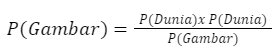
\includegraphics{Asset/image3.png}

Dalam persamaan ini, P(Dunia\textbar Gambar) merupakan Visi Komputer,
P(Dunia) mengacu pada pemodelan objek dalam dunia nyata, dan
P(Gambar\textbar Dunia) adalah Grafika Komputer. Perspektif ini
mendorong pendekatan pembelajaran statistik. Oleh karena itu, visi
komputer berkaitan dengan pengembangan mesin-mesin yang dapat melihat
dan berinteraksi dengan dunia.

Konsep ini diilustrasikan dalam Gambar 1.2.\\

\begin{figure}

{\centering 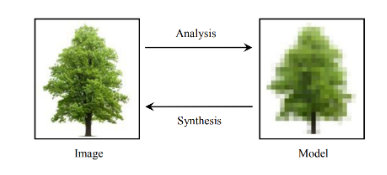
\includegraphics{Asset/image4.png}

}

\caption{Gambar 1.2: Visi Komputer vs Grafika Komputer}

\end{figure}

Visi komputer saat ini digunakan dalam berbagai aplikasi dunia nyata,
termasuk inspeksi mesin, pengenalan karakter optik (OCR), pembangunan
model 3D (fotogrametri), analisis gambar medis, pengawasan video
otomatis, biometrik, fusi dan penyambungan gambar, morphing, pemodelan
3D, dan lain-lain. Seperti yang ditunjukkan dalam Gambar 1.3., visi
komputer terkait dengan banyak bidang penelitian penting.

\begin{figure}

{\centering 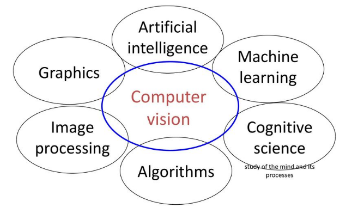
\includegraphics{Asset/image5.png}

}

\caption{Gambar 1.3: Computer vision dan disiplin terkait}

\end{figure}

Selain itu, visi komputer juga menghadapi tantangan etika dan privasi.
Penggunaan visi komputer dalam pengawasan dan pengenalan wajah telah
menimbulkan pertanyaan tentang privasi dan hak individu. Bagaimana data
visual dikumpulkan, digunakan, dan disimpan perlu diatur dengan
hati-hati untuk melindungi privasi individu dan mencegah penyalahgunaan
teknologi.

Namun, dengan penelitian dan pengembangan yang berkelanjutan, visi
komputer, sebagai subbidang ilmu komputer dengan tujuan membangun mesin
agar bisa memproses dan menginterpretasikan gambar dan video seperti
yang dilakukan sistem visual manusia, terus berkembang dan memperbaiki
keterbatasannya, menawarkan prospek yang menjanjikan untuk masa depan.

\hypertarget{b.-pengenalan-python}{%
\section*{B. Pengenalan Python}\label{b.-pengenalan-python}}
\addcontentsline{toc}{section}{B. Pengenalan Python}

\markright{B. Pengenalan Python}

Python adalah sebuah bahasa pemrograman yang telah matang dan menawarkan
sifat open source, yang berarti kode sumbernya tersedia secara bebas dan
dapat diubah atau dikembangkan lebih lanjut oleh siapa saja. Sebagai
bahasa yang mudah dipelajari, Python telah berhasil mengumpulkan basis
pengguna yang sangat luas. Komunitas ini, yang terdiri dari jutaan
pengguna di seluruh dunia, siap membantu Anda mengembangkan keterampilan
dan pemahaman Anda tentang Python, baik Anda seorang pemula atau
programmer berpengalaman.

Basis pengguna Python, yang beragam dan aktif, telah berkontribusi pada
pengembangan berbagai alat dan perpustakaan pendukung. Perpustakaan ini
adalah kumpulan rutinitas yang telah dikompilasi sebelumnya, dan
dirancang untuk memfasilitasi berbagai upaya ilmiah dan teknis. Mulai
dari data science, machine learning, pemrosesan bahasa, robotika, hingga
visi komputer, Python telah memberikan solusi yang kuat dan fleksibel.
Itulah sebabnya Python telah menjadi salah satu bahasa komputasi ilmiah
yang paling penting, baik dalam lingkungan akademisi maupun industri.

Popularitas Python tentu saja datang dengan tantangannya sendiri.
Seperti hutan belantara, ekosistem Python telah berkembang menjadi
sesuatu yang tampak rumit dan sulit ditembus. Beberapa ilmuwan dan
profesional baru dalam dunia Python mungkin merasa frustrasi dan stres
saat berhadapan dengan banyaknya pilihan yang tersedia. Mereka harus
membuat keputusan penting seperti perpustakaan mana yang harus digunakan
untuk menggambar grafik atau editor teks mana yang harus digunakan untuk
menulis program mereka.

Fleksibilitas Python datang sebagai solusi. Python mampu menangani
berbagai format data, menjalankan peralatan ilmiah, dan berintegrasi
dengan bahasa tingkat rendah seperti C, C++, dan FORTRAN. Python dapat
digunakan sebagai ``bahasa perekat'', memungkinkan integrasi berbagai
skrip atau sistem yang berbeda. Jadi, meskipun ada banyak pilihan,
Python menawarkan kemampuan untuk memilih dan menyesuaikan sesuai dengan
kebutuhan spesifik Anda, yang menjadikannya lebih mudah bagi pengguna
baru untuk memulai dan berkembang.

\hypertarget{c.-python-untuk-computer-vision}{%
\section*{C. Python untuk Computer
Vision}\label{c.-python-untuk-computer-vision}}
\addcontentsline{toc}{section}{C. Python untuk Computer Vision}

\markright{C. Python untuk Computer Vision}

Computer Vision adalah sebuah cabang dari ilmu komputer yang
memungkinkan mesin untuk memahami dan memanipulasi konten visual. Dengan
adanya teknologi ini, kita bisa mendapatkan banyak keuntungan seperti
dalam pengenalan wajah, deteksi objek, hingga analisis gambar dan video
dalam bidang medis. Dalam bidang ini, Python telah menjadi bahasa
pemrograman yang sangat berharga dan penting.

Python adalah bahasa pemrograman yang telah matang dan terbuka
(open-source), membuatnya menjadi pilihan yang sangat baik untuk
computer vision. Python menyediakan sintaks yang mudah dibaca dan
dipahami, sehingga memudahkan pengguna baru untuk memahami dan
memanfaatkan berbagai perpustakaan pendukung yang tersedia untuk
computer vision. Di antara perpustakaan tersebut, ada OpenCV,
TensorFlow, dan PyTorch, yang semuanya penting untuk pengembangan dan
implementasi solusi computer vision.

OpenCV (Open Source Computer Vision Library) adalah perpustakaan yang
sangat populer dalam bidang pengolahan gambar dan computer vision.
Dikembangkan oleh Intel dan disebarkan dengan lisensi BSD, OpenCV
memungkinkan pengembangan solusi computer vision dengan cepat dan
efisien, baik untuk aplikasi real-time maupun offline.

Sementara itu, TensorFlow dan PyTorch adalah kerangka kerja pembelajaran
mesin yang mendukung operasi yang diperlukan untuk pekerjaan computer
vision. Keduanya mendukung teknik pembelajaran mesin canggih seperti
jaringan saraf dan pembelajaran mendalam (deep learning) yang sering
digunakan dalam aplikasi computer vision modern.

Python juga memiliki kelebihan dalam penanganan data visual. Dengan
Python, pengguna dapat dengan mudah membaca, menulis, dan memanipulasi
gambar dan video dalam berbagai format. Python juga mendukung operasi
pra-pemrosesan yang diperlukan untuk data visual, seperti perubahan
ukuran gambar, normalisasi, dan augmentasi data.

Terakhir, Python juga menawarkan kemudahan dalam visualisasi data dan
hasil. Dengan menggunakan perpustakaan seperti Matplotlib dan Seaborn,
pengguna dapat dengan mudah memvisualisasikan data dan hasil dalam
berbagai format.\\
Dengan kata lain, dengan Python, computer vision menjadi lebih mudah
diakses dan dipahami, baik oleh profesional maupun pemula. Python telah
membuktikan dirinya sebagai bahasa pemrograman yang kuat dan fleksibel
yang dapat mendukung berbagai tugas dan proyek dalam bidang computer
vision.

\hypertarget{d.-latihan-praktik}{%
\section*{D. Latihan Praktik}\label{d.-latihan-praktik}}
\addcontentsline{toc}{section}{D. Latihan Praktik}

\markright{D. Latihan Praktik}

Python merupakan bahasa pemrograman yang ideal untuk belajar dan
menerapkan visi komputer. Berikut adalah beberapa latihan praktik yang
dapat Anda lakukan untuk meningkatkan keterampilan visi komputer Anda
menggunakan Python.

\textbf{Latihan 1:} Membaca dan Menampilkan Gambar

Tujuan dari latihan ini adalah untuk memahami cara membaca dan
menampilkan gambar menggunakan Python dan OpenCV, sebuah pustaka yang
sering digunakan dalam visi komputer.

\begin{Shaded}
\begin{Highlighting}[]
\ImportTok{import}\NormalTok{ cv2}

\CommentTok{\# Membaca gambar}
\NormalTok{gambar }\OperatorTok{=}\NormalTok{ cv2.imread(}\StringTok{\textquotesingle{}namafile.jpg\textquotesingle{}}\NormalTok{)}

\CommentTok{\# Menampilkan gambar}
\NormalTok{cv2.imshow(}\StringTok{\textquotesingle{}Gambar\textquotesingle{}}\NormalTok{, gambar)}
\NormalTok{cv2.waitKey(}\DecValTok{0}\NormalTok{)}
\NormalTok{cv2.destroyAllWindows()}
\end{Highlighting}
\end{Shaded}

\begin{tcolorbox}[enhanced jigsaw, opacityback=0, colbacktitle=quarto-callout-tip-color!10!white, breakable, titlerule=0mm, left=2mm, toptitle=1mm, rightrule=.15mm, leftrule=.75mm, colback=white, opacitybacktitle=0.6, arc=.35mm, toprule=.15mm, coltitle=black, colframe=quarto-callout-tip-color-frame, bottomtitle=1mm, title=\textcolor{quarto-callout-tip-color}{\faLightbulb}\hspace{0.5em}{Penjelasan Kode}, bottomrule=.15mm]

\begin{itemize}
\item
  import cv2: Ini adalah perintah untuk mengimpor library OpenCV (cv2)
  ke dalam program Python. OpenCV adalah library populer yang digunakan
  untuk memanipulasi gambar dan video.
\item
  gambar = cv2.imread(`namafile.jpg'): Baris ini membaca gambar dengan
  nama file `namafile.jpg' menggunakan fungsi imread() dari OpenCV.
  Fungsi ini mengembalikan matriks NumPy yang mewakili gambar.
\item
  cv2.imshow(`Gambar', gambar): Ini adalah perintah untuk menampilkan
  gambar ke jendela dengan judul `Gambar'. Fungsi imshow() dari OpenCV
  digunakan untuk menampilkan gambar dalam jendela.
\item
  cv2.waitKey(0): Baris ini menunggu pengguna menekan tombol apa pun
  untuk melanjutkan eksekusi program. Nilai argumen 0 menunjukkan bahwa
  program akan tetap berjalan sampai tombol ditekan.
\item
  cv2.destroyAllWindows(): Ini adalah perintah untuk menutup semua
  jendela yang dibuka oleh program. Fungsi destroyAllWindows() digunakan
  untuk membersihkan semua jendela tampilan.\\
\end{itemize}

\end{tcolorbox}

\textbf{Latihan 2:} Mengubah Gambar ke Grayscale

Banyak operasi dalam visi komputer dijalankan pada gambar grayscale.
Latihan ini bertujuan untuk mengubah gambar berwarna menjadi grayscale.

\begin{Shaded}
\begin{Highlighting}[]
\ImportTok{import}\NormalTok{ cv2}

\CommentTok{\# Membaca gambar}
\NormalTok{gambar }\OperatorTok{=}\NormalTok{ cv2.imread(}\StringTok{\textquotesingle{}namafile.jpg\textquotesingle{}}\NormalTok{)}

\CommentTok{\# Mengubah gambar ke grayscale}
\NormalTok{gray }\OperatorTok{=}\NormalTok{ cv2.cvtColor(gambar, cv2.COLOR\_BGR2GRAY)}

\CommentTok{\# Menampilkan gambar grayscale}
\NormalTok{cv2.imshow(}\StringTok{\textquotesingle{}Gambar Grayscale\textquotesingle{}}\NormalTok{, gray)}
\NormalTok{cv2.waitKey(}\DecValTok{0}\NormalTok{)}
\NormalTok{cv2.destroyAllWindows()}
\end{Highlighting}
\end{Shaded}

\begin{tcolorbox}[enhanced jigsaw, opacityback=0, colbacktitle=quarto-callout-tip-color!10!white, breakable, titlerule=0mm, left=2mm, toptitle=1mm, rightrule=.15mm, leftrule=.75mm, colback=white, opacitybacktitle=0.6, arc=.35mm, toprule=.15mm, coltitle=black, colframe=quarto-callout-tip-color-frame, bottomtitle=1mm, title=\textcolor{quarto-callout-tip-color}{\faLightbulb}\hspace{0.5em}{Penjelasan Kode}, bottomrule=.15mm]

\begin{itemize}
\tightlist
\item
  gray = cv2.cvtColor(gambar, cv2.COLOR\_BGR2GRAY): Baris ini mengubah
  gambar dari warna (BGR) ke skala keabuan (grayscale) menggunakan
  fungsi cvtColor() dari OpenCV. Fungsi ini menerima dua argumen, yaitu
  gambar yang ingin diubah (variabel gambar) dan konversi warna yang
  ingin dilakukan (dalam hal ini, dari BGR ke grayscale). Hasil konversi
  disimpan dalam variabel gray.\\
\end{itemize}

\end{tcolorbox}

\textbf{Latihan 3:} Deteksi Tepi

Deteksi tepi adalah teknik penting dalam visi komputer. Latihan ini
bertujuan untuk menerapkan deteksi tepi pada gambar.

\begin{Shaded}
\begin{Highlighting}[]
\ImportTok{import}\NormalTok{ cv2}
\ImportTok{import}\NormalTok{ numpy }\ImportTok{as}\NormalTok{ np}

\CommentTok{\# Membaca gambar}
\NormalTok{gambar }\OperatorTok{=}\NormalTok{ cv2.imread(}\StringTok{\textquotesingle{}namafile.jpg\textquotesingle{}}\NormalTok{)}

\CommentTok{\# Mengubah gambar ke grayscale}
\NormalTok{gray }\OperatorTok{=}\NormalTok{ cv2.cvtColor(gambar, cv2.COLOR\_BGR2GRAY)}

\CommentTok{\# Mengaplikasikan deteksi tepi}
\NormalTok{edges }\OperatorTok{=}\NormalTok{ cv2.Canny(gray, }\DecValTok{30}\NormalTok{, }\DecValTok{100}\NormalTok{)}

\CommentTok{\# Menampilkan gambar dengan tepi yang terdeteksi}
\NormalTok{cv2.imshow(}\StringTok{\textquotesingle{}Deteksi Tepi\textquotesingle{}}\NormalTok{, edges)}
\NormalTok{cv2.waitKey(}\DecValTok{0}\NormalTok{)}
\NormalTok{cv2.destroyAllWindows()}
\end{Highlighting}
\end{Shaded}

\begin{tcolorbox}[enhanced jigsaw, opacityback=0, colbacktitle=quarto-callout-tip-color!10!white, breakable, titlerule=0mm, left=2mm, toptitle=1mm, rightrule=.15mm, leftrule=.75mm, colback=white, opacitybacktitle=0.6, arc=.35mm, toprule=.15mm, coltitle=black, colframe=quarto-callout-tip-color-frame, bottomtitle=1mm, title=\textcolor{quarto-callout-tip-color}{\faLightbulb}\hspace{0.5em}{Penjelasan Kode}, bottomrule=.15mm]

\begin{itemize}
\tightlist
\item
  edges = cv2.Canny(gray, 30, 100): Baris ini menerapkan deteksi tepi
  pada gambar skala keabuan (grayscale) menggunakan metode Canny dengan
  parameter threshold lower dan upper sebesar 30 dan 100. Fungsi Canny()
  dari OpenCV menghasilkan gambar dengan tepi yang terdeteksi, yang
  disimpan dalam variabel edges.\\
\end{itemize}

\end{tcolorbox}

\textbf{Latihan 4:} Deteksi Wajah

Pustaka OpenCV menyediakan pretrained cascade classifiers yang dapat
digunakan untuk deteksi wajah dan fitur wajah lainnya.

\begin{Shaded}
\begin{Highlighting}[]
\ImportTok{import}\NormalTok{ cv2}

\CommentTok{\# Membaca gambar}
\NormalTok{gambar }\OperatorTok{=}\NormalTok{ cv2.imread(}\StringTok{\textquotesingle{}namafile.jpg\textquotesingle{}}\NormalTok{)}

\CommentTok{\# Mengubah gambar ke grayscale}
\NormalTok{gray }\OperatorTok{=}\NormalTok{ cv2.cvtColor(gambar, cv2.COLOR\_BGR2GRAY)}

\CommentTok{\# Membuat objek face cascade}
\NormalTok{face\_cascade }\OperatorTok{=}\NormalTok{ cv2.CascadeClassifier(cv2.data.haarcascades }\OperatorTok{+} \StringTok{"haarcascade\_frontalface\_default.xml"}\NormalTok{)}

\CommentTok{\# Mendeteksi wajah}
\NormalTok{faces }\OperatorTok{=}\NormalTok{ face\_cascade.detectMultiScale(gray, scaleFactor}\OperatorTok{=}\FloatTok{1.1}\NormalTok{, minNeighbors}\OperatorTok{=}\DecValTok{5}\NormalTok{, minSize}\OperatorTok{=}\NormalTok{(}\DecValTok{30}\NormalTok{, }\DecValTok{30}\NormalTok{))}

\CommentTok{\# Menggambar kotak pada setiap wajah yang terdeteksi}
\ControlFlowTok{for}\NormalTok{ (x, y, w, h) }\KeywordTok{in}\NormalTok{ faces:}
\NormalTok{    cv2.rectangle(gambar, (x, y), (x}\OperatorTok{+}\NormalTok{w, y}\OperatorTok{+}\NormalTok{h), (}\DecValTok{0}\NormalTok{, }\DecValTok{255}\NormalTok{, }\DecValTok{0}\NormalTok{), }\DecValTok{2}\NormalTok{)}

\CommentTok{\# Menampilkan gambar dengan wajah yang terdeteksi}
\NormalTok{cv2.imshow(}\StringTok{\textquotesingle{}Deteksi Wajah\textquotesingle{}}\NormalTok{, gambar)}
\NormalTok{cv2.waitKey(}\DecValTok{0}\NormalTok{)}
\NormalTok{cv2.destroyAllWindows()}
\end{Highlighting}
\end{Shaded}

\begin{tcolorbox}[enhanced jigsaw, opacityback=0, colbacktitle=quarto-callout-tip-color!10!white, breakable, titlerule=0mm, left=2mm, toptitle=1mm, rightrule=.15mm, leftrule=.75mm, colback=white, opacitybacktitle=0.6, arc=.35mm, toprule=.15mm, coltitle=black, colframe=quarto-callout-tip-color-frame, bottomtitle=1mm, title=\textcolor{quarto-callout-tip-color}{\faLightbulb}\hspace{0.5em}{Penjelasan Kode}, bottomrule=.15mm]

\begin{itemize}
\item
  face\_cascade = cv2.CascadeClassifier(cv2.data.haarcascades +
  ``haarcascade\_frontalface\_default.xml''): Baris ini membuat objek
  cascade classifier untuk mendeteksi wajah. Cascade classifier adalah
  algoritma yang digunakan untuk mendeteksi objek dalam gambar
  berdasarkan fitur-fitur yang telah ditraining sebelumnya. Dalam hal
  ini, digunakan cascade classifier untuk mendeteksi wajah dengan
  menggunakan file XML yang disebut
  ``haarcascade\_frontalface\_default.xml''. File XML ini berisi
  informasi tentang fitur-fitur yang relevan untuk mendeteksi wajah.
\item
  faces = face\_cascade.detectMultiScale(gray, scaleFactor=1.1,
  minNeighbors=5, minSize=(30, 30)): Baris ini mendeteksi wajah dalam
  gambar menggunakan metode detectMultiScale() dari cascade classifier.
  Metode ini menerima gambar skala keabuan (gray) sebagai input dan
  mengembalikan array yang berisi koordinat wajah yang terdeteksi.
  Parameter-parameter yang digunakan adalah scaleFactor (faktor skala
  untuk deteksi multi-skala), minNeighbors (jumlah minimum tetangga yang
  harus ada agar wajah dianggap valid), dan minSize (ukuran minimum
  wajah yang diterima).
\item
  for (x, y, w, h) in faces: cv2.rectangle(gambar, (x, y), (x+w, y+h),
  (0, 255, 0), 2): Baris ini menggunakan loop untuk menggambar kotak
  pada setiap wajah yang terdeteksi. Koordinat dan ukuran wajah yang
  terdeteksi (x, y, w, h) diperoleh dari array wajah yang ditemukan
  sebelumnya. Kotak tersebut digambar menggunakan fungsi rectangle()
  dari OpenCV pada gambar asli (variabel gambar).\\
\end{itemize}

\end{tcolorbox}

Harap diingat bahwa setiap latihan ini hanyalah awal. Visi komputer
adalah bidang yang sangat luas dengan banyak teknik dan algoritma yang
berbeda. Untuk benar-benar mahir, Anda perlu memahami teori di balik
teknik ini dan bagaimana menerapkannya dalam situasi nyata.

\hypertarget{e.-sesi-tanya-jawab-dan-diskusi}{%
\section*{E. Sesi Tanya Jawab dan
Diskusi}\label{e.-sesi-tanya-jawab-dan-diskusi}}
\addcontentsline{toc}{section}{E. Sesi Tanya Jawab dan Diskusi}

\markright{E. Sesi Tanya Jawab dan Diskusi}

Q: Apa itu computer vision dan mengapa itu penting?

A: Computer vision adalah bidang teknologi yang memungkinkan komputer
dan mesin untuk `melihat' dan memahami konten visual, seperti gambar dan
video. Computer vision penting karena memungkinkan automasi dan analisis
tingkat lanjut dalam berbagai bidang, seperti keamanan, kesehatan,
manufaktur, dan banyak lagi.

Q: Mengapa Python sering digunakan dalam computer vision?

A: Python sering digunakan dalam computer vision karena mudah
dipelajari, memiliki sintaks yang jelas dan bersih, dan didukung oleh
banyak library dan framework yang kuat seperti OpenCV, TensorFlow, dan
PyTorch. Python juga open-source, yang berarti kode sumbernya tersedia
secara bebas dan dapat dimodifikasi atau diperluas oleh komunitas.

Q: Bagaimana saya bisa belajar lebih banyak tentang computer vision dan
Python?

A: Anda bisa memulai dengan belajar dasar-dasar Python dan lalu belajar
tentang perpustakaan seperti OpenCV, TensorFlow, dan PyTorch. Anda juga
bisa mengikuti and 1 attachments

Q: Saya baru belajar Python, apakah saya bisa belajar Computer Vision?

A: Ya, Anda bisa belajar Computer Vision meski baru belajar Python.
Sebenarnya, Python adalah bahasa pemrograman yang baik untuk dipelajari
jika Anda tertarik dengan Computer Vision karena memiliki banyak library
dan framework, seperti OpenCV, TensorFlow, dan PyTorch, yang dirancang
khusus untuk visi komputer dan pembelajaran mesin.

Q: Apa yang dimaksud dengan Object Detection dalam Computer Vision?

A: Object Detection adalah teknologi dalam visi komputer yang
mengidentifikasi atau mendeteksi objek dari berbagai kelas (seperti
manusia, kendaraan, atau hewan) dalam gambar atau video. Teknologi ini
biasanya digunakan dalam aplikasi seperti pengawasan video, sistem
navigasi untuk kendaraan otonom, dan banyak lagi.

Q: Apakah memungkinkan untuk melakukan Computer Vision tanpa Machine
Learning?

A: Ya, memang memungkinkan untuk melakukan tugas-tugas visi komputer
tertentu tanpa menggunakan Machine Learning. Misalnya, teknik seperti
pengolahan gambar, deteksi tepi, dan thresholding bisa digunakan untuk
ekstraksi fitur dan pemrosesan gambar dasar. Namun, untuk tugas yang
lebih kompleks seperti deteksi objek, pengenalan wajah, dan analisis
video, biasanya diperlukan teknik Machine Learning atau Deep Learning.

\hypertarget{python}{%
\chapter*{2 Python}\label{python}}
\addcontentsline{toc}{chapter}{2 Python}

\markboth{2 Python}{2 Python}

\hypertarget{a.-dasar-dasar-python}{%
\section*{A. Dasar-dasar Python}\label{a.-dasar-dasar-python}}
\addcontentsline{toc}{section}{A. Dasar-dasar Python}

\markright{A. Dasar-dasar Python}

\hypertarget{apa-itu-python}{%
\subsection*{Apa itu Python?}\label{apa-itu-python}}
\addcontentsline{toc}{subsection}{Apa itu Python?}

Python adalah bahasa pemrograman tingkat tinggi yang populer. Bahasa ini
dapat menangani berbagai tugas pemrograman seperti komputasi numerik,
pengembangan web, pemrograman basis data, pemrograman jaringan,
pemrosesan paralel, dan lainnya.\\
Python populer karena berbagai alasan, termasuk:

\begin{itemize}
\tightlist
\item
  Bahasa ini gratis.\\
\item
  Tersedia di semua sistem operasi populer seperti Windows, Mac, atau
  Linux.\\
\item
  Python adalah bahasa yang diinterpretasikan. Oleh karena itu,
  pemrogram dapat menguji bagian kode di baris perintah sebelum
  menggabungkannya ke dalam program mereka. Tidak ada kebutuhan untuk
  kompilasi atau penghubungan. Python memungkinkan pemrograman yang
  lebih cepat.\\
\item
  Python lebih sederhana secara sintaksis dibandingkan dengan
  C/C++/Fortran. Oleh karena itu, Python sangat mudah dibaca dan lebih
  mudah untuk debug.\\
\item
  Python datang dengan berbagai modul yang standar atau dapat diinstal
  dalam instalasi Python yang ada. Modul-modul ini dapat melakukan
  berbagai tugas seperti membaca dan menulis berbagai file, komputasi
  ilmiah, visualisasi data, dan lainnya.\\
\item
  Program yang ditulis dalam Python dapat dijalankan di berbagai sistem
  operasi atau platform dengan sedikit atau tanpa perubahan.\\
\item
  Python adalah bahasa yang dinamis dalam pengetikannya. Oleh karena
  itu, tipe data dari variabel tidak harus dinyatakan sebelum
  penggunaannya, membuatnya lebih mudah untuk orang dengan pengalaman
  coding yang kurang.\\
\item
  Python memiliki komunitas pengembang dan pengguna yang berdedikasi dan
  selalu diperbarui.\\
  Meskipun Python memiliki banyak keunggulan yang membuatnya menjadi
  salah satu bahasa yang diinterpretasikan paling populer, Python
  memiliki beberapa kelemahan yang dibahas di bawah ini:\\
\item
  Karena fokus Python adalah pada kemampuan untuk pemrograman yang lebih
  cepat, kecepatan eksekusi menderita. Program Python mungkin 10 kali
  atau lebih lambat (misalnya) dibandingkan dengan program C yang
  setara, tetapi program Python akan berisi lebih sedikit baris kode dan
  dapat diprogram untuk menangani berbagai jenis data dengan mudah.
  Kelemahan ini dalam kode Python dapat diatasi dengan mengubah bagian
  kode yang intensif secara komputasi ke C/C++ atau dengan penggunaan
  struktur data dan modul yang tepat.\\
\item
  Indentasi kode tidak opsional. Ini membuat kode mudah dibaca. Namun,
  kode dengan loop dan konstruk lainnya akan diindentasi ke kanan,
  membuatnya sulit untuk membaca kode.
\end{itemize}

\hypertarget{lingkungan-python}{%
\subsection*{Lingkungan Python}\label{lingkungan-python}}
\addcontentsline{toc}{subsection}{Lingkungan Python}

Terdapat beberapa lingkungan Python yang dapat dipilih. Beberapa sistem
operasi seperti Mac, Linux, Unix, dan lainnya memiliki interpreter
bawaan. Interpreter tersebut mungkin mengandung semua modul tetapi tidak
siap pakai untuk komputasi ilmiah. Distribusi khusus telah dibuat dan
dijual kepada komunitas ilmiah, dibangun sebelumnya dengan berbagai
modul ilmiah Python. Saat menggunakan distribusi ini, pengguna tidak
perlu menginstal modul ilmiah secara individual. Jika modul tertentu
yang diminati tidak tersedia dalam distribusi, modul tersebut dapat
diinstal. Salah satu distribusi paling populer adalah Anaconda.
Instruksi untuk menginstal distribusi Anaconda dapat ditemukan di
\href{https://www.anaconda.com/distribution/}{www.anaconda.com}

\hypertarget{interpreter-python}{%
\subsubsection*{Interpreter Python}\label{interpreter-python}}
\addcontentsline{toc}{subsubsection}{Interpreter Python}

Interpreter Python yang terintegrasi dalam sebagian besar sistem operasi
dapat dimulai dengan hanya mengetik python di jendela terminal. Ketika
interpreter dimulai, prompt perintah
(\textgreater\textgreater\textgreater) muncul. Perintah Python dapat
dimasukkan di prompt untuk diproses. Misalnya, di Windows, ketika
interpreter Python bawaan dimulai, output yang mirip dengan yang
ditunjukkan di bawah ini muncul:

\begin{figure}

{\centering 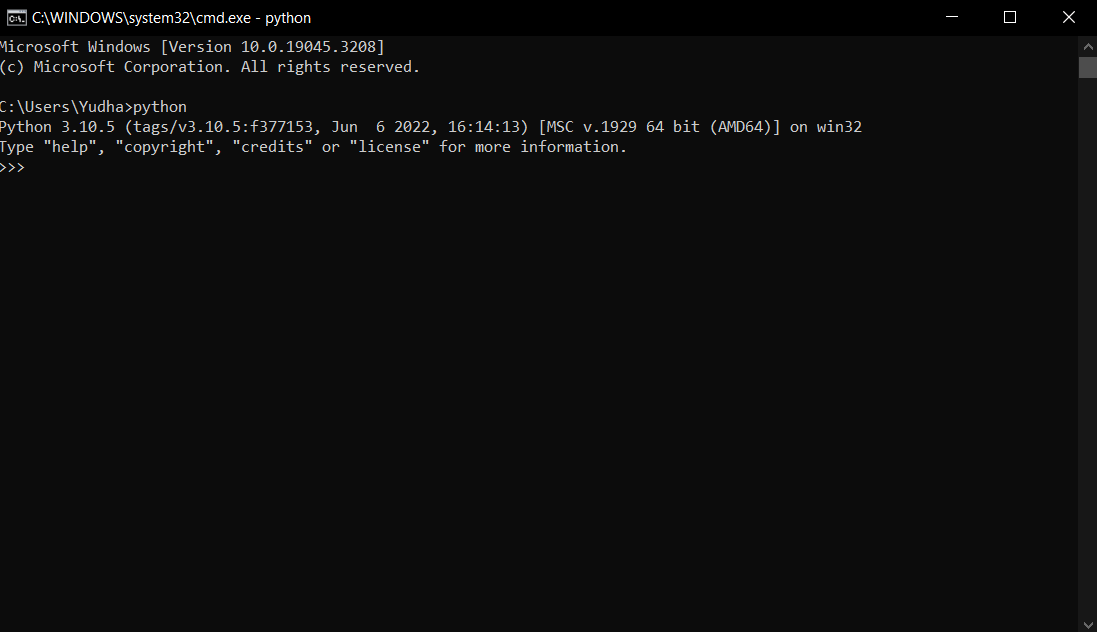
\includegraphics{Asset/image6.png}

}

\caption{Gambar 2.1. Terminal Python}

\end{figure}

\begin{tcolorbox}[enhanced jigsaw, opacityback=0, colbacktitle=quarto-callout-tip-color!10!white, breakable, titlerule=0mm, left=2mm, toptitle=1mm, rightrule=.15mm, leftrule=.75mm, colback=white, opacitybacktitle=0.6, arc=.35mm, toprule=.15mm, coltitle=black, colframe=quarto-callout-tip-color-frame, bottomtitle=1mm, title=\textcolor{quarto-callout-tip-color}{\faLightbulb}\hspace{0.5em}{Tip}, bottomrule=.15mm]

Perhatikan bahwa dalam contoh di atas, interpreter Python adalah versi
3.10.5. Kemungkinan Anda mungkin memiliki versi yang berbeda.

\end{tcolorbox}

\hypertarget{distribusi-python}{%
\subsubsection*{Distribusi Python}\label{distribusi-python}}
\addcontentsline{toc}{subsubsection}{Distribusi Python}

Distribusi Python Anaconda menyediakan hampir 100 modul Python ilmiah
paling populer seperti perhitungan ilmiah, aljabar linear, komputasi
simbolik, pemrosesan gambar, pemrosesan sinyal, visualisasi, integrasi
program C/C++ ke Python, dll. Ini didistribusikan dan dikelola oleh
Continuum Analytics. Ini tersedia secara gratis untuk akademisi dan
tersedia dengan harga untuk semua orang lainnya. Selain berbagai modul
yang dibangun ke dalam Anaconda, pemrogram dapat menginstal modul lain
menggunakan manajer paket conda {[}Ana20b{]}, tanpa mempengaruhi
distribusi utama. Untuk mengakses Python dari baris perintah, mulailah
`Anaconda Prompt' yang dapat dieksekusi.

\begin{figure}

{\centering 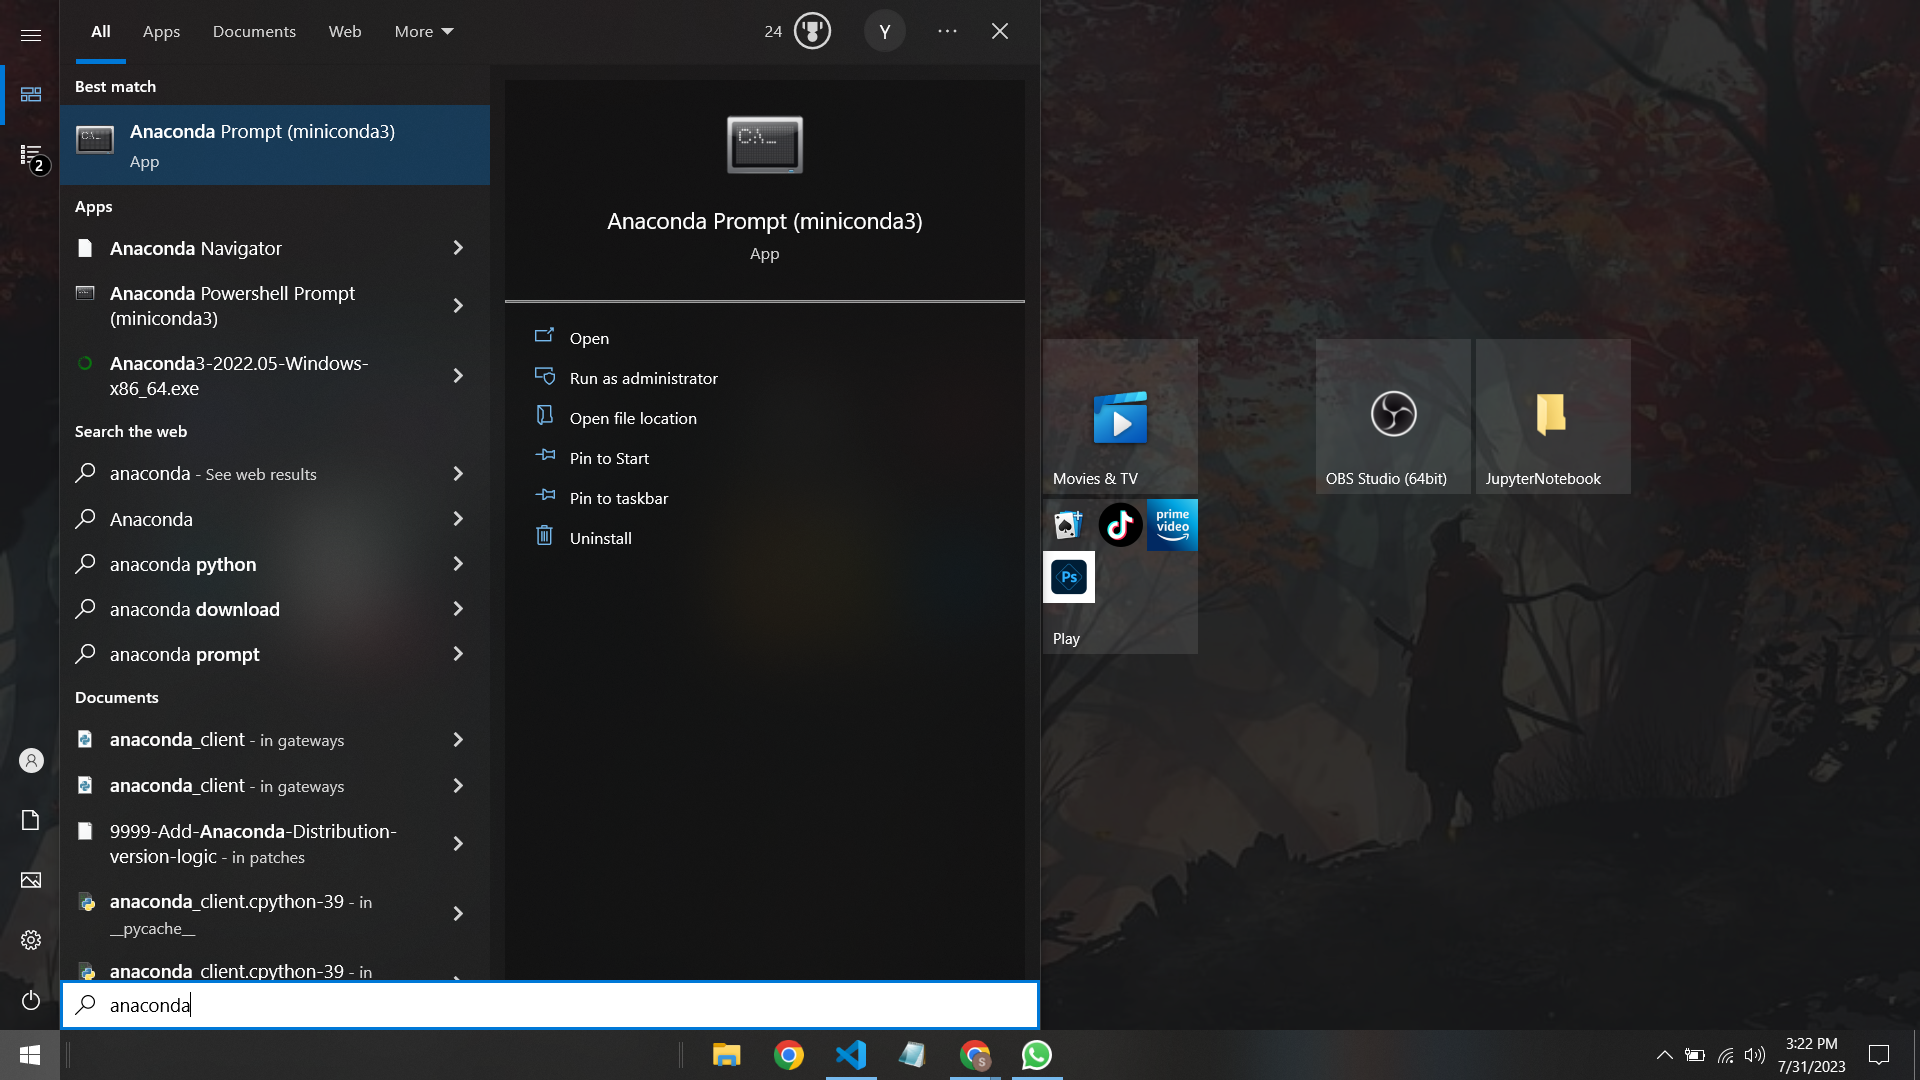
\includegraphics{Asset/image7.png}

}

\caption{Gambar 2.2. Mencari Anaconda Prompt}

\end{figure}

dan kemudian ketik python seperti pada Gambar 2.3.

\begin{figure}

{\centering 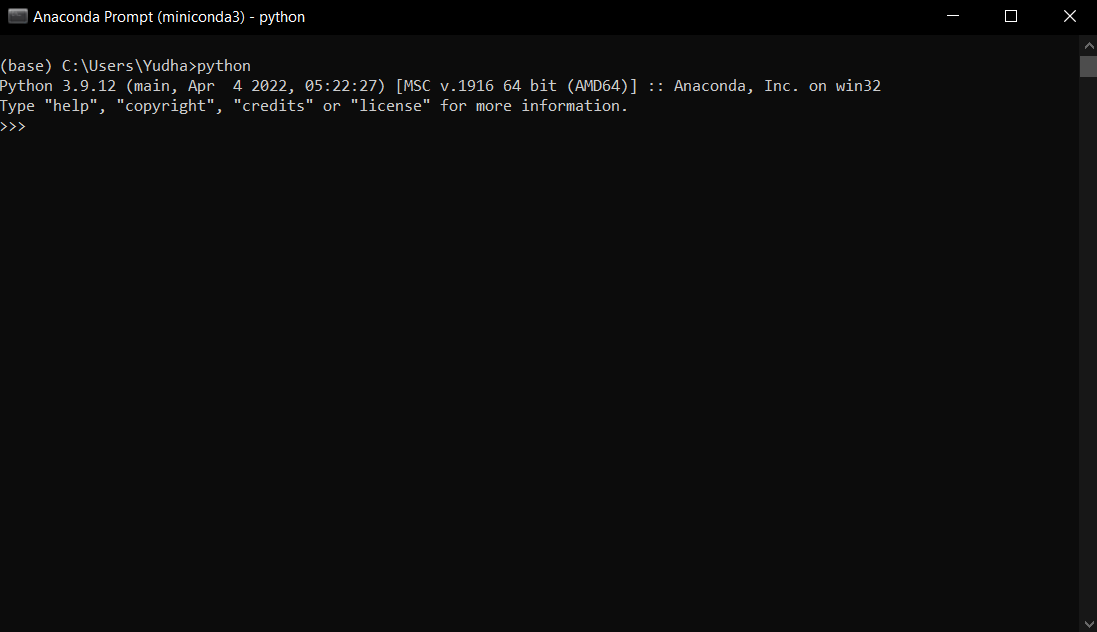
\includegraphics{Asset/image8.png}

}

\caption{Gambar 2.3. Terminal Anaconda}

\end{figure}

\hypertarget{instalasi-python-dan-lingkungannya}{%
\subsection*{Instalasi Python dan
Lingkungannya}\label{instalasi-python-dan-lingkungannya}}
\addcontentsline{toc}{subsection}{Instalasi Python dan Lingkungannya}

Instalasi Python:

\begin{itemize}
\tightlist
\item
  Unduh dan instal Python. Anda dapat mengunduh versi terbaru dari
  Python di situs web resmi Python, yaitu
  \href{https://www.python.org/}{www.python.org}. Pilih versi yang
  sesuai dengan sistem operasi dan arsitektur komputer Anda (32-bit atau
  64-bit).\\
\item
  Jalankan installer Python dan ikuti petunjuk yang ada. Pastikan untuk
  mencentang kotak yang mengatakan ``Add Python to PATH'' saat proses
  instalasi. Ini memudahkan Anda menjalankan Python dari command line.\\
\item
  Verifikasi instalasi Python dengan membuka terminal atau command
  prompt dan mengetik python --version. Anda seharusnya melihat versi
  Python yang baru saja Anda instal.
\end{itemize}

Instalasi Anaconda:

\begin{itemize}
\tightlist
\item
  Unduh dan instal Anaconda / Miniconda. Anda dapat mengunduh versi
  terbaru dari Anaconda di situs web resmi Anaconda, yaitu
  \href{https://www.anaconda.com/}{www.anaconda.com} . atau Miniconda
  \href{https://docs.conda.io/en/latest/miniconda.html}{link Miniconda}
  Pilih versi yang sesuai dengan sistem operasi dan arsitektur komputer
  Anda (32-bit atau 64-bit).
\item
  Jalankan installer dan ikuti petunjuk yang ada. Pastikan untuk
  mencentang kotak yang mengatakan ``Add Anaconda to my PATH variable''
  saat proses instalasi. Ini memudahkan Anda menjalankan Anaconda dari
  command line.
\item
  Verifikasi instalasi Anaconda dengan membuka terminal atau command
  prompt dan mengetik conda --version. Anda seharusnya melihat versi
  Anaconda / Miniconda yang baru saja Anda instal.
\end{itemize}

\url{https://youtu.be/k88q-4Bcr3Y}

Link repository yang terdapat pada
video.\href{https://github.com/yufaa/ComputerVision/blob/main/tensorflow-install-jul-2020.ipynb}{Klik
disini}

\hypertarget{menjalankan-program-python}{%
\subsection*{Menjalankan Program
Python}\label{menjalankan-program-python}}
\addcontentsline{toc}{subsection}{Menjalankan Program Python}

Menggunakan interpreter Python apa pun (bawaan atau dari distribusi),
Anda dapat menjalankan program Anda menggunakan perintah di sistem
operasi (OS) prompt perintah. Jika file firstprog.py adalah file Python
yang perlu dieksekusi, kemudian ketik perintah berikut ini di OS prompt
perintah.

\begin{Shaded}
\begin{Highlighting}[]
\NormalTok{python latihanPython.py}
\end{Highlighting}
\end{Shaded}

Simbol \textgreater\textgreater{} adalah prompt terminal dan
\textgreater\textgreater\textgreater{} mewakili prompt Python.
Pendekatan terbaik untuk menjalankan program Python di bawah sistem
operasi apa pun adalah dengan menggunakan Lingkungan Pengembangan
Terpadu seperti IDLE atau Spyder karena memberikan kemampuan untuk
mengedit file dan juga menjalankannya di bawah antarmuka yang sama.\\
Buka CMD lalu pindah Directiory menggunakan command cd.

\begin{figure}

{\centering 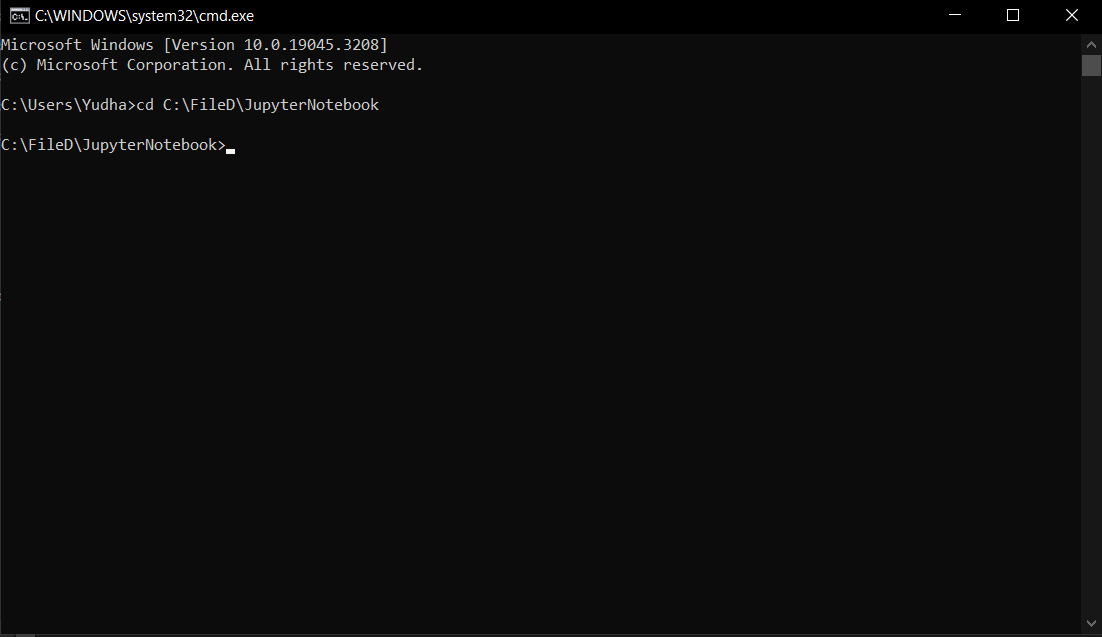
\includegraphics{Asset/image9.png}

}

\caption{Gambar 2.4. Terminal (Mengubah Directory)}

\end{figure}

Jalankan file dengan ekstensi .py seperti Gambar 2.5.

\begin{figure}

{\centering 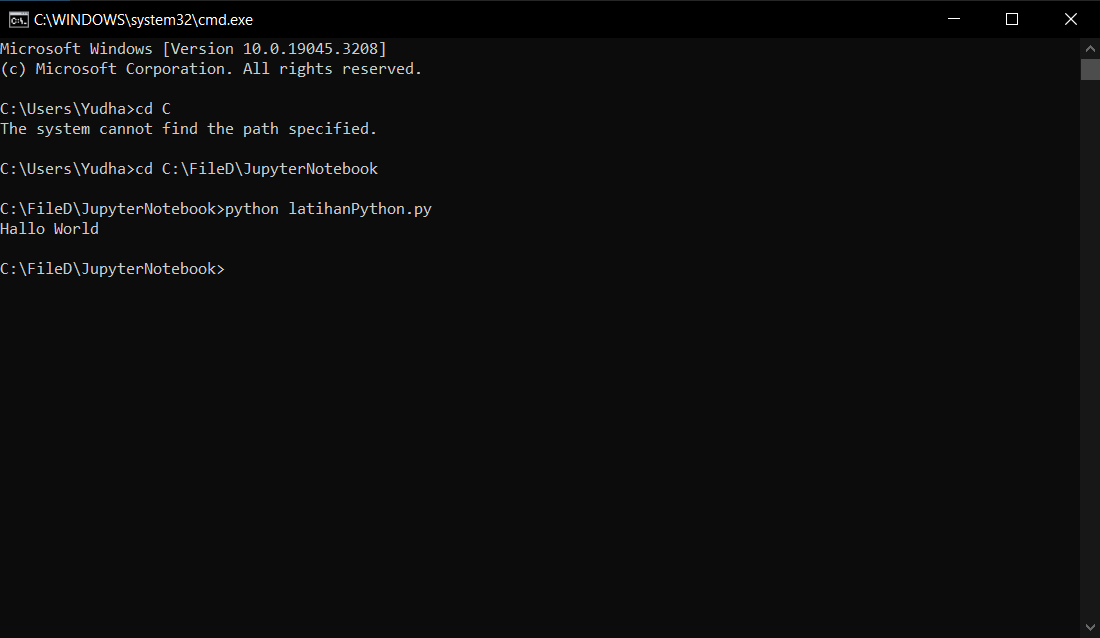
\includegraphics{Asset/image10.png}

}

\caption{Gambar 2.5. Terminal (Menjalankan Python)}

\end{figure}

\hypertarget{pernyataan-dasar-python-dan-jenis-data}{%
\subsection*{Pernyataan Dasar Python dan Jenis
Data}\label{pernyataan-dasar-python-dan-jenis-data}}
\addcontentsline{toc}{subsection}{Pernyataan Dasar Python dan Jenis
Data}

\textbf{Indentasi}\\
Dalam Python, blok kode ditunjukkan dengan indentasi. Misalnya dalam
kode di bawah ini, kita pertama-tama mencetak pesan, `Kami sedang
menghitung kuadrat dari angka antara 0 dan 9'. Kemudian kita melakukan
loop melalui nilai-nilai dalam rentang 0 hingga 9 dan menyimpannya dalam
variabel `i' dan juga mencetak kuadrat dari `i'. Akhirnya kita mencetak
pesan, 'Kami menyelesaikan tugas di akhir.\\
Dalam bahasa lain, blok kode di bawah for-loop akan diidentifikasi
dengan pasangan kurung kurawal \{\}. Namun, dalam Python kita tidak
menggunakan kurung kurawal. Blok kode diidentifikasi dengan menggeser
baris print(i*i) empat spasi ke kanan. Anda juga bisa memilih untuk
menggunakan tab sebagai gantinya.

\begin{Shaded}
\begin{Highlighting}[]
\BuiltInTok{print}\NormalTok{(}\StringTok{\textquotesingle{}Menghitung kuadrat dari angka antara 0 dan 9\textquotesingle{}}\NormalTok{) }
\ControlFlowTok{for}\NormalTok{ i }\KeywordTok{in} \BuiltInTok{range}\NormalTok{(}\DecValTok{10}\NormalTok{):}
    \BuiltInTok{print}\NormalTok{(i}\OperatorTok{*}\NormalTok{i)}
\BuiltInTok{print}\NormalTok{(}\StringTok{\textquotesingle{}Menyelesaikan tugas ...\textquotesingle{}}\NormalTok{)}
\end{Highlighting}
\end{Shaded}

Ada kelemahan signifikan dalam indentasi, terutama bagi pemrogram Python
baru. Sebuah kode yang berisi beberapa for-loop dan if-statements akan
diindentasi lebih jauh ke kanan membuat kode tidak dapat dibaca. Masalah
ini dapat diredakan dengan mengurangi jumlah for-loop dan if-statements.
Ini tidak hanya membuat kode dapat dibaca tetapi juga mengurangi waktu
komputasi. Ini dapat dicapai dengan pemrograman menggunakan struktur
data seperti daftar, kamus, dan set secara tepat.

\textbf{Komentar}\\
Komentar adalah bagian penting dari setiap bahasa pemrograman. Dalam
Python, komentar baris tunggal ditandai dengan hash \# di awal baris.
Beberapa baris dapat dikomentari dengan menggunakan string tanda kutip
tiga (tanda kutip tunggal tiga kali atau tanda kutip ganda tiga kali) di
awal dan di akhir blok.

\begin{Shaded}
\begin{Highlighting}[]
\CommentTok{\# Ini adalah komentar baris tunggal}
\CommentTok{"""}
\CommentTok{Ini adalah komentar multiline}
\CommentTok{"""}
\CommentTok{\# Komentar adalah cara yang baik untuk menjelaskan kode.}
\end{Highlighting}
\end{Shaded}

\textbf{Variabel}\\
Python adalah bahasa dinamis dan oleh karena itu Anda tidak perlu
menentukan jenis variabel seperti dalam C/C++. Variabel bisa dianggap
sebagai wadah nilai. Nilai tersebut bisa berupa bilangan bulat, float,
string, daftar, tuple, kamus, set, dll.

\begin{Shaded}
\begin{Highlighting}[]
\NormalTok{a }\OperatorTok{=} \DecValTok{1}
\NormalTok{a }\OperatorTok{=} \FloatTok{10.0}
\NormalTok{a }\OperatorTok{=} \StringTok{\textquotesingle{}hello\textquotesingle{}}
\end{Highlighting}
\end{Shaded}

Dalam contoh di atas nilai bilangan bulat 1, nilai float 10.0, dan nilai
string hello untuk semua kasus disimpan dalam variabel yang sama. Namun,
hanya nilai yang terakhir ditugaskan yang merupakan nilai saat ini untuk
a.

\textbf{Operator}\\
Python mendukung semua operator aritmatika umum seperti +, ---, *, /.
Juga mendukung operator perbandingan umum seperti \textgreater,
\textless, ==, ! =, \textgreater=, \textless=, dll. Selain itu, melalui
berbagai modul Python menyediakan banyak operator untuk melakukan
operasi trigonometri, matematika, geometri, dll.

\textbf{Loop}\\
Konstruksi looping yang paling umum dalam Python adalah pernyataan
for-loop, yang memungkinkan iterasi melalui kumpulan objek. Berikut ini
adalah contohnya:

\begin{Shaded}
\begin{Highlighting}[]
\ControlFlowTok{for}\NormalTok{ i }\KeywordTok{in} \BuiltInTok{range}\NormalTok{(}\DecValTok{1}\NormalTok{,}\DecValTok{5}\NormalTok{): }
    \BuiltInTok{print}\NormalTok{(i)}
\end{Highlighting}
\end{Shaded}

Dalam contoh di atas output dari for-loop adalah angka dari 1 hingga 5.
Fungsi range memungkinkan kita untuk membuat nilai mulai dari 1 dan
berakhir dengan 5. Konsep semacam ini mirip dengan for-loop yang
biasanya ditemukan dalam C/C++ atau sebagian besar bahasa pemrograman.

Kekuatan sebenarnya dari for-loop terletak pada kemampuannya untuk
melakukan iterasi melalui objek Python lainnya seperti daftar, kamus,
set, string, dll. Kami akan membahas objek Python ini secara lebih
detail nanti.

\begin{Shaded}
\begin{Highlighting}[]
\NormalTok{a }\OperatorTok{=}\NormalTok{ [}\StringTok{\textquotesingle{}python\textquotesingle{}}\NormalTok{, }\StringTok{\textquotesingle{}scipy\textquotesingle{}}\NormalTok{] }
\ControlFlowTok{for}\NormalTok{ i }\KeywordTok{in}\NormalTok{ a:}
    \BuiltInTok{print}\NormalTok{(i)}
\end{Highlighting}
\end{Shaded}

Dalam program di atas, for-loop melakukan iterasi melalui setiap elemen
dari daftar dan mencetaknya.

Dalam program berikutnya, isi dari kamus dicetak menggunakan for-loop.
Kamus dengan dua kunci lang dan ver didefinisikan. Kemudian, menggunakan
for-loop, berbagai kunci diiterasi dan nilai yang sesuai dicetak.

\begin{Shaded}
\begin{Highlighting}[]
\NormalTok{a }\OperatorTok{=}\NormalTok{ \{}
\StringTok{\textquotesingle{}lang\textquotesingle{}}\NormalTok{:}\StringTok{\textquotesingle{}python\textquotesingle{}}\NormalTok{,}
\StringTok{\textquotesingle{}ver\textquotesingle{}}\NormalTok{: }\StringTok{\textquotesingle{}3.11.3\textquotesingle{}}
\NormalTok{\}}
\ControlFlowTok{for}\NormalTok{ key }\KeywordTok{in}\NormalTok{ a:}
    \BuiltInTok{print}\NormalTok{(a[key])}
\end{Highlighting}
\end{Shaded}

Diskusi tentang penggunaan for-loop untuk melakukan iterasi melalui
berbagai baris dalam file teks, seperti file nilai yang dipisahkan koma,
ditunda hingga bagian berikutnya.

\textbf{Pernyataan if-else}\\
If-else adalah pernyataan kondisional yang populer dalam semua bahasa
pemrograman termasuk Python. Pernyataan if-else tidak harus menggunakan
operator kondisional seperti \textless, \textgreater, ==, dll. Contoh
pernyataan if-elif-else ditunjukkan di bawah ini.

\begin{Shaded}
\begin{Highlighting}[]
\ControlFlowTok{if}\NormalTok{ a}\OperatorTok{\textless{}}\DecValTok{10}\NormalTok{:}
    \BuiltInTok{print}\NormalTok{(}\StringTok{\textquotesingle{}a kurang dari 10\textquotesingle{}}\NormalTok{)}
\ControlFlowTok{elif}\NormalTok{ a}\OperatorTok{\textless{}}\DecValTok{20}\NormalTok{:}
    \BuiltInTok{print}\NormalTok{(}\StringTok{\textquotesingle{}a antara 10 dan 20\textquotesingle{}}\NormalTok{) }
\ControlFlowTok{else}\NormalTok{:}
    \BuiltInTok{print}\NormalTok{(}\StringTok{\textquotesingle{}a lebih dari 20\textquotesingle{}}\NormalTok{)}
\end{Highlighting}
\end{Shaded}

Misalnya, pernyataan if berikut ini legal dalam Python. Pernyataan if
ini memeriksa kondisi bahwa daftar d tidak kosong.

\begin{Shaded}
\begin{Highlighting}[]
\NormalTok{d }\OperatorTok{=}\NormalTok{ [ ]}
\ControlFlowTok{if}\NormalTok{ d:}
    \BuiltInTok{print}\NormalTok{(}\StringTok{\textquotesingle{}d tidak kosong\textquotesingle{}}\NormalTok{)}
\ControlFlowTok{else}\NormalTok{:}
    \BuiltInTok{print}\NormalTok{(}\StringTok{\textquotesingle{}d kosong\textquotesingle{}}\NormalTok{)}
\end{Highlighting}
\end{Shaded}

Dalam kode di atas, karena d kosong, klausa else benar dan kita memasuki
blok else dan mencetak d kosong.

\hypertarget{struktur-data}{%
\subsubsection*{Struktur Data}\label{struktur-data}}
\addcontentsline{toc}{subsubsection}{Struktur Data}

Kekuatan nyata Python terletak pada penggunaan liberal struktur datanya.
Kritik umum terhadap Python adalah bahwa itu lambat dibandingkan dengan
C/C++. Hal ini terutama benar jika for-loop digunakan dalam pemrograman
Python. Ini dapat diredakan dengan penggunaan yang tepat dari struktur
data seperti daftar, tuple, kamus dan set. Kami mendeskripsikan
masing-masing struktur data ini dalam bagian ini.

\textbf{Daftar (lists)}\\
Daftar mirip dengan array di C/C++. Tetapi, tidak seperti array di
C/C++, daftar dalam Python dapat menampung objek dari jenis apa pun
seperti int, float, string dan termasuk daftar lainnya. Daftar dapat
diubah ukurannya, karena ukurannya dapat diubah dengan menambahkan atau
menghapus elemen. Contoh berikut akan membantu menunjukkan kekuatan dan
fleksibilitas daftar.

\begin{Shaded}
\begin{Highlighting}[]
\NormalTok{a }\OperatorTok{=}\NormalTok{ [}\StringTok{\textquotesingle{}python\textquotesingle{}}\NormalTok{,}\StringTok{\textquotesingle{}scipy\textquotesingle{}}\NormalTok{, }\FloatTok{3.6}\NormalTok{]}
\NormalTok{a.pop(}\OperatorTok{{-}}\DecValTok{1}\NormalTok{)}
\BuiltInTok{print}\NormalTok{(a)}
\CommentTok{\# Output: [\textquotesingle{}python\textquotesingle{},\textquotesingle{}scipy\textquotesingle{}]}

\NormalTok{a.append(}\StringTok{\textquotesingle{}numpy\textquotesingle{}}\NormalTok{)}
\BuiltInTok{print}\NormalTok{(a)}
\CommentTok{\# Output: [\textquotesingle{}python\textquotesingle{},\textquotesingle{}scipy\textquotesingle{} , \textquotesingle{}numpy\textquotesingle{}]}

\BuiltInTok{print}\NormalTok{(a[}\DecValTok{0}\NormalTok{])}
\CommentTok{\# Output: python}

\BuiltInTok{print}\NormalTok{(a[}\OperatorTok{{-}}\DecValTok{1}\NormalTok{])}
\CommentTok{\# Output: numpy}

\BuiltInTok{print}\NormalTok{(a[}\DecValTok{0}\NormalTok{:}\DecValTok{2}\NormalTok{])}
\CommentTok{\# Output: [\textquotesingle{}python\textquotesingle{},\textquotesingle{}scipy\textquotesingle{}]}
\end{Highlighting}
\end{Shaded}

Di baris pertama, daftar baru dibuat. Daftar ini berisi dua string dan
satu angka float. Di baris kedua, kita menggunakan fungsi pop untuk
menghapus elemen terakhir (indeks = ---1). Elemen yang di-pop dicetak ke
terminal. Setelah pop, daftar hanya berisi dua elemen daripada tiga
asli. Kami menggunakan append, dan memasukkan elemen baru, ``numpy'' ke
akhir daftar. Akhirnya, dalam dua perintah berikutnya kita mencetak
nilai daftar di indeks 0 dan posisi terakhir yang ditunjukkan dengan
menggunakan ``---1'' sebagai indeks. Dalam perintah terakhir, kami
memperkenalkan slicing dan mendapatkan daftar baru yang hanya berisi dua
nilai pertama dari daftar. Hal ini menunjukkan bahwa kita dapat
mengoperasikan daftar menggunakan metode seperti pop, insert, atau
remove dan juga menggunakan operator seperti slicing.

Daftar dapat berisi daftar lain. Berikut adalah contohnya. Kami akan
mempertimbangkan kasus daftar yang berisi empat angka dan diatur untuk
terlihat seperti matriks.

\begin{Shaded}
\begin{Highlighting}[]
\NormalTok{a }\OperatorTok{=}\NormalTok{ [[}\DecValTok{1}\NormalTok{,}\DecValTok{2}\NormalTok{] , [}\DecValTok{3}\NormalTok{,}\DecValTok{4}\NormalTok{]]}
\BuiltInTok{print}\NormalTok{(a[}\DecValTok{0}\NormalTok{])}
\CommentTok{\# Output: [1,2]}

\BuiltInTok{print}\NormalTok{(a[}\DecValTok{1}\NormalTok{])}
\CommentTok{\# Output: [3,4]}

\BuiltInTok{print}\NormalTok{(a[}\DecValTok{0}\NormalTok{][}\DecValTok{0}\NormalTok{])}
\CommentTok{\# Output: 1}
\end{Highlighting}
\end{Shaded}

Di baris 1, kami mendefinisikan daftar dari daftar. Nilai {[}1,2{]} ada
dalam daftar pertama dan nilai {[}3,4{]} ada dalam daftar kedua. Kedua
daftar dikombinasikan untuk membentuk daftar 2D. Di baris kedua, kami
mencetak nilai elemen pertama dari daftar. Perhatikan bahwa ini mencetak
baris pertama atau daftar pertama dan bukan hanya sel pertama. Di baris
keempat, kami mencetak nilai baris kedua atau daftar kedua. Untuk
mendapatkan nilai elemen pertama dalam daftar pertama, kita perlu
mengindeks daftar seperti yang diberikan pada baris 6. Seperti yang Anda
lihat, pengindeksan berbagai elemen dari daftar seolah-olah memanggil
lokasi elemen dalam daftar.

Meskipun elemen daftar dapat dioperasikan secara individual, kekuatan
Python terletak pada kemampuannya untuk mengoperasikan seluruh daftar
sekaligus menggunakan metode daftar dan pemahaman daftar.

\textbf{Fungsi/Metode Daftar}\\
Mari kita pertimbangkan daftar yang kami buat di bagian sebelumnya. Kami
dapat mengurutkan daftar menggunakan metode sort seperti yang
ditunjukkan di baris 2. Metode sort tidak mengembalikan daftar;
sebaliknya, itu memodifikasi daftar saat ini. Oleh karena itu daftar
yang ada akan berisi elemen dalam urutan yang diurutkan. Anda dapat
melihat bahwa dalam kode berikut.

\begin{Shaded}
\begin{Highlighting}[]
\NormalTok{a }\OperatorTok{=}\NormalTok{ [}\StringTok{\textquotesingle{}python\textquotesingle{}}\NormalTok{, }\StringTok{\textquotesingle{}numpy\textquotesingle{}}\NormalTok{, }\StringTok{\textquotesingle{}scipy\textquotesingle{}}\NormalTok{]}
\NormalTok{a.sort()}
\BuiltInTok{print}\NormalTok{(a)}
\CommentTok{\# Output: [\textquotesingle{}numpy\textquotesingle{}, \textquotesingle{}python\textquotesingle{}, \textquotesingle{}scipy\textquotesingle{}]}
\end{Highlighting}
\end{Shaded}

Dalam kode di atas, metode sort adalah cara mengurutkan daftar. Karena
metode ini adalah metode inplace, daftar yang ada diubah, dan tidak ada
nilai yang dikembalikan. Jadi, setelah perintah sort, a diubah menjadi
daftar urutan.

\textbf{Pemahaman daftar(List Comprehention)}\\
Pemahaman daftar adalah fitur Python yang sangat kuat dan merupakan cara
yang efisien untuk mengoperasikan daftar. Anda dapat membuat daftar baru
dari daftar yang ada dengan pemahaman daftar. Sebagai contoh, mari kita
ambil daftar dan kita ingin menghasilkan daftar baru yang mengandung
semua angka dari daftar asli yang lebih besar dari 5. Dalam bahasa
pemrograman lainnya kita akan menggunakan for-loop dan memeriksa setiap
elemen satu per satu untuk melihat apakah itu lebih besar dari 5. Namun,
dalam Python kita bisa menggunakan pemahaman daftar dan mendapatkan
daftar baru dalam satu baris kode.

\begin{Shaded}
\begin{Highlighting}[]
\NormalTok{a }\OperatorTok{=}\NormalTok{ [}\DecValTok{1}\NormalTok{, }\DecValTok{2}\NormalTok{, }\DecValTok{3}\NormalTok{, }\DecValTok{4}\NormalTok{, }\DecValTok{5}\NormalTok{, }\DecValTok{6}\NormalTok{, }\DecValTok{7}\NormalTok{, }\DecValTok{8}\NormalTok{, }\DecValTok{9}\NormalTok{]}
\NormalTok{b }\OperatorTok{=}\NormalTok{ [i }\ControlFlowTok{for}\NormalTok{ i }\KeywordTok{in}\NormalTok{ a }\ControlFlowTok{if}\NormalTok{ i }\OperatorTok{\textgreater{}} \DecValTok{5}\NormalTok{]}
\BuiltInTok{print}\NormalTok{(b)}
\CommentTok{\# Output: [6, 7, 8, 9]}
\end{Highlighting}
\end{Shaded}

Dalam kode di atas, variabel b merupakan daftar baru yang dibuat dari
daftar a. Nilai i dalam daftar a ditambahkan ke b hanya jika i lebih
besar dari 5. Jadi, Python adalah bahasa yang sangat kuat dan memiliki
banyak fitur yang memungkinkan pengguna untuk menulis kode yang ringkas
dan efisien. Python memudahkan pembacaan dan pemahaman kode dengan
perintah sederhana dan jelas yang menggunakan sintaks alami. Struktur
data Python, seperti daftar, memungkinkan manipulasi data yang efisien
dan fleksibel.

\textbf{Tuples}\\
Tuples sangat mirip dengan list kecuali bahwa mereka tidak dapat diubah,
yaitu, panjang dan isi tuple tidak dapat diubah saat runtime. Secara
sintaksis, list menggunakan {[} {]} sedangkan tuples menggunakan ( ).
Sama seperti list, tuple mungkin berisi jenis data apa pun termasuk
tuple lain. Berikut adalah beberapa contoh:

\begin{Shaded}
\begin{Highlighting}[]
\NormalTok{a }\OperatorTok{=}\NormalTok{ (}\DecValTok{1}\NormalTok{,}\DecValTok{2}\NormalTok{,}\DecValTok{3}\NormalTok{,}\DecValTok{4}\NormalTok{)}
\BuiltInTok{print}\NormalTok{(a)}
\CommentTok{\# Output: (1,2,3,4)}

\NormalTok{b }\OperatorTok{=}\NormalTok{ (}\DecValTok{3}\NormalTok{,)}
\NormalTok{c }\OperatorTok{=}\NormalTok{ ((}\DecValTok{1}\NormalTok{,}\DecValTok{2}\NormalTok{),(}\DecValTok{3}\NormalTok{,}\DecValTok{4}\NormalTok{))}
\end{Highlighting}
\end{Shaded}

\textbf{Sets}\\
Set adalah kumpulan objek unik yang tidak berurutan. Untuk membuat set,
kita perlu menggunakan fungsi set atau operator \{\}. Berikut beberapa
contohnya:

\begin{Shaded}
\begin{Highlighting}[]
\NormalTok{s1 }\OperatorTok{=} \BuiltInTok{set}\NormalTok{([}\DecValTok{1}\NormalTok{,}\DecValTok{2}\NormalTok{,}\DecValTok{3}\NormalTok{,}\DecValTok{4}\NormalTok{])}
\NormalTok{s2 }\OperatorTok{=} \BuiltInTok{set}\NormalTok{((}\DecValTok{1}\NormalTok{,}\DecValTok{1}\NormalTok{,}\DecValTok{3}\NormalTok{,}\DecValTok{4}\NormalTok{))}
\BuiltInTok{print}\NormalTok{(s2)}
\CommentTok{\# Output: \{1,3,4\}}
\end{Highlighting}
\end{Shaded}

\textbf{Dictionaries}\\
Dictionaries menyimpan pasangan kunci-nilai. Sebuah kamus dibuat dengan
mengapit pasangan kunci-nilai di dalam \{ \}.

\begin{Shaded}
\begin{Highlighting}[]
\NormalTok{a }\OperatorTok{=}\NormalTok{ \{}
\StringTok{\textquotesingle{}lang\textquotesingle{}}\NormalTok{ : }\StringTok{\textquotesingle{}python\textquotesingle{}}\NormalTok{, }
\StringTok{\textquotesingle{}ver\textquotesingle{}}\NormalTok{: }\StringTok{\textquotesingle{}3.11.3\textquotesingle{}}
\NormalTok{\}}
\end{Highlighting}
\end{Shaded}

\hypertarget{penanganan-file}{%
\subsubsection*{Penanganan File}\label{penanganan-file}}
\addcontentsline{toc}{subsubsection}{Penanganan File}

Python menyediakan kemampuan untuk membaca dan menulis file. Ia juga
memiliki fungsi, metode, dan modul untuk membaca format khusus seperti
file nilai yang dipisahkan dengan koma (csv), format Microsoft Excel
(xls), dll. Kami akan melihat setiap metode dalam bagian ini.

\textbf{Membaca file CSV}\\
Berikut adalah kode yang membaca file csv sebagai file teks.

\begin{Shaded}
\begin{Highlighting}[]
\NormalTok{fo }\OperatorTok{=} \BuiltInTok{open}\NormalTok{(}\StringTok{\textquotesingle{}myfile.csv\textquotesingle{}}\NormalTok{)}
\ControlFlowTok{for}\NormalTok{ i }\KeywordTok{in}\NormalTok{ fo.readlines():}
    \BuiltInTok{print}\NormalTok{(i)}
\NormalTok{fo.close()}
\end{Highlighting}
\end{Shaded}

Sebagai alternatif dari membaca file csv sebagai file teks, kita dapat
menggunakan modul csv.

\begin{Shaded}
\begin{Highlighting}[]
\ImportTok{import}\NormalTok{ csv}
\ControlFlowTok{for}\NormalTok{ i }\KeywordTok{in}\NormalTok{ csv.reader(}\BuiltInTok{open}\NormalTok{(}\StringTok{\textquotesingle{}myfile.csv\textquotesingle{}}\NormalTok{)):}
    \BuiltInTok{print}\NormalTok{(i)}
\end{Highlighting}
\end{Shaded}

\textbf{Membaca file Excel} File Microsoft Excel dapat dibaca dan
ditulis menggunakan modul openpyxl.

\begin{Shaded}
\begin{Highlighting}[]
\ImportTok{from}\NormalTok{ openpyxl }\ImportTok{import}\NormalTok{ load\_workbook }
\NormalTok{wb }\OperatorTok{=}\NormalTok{ load\_workbook(}\StringTok{\textquotesingle{}myfile.xlsx\textquotesingle{}}\NormalTok{) }
\ControlFlowTok{for}\NormalTok{ sheet }\KeywordTok{in}\NormalTok{ wb:}
    \ControlFlowTok{for}\NormalTok{ row }\KeywordTok{in}\NormalTok{ sheet.values:}
        \ControlFlowTok{for}\NormalTok{ col }\KeywordTok{in}\NormalTok{ row:}
            \BuiltInTok{print}\NormalTok{(col, end}\OperatorTok{=}\StringTok{\textquotesingle{} | \textquotesingle{}}\NormalTok{) }
        \BuiltInTok{print}\NormalTok{()}
\end{Highlighting}
\end{Shaded}

\hypertarget{fungsi-yang-ditentukan-pengguna}{%
\subsubsection*{Fungsi yang Ditentukan
Pengguna}\label{fungsi-yang-ditentukan-pengguna}}
\addcontentsline{toc}{subsubsection}{Fungsi yang Ditentukan Pengguna}

Fungsi adalah bagian kode yang dapat digunakan kembali yang mungkin
mengambil input dan mungkin atau tidak mengembalikan output. Berikut
adalah contoh:

\begin{Shaded}
\begin{Highlighting}[]
\ImportTok{import}\NormalTok{ math}
\KeywordTok{def}\NormalTok{ circleproperties(r):}
\NormalTok{    area }\OperatorTok{=}\NormalTok{ math.pi}\OperatorTok{*}\NormalTok{r}\OperatorTok{*}\NormalTok{r}
\NormalTok{    circumference }\OperatorTok{=} \DecValTok{2}\OperatorTok{*}\NormalTok{math.pi}\OperatorTok{*}\NormalTok{r}
    \ControlFlowTok{return}\NormalTok{ area, circumference}

\NormalTok{a, c }\OperatorTok{=}\NormalTok{ circleproperties(}\DecValTok{5}\NormalTok{) }\CommentTok{\# Radius of the circle is 5 }
\BuiltInTok{print}\NormalTok{(}\StringTok{\textquotesingle{}Area and Circumference of the circle are\textquotesingle{}}\NormalTok{, a, c)}
\end{Highlighting}
\end{Shaded}

Fungsi circleproperties menerima satu argumen input, radius (r).
Pernyataan return pada akhir definisi fungsi mengembalikan nilai yang
dihitung (dalam hal ini, area dan keliling) ke fungsi pemanggil. Untuk
memanggil fungsi, gunakan nama fungsi dan berikan nilai radius sebagai
argumen yang dibungkus dalam tanda kurung. Akhirnya, area dan keliling
lingkaran ditampilkan menggunakan panggilan fungsi print.

\hypertarget{b.-komputasi-menggunakan-module-python}{%
\section*{B. Komputasi Menggunakan Module
Python}\label{b.-komputasi-menggunakan-module-python}}
\addcontentsline{toc}{section}{B. Komputasi Menggunakan Module Python}

\markright{B. Komputasi Menggunakan Module Python}

Diketahui bahwa Python dilengkapi dengan berbagai modul bawaan.
Modul-modul ini melakukan berbagai operasi khusus, mulai dari komputasi,
manajemen database, hingga fungsi server web. Mengingat fokus buku ini
adalah pembuatan aplikasi ilmiah, pembahasan dibatasi pada modul Python
yang memungkinkan komputasi seperti scipy, numpy, matplotlib, Python
Imaging Library (PIL), dan paket scikit. Relevansi masing-masing modul
ini dijelaskan dan ditunjukkan penggunaannya dengan contoh. Pembahasan
juga mencakup pembuatan modul Python baru.

\hypertarget{modul-python}{%
\subsection*{Modul Python}\label{modul-python}}
\addcontentsline{toc}{subsection}{Modul Python}

Ada sejumlah modul Python ilmiah yang telah dibuat dan tersedia dalam
distribusi Python. Beberapa modul paling populer yang relevan adalah:

\begin{itemize}
\tightlist
\item
  Numpy: Sebuah perpustakaan yang kuat untuk manipulasi array dan
  matriks.\\
\item
  Scipy: Menyediakan fungsi untuk melakukan operasi matematika tingkat
  tinggi seperti filtering, analisis statistik, pemrosesan gambar,
  dll.\\
\item
  Matplotlib: Menyediakan fungsi untuk plotting dan bentuk visualisasi
  lainnya.\\
\item
  Python Imaging Library: Menyediakan fungsi untuk pembacaan gambar
  dasar, penulisan dan pemrosesan.\\
\item
  Scikits: Sebuah paket tambahan untuk scipy. Modul dalam scikit
  dimaksudkan untuk ditambahkan ke scipy setelah pengembangan.
\end{itemize}

\textbf{Membuat Modul}\\
Modul adalah file Python yang berisi beberapa fungsi atau kelas dan
komponen opsional lainnya. Semua fungsi dan kelas ini berbagi namespace
yang sama, yaitu, nama file modul. Sebagai contoh, program berikut
adalah modul Python yang valid.

\begin{Shaded}
\begin{Highlighting}[]
\CommentTok{\# nama file: examplemodules.py}
\NormalTok{version }\OperatorTok{=} \StringTok{\textquotesingle{}1.0\textquotesingle{}}
\KeywordTok{def}\NormalTok{ printpi():}
    \BuiltInTok{print}\NormalTok{(}\StringTok{\textquotesingle{}Nilai pi adalah 3.1415\textquotesingle{}}\NormalTok{)}
\end{Highlighting}
\end{Shaded}

Sebuah fungsi bernama `printpi' dan variabel yang disebut `version'
dibuat dalam modul ini. Fungsi ini melakukan operasi sederhana untuk
mencetak nilai pi.

\textbf{Memuat Modul}\\
Untuk memuat modul ini, gunakan perintah berikut di baris perintah
Python atau dalam program Python. Kata ``examplemodules'' adalah nama
file modul.

\begin{Shaded}
\begin{Highlighting}[]
\ImportTok{import}\NormalTok{ examplemodules}
\end{Highlighting}
\end{Shaded}

Setelah modul dimuat, fungsi dapat dijalankan menggunakan perintah di
bawah. Perintah pertama mencetak nilai pi bersama dengan label,
sementara perintah kedua mencetak nomor versi.

\begin{Shaded}
\begin{Highlighting}[]
\NormalTok{examplemodules.printpi()}
\CommentTok{\# Nilai pi adalah 3.1415}

\NormalTok{examplemodules.version}
\CommentTok{\# 1.0}
\end{Highlighting}
\end{Shaded}

Modul contoh yang ditunjukkan di atas hanya memiliki satu fungsi. Sebuah
modul mungkin berisi beberapa fungsi atau kelas. Dalam contoh pertama,
modul datetime dimuat. Namun dalam contoh ini, hanya tertarik untuk
mendapatkan tanggal saat ini menggunakan date.today().

\begin{Shaded}
\begin{Highlighting}[]
\ImportTok{import}\NormalTok{ datetime}
\BuiltInTok{print}\NormalTok{(datetime.date.today()) }\CommentTok{\# 2023{-}07{-}31}
\end{Highlighting}
\end{Shaded}

Dalam contoh kedua, hanya fungsi yang diperlukan (date) dalam modul
datetime yang dimuat. Untuk modul besar, disarankan untuk mengimpor
hanya fungsi yang diperlukan agar kode lebih mudah dibaca.

\begin{Shaded}
\begin{Highlighting}[]
\ImportTok{from}\NormalTok{ datetime }\ImportTok{import}\NormalTok{ date}
\BuiltInTok{print}\NormalTok{ (date.today()) }\CommentTok{\# 2023{-}07{-}31}
\end{Highlighting}
\end{Shaded}

Dalam contoh ketiga, mengimpor semua fungsi dalam modul yang diberikan
menggunakan *. Setelah diimpor, nama file (dalam hal ini ``date'') yang
berisi fungsi (dalam hal ini ``today()'') perlu ditentukan. Metode impor
ini biasanya tidak disarankan, karena dapat menghasilkan tabrakan
namespace. Misalnya, menjadi ambigu jika fungsi date ada di modul
datetime atau dari pernyataan impor lainnya.

\begin{Shaded}
\begin{Highlighting}[]
\ImportTok{from}\NormalTok{ datetime }\ImportTok{import} \OperatorTok{*} 
\BuiltInTok{print}\NormalTok{(date.today()) }\CommentTok{\# 2023{-}07{-}31}
\end{Highlighting}
\end{Shaded}

Dalam contoh keempat, mengimpor modul (dalam hal ini numpy) dan
menggantinya dengan sesuatu yang lebih pendek seperti np. Ini dikenal
sebagai aliasing. Ini akan mengurangi jumlah karakter yang perlu diketik
dan akibatnya baris kode yang perlu dipertahankan.

\begin{Shaded}
\begin{Highlighting}[]
\ImportTok{import}\NormalTok{ numpy }\ImportTok{as}\NormalTok{ np »}\OperatorTok{\textgreater{}}\NormalTok{ np.ones( [}\DecValTok{3}\NormalTok{,}\DecValTok{3}\NormalTok{] )}
\NormalTok{array([[ }\FloatTok{1.}\NormalTok{, }\FloatTok{1.}\NormalTok{ , }\FloatTok{1.}\NormalTok{],}
\NormalTok{           [ }\FloatTok{1.}\NormalTok{, }\FloatTok{1.}\NormalTok{ , }\FloatTok{1.}\NormalTok{],}
\NormalTok{           [ }\FloatTok{1.}\NormalTok{, }\FloatTok{1.}\NormalTok{ , }\FloatTok{1.}\NormalTok{]])  }
\end{Highlighting}
\end{Shaded}

\hypertarget{numpy}{%
\subsection*{NumPy}\label{numpy}}
\addcontentsline{toc}{subsection}{NumPy}

Modul numpy menambahkan kemampuan untuk memanipulasi array dan matriks
menggunakan kumpulan fungsi matematika. Numpy berasal dari modul yang
sudah tidak digunakan lagi, yaitu Numeric dan Numarray. Numeric adalah
upaya pertama untuk menyediakan kemampuan memanipulasi array, tetapi
sangat lambat dalam melakukan komputasi pada array yang besar. Numarray,
di sisi lain, terlalu lambat dalam mengolah array yang kecil. Kode dasar
kedua modul ini digabungkan untuk membuat numpy. Numpy memiliki fungsi
dan rutinitas untuk melakukan aljabar linear, pengambilan sampel acak,
polinomial, fungsi keuangan, operasi himpunan, dan lain-lain. Karena
buku ini berfokus pada pemrosesan gambar dan karena gambar merupakan
array, kita akan menggunakan kemampuan manipulasi matriks numpy.

\textbf{Array atau Matriks Numpy?}

Numpy memanipulasi matriks matematika dan vektor, sehingga menghitung
lebih cepat daripada penggunaan loop tradisional yang memanipulasi
skalar. Dalam numpy, terdapat dua jenis kelas matriks matematika: array
dan matriks. Kedua kelas tersebut dirancang untuk tujuan serupa, tetapi
array lebih umum dan memiliki dimensi n, sedangkan matriks memfasilitasi
perhitungan aljabar linear yang lebih cepat. Beberapa perbedaan antara
array dan matriks dijelaskan di bawah ini:

\begin{itemize}
\tightlist
\item
  Objek matriks memiliki rank 2, sedangkan array memiliki rank
  \textgreater{} 2.\\
\item
  Objek matriks dapat dikalikan menggunakan operator *, sedangkan
  operator yang sama pada array melakukan perkalian elemen-demi-elemen.
  Fungsi dot() harus digunakan untuk melakukan perkalian pada array.\\
\item
  Array adalah tipe data default di numpy.\\
  Array lebih sering digunakan dalam numpy dan modul-modul lain yang
  menggunakan numpy untuk komputasi mereka. Matriks dan array dapat
  saling dipertukarkan, tetapi disarankan untuk menggunakan array.
\end{itemize}

Instalasi NumPy

\begin{Shaded}
\begin{Highlighting}[]
\OperatorTok{!}\NormalTok{ pip install numpy}
\end{Highlighting}
\end{Shaded}

Menggunakan Library Numpy

\begin{Shaded}
\begin{Highlighting}[]
\ImportTok{import}\NormalTok{ numpy }\ImportTok{as}\NormalTok{ np}
\end{Highlighting}
\end{Shaded}

\hypertarget{scipy}{%
\subsection*{SciPy}\label{scipy}}
\addcontentsline{toc}{subsection}{SciPy}

Scipy adalah sebuah perpustakaan fungsi, program, dan alat matematika
untuk pemrograman ilmiah dalam bahasa Python. Scipy menggunakan numpy
untuk komputasi internalnya. Scipy adalah perpustakaan yang luas yang
memungkinkan pemrograman berbagai aplikasi matematika seperti integrasi,
optimisasi, transformasi Fourier, pemrosesan sinyal, statistik,
pemrosesan gambar multidimensi, dan lain-lain. Travis Oliphant, Eric
Jones, dan Pearu Peterson menggabungkan modul-modul mereka untuk
membentuk scipy pada tahun 2001. Sejak saat itu, banyak sukarelawan di
seluruh dunia telah berpartisipasi dalam pemeliharaan scipy.\\
Scipy memuat modul dapat memakan banyak sumber daya CPU dan memori. Hal
ini terutama berlaku untuk paket-paket besar seperti scipy yang
mengandung banyak submodul. Dalam kasus seperti itu, muat hanya submodul
yang spesifik.\\
Installasi SciPy

\begin{Shaded}
\begin{Highlighting}[]
\OperatorTok{!}\NormalTok{ pip install scipy}
\end{Highlighting}
\end{Shaded}

Menggunakan Library Scipy

\begin{Shaded}
\begin{Highlighting}[]
\ImportTok{from}\NormalTok{ scipy }\ImportTok{import}\NormalTok{ ndimage}
\ImportTok{import}\NormalTok{ scipy.ndimage }\ImportTok{as}\NormalTok{ im}
\end{Highlighting}
\end{Shaded}

Pada perintah pertama, hanya submodul ndimage yang dimuat. Pada perintah
kedua, modul ndimage dimuat sebagai im.

\hypertarget{matplotlib}{%
\subsection*{Matplotlib}\label{matplotlib}}
\addcontentsline{toc}{subsection}{Matplotlib}

Matplotlib adalah perpustakaan plot 2D/3D untuk Python. Ia dirancang
untuk menggunakan tipe data numpy. Matplotlib dapat digunakan untuk
menghasilkan plot di dalam program Python. Contoh yang menunjukkan
fitur-fitur matplotlib ditunjukkan dalam Gambar 2.6.

\begin{figure}

{\centering 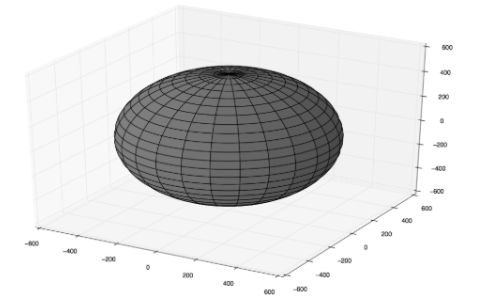
\includegraphics{Asset/image11.png}

}

\caption{Gambar 2.6. Ilustrasi Matplotlib}

\end{figure}

Instalasi Matplotlib

\begin{Shaded}
\begin{Highlighting}[]
\OperatorTok{!}\NormalTok{ pip install matplotlib}
\end{Highlighting}
\end{Shaded}

Menggunakan Library Matplotlib

\begin{Shaded}
\begin{Highlighting}[]
\ImportTok{import}\NormalTok{ matplotlib}
\end{Highlighting}
\end{Shaded}

\hypertarget{python-image-library-pil}{%
\subsection*{Python Image Library
(PIL)}\label{python-image-library-pil}}
\addcontentsline{toc}{subsection}{Python Image Library (PIL)}

Python Imaging Library (PIL) adalah modul untuk membaca, menulis, dan
memproses file gambar. Modul ini mendukung sebagian besar format gambar
umum seperti JPEG, PNG, TIFF, dll. \textbf{Namun, sejak versi Python
3.0, PIL tidak lagi dikembangkan dan digantikan oleh library yang
disebut Pillow.}\\
Installasi Pillow

\begin{Shaded}
\begin{Highlighting}[]
\OperatorTok{!}\NormalTok{ pip install Pillow}
\end{Highlighting}
\end{Shaded}

Menggunakan Library Pillow

\begin{Shaded}
\begin{Highlighting}[]
\ImportTok{from}\NormalTok{ PIL }\ImportTok{import}\NormalTok{ image}
\end{Highlighting}
\end{Shaded}

\hypertarget{scikits}{%
\subsection*{Scikits}\label{scikits}}
\addcontentsline{toc}{subsection}{Scikits}

Scikits adalah singkatan dari scipy toolkits. Ini adalah paket tambahan
yang dapat digunakan bersama dengan alat-alat scipy. Sebuah algoritma
diprogram dalam scikits jika:

\begin{itemize}
\tightlist
\item
  Algoritma tersebut masih dalam pengembangan dan belum siap untuk
  digunakan secara luas dalam scipy.\\
\item
  Paket tersebut memiliki lisensi yang tidak kompatibel dengan scipy.\\
\item
  Scipy adalah paket ilmiah umum dalam bahasa Python. Oleh karena itu,
  dirancang agar dapat diterapkan dalam berbagai bidang. Jika sebuah
  paket dianggap khusus untuk bidang tertentu, maka paket tersebut tetap
  menjadi bagian dari scikits.\\
  Scikits terdiri dari modul-modul dari berbagai bidang seperti ilmu
  lingkungan, analisis statistik, pemrosesan gambar, rekayasa mikrowave,
  pemrosesan audio, masalah nilai batas, penyesuaian kurva, komputasi
  kuantum, dll.
\end{itemize}

Dalam buku ini, kita akan fokus hanya pada rutinitas pemrosesan gambar
dalam scikits yang disebut scikit-image. Rutinitas scikit-image ini
berisi algoritma-algoritma untuk input/output, morfologi, deteksi dan
analisis objek, dll.

Installasi Skimage

\begin{Shaded}
\begin{Highlighting}[]
\OperatorTok{!}\NormalTok{ pip install scikit}\OperatorTok{{-}}\NormalTok{image}
\end{Highlighting}
\end{Shaded}

Penggunaan Library Skimage

\begin{Shaded}
\begin{Highlighting}[]
\ImportTok{from}\NormalTok{ skimage }\ImportTok{import}\NormalTok{ filters}
\ImportTok{import}\NormalTok{ skimage.filters }\ImportTok{as}\NormalTok{ fi}
\end{Highlighting}
\end{Shaded}

Pada perintah pertama, hanya submodul filters yang dimuat. Pada perintah
kedua, modul filters dimuat sebagai fi.

\hypertarget{modul-python-opencv}{%
\subsection*{Modul Python OpenCV}\label{modul-python-opencv}}
\addcontentsline{toc}{subsection}{Modul Python OpenCV}

Open Source Computer Vision Library (OpenCV) {[}Ope20a{]} adalah
perpustakaan perangkat lunak untuk pemrosesan gambar, penglihatan
komputer, dan pembelajaran mesin. Ini memiliki lebih dari 2000 algoritma
untuk memproses data gambar. OpenCV memiliki basis pengguna yang besar
dan digunakan secara luas di lembaga akademik, organisasi komersial, dan
lembaga pemerintah. Perpustakaan ini menyediakan ikatan (binding) untuk
bahasa pemrograman umum seperti C, C++, Python, dll.

Installasi Opencv

\begin{Shaded}
\begin{Highlighting}[]
\OperatorTok{!}\NormalTok{ pip install opencv}\OperatorTok{{-}}\NormalTok{python}
\end{Highlighting}
\end{Shaded}

Menggunakan Library OpenCV

\begin{Shaded}
\begin{Highlighting}[]
\ImportTok{import}\NormalTok{ cv2}
\end{Highlighting}
\end{Shaded}

\hypertarget{dasar-dasar-image-processing}{%
\chapter*{3 Dasar-dasar Image
Processing}\label{dasar-dasar-image-processing}}
\addcontentsline{toc}{chapter}{3 Dasar-dasar Image Processing}

\markboth{3 Dasar-dasar Image Processing}{3 Dasar-dasar Image
Processing}

Pada Modul ini membahas dasar-dasar image processing membahas konsep
dasar dalam Image Processing, yang merupakan bagian penting dari
Computer Vision. Anda akan mempelajari definisi Image Processing,
aplikasinya dalam kehidupan sehari-hari, dan perbedaannya dengan
Computer Vision. Selain itu, Anda akan memahami konsep dasar citra
digital, termasuk operasi transformasi, filtering, dan edge detection.
Penggunaan Python untuk Image Processing juga akan diajarkan, termasuk
instalasi dan penggunaan library seperti OpenCV, TensorFlow, dan Keras.
Modul ini juga mencakup latihan praktik untuk mengaplikasikan konsep dan
teknik yang telah dipelajari. Dengan menyelesaikan Modul 2, Anda akan
memiliki pemahaman yang kuat tentang dasar-dasar Image Processing dan
keterampilan untuk mengimplementasikannya menggunakan Python.

\url{https://youtu.be/LRP4WWElvnQ?feature=shared}

\hypertarget{a.-pengenalan-image-processing}{%
\section*{A. Pengenalan Image
Processing}\label{a.-pengenalan-image-processing}}
\addcontentsline{toc}{section}{A. Pengenalan Image Processing}

\markright{A. Pengenalan Image Processing}

Manusia mengandalkan penglihatan mereka untuk tugas-tugas mulai dari
pengenalan pola hingga naluri bertahan hidup. Kemampuan manusia untuk
melakukan analisis yang kompleks dan rinci terhadap suatu karya seni
berdasarkan input visual adalah sesuatu yang luar biasa. Namun, sejauh
mana manusia dapat melakukan apa yang komputer lakukan dengan sangat
cepat masih perlu diteliti.\\
Kebutuhan untuk mengekstrak informasi dari citra dan menginterpretasikan
isinya telah menjadi salah satu faktor pendorong dalam perkembangan
pemrosesan citra dan visi komputer selama beberapa dekade terakhir.
Aplikasi pemrosesan citra meliputi berbagai aktivitas manusia, antara
lain:

\begin{itemize}
\item
  Aplikasi medis: Modalitas pencitraan diagnostik seperti radiografi
  digital, PET (tomografi emisi positron), CT (tomografi aksial
  komputer), MRI (pemindaian resonansi magnetik), dan fMRI (pemindaian
  resonansi magnetik fungsional) telah diadopsi secara luas oleh
  komunitas medis.\\
\item
  Aplikasi industri: Sistem pemrosesan citra telah berhasil digunakan
  dalam sistem manufaktur untuk berbagai tugas, seperti sistem keamanan,
  kontrol kualitas, dan pengendalian kendaraan berpemandu otomatis
  (AGVs).\\
\item
  Aplikasi militer: Skenario yang paling menantang dan kritis dalam hal
  kinerja pemrosesan citra adalah untuk mendukung tugas militer, mulai
  dari deteksi tentara atau kendaraan hingga panduan rudal dan
  pengenalan objek dan tugas pengintaian menggunakan kendaraan udara tak
  berawak atau UAV. Selain itu, aplikasi militer sering kali membutuhkan
  penggunaan sensor pendeteksi yang khusus, seperti kamera jarak dan
  kamera inframerah yang melihat ke depan.
\item
  Penegakan hukum dan keamanan: Pengawasan adalah salah satu bidang yang
  banyak diteliti dalam komunitas pemrosesan video.\\
\item
  Teknologi biometrik (seperti pengenalan sidik jari, wajah, iris, dan
  telapak tangan) telah menjadi subjek penelitian dalam pemrosesan citra
  selama lebih dari satu dekade dan kini telah digunakan secara
  komersial.\\
\item
  Elektronik konsumen: Kamera digital dan camcorder, dengan kemampuan
  pemrosesan yang canggih, telah membuat film dan teknologi pita analog
  menjadi usang. Paket perangkat lunak untuk meningkatkan, mengedit,
  mengatur, dan mempublikasikan citra dan video telah maju pesat dalam
  kompleksitasnya sambil tetap menjaga antarmuka yang ramah pengguna. TV
  berdefinisi tinggi, monitor, pemutar DVD, dan pemutar video pribadi
  (PVR) semakin meningkat popularitasnya karena harga yang terjangkau.
  Perkembangan jaringan dan distribusi juga telah berhasil membuat
  terobosan dalam perangkat lain, seperti personal digital assistants
  (PDA), ponsel, dan pemutar musik portabel (MP3).\\
\item
  Internet, khususnya World Wide Web: Ada banyak informasi visual yang
  tersedia di web. Kolaborasi dalam mengunggah, berbagi, dan memberi
  anotasi (tagging) pada video semakin populer. Menemukan dan mengambil
  citra dan video di web berdasarkan isinya tetap menjadi tantangan
  terbuka dalam penelitian.
\end{itemize}

\hypertarget{b.-konsep-dasar-image-processing}{%
\section*{B. Konsep Dasar Image
Processing}\label{b.-konsep-dasar-image-processing}}
\addcontentsline{toc}{section}{B. Konsep Dasar Image Processing}

\markright{B. Konsep Dasar Image Processing}

Sebuah gambar digital merupakan larik 2D dari angka-angka yang mewakili
versi sampel dari sebuah gambar. Gambar didefinisikan dalam bentuk grid,
setiap lokasi grid disebut piksel. Sebuah gambar direpresentasikan oleh
grid yang terbatas dan setiap nilai intensitas direpresentasikan oleh
sejumlah bit yang terbatas. M x N pada gambar f(x, y) didefinisikan
sebagai:

\begin{figure}

\begin{minipage}[t]{0.50\linewidth}

{\centering 

\raisebox{-\height}{

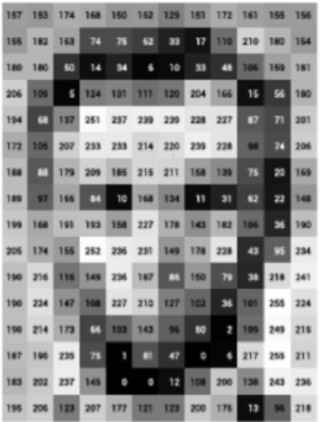
\includegraphics{Asset/image119.jpg}

}

\caption{Gambar 3.1. Perhitungan Resolusi Citra}

}

\end{minipage}%
%
\begin{minipage}[t]{0.50\linewidth}

{\centering 

\raisebox{-\height}{

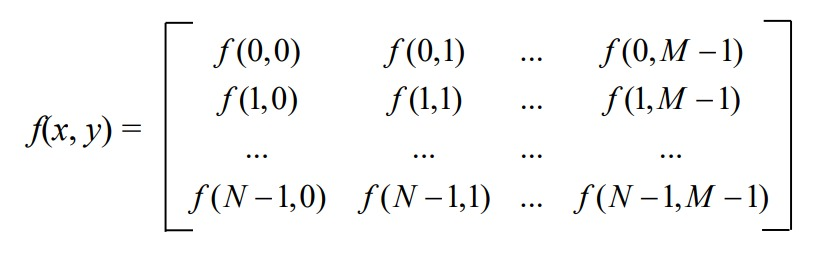
\includegraphics{Asset/image120.jpg}

}

}

\end{minipage}%

\end{figure}

Dalam representasi ini, digunakan {[}0, L --- 1{]} jumlah tingkat
intensitas untuk mewakili semua nilai piksel grayscale, dan k jumlah bit
digunakan untuk mewakili setiap tingkat intensitas, yaitu, L = 2k. Jadi,
jumlah bit yang diperlukan untuk menyimpan gambar M x N adalah M x N x
k. Kecerahan sebuah gambar merujuk pada tingkat keseluruhan cahaya atau
kegelapan gambar, sementara kontras adalah perbedaan antara intensitas
piksel maksimum dan minimum dalam sebuah gambar. Kecerahan dapat
meningkat atau dikurangi dengan penambahan atau pengurangan sederhana
pada nilai piksel.\\
Sebuah gambar biner direpresentasikan oleh hanya satu bit. Di sisi lain,
gambar grayscale direpresentasikan oleh 8 bit. Sebuah gambar raster
adalah kumpulan titik-titik, yang disebut piksel. Sebuah gambar vektor
adalah kumpulan garis dan kurva yang terhubung, dan digunakan untuk
menghasilkan objek.\\
Sebuah gambar adalah fungsi f, dari ruang R2 ke ruang R. Sebuah gambar
direpresentasikan oleh f(x.y'), dan itu menunjukkan intensitas di posisi
(x,y). Oleh karena itu, sebuah gambar hanya didefinisikan pada sebuah
persegi panjang, dengan rentang yang terbatas, yaitu,\\
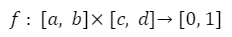
\includegraphics{Asset/image1111.png}\\
Gambar berwarna memiliki komponen Merah (R), Hijau (G), dan Biru (B).
Masing-masing dari ketiga komponen R, G, B biasanya direpresentasikan
oleh 8 bit, dan oleh karena itu dibutuhkan 24-bit untuk sebuah gambar
berwarna. Tiga warna primer ini dicampur dalam proporsi yang berbeda
untuk mendapatkan warna-warna yang berbeda. Untuk berbagai aplikasi
pengolahan gambar, format RGB, HIS, YIQ, YCbCr, dll. digunakan. Sebuah
gambar berwarna adalah fungsi tiga komponen, yang merupakan fungsi
``nilai-vektor'', dan direpresentasikan sebagai berikut:\\
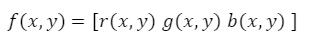
\includegraphics{Asset/image1112.png}

Gambar terindeks memiliki peta warna yang terkait, yang merupakan daftar
dari semua warna yang digunakan dalam gambar tersebut. Contoh dari
format ini adalah gambar PNG dan GIF. Jadi, berbagai jenis gambar
digital dapat dijelaskan sebagai berikut.

\begin{itemize}
\tightlist
\item
  Gambar biner - 1 bit/pixel
\item
  Gambar grayscale - 8 bit/pixel
\item
  Gambar warna asli atau RGB - 24 bit/pixel
\item
  Gambar terindeks - 8 bit/pixel
\end{itemize}

Resolusi spasial sebuah gambar mendefinisikan jumlah piksel yang
digunakan untuk mencakup ruang visual yang ditangkap oleh gambar
tersebut. Resolusi intensitas sebuah gambar bergantung pada jumlah bit
yang digunakan untuk mewakili nilai intensitas yang berbeda. Jumlah
gambar atau frame video yang ditangkap oleh kamera dalam waktu tertentu
menentukan resolusi temporal. Kurangnya jumlah tingkat intensitas
(resolusi intensitas rendah) di area halus sebuah gambar menghasilkan
``efek kontur palsu'', yaitu, menciptakan tepi atau garis palsu di mana
aslinya tidak ada. Juga ``efek kotak-kotak'' terjadi ketika resolusi
spasial sebuah gambar sangat rendah.\\
Pengolahan gambar digital berurusan dengan manipulasi dan analisis
gambar digital oleh sistem digital. Sebuah operasi pengolahan gambar
biasanya mendefinisikan gambar baru g dalam hal gambar masukan
f.~Seperti yang ditunjukkan dalam Gambar 3.6, kita dapat mengubah
rentang f menjadi g(x, y) = t(f(x,y)), atau kita dapat mengubah domain f
menjadi g(x,y) = f(tx(x,y),ty(x,y)). Nilai piksel dimodifikasi dalam
transformasi pertama (Gambar 3.5); sedangkan posisi piksel spasial
berubah dalam transformasi kedua (Gambar 3.6). Domain sebuah gambar
dapat diubah dengan memutar dan menyesuaikan skala gambar seperti yang
diilustrasikan dalam Gambar 3.6.

\begin{figure}

{\centering 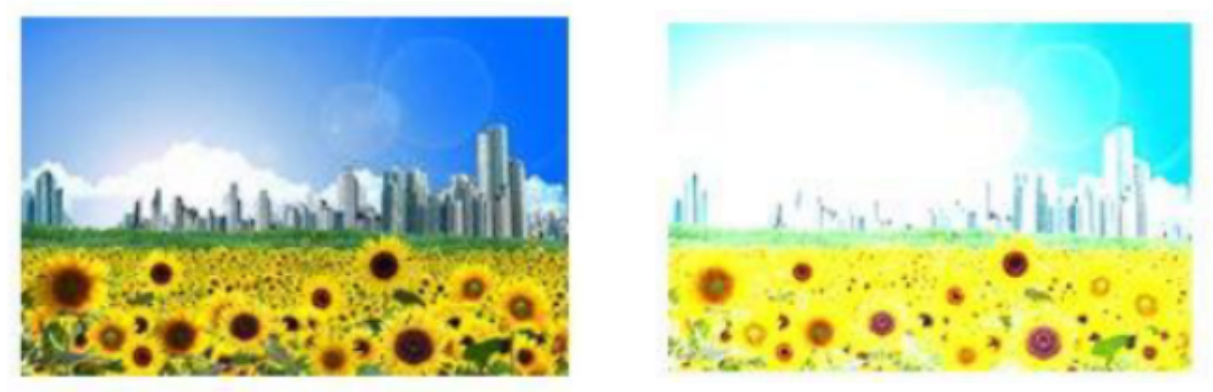
\includegraphics{Asset/image1113.png}

}

\caption{Gambar 3.5. Mengubah Rentang Gambar}

\end{figure}

\begin{figure}

{\centering 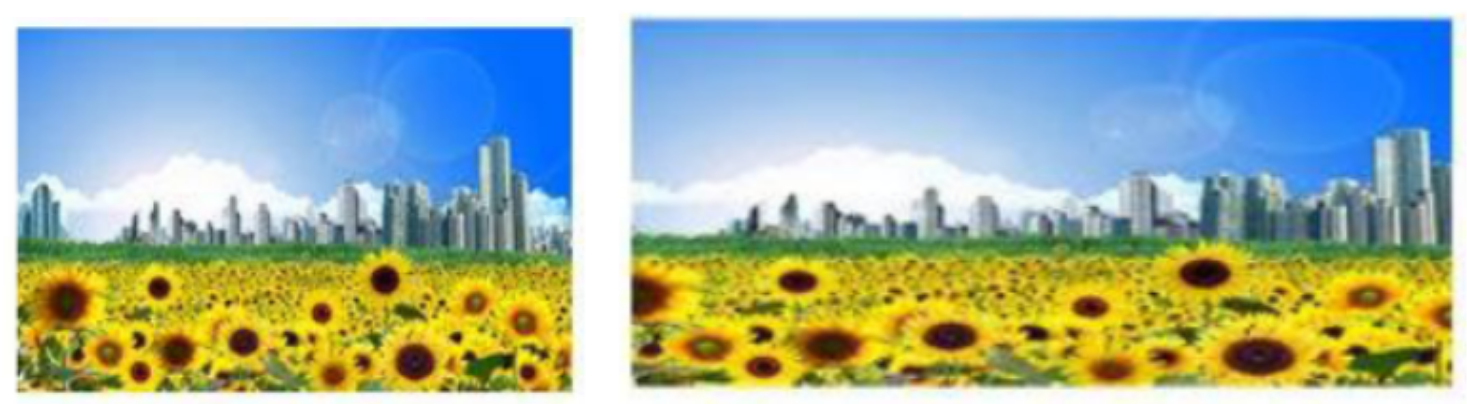
\includegraphics{Asset/image1114.png}

}

\caption{Gambar 3.6. Mengubah Domain dari Suatu Gambar}

\end{figure}

\hypertarget{c.-python-untuk-image-processing}{%
\section*{C. Python Untuk Image
Processing}\label{c.-python-untuk-image-processing}}
\addcontentsline{toc}{section}{C. Python Untuk Image Processing}

\markright{C. Python Untuk Image Processing}

Dalam tutorial ini, Anda akan menemukan fungsi dasar untuk memuat,
memanipulasi, dan menampilkan gambar. Informasi utama dari gambar akan
diperoleh, seperti ukuran, jumlah saluran, kelas penyimpanan, dan
lain-lain. Setelah itu, Anda akan dapat melakukan filter klasik pertama
Anda.\\
Proses yang berbeda akan dilakukan pada gambar-gambar berikut ini:

\begin{figure}

{\centering 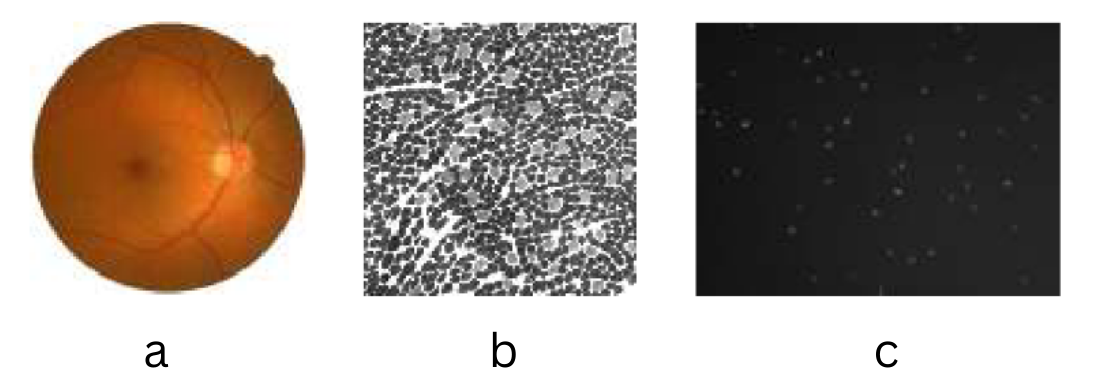
\includegraphics{Asset/image1115.png}

}

\caption{Gambar 3.7. (a)Retina Vessel, (b)Muscle Cells, (c)Cornea Cells}

\end{figure}

\hypertarget{spatial-filter}{%
\subsection*{Spatial Filter}\label{spatial-filter}}
\addcontentsline{toc}{subsection}{Spatial Filter}

\hypertarget{filtering}{%
\subsubsection*{Filtering}\label{filtering}}
\addcontentsline{toc}{subsubsection}{Filtering}

Seperti halnya filter air yang menghilangkan kotoran, filter pemrosesan
gambar menghapus fitur yang tidak diinginkan (seperti noise) dari sebuah
gambar. Setiap filter memiliki utilitas khusus dan dirancang untuk
menghilangkan jenis noise tertentu atau meningkatkan aspek tertentu dari
gambar. Kami akan membahas banyak filter beserta tujuan dan efek mereka
pada gambar.\\
Untuk melakukan filtering, digunakan filter atau masker. Biasanya, ini
berupa jendela persegi dua dimensi yang bergerak melintasi gambar hanya
mempengaruhi satu piksel pada satu waktu. Setiap angka dalam filter
dikenal sebagai koefisien. Koefisien dalam filter menentukan efek dari
filter dan akibatnya gambar keluaran. Mari kita pertimbangkan filter
3x3, F, yang diberikan dalam Tabel 3.1.

\begin{figure}

{\centering 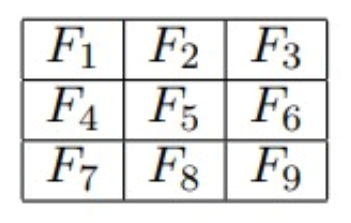
\includegraphics[width=0.3\textwidth,height=\textheight]{Asset/image1116.png}

}

\caption{Tabel 3.1. Filter 3x3}

\end{figure}

Jika (i, j) adalah piksel dalam gambar, maka sub-gambar di sekitar (i,
j) dengan dimensi yang sama dengan filter akan dipertimbangkan untuk
filtering. Pusat filter ditempatkan agar tumpang tindih dengan (i, j).
Piksel-piksel dalam sub-gambar dikalikan dengan koefisien yang sesuai
dalam filter. Hal ini menghasilkan matriks dengan ukuran yang sama
dengan filter. Matriks ini disederhanakan menggunakan persamaan
matematika untuk mendapatkan satu nilai yang akan menggantikan nilai
piksel pada (i, j) dalam gambar. Persamaan matematika yang tepat
tergantung pada jenis filter. Misalnya, dalam kasus filter rata-rata,
nilai F adalah -7, di mana N adalah jumlah elemen dalam filter. Gambar
yang difilter diperoleh dengan mengulangi proses penempatan filter pada
setiap piksel dalam gambar, memperoleh satu nilai, dan menggantikan
nilai piksel dalam gambar asli. Proses ini memindahkan jendela filter
melintasi gambar disebut konvolusi dalam domain spasial.

Mari kita pertimbangkan sub-gambar berikut dari gambar I, yang berpusat
pada (i, j).

\begin{figure}

{\centering 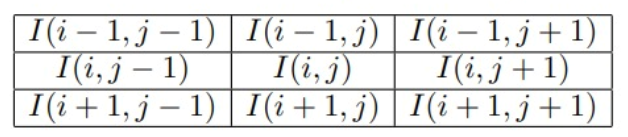
\includegraphics[width=0.7\textwidth,height=\textheight]{Asset/image1117.png}

}

\caption{Gambar 3.8. Konvolusi filter}

\end{figure}

Konvolusi filter yang diberikan dalam Gambar 3.8 dengan sub-gambar dalam
Gambar 3.9 diberikan sebagai berikut:

\begin{figure}

{\centering 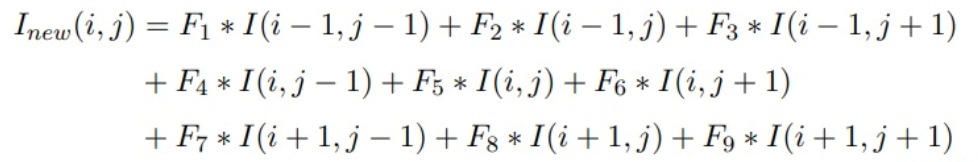
\includegraphics{Asset/image1118.png}

}

\caption{Gambar 3.9. Rumus Konvolusi filter}

\end{figure}

Di mana Inew(i, j) adalah nilai keluaran pada lokasi (i, j). Proses ini
harus diulang untuk setiap piksel dalam gambar. Karena filter memainkan
peran penting dalam proses konvolusi, filter juga dikenal sebagai kernel
konvolusi.

Operasi konvolusi harus dilakukan pada setiap piksel dalam gambar,
termasuk piksel di batas gambar. Ketika filter ditempatkan pada piksel
batas, sebagian filter akan berada di luar batas gambar. Karena nilai
piksel di luar batas tidak ada, nilai-nilai baru harus dibuat sebelum
konvolusi. Proses ini untuk menciptakan nilai piksel di luar batas
disebut padding. Piksel yang dipadatkan dapat diasumsikan nol atau nilai
tetap. Pilihan padding lainnya seperti nearest neighbor atau reflect
menciptakan piksel yang dipadatkan menggunakan nilai piksel dalam
gambar. Dalam kasus nol, piksel yang dipadatkan semua bernilai nol.
Dalam kasus konstan, piksel yang dipadatkan mengambil nilai spesifik.
Dalam kasus reflect, piksel yang dipadatkan mengambil nilai dari baris
atau kolom terakhir. Piksel yang dipadatkan hanya dipertimbangkan untuk
konvolusi dan akan dibuang setelah konvolusi.

Mari kita pertimbangkan contoh untuk menunjukkan berbagai pilihan
padding. Gambar 3.10 adalah gambar input berukuran 7x7 yang akan
dikonvolusi menggunakan filter 3x5 dengan pusat filter di (1,2). Untuk
memasukkan piksel batas dalam konvolusi, kita memasukkan gambar dengan
satu baris di atas dan satu baris di bawah serta dua kolom di sebelah
kiri dan dua kolom di sebelah kanan. Secara umum, ukuran filter
menentukan jumlah baris dan kolom yang akan dipadatkan ke gambar.

\begin{itemize}
\tightlist
\item
  Padding dengan nol: Semua piksel yang dipadatkan diberi nilai nol
  (Gambar 3.11).
\item
  Padding dengan konstanta: Nilai konstan 5 digunakan untuk semua piksel
  yang dipadatkan (Gambar 3.12). Nilai konstan dapat dipilih berdasarkan
  jenis gambar yang sedang diproses.
\item
  Nearest neighbor: Nilai dari baris atau kolom terakhir (Gambar 3.13)
  digunakan untuk padding.
\item
  Reflect: Nilai dari baris atau kolom terakhir (Gambar 3.14)
  dipantulkan melintasi batas gambar.
\item
  Wrap: Dalam opsi wrap seperti yang ditunjukkan dalam Gambar 3.15,
  baris pertama (atau kolom) setelah batas mengambil nilai yang sama
  dengan baris pertama (atau kolom) dalam gambar, dan seterusnya.
\end{itemize}

\begin{figure}

\begin{minipage}[t]{0.50\linewidth}

{\centering 

\raisebox{-\height}{

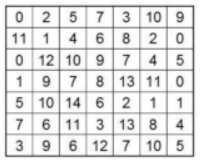
\includegraphics{Asset/image1119.png}

}

\caption{Gambar 3.10. 7 x 7 input citra}

}

\end{minipage}%
%
\begin{minipage}[t]{0.50\linewidth}

{\centering 

\raisebox{-\height}{

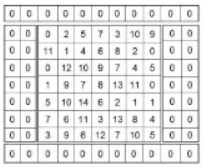
\includegraphics{Asset/image1120.png}

}

\caption{Gambar 3.11. Padding dengan kosong}

}

\end{minipage}%
\newline
\begin{minipage}[t]{0.50\linewidth}

{\centering 

\raisebox{-\height}{

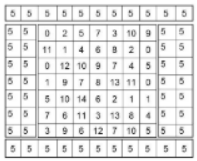
\includegraphics{Asset/image1121.png}

}

\caption{Gambar 3.12. Padding dengan nilai konstant}

}

\end{minipage}%
%
\begin{minipage}[t]{0.50\linewidth}

{\centering 

\raisebox{-\height}{

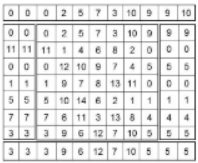
\includegraphics{Asset/image1122.png}

}

\caption{Gambar 3.13. Padding dengan nearest neighbors}

}

\end{minipage}%
\newline
\begin{minipage}[t]{0.50\linewidth}

{\centering 

\raisebox{-\height}{

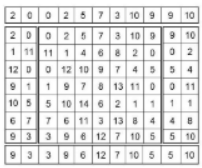
\includegraphics{Asset/image1123.png}

}

\caption{Gambar 3.14. Padding dengan nearest neighbors}

}

\end{minipage}%
%
\begin{minipage}[t]{0.50\linewidth}

{\centering 

\raisebox{-\height}{

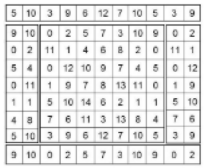
\includegraphics{Asset/image1124.png}

}

\caption{Gambar 3.15. Padding dengan wrap option}

}

\end{minipage}%

\end{figure}

\hypertarget{shape-detection-filter}{%
\paragraph*{\texorpdfstring{\textbf{Shape Detection
Filter}}{Shape Detection Filter}}\label{shape-detection-filter}}
\addcontentsline{toc}{paragraph}{\textbf{Shape Detection Filter}}

\textbf{Frangi Filter}

Kegunaan dari Filter Frangi {[}AFFV98{]} yaitu mendeteksi objek yang
mirip dengan pembuluh darah pada sebuah gambar. Sebelum membahas
matematika dibaliknya, pembahasan akan dimulai dengan ide fundamental
dari Frangi itu sendiri. Pada gambar 3.16 berisi dua objek, salah satu
objek memanjang ke satu arah, akan tetapi tidak ke arah lainnya,
sedangkan objek kedua berbentuk persegi. Secara proporsional, panah
ortogonal digambar dimana panjangnya sepanjang suatu arah tertentu.
Dengan mendapatkan nilai eigen dari kedua objek tersebut, maka kita
dapat mengukur perbedaan geometri kualitatif ini. Objek yang memanjang,
nilai eigennya akan lebih besar pada arah panah yang lebih panjang serta
lebih kecil pada arah panah yang lebih pendek. Sedangkan objek persegi,
nilai eigen pada arah panah yang lebih panjang serupa dengan nilai eigen
pada arah panah yang lebih pendek. Filter Frangi menggunakan gambar
turunan kedua (Hessian) sebagai dasar perhitungan nilai eigen, bukan
menggunakan gambar asli. Turunan kedua atau Hessian merupakan
representasi matematis dari perubahan intensitas piksel dalam gambar.
Dengan menggunakan gambar turunan kedua, Filter Frangi dapat
mengidentifikasi dan menghitung nilai eigen yang mencerminkan
karakteristik objek mirip pembuluh darah dengan lebih baik daripada
menggunakan gambar asli. Maka dari itu, penggunaan gambar turunan kedua
memungkinkan Filter Frangi untuk memperoleh informasi yang lebih relevan
dan memperbaiki kemampuan deteksi objek pembuluh darah.

\begin{figure}

{\centering 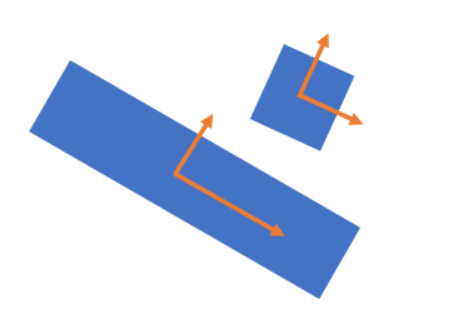
\includegraphics{Asset/image1125.png}

}

\caption{Gambar 3.16. Ilustrasi Frangi Filter}

\end{figure}

Noise yang disebabkan oleh turunan dapat dikurangi menggunakan konvolusi
dimana gambar akan dihaluskan. Pada konteks umum, metode yang digunakan
adalah penghalusan Gaussian. Penghalusan Gaussian merupakan teknik
pengolahan citra yang menggunakan filter Gaussian untuk mengurangi nois
dan menyamarkan detail tajam pada gambar. Dalam buku ini akan
ditunjukkan bahwa mencari turunan dari gambar yang dihaluskan dengan
konvolusi Gaussian setara dengan mencari turunan dari Gaussian yang
dikonvolusikan dengan gambar. Selanjutnya, kami akan menghitung turunan
kedua dari Gaussian dengan menggunakan rumus berikut ini, di mana gσ
merupakan fungsi Gaussian.

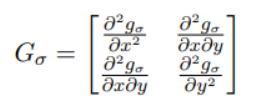
\includegraphics{Asset/image1126.png}

Selanjutnya, menentukan turunan kedua lokal (Hessian) dan nilai
eigen-nya. Untuk gambar 2D, setiap koordinat piksel akan memiliki dua
nilai eigen (λ1 dan λ2). Kemudian, nilai eigen diurutkan dalam urutan
meningkat. Sebuah piksel dianggap sebagai bagian dari struktur tabung
atau mirip pembuluh darah jika λ1 ≈ 0 dan \textbar λ2\textbar{}
\textgreater{} \textbar λ1\textbar. Sedangkan untuk citra 3D, setiap
koordinat voxel akan memiliki tiga nilai eigen (λ1, λ2, dan λ3). Nilai
eigen tersebut kemudian diurutkan dalam urutan meningkat. Sebuah voxel
dianggap sebagai bagian dari struktur tabung atau mirip pembuluh darah
jika λ1 ≈ 0 sementara λ2 dan λ3 memiliki nilai absolut yang tinggi yang
hampir sama dan memiliki tanda yang sama. Pembuluh yang terlihat terang
akan memiliki nilai positif untuk λ2 dan λ3, sedangkan pembuluh yang
lebih gelap akan memiliki nilai negatif untuk λ2 dan λ3.

\hypertarget{rangkuman}{%
\section*{Rangkuman}\label{rangkuman}}
\addcontentsline{toc}{section}{Rangkuman}

\markright{Rangkuman}

\begin{itemize}
\tightlist
\item
  Filter rata-rata menghaluskan gambar sambil mengaburkan bagian tepi
  dalam gambar.
\item
  Filter median efektif dalam menghilangkan noise salt-and-pepper.
\item
  Filter turunan pertama yang paling banyak digunakan adalah Sobel,
  Prewitt, dan Canny.
\item
  Baik Laplacian maupun LoG adalah filter turunan kedua yang populer.
  Laplacian sangat sensitif terhadap noise. Pada LoG, Gaussian
  menghaluskan gambar sehingga noise dari Laplacian dapat dikompensasi.
  Namun, LoG mengalami efek `spaghetti'. (*Efek `spaghetti' merujuk pada
  hasil filter LoG yang menghasilkan garis-garis tipis seperti spageti
  yang melintang di sekitar tepi objek dalam gambar. Efek ini terjadi
  karena penggunaan kernel LoG yang besar atau parameter yang tidak
  sesuai, yang mengakibatkan respons yang berlebihan dan menciptakan
  garis-garis halus yang terlalu banyak pada tepi objek dalam gambar.
  Hasilnya adalah gambar yang terdistorsi dan sulit diinterpretasikan
  dengan jelas)
\item
  Filter Frangi digunakan untuk mendeteksi struktur yang mirip dengan
  pembuluh darah.
\end{itemize}

\hypertarget{feature-extraction-and-matching}{%
\chapter*{4 Feature Extraction and
Matching}\label{feature-extraction-and-matching}}
\addcontentsline{toc}{chapter}{4 Feature Extraction and Matching}

\markboth{4 Feature Extraction and Matching}{4 Feature Extraction and
Matching}

\hypertarget{a.-pengenalan-feature-extraction-and-matching}{%
\section*{A. Pengenalan Feature Extraction and
Matching}\label{a.-pengenalan-feature-extraction-and-matching}}
\addcontentsline{toc}{section}{A. Pengenalan Feature Extraction and
Matching}

\markright{A. Pengenalan Feature Extraction and Matching}

Ekstraksi dan Pencocokan Fitur adalah tugas penting dalam visi komputer,
seperti struktur dari gerak, pengambilan gambar, dan deteksi objek.\\
Fitur adalah bagian dari informasi yang relevan untuk menyelesaikan
tugas komputasi yang terkait dengan aplikasi tertentu. Fitur mungkin
struktur tertentu dalam gambar seperti titik, tepi atau objek. Fitur
mungkin juga merupakan hasil dari operasi lingkungan umum atau deteksi
fitur yang diterapkan pada gambar. Fitur dapat diklasifikasikan menjadi
dua kategori utama:

\begin{itemize}
\tightlist
\item
  Fitur yang ada di lokasi tertentu dari gambar, seperti puncak gunung,
  sudut bangunan, pintu masuk, atau petak salju yang berbentuk menarik.
  Jenis fitur yang dilokalkan ini sering disebut fitur titik kunci (atau
  bahkan sudut) dan sering digambarkan dengan tampilan tambalan piksel
  yang mengelilingi lokasi titik.\\
\item
  Fitur yang dapat dicocokkan berdasarkan orientasi dan kenampakan
  lokalnya (profil tepi) disebut tepi dan juga dapat menjadi indikator
  yang baik untuk batasan objek dan kejadian oklusi dalam urutan citra.
\end{itemize}

Komponen utama Deteksi dan Pencocokan Fitur:\\
\textbf{Deteksi :} Identifikasi Feature Point.\\
\textbf{Deskripsi:} Penampilan lokal di sekitar setiap titik fitur
dijelaskan dalam beberapa cara yang (idealnya) tidak berubah di bawah
perubahan iluminasi, translasi, skala, dan rotasi dalam bidang. Kami
biasanya berakhir dengan vektor deskriptor untuk setiap titik fitur.\\
\textbf{Pencocokan:} Deskriptor dibandingkan di seluruh gambar, untuk
mengidentifikasi fitur serupa. Untuk dua gambar kita mungkin mendapatkan
satu set pasangan ( Xi, Yi ) ↔ ( Xi', Yi' ), di mana ( Xi, Yi ) adalah
fitur dalam satu gambar dan ( Xi', Yi' ) fitur pencocokannya di gambar
lainnya gambar.

\hypertarget{feature-descriptor}{%
\subsection*{Feature Descriptor}\label{feature-descriptor}}
\addcontentsline{toc}{subsection}{Feature Descriptor}

Deskriptor fitur adalah algoritme yang mengambil gambar dan menampilkan
deskriptor fitur/vektor fitur. Deskriptor fitur menyandikan informasi
menarik ke dalam rangkaian angka dan bertindak sebagai semacam ``sidik
jari'' numerik yang dapat digunakan untuk membedakan satu fitur dari
fitur lainnya.

\begin{figure}

{\centering 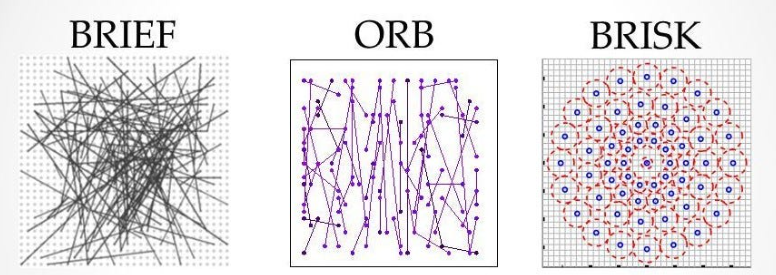
\includegraphics{Asset/image12.png}

}

\caption{Gambar 4.1. Macam-macam Feature Descriptor}

\end{figure}

Idealnya, informasi ini akan menjadi invarian di bawah transformasi
citra, sehingga kita dapat menemukan kembali fitur tersebut bahkan jika
citra diubah dalam beberapa cara. Setelah mendeteksi feature point, kami
melanjutkan untuk menghitung deskriptor untuk masing-masingnya.
Deskriptor dapat dikategorikan menjadi dua kelas:

\begin{itemize}
\tightlist
\item
  Deskriptor Lokal: Ini adalah representasi kompak dari lingkungan lokal
  suatu titik. Deskriptor lokal mencoba untuk menyerupai bentuk dan
  penampilan hanya di lingkungan lokal sekitar titik dan dengan demikian
  sangat cocok untuk merepresentasikannya dalam hal pencocokan.\\
\item
  Deskriptor Global : Deskriptor global menjelaskan keseluruhan gambar.
  Mereka umumnya tidak terlalu kuat karena perubahan sebagian gambar
  dapat menyebabkannya gagal karena akan memengaruhi deskriptor yang
  dihasilkan.\\
  Macam - macam Algoritma Descriptor :\\
\item
  SIFT(Scale Invariant Feature Transform)\\
\item
  SURF(Speed Up Robust Feature)\\
\item
  ORB(Oriented FAST and Rotate BRIEF)\\
\item
  BRISK(Binary Robust Invariant Scalable Keypoints)\\
\item
  BRIEF(Binary Robust Independent Elementary Feature)
\end{itemize}

\hypertarget{feature-matching}{%
\subsection*{Feature Matching}\label{feature-matching}}
\addcontentsline{toc}{subsection}{Feature Matching}

Pencocokan fitur atau umumnya pencocokan gambar, bagian dari banyak
aplikasi visi komputer seperti pendaftaran gambar, kalibrasi kamera dan
pengenalan objek, adalah tugas membangun korespondensi antara dua gambar
dari pemandangan/objek yang sama. Pendekatan umum untuk pencocokan citra
terdiri dari pendeteksian sekumpulan poin kepentingan yang masing-masing
terkait dengan deskriptor citra dari data citra. Setelah fitur dan
deskriptornya diekstraksi dari dua atau lebih gambar, langkah
selanjutnya adalah membuat beberapa pencocokan fitur awal antara
gambar-gambar ini.

\begin{figure}

{\centering 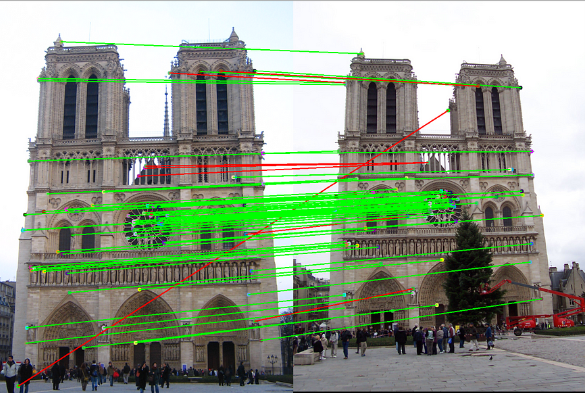
\includegraphics{Asset/image13.png}

}

\caption{Gambar 4.2. Pencocokan gambar}

\end{figure}

Secara umum, kinerja metode pencocokan berdasarkan interest point atau
feature point bergantung pada properti dari feature point yang
mendasarinya dan pilihan deskriptor gambar terkait. Dengan demikian,
detektor dan deskriptor yang sesuai untuk konten gambar harus digunakan
dalam aplikasi. Misalnya, jika gambar mengandung sel bakteri, detektor
blob harus digunakan daripada detektor sudut. Tapi, jika gambar tersebut
adalah pemandangan kota dari udara, detektor sudut cocok untuk menemukan
struktur buatan manusia. Selain itu, pemilihan detektor dan deskriptor
yang mengatasi degradasi citra sangatlah penting.\\
Macam - macam Algoritma Pencocokan:

\begin{itemize}
\tightlist
\item
  Brute-Force Matcher\\
\item
  FLANN(Fast Library for Aproximate Nearest Neighbors) Matcher
\end{itemize}

\hypertarget{template-matching}{%
\subsection*{Template Matching}\label{template-matching}}
\addcontentsline{toc}{subsection}{Template Matching}

\hypertarget{b.-hog-dan-sift}{%
\section*{B. HOG dan SIFT}\label{b.-hog-dan-sift}}
\addcontentsline{toc}{section}{B. HOG dan SIFT}

\markright{B. HOG dan SIFT}

\hypertarget{histogram-of-oriented-gradient-hog}{%
\subsection*{Histogram of Oriented Gradient
(HOG)}\label{histogram-of-oriented-gradient-hog}}
\addcontentsline{toc}{subsection}{Histogram of Oriented Gradient (HOG)}

Histogram of Oriented Gradients (HOG) adalah deskriptor fitur citra yang
dapat digunakan untuk deteksi objek {[}52{]}. Untuk mengekstrak fitur
ini, frekuensi orientasi gradien dalam bagian-bagian lokal citra
dihitung. Penampilan dan bentuk objek lokal dalam sebuah citra dapat
dijelaskan melalui distribusi gradien intensitas atau arah tepi.
Langkah-langkah berikut perlu diimplementasikan untuk mengekstrak fitur
HOG:

\begin{itemize}
\tightlist
\item
  Perhitungan gradien: Langkah pertama adalah menghitung gradien
  horizontal dan vertikal yang terpusat (Gx dan Gy) tanpa melakukan
  smoothing pada citra. Untuk tujuan ini, dapat digunakan operator Sobel
  atau operator deteksi tepi lainnya untuk mendapatkan gradien. Untuk
  citra berwarna, saluran warna yang memberikan magnitudo gradien
  tertinggi untuk setiap piksel dapat dipilih. Kemudian, magnitudo
  gradien dan orientasi gradien dihitung sebagai berikut:\\

  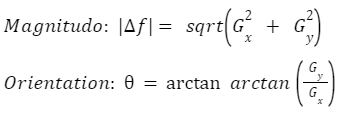
\includegraphics{Asset/image14.png}
\item
  Orientasi pengalamatan: Langkah kedua adalah pembuatan histogram sel.
  Untuk ini, orientasi gradien diquantisasi ke dalam bin. Setiap bin
  akan mendapatkan voting berdasarkan magnitudo gradien. Voting juga
  dapat diberi bobot dengan filter Gaussian untuk mengurangi bobot
  piksel-piksel di dekat tepi blok.
\end{itemize}

\begin{figure}

{\centering 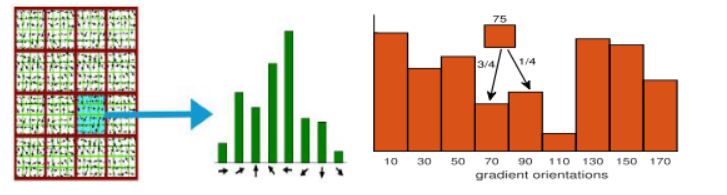
\includegraphics{Asset/image15.png}

}

\caption{Gambar 4.3. Histogram of oriented gradients: (a) cell histogram
and (b) orientation binning}

\end{figure}

Mari kita ambil contoh ekstraksi deskriptor HOG. Untuk ini, kita
menggunakan citra berukuran 64 x 128. Pertama, citra dibagi menjadi blok
16 x 16 dengan tumpang tindih 50\%. Jadi, totalnya akan ada 7 x 15 = 105
blok. Setiap blok harus terdiri dari 2 x 2 sel dengan ukuran 8x8 piksel.
Sekarang, orientasi gradien diquantisasi menjadi 9 bin. Di sini, voting
adalah magnitudo gradien. Sekarang, voting diinterpolasi secara bilinear
antara pusat bin yang berdekatan. Misalnya, misalkan orientasi adalah
75°. Kemudian, jarak antara pusat bin bin 70 dan bin 90 adalah 5° dan
15°, masing-masing. Oleh karena itu, rasio kepemilikan adalah 15/20 atau
3/4 dan 5/20 atau 1/4. Hal ini ditunjukkan secara diagramatik pada
Gambar 4.3. (a) dan (b). Histogram dari gradien yang diarahkan
ditunjukkan pada Gambar 4.3(a).

\begin{itemize}
\tightlist
\item
  Penggabungan blok deskriptor: Histogram sel kemudian digabungkan untuk
  membentuk vektor fitur seperti yang ditunjukkan pada Gambar 3.26. Pada
  contoh kita, histogram yang diperoleh dari blok yang tumpang tindih 2
  x 2 sel digabungkan menjadi vektor fitur 1-D dengan dimensi 105 x 2 x
  2 x 9 = 3780.\\
\item
  Normalisasi blok: Setiap blok dapat dinormalisasi dengan faktor
  normalisasi yang berbeda, seperti L2-norm, Zq-norm, Li-squared root
  norm, dll. Normalisasi blok membuat deskriptor invariant terhadap
  variasi pencahayaan dan fotometri.\\
\item
  Deskriptor final: Deskriptor HOG akhir dapat digunakan untuk
  pengenalan objek. Deskriptor ini merupakan fitur untuk algoritma
  pembelajaran mesin, seperti Support Vector Machine (SVM).\\

  \begin{figure}

  {\centering 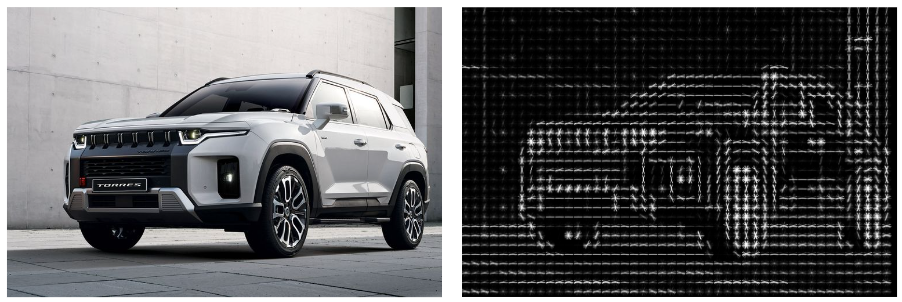
\includegraphics{Asset/image16.png}

  }

  \caption{Gambar 4.4. Hasil HOG}

  \end{figure}
\end{itemize}

\hypertarget{scale-invariant-feature-transform-sift}{%
\subsection*{Scale Invariant Feature Transform
(SIFT)}\label{scale-invariant-feature-transform-sift}}
\addcontentsline{toc}{subsection}{Scale Invariant Feature Transform
(SIFT)}

Transformasi fitur skala invarian (SIFT) adalah algoritma deteksi fitur
untuk mendeteksi dan menggambarkan fitur lokal pada gambar untuk
pengenalan objek. Detektor sudut Harris invarian terhadap translasi dan
rotasi, tetapi tidak terhadap skala. Namun, algoritma SIFT dapat
mendeteksi dan menggambarkan fitur lokal pada gambar. Fitur-fitur ini
invarian terhadap translasi, penskalaan, dan rotasi gambar, serta
sebagian invarian terhadap perubahan pencahayaan {[}55{]}. Fitur-fitur
gambar yang diekstraksi dari gambar latihan harus tetap terdeteksi
bahkan dengan perubahan skala gambar, noise, dan pencahayaan. Konsep
skala memainkan peran penting dalam analisis gambar. Dalam analisis
gambar, kita perlu mengekstraksi fitur gambar yang sesuai dengan
menganalisis struktur gambar yang berbeda. Struktur-struktur ini mungkin
ada pada skala yang berbeda. Jadi, jumlah informasi yang disampaikan
oleh struktur gambar tertentu tergantung pada skala. SIFT
mempertimbangkan masalah ini, yaitu fitur-fitur yang invariant terhadap
perubahan skala. Langkah-langkah utama dari algoritma SIFT adalah
sebagai berikut:

\begin{itemize}
\tightlist
\item
  Estimasi ekstremum skala-ruang: Ini sesuai dengan ekstremum DoG dan
  memastikan ekstraksi wilayah invarian skala. Tentukan lokasi perkiraan
  dan skala titik fitur yang menonjol (juga disebut ``keypoints'').\\
\item
  Lokalisasi dan penyaringan titik fitur: Perbaiki lokasi dan skala
  mereka, yaitu pilih titik fitur yang asli dan buang yang buruk.\\
\item
  Pemberian orientasi: Tentukan orientasi untuk setiap titik fitur,
  yaitu kurangi efek rotasi.\\
\item
  Membuat deskriptor: Menggunakan histogram deskriptor orientasi untuk
  setiap titik kunci.
\end{itemize}

Deskriptor ini dibuat dengan menghitung histogram orientasi untuk setiap
titik kunci. Deskriptor ini menangkap informasi gradien lokal di sekitar
titik kunci dan memberikan representasi yang khas dari wilayah lokal.
Langkah-langkah dalam membuat deskriptor adalah sebagai berikut:

\begin{itemize}
\tightlist
\item
  Bagi wilayah di sekitar titik kunci menjadi sub-wilayah atau bin yang
  lebih kecil.
\item
  Untuk setiap sub-wilayah, hitung magnitudo dan orientasi gradien
  piksel.
\item
  Tetapkan setiap piksel ke salah satu bin berdasarkan orientasi
  gradiennya.
\item
  Untuk setiap bin, akumulasikan magnitudo gradien dari piksel yang
  ditugaskan.
\item
  Buat histogram orientasi dengan mempertimbangkan magnitudo gradien
  yang terakumulasi sebagai bobot untuk setiap bin.
\item
  Normalisasi histogram untuk membuatnya invarian terhadap perubahan
  pencahayaan.
\item
  Deskriptor akhir terbentuk dengan menggabungkan histogram orientasi
  yang telah dinormalisasi.
\end{itemize}

Setelah deskriptor dihitung untuk semua titik kunci, mereka dapat
digunakan untuk berbagai aplikasi seperti pengenalan objek, penyatuan
gambar, dan pencarian gambar. Pemadanan titik kunci di gambar-gambar
yang berbeda berdasarkan deskriptornya memungkinkan pencocokan fitur
yang kuat melintasi perubahan skala, rotasi, dan pencahayaan.

Untuk mengimplementasikan algoritma SIFT dalam Python, dapat menggunakan
pustaka OpenCV. OpenCV menyediakan fungsi-fungsi untuk deteksi titik
kunci, perhitungan deskriptor, dan pencocokan fitur. Dapat merujuk pada
dokumentasi dan tutorial OpenCV untuk informasi detail tentang cara
menggunakan algoritma SIFT dalam Python.C. Feature Matching.\\

\begin{figure}

{\centering 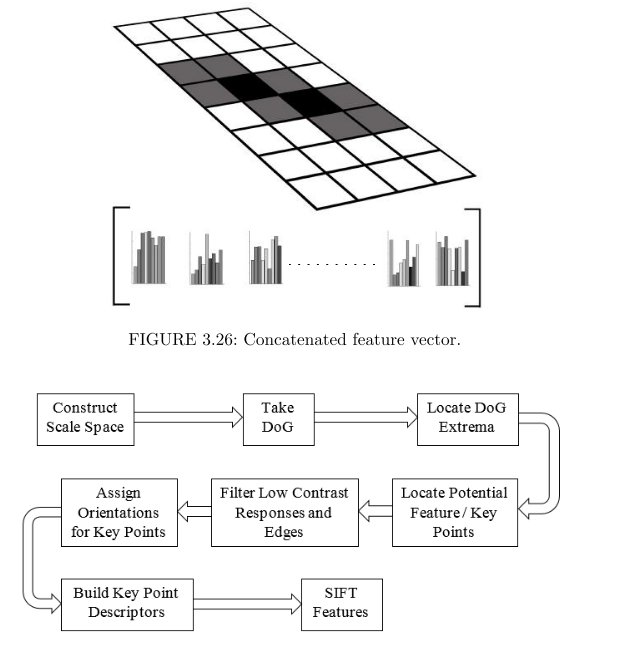
\includegraphics{Asset/image17.png}

}

\caption{Gambar 4.5. Implementasi Langkah algoritma SIFT}

\end{figure}

Gambar 4.5. menunjukkan semua langkah implementasi dari algoritma SIFT.
Langkah-langkah ini sekarang akan dijelaskan secara detail di bawah ini.

\begin{itemize}
\tightlist
\item
  \textbf{Deteksi fitur skala-invarian:} Langkah pertama adalah
  mendeteksi titik-titik unik (kunci) yang dapat dipilih kembali secara
  berulang dengan perubahan lokasi/skala. Untuk tujuan ini, seperti yang
  ditunjukkan di Gambar 4.6., digunakan representasi skala dengan
  menghitung piramida Laplacian yang dinormalisasi skala menggunakan
  difference of Gaussian (DoG) multiskala. Secara khusus, DoG dari citra
  D(x, y, σ) diberikan oleh:\\
  D(x, y, σ) = L(x, y, kiσ) --- L(x, y, kjσ)\\
  Di mana, L(x, y, kσ) adalah hasil konvolusi dari citra asli f(x, y)
  dengan blur Gaussian G(x, y, kσ) pada skala kσ, dengan kata lain,\\
  L(x, y, kiσ) = G(x, y, kσ) * I(x, y)
\end{itemize}

\begin{figure}

{\centering 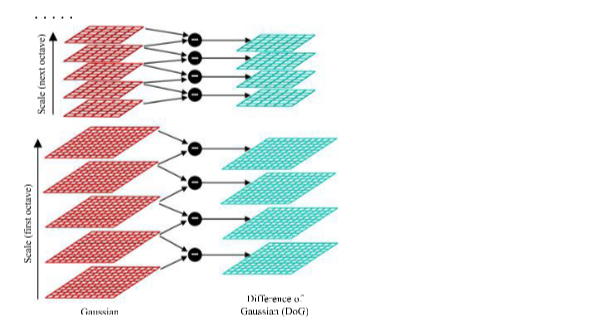
\includegraphics{Asset/image18.png}

}

\caption{Gambar 4.6. Formasi Laplacian Pyramid}

\end{figure}

\begin{itemize}
\tightlist
\item
  \textbf{Deteksi puncak dalam skala-ruang:} Pada tahap ini, titik-titik
  ekstrem lokal dideteksi dengan mempertimbangkan baik ruang maupun
  skala. Tujuannya adalah untuk mengidentifikasi lokasi dan skala yang
  dapat diberikan secara berulang dalam pandangan yang berbeda dari
  adegan atau objek yang sama. Pada kasus diskrit, hal ini ditentukan
  dengan membandingkan dengan 26 tetangga terdekat seperti yang
  ditunjukkan di Gambar 4.7.
\end{itemize}

\begin{figure}

{\centering 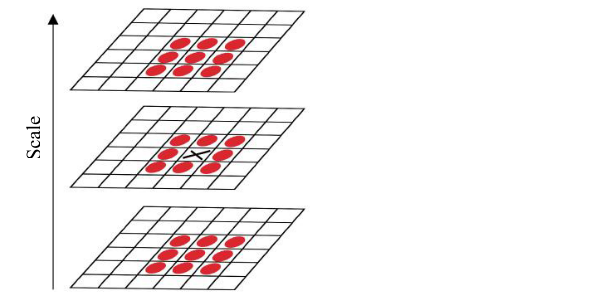
\includegraphics{Asset/image19.png}

}

\caption{Gambar 4.7. Scale-space peak detection}

\end{figure}

\begin{itemize}
\tightlist
\item
  \textbf{Lokalisasi titik kunci dan penolakan outlier:} Selanjutnya,
  skala yang memberikan ekstremum dalam perbedaan Gaussian ditetapkan
  sebagai skala untuk titik kunci. Namun, deteksi ekstremum dalam
  skala-ruang menghasilkan banyak calon titik kunci. Namun demikian,
  beberapa titik kunci tidak stabil. Oleh karena itu, langkah berikutnya
  dari algoritma ini adalah menolak beberapa titik kunci yang memiliki
  kontras rendah atau yang terlokalisasi buruk di sepanjang tepi. Titik
  kunci dengan kontras rendah sensitif terhadap noise.\\
  \textbf{Penghilangan titik kunci kontras rendah:} Titik kunci dengan
  kontras rendah dan terlokalisasi buruk dihilangkan dengan menggunakan
  interpolasi subpiksel/subskala menggunakan ekspansi Taylor, yang
  diberikan oleh:
\end{itemize}

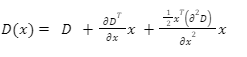
\includegraphics{Asset/image111.png}

Di mana, D dan turunannya dihitung di titik kunci calon dan x = (x, y, )
adalah offset dari titik ini. Lokasi puncak x diperkirakan dengan
mempertimbangkan turunan fungsi ini terhadap x dan mengatur nilainya
menjadi nol. Jika offset x lebih besar dari ambang batas yang telah
ditentukan dalam dimensi manapun, maka hal ini menunjukkan bahwa puncak
berada lebih dekat dengan titik kunci calon lainnya. Dalam hal ini,
titik kunci calon harus diubah dan interpolasi dilakukan di sekitar
titik tersebut. Jika tidak, offset ditambahkan ke titik kunci calon
tersebut. Hal ini dilakukan untuk mendapatkan perkiraan yang
diinterpolasi untuk lokasi puncak.\\
\textbf{Penghilangan respons tepi:} Titik-titik tepi sesuai dengan
kontras tinggi dalam satu arah dan rendah dalam arah lainnya. Fungsi DoG
memiliki respons kuat di sepanjang tepi gambar. Titik kunci yang
memiliki lokasi yang sangat tidak terdefinisi tetapi memiliki respons
tepi tinggi dihilangkan. Langkah ini meningkatkan stabilitas. Puncak
yang tidak terdefinisi dengan baik dalam fungsi DoG menunjukkan
kelengkungan tinggi di sepanjang tepi dan nilai rendah dalam arah tegak
lurus. Kelengkungan utama dapat dihitung dengan mengevaluasi matriks
Hessian. Perlu dicatat bahwa untuk puncak yang tidak terdefinisi dengan
baik dalam fungsi DoG, kelengkungan utama di sepanjang tepi jauh lebih
besar daripada kelengkungan utama sepanjangnya. Untuk menemukan
kelengkungan utama, kita perlu mencari solusi untuk eigenvalue dari
matriks Hessian orde kedua H sebagai berikut:\\
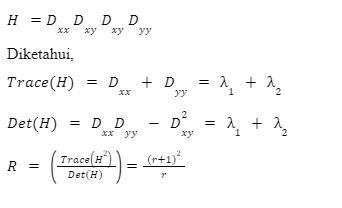
\includegraphics{Asset/image112.png}\\
Dalam persamaan di atas, rasio R hanya bergantung pada rasio eigenvalue
r = A1/A2, dan R minimum ketika eigenvalue sama satu sama lain. Jika
perbedaan absolut antara dua eigenvalue lebih tinggi, maka perbedaan
absolut antara dua kelengkungan utama D juga akan lebih tinggi. Ini
sesuai dengan nilai tinggi dari R. Oleh karena itu, eliminasi titik
kunci dilakukan jika:\\
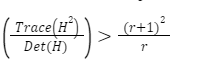
\includegraphics{Asset/image113.png}

\begin{itemize}
\item
  \textbf{Penugasan orientasi:} Pada langkah ini, setiap titik kunci
  diberikan satu atau lebih orientasi. Orientasi ditentukan berdasarkan
  arah gradien citra lokal. Deskriptor titik kunci dapat
  direpresentasikan relatif terhadap orientasi ini. Itulah sebabnya,
  mereka invariant terhadap rotasi citra. Untuk ini, magnitudo dan
  orientasi pada citra yang telah dihaluskan dengan Gaussian (pada skala
  yang sesuai dengan titik kunci) dihitung. Pertama, citra yang telah
  dihaluskan dengan Gaussian L(x,y,a) pada skala titik kunci a diambil
  agar semua perhitungan terkait dilakukan dalam cara yang invariant
  terhadap skala. Untuk sampel citra L(x,y) pada skala σ, magnitudo
  gradien m(x,y) dan orientasi θ(x,y) dihitung menggunakan perbedaan
  piksel sebagai berikut:\\
  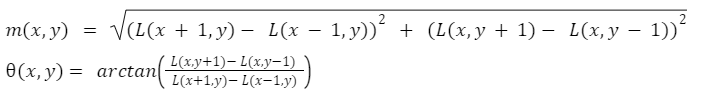
\includegraphics{Asset/image114.png}\\
  Perhitungan magnitudo dan arah untuk gradien harus dilakukan untuk
  setiap piksel tetangga di sekitar titik kunci dalam citra L yang telah
  dihaluskan dengan Gaussian. Selanjutnya, histogram orientasi dibentuk
  dari orientasi gradien titik sampel dalam sebuah wilayah di sekitar
  titik kunci. Histogram orientasi memiliki 36 bin yang mencakup rentang
  360 derajat orientasi. Setiap sampel yang ditambahkan ke histogram
  diberi bobot berdasarkan magnitudo gradiennya dan oleh jendela
  lingkaran berbobot Gaussian. Puncak-puncak dalam histogram ini sesuai
  dengan orientasi dominan dari patch citra. Pada skala dan lokasi yang
  sama, dapat ada beberapa titik kunci dengan orientasi yang berbeda.
  Jika terdapat penugasan beberapa orientasi, titik kunci tambahan harus
  dibuat. Titik kunci tambahan tersebut harus memiliki lokasi dan skala
  yang sama dengan titik kunci asli untuk setiap orientasi tambahan.
  Jadi, setiap titik kunci memiliki parameter (x, y, 2, θ).
\item
  \textbf{Deskriptor titik kunci:} Pada langkah-langkah sebelumnya,
  lokasi titik kunci pada skala tertentu telah ditemukan. Setelah itu,
  orientasi ditetapkan untuk titik kunci tersebut. Penugasan orientasi
  menjamin invariansi terhadap lokasi citra, skala, dan rotasi. Langkah
  selanjutnya adalah menghitung vektor deskriptor untuk masing-masing
  titik kunci. Tujuannya adalah membuat deskriptor menjadi sangat khas.
  Selain itu, deskriptor juga seharusnya sebagian invariant terhadap
  pencahayaan, sudut pandang 3D, dll. Langkah ini harus dilakukan pada
  citra yang paling mendekati skala titik kunci. Sebelum menghitung
  deskriptor, penting untuk memutar wilayah dengan nilai orientasi
  negatif (minus θ) yang terkait dengan titik kunci.\\
  Pertama, sejumlah histogram orientasi dibuat pada subwilayah
  (lingkungan) piksel 4x4, dan 8 bin dialokasikan untuk setiap
  subwilayah tersebut. Histogram ini berasal dari magnitudo dan nilai
  orientasi dari sampel dalam wilayah 16x16 di sekitar titik kunci.
  Jadi, setiap histogram berisi sampel dari subwilayah 4x4 dari wilayah
  lingkungan asli. Selanjutnya, magnitudo diberi bobot dengan fungsi
  Gaussian. Deskriptor kemudian menjadi vektor yang berisi semua nilai
  dari histogram-histogram ini. Karena terdapat 4x4 = 16 histogram,
  masing-masing dengan 8 bin, vektor tersebut akan memiliki 128 elemen.
  Jadi, dimensi deskriptor atau vektor fitur akan menjadi 128. Vektor
  ini kemudian dinormalisasi menjadi panjang satuan untuk mengurangi
  efek variasi pencahayaan. Gambar 4.8. dan 4.9. menunjukkan gradien
  gambar dan deskriptor titik kunci yang sesuai.
\end{itemize}

\begin{figure}

\begin{minipage}[t]{0.50\linewidth}

{\centering 

\raisebox{-\height}{

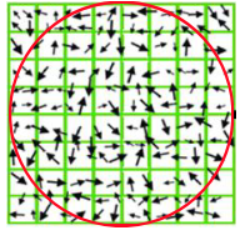
\includegraphics{Asset/image115.png}

}

\caption{Gambar 4.8. Cameraman Image}

}

\end{minipage}%
%
\begin{minipage}[t]{0.50\linewidth}

{\centering 

\raisebox{-\height}{

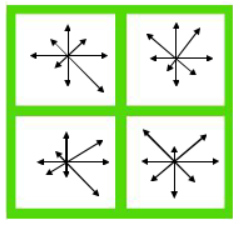
\includegraphics{Asset/image116.png}

}

\caption{Gambar 4.9. Cameraman Image dengan HOG}

}

\end{minipage}%

\end{figure}

Untuk aplikasi seperti pencarian gambar berbasis konten, fitur SIFT
dapat dihitung untuk sekumpulan gambar dalam basis data, dan
deskriptor-fiturnya disimpan dalam basis data tersebut. Begitu juga
untuk sebuah gambar query, fitur SIFT dapat dihitung. Untuk pencocokan,
deskriptor terdekat dalam basis data yang sesuai dengan deskriptor
gambar query dapat ditemukan dengan menggunakan metrik jarak yang
sesuai, dan gambar query tersebut dapat diambil kembali dari basis
data.\\
Proses pencarian dapat dilakukan dengan membandingkan deskriptor-fitur
gambar query dengan deskriptor-fitur gambar dalam basis data menggunakan
metrik jarak seperti jarak Euclidean atau jarak cosine. Metrik jarak
digunakan untuk mengukur sejauh mana kedua deskriptor-fitur tersebut
mirip satu sama lain. Jika terdapat kemiripan yang signifikan antara
deskriptor-fitur gambar query dengan deskriptor-fitur gambar dalam basis
data, gambar-gambar tersebut dapat dianggap sebagai pencocokan
potensial.\\
Setelah pencocokan dilakukan, gambar-gambar dalam basis data dapat
diurutkan berdasarkan tingkat kemiripan dengan gambar query.
Gambar-gambar yang memiliki deskriptor-fitur yang paling mirip dengan
gambar query akan muncul sebagai hasil teratas dalam hasil pencarian.
Dengan demikian, gambar-gambar dalam basis data yang memiliki fitur yang
mirip dengan gambar query dapat ditemukan dan dipulihkan dengan
menggunakan fitur-fitur SIFT. Penggunaan fitur-fitur SIFT dalam aplikasi
pencarian gambar berbasis konten memungkinkan pencarian yang lebih
akurat dan efisien dengan mengabaikan perubahan skala, rotasi, dan
pencahayaan dalam gambar.

\hypertarget{c.-bow-dan-bovw}{%
\section*{C. BoW dan BoVW}\label{c.-bow-dan-bovw}}
\addcontentsline{toc}{section}{C. BoW dan BoVW}

\markright{C. BoW dan BoVW}

Bag of Word (BOW) pada awalnya tidak digunakan untuk visi komputer namun
digunakan dalam bidang Text-Processin. Terkadang dalam konteks visi
komputer Bag of Word disebut juga Bag of Visual Word. Namun Kita tetap
akan menggunakan istilah BOW karena ini adalah istilah yang digunakan
pada OpenCV.

BoW adalah teknik yang digunakan untuk memberikan bobot atau hitungan
untuk setiap kata dalam rangkaian dokumen; kita kemudian
merepresentasikan dokumen-dokumen ini dengan vektor-vektor dari jumlah
ini. Mari kita lihat pada sebuah contoh, sebagai berikut:\\
\textbf{Dokumen 1:} Saya suka Python dan Saya suka Java \textbf{Dokumen
2:} Saya suka Python dan C\# \textbf{Dokumen 3:} Saya tidak suka
pemrograman

Dari ketiga dokumen diatas dapat dibuat kamus atau kosakata, dengan
nilai nilai sebagai berikut:

\begin{Shaded}
\begin{Highlighting}[]
\NormalTok{\{  }
\NormalTok{    Saya : 4   }
\NormalTok{    suka : 4  }
\NormalTok{    Python : 2  }
\NormalTok{    dan : 2  }
\NormalTok{    Java : 1  }
\NormalTok{    C\# : 1  }
\NormalTok{    tidak : 1  }
\NormalTok{    pemrograman : 1  }
\NormalTok{\} }
\end{Highlighting}
\end{Shaded}

Kita memiliki 8 entri atau fitur yang nantinya akan direpresentasikan
untuk dokumen 1,2, dan 3. Setiap vektor berisi nilai yang mewakili
jumlah semua kata dalam kamus secara berurutan, untuk dokumen tertentu.
Representasi vektor dari tiga kalimat sebelumnya adalah sebagai berikut:

\begin{figure}

{\centering 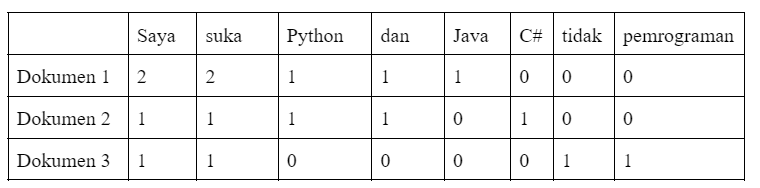
\includegraphics{Asset/image117.png}

}

\caption{Tabel 4.1 Representasi BoW}

\end{figure}

Vektor-vektor ini dapat di konseptualisasikan sebagai representasi
histogram dari sebuah dokumen atau sebagai vektor deskriptor yang dapat
digunakan untuk pengklasifikasian.

Konsep BOVW(Bag of Visual Word) diadaptasi dari BOW(Bag of Word) serta
Information Retrieval yang ada pada NLP(Natural language Processing).
BOW(Bag of Wors) bekerja dengan memakai frekuensi tiap kata-kata supaya
mengetahui keywoard dari dokumen dengan menghitung berapa jumlah setiap
katta yang muncul di dokumen (Davida, 2018).\\
Yang membedakan BOVW dengan BOW yaitu pada BOW yang digunakan adalah
kata-kata, sedangkan BOVW menggunakan fitur-fitur gambar atau bisa
dikatakan pola unik pada gambar yang berperan sebagai ``kata-kata'' yang
ada di BOW. Setelah menghitung frekuensi, maka dari perhitungan
frekuensi tersebut setiap fitur-fitur gambar dibuat histogram. Fitur itu
sendiri tersusun dari deskriptor dan keypoints (Davida, 2018).\\
Sesuai dengan namanya, keypoints merupakan titik-titik yang menunjukan
bagian-bagian gambar yang ``menonjol''. Sedangkan deskriptor adalah
gambaran dari keypoint. Dengan begitu, walaupun gambar dikecilkan,
diperluas, diputar, letak titik-titik keypoint-nya akan tetap sama.
Histogram frekuensi yang terbentuk dapat digunakan untuk memprediksi
kategori citra serta menemukan citra lainnya yang mirip atau serupa
(Davida, 2018).

\begin{figure}

{\centering 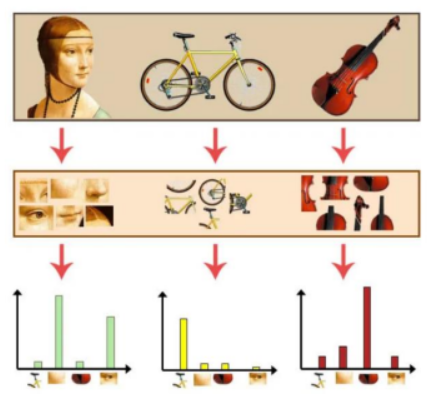
\includegraphics{Asset/image118.png}

}

\caption{Gambar 4.10. Ilustrasi BoVW}

\end{figure}

\hypertarget{konsep-dasar-machine-learning-dan-deep-learning-dalam-klasifikasi-objek}{%
\chapter*{5 Konsep Dasar Machine Learning dan Deep Learning dalam
Klasifikasi
Objek}\label{konsep-dasar-machine-learning-dan-deep-learning-dalam-klasifikasi-objek}}
\addcontentsline{toc}{chapter}{5 Konsep Dasar Machine Learning dan Deep
Learning dalam Klasifikasi Objek}

\markboth{5 Konsep Dasar Machine Learning dan Deep Learning dalam
Klasifikasi Objek}{5 Konsep Dasar Machine Learning dan Deep Learning
dalam Klasifikasi Objek}

\hypertarget{pengenalan-klasifikasi-objek}{%
\section*{Pengenalan Klasifikasi
Objek}\label{pengenalan-klasifikasi-objek}}
\addcontentsline{toc}{section}{Pengenalan Klasifikasi Objek}

\markright{Pengenalan Klasifikasi Objek}

Klasifikasi gambar mengacu pada proses pengelompokan atau pelabelan
gambar ke dalam kelas atau kategori yang berbeda berdasarkan konten
visualnya. Ini adalah tugas mendasar dalam visi komputer dan
pembelajaran mesin. Tujuan dari klasifikasi gambar adalah untuk
mengembangkan algoritma atau model yang secara otomatis dapat mengenali
dan memberikan label atau kategori yang tepat pada gambar yang
diberikan.\\
Algoritma klasifikasi gambar menggunakan berbagai teknik dan pendekatan
untuk menganalisis fitur visual dari sebuah gambar dan membuat prediksi.
Teknik-teknik ini dapat berkisar dari metode tradisional yang didasarkan
pada fitur buatan tangan hingga model pembelajaran mendalam yang lebih
canggih.\\
Berikut adalah beberapa poin penting tentang klasifikasi gambar:

\begin{itemize}
\tightlist
\item
  Ekstraksi fitur: Algoritma klasifikasi gambar mengekstrak fitur yang
  relevan dari gambar untuk merepresentasikan konten visualnya.
  Fitur-fitur ini dapat mencakup warna, tekstur, bentuk, dan informasi
  spasial. Contoh algoritma yang dapat digunakan untuk ekstraksi fitur
  adalah HOG dan SIFT.\\
\item
  Fase pelatihan: Pada tahap pelatihan, sebuah model dilatih menggunakan
  kumpulan data berlabel, di mana setiap gambar dikaitkan dengan kelas
  atau kategori yang diketahui. Model belajar mengenali pola dan
  hubungan antara fitur yang diekstrak dan label yang sesuai.\\
\item
  Fase klasifikasi: Pada fase klasifikasi, model yang telah dilatih
  digunakan untuk memprediksi kelas atau kategori gambar baru yang belum
  terlihat. Model ini menganalisis fitur visual dari gambar input dan
  membandingkannya dengan pola yang telah dipelajari untuk membuat
  prediksi.\\
\item
  Supervised Learning: Klasifikasi gambar biasanya dilakukan dengan
  menggunakan algoritma pembelajaran yang diawasi, di mana set data
  pelatihan diberi label dengan anotasi kebenaran dasar. Model belajar
  dari contoh-contoh berlabel ini untuk menggeneralisasi dan membuat
  prediksi pada data yang tidak terlihat.
\item
  Deep Learning: Model pembelajaran mendalam, seperti convolutional
  neural network (CNN), telah merevolusi klasifikasi gambar. CNN
  dirancang untuk secara otomatis mempelajari representasi hirarkis
  gambar, menangkap fitur tingkat rendah dan tingkat tinggi. Mereka
  telah mencapai kinerja canggih pada berbagai tugas klasifikasi gambar.
\item
  Aplikasi: Klasifikasi gambar memiliki banyak aplikasi di berbagai
  bidang, termasuk pengenalan objek, deteksi wajah, pencitraan medis,
  kendaraan otonom, dan pengambilan gambar berbasis konten.
\end{itemize}

\hypertarget{k-nearest-neighbors-knn}{%
\section*{K-Nearest Neighbors (KNN)}\label{k-nearest-neighbors-knn}}
\addcontentsline{toc}{section}{K-Nearest Neighbors (KNN)}

\markright{K-Nearest Neighbors (KNN)}

\url{https://youtu.be/HNoZHBDa_dA}

K-Nearest Neighbors adalah salah satu algoritma Supervised Learning yang
dapat digunakan untuk melakukan klasifikasi citra. Algoritma ini
termasuk dalam jenis algoritma pembelajaran berbasis instans atau
instance-based learning. KNN bekerja berdasarkan objek yang memiliki
atribut yang mirip cenderung memiliki label atau nilai target yang mirip
pula.

\textbf{Konsep Dasar:}

\begin{itemize}
\tightlist
\item
  KNN beroperasi dengan menggunakan data latih yang berlabel dan
  mengklasifikasikan atau memperkirakan label dari data yang tidak
  diketahui.\\
\item
  KNN menggunakan jarak (euclidean, manhattan, dll.) untuk mengukur
  kedekatan antara data.\\
\item
  Konsep dasar KNN adalah ``yang mirip, dikelompokkan bersama.''\\
\item
  KNN tidak melakukan proses pembelajaran pada tahap pelatihan, tetapi
  menyimpan semua data latih sebagai basis pengetahuan.
\end{itemize}

\begin{figure}

{\centering 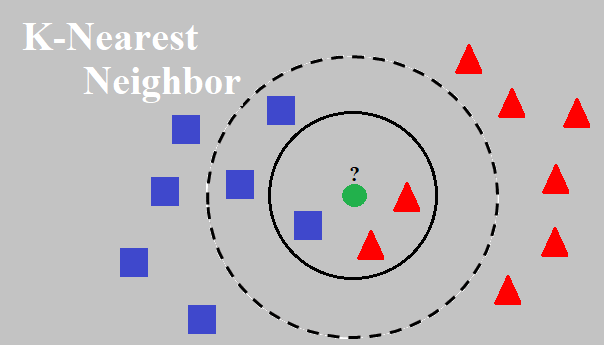
\includegraphics{Asset/knnilustration.png}

}

\caption{Gambar 5.1 Ilustrasi KNN}

\end{figure}

\textbf{Langkah-Langkah KNN:}

\begin{itemize}
\tightlist
\item
  Menentukan jumlah tetangga terdekat (K) yang akan digunakan dalam
  pengklasifikasian.\\
\item
  Menghitung jarak antara data yang tidak diketahui dengan setiap contoh
  data latih menggunakan metrik jarak yang sesuai.\\
\item
  Mengidentifikasi K contoh data latih terdekat berdasarkan jarak yang
  dihitung sebelumnya.\\
\item
  Menggunakan mayoritas voting (untuk klasifikasi) atau rata-rata (untuk
  regresi) dari label tetangga terdekat untuk memprediksi label atau
  nilai target dari data yang tidak diketahui.\\
\item
  Mengeluarkan prediksi sebagai hasil.
\end{itemize}

\textbf{Pemilihan Nilai K:}

\begin{itemize}
\tightlist
\item
  Pemilihan nilai K yang tepat sangat penting dalam KNN. Nilai K yang
  salah dapat mengakibatkan overfitting atau underfitting.\\
\item
  Jika K terlalu kecil (misalnya K = 1), model akan cenderung terlalu
  responsif terhadap data latih yang spesifik dan lebih rentan terhadap
  noise.\\
\item
  Jika K terlalu besar, informasi dari tetangga yang sebenarnya relevan
  dapat terlupakan, yang dapat menyebabkan kesalahan klasifikasi.
\end{itemize}

\textbf{Perhitungan Jarak}\\
Perhitungan jarak dalam KNN adalah langkah penting dalam menentukan
tetangga terdekat untuk titik data yang diberikan. Metrik jarak mengukur
kemiripan atau ketidakmiripan antara dua titik data dan digunakan untuk
menemukan K tetangga terdekat. Ada beberapa perhitungan jarak yang bisa
digunakan dalam algoritma KNN:

\begin{enumerate}
\def\labelenumi{\alph{enumi})}
\item
  Jarak Euclidean: Ini adalah jarak garis lurus antara dua titik dalam
  ruang Euclidean. Metrik ini menghitung akar kuadrat dari jumlah
  perbedaan kuadrat antara fitur-fitur yang sesuai dari dua titik data.

  Bila dalam kasus lain terdapat lebih dari 2 variabel, kita bisa
  menggunakan rumus euclidean distance seperti gambar 5.2. Mirip dengan
  rumus pythagoras, hanya saja Euclidean Distance memiliki dimensi lebih
  dari 2.
\end{enumerate}

\begin{figure}

{\centering 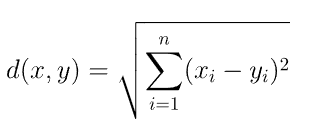
\includegraphics{Asset/euclideanrumus.png}

}

\caption{Gambar 5.2 Rumus Euclidean Distance}

\end{figure}

\begin{enumerate}
\def\labelenumi{\alph{enumi})}
\setcounter{enumi}{1}
\tightlist
\item
  Jarak Manhattan: Juga dikenal sebagai jarak blok kota atau jarak L1,
  jarak ini menghitung jumlah perbedaan absolut antara fitur-fitur yang
  sesuai dari dua titik data. Jarak ini mengukur jarak dengan bergerak
  hanya dalam arah horizontal atau vertikal. Perhitungan Manhattan
  Distance dapat dituliskan seperti pada Gambar 5.3.
\end{enumerate}

\begin{figure}

{\centering 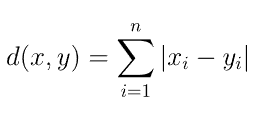
\includegraphics{Asset/manhattandistance.png}

}

\caption{Gambar 5.3 Rumus Manhattan Distance}

\end{figure}

\begin{enumerate}
\def\labelenumi{\alph{enumi})}
\setcounter{enumi}{2}
\tightlist
\item
  Jarak Minkowski: Ini adalah generalisasi dari jarak Euclidean dan
  Manhattan. Jarak ini menghitung akar ke-n dari jumlah nilai absolut
  yang dipangkatkan dengan pangkat n dari perbedaan antara fitur-fitur
  yang sesuai dari dua titik data. Perhitungan Minkowski Distance dapat
  dituliskan seperti pada gambar 5.4.
\end{enumerate}

\begin{figure}

{\centering 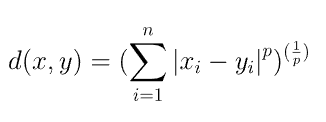
\includegraphics{Asset/minkowskidistance.png}

}

\caption{Gambar 5.4 Rumus Minkowski Distance}

\end{figure}

\begin{figure}

{\centering 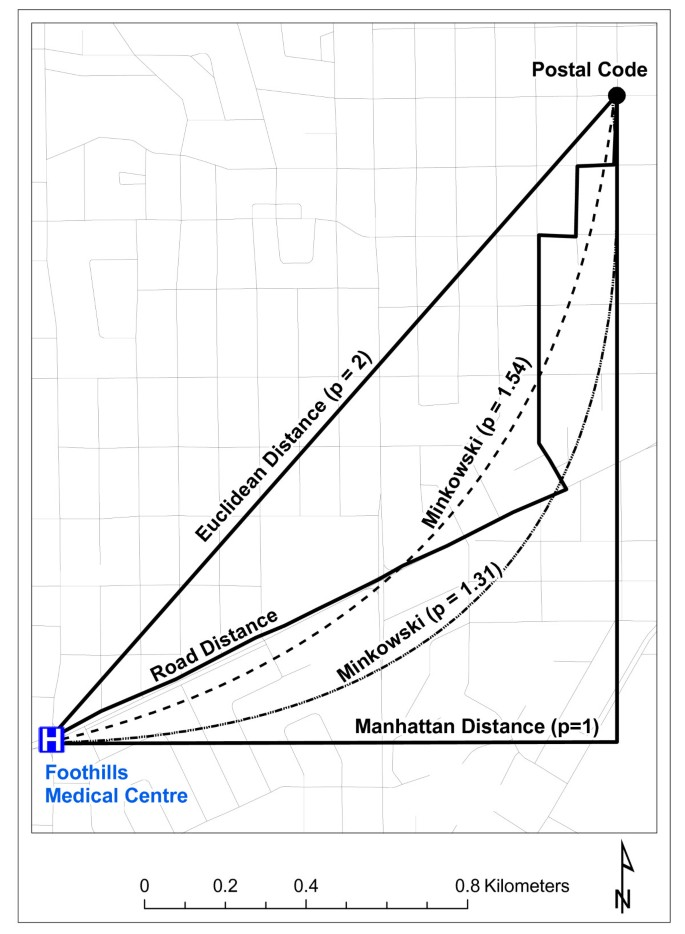
\includegraphics{Asset/perbandingan_jarak.jpg}

}

\caption{Gambar 5.5 Perbandingan Perhitungan Jarak dalam KNN}

\end{figure}

\textbf{Kelebihan K-Nearest Neighbors:}

\begin{itemize}
\tightlist
\item
  Sederhana dan mudah diimplementasikan.\\
\item
  KNN dapat digunakan untuk masalah klasifikasi dan regresi.\\
\item
  Algoritma non-parametrik, sehingga tidak bergantung pada asumsi
  tertentu tentang distribusi data.\\
\item
  Mampu menangani data yang kompleks, termasuk data yang tidak linear.
\end{itemize}

\textbf{Kekurangan K-Nearest Neighbors:}

\begin{itemize}
\tightlist
\item
  KNN membutuhkan penyimpanan data latih yang lengkap untuk membuat
  prediksi, yang dapat memakan banyak memori.\\
\item
  KNN memiliki kompleksitas komputasi yang tinggi saat menghitung jarak
  ke semua contoh data latih.\\
\item
  Rentan terhadap adanya atribut yang dominan karena menggunakan jarak
  euclidean, sehingga atribut dengan skala besar dapat mendominasi
  atribut dengan skala kecil.
\end{itemize}

\hypertarget{convolutional-neural-network-cnn}{%
\section*{Convolutional Neural Network
(CNN)}\label{convolutional-neural-network-cnn}}
\addcontentsline{toc}{section}{Convolutional Neural Network (CNN)}

\markright{Convolutional Neural Network (CNN)}

Convolutional Neural Network (CNN) adalah algoritma Deep Learning yang
dirancang khusus untuk bekerja dengan gambar dan video. Algoritma ini
mengambil gambar sebagai input, mengekstrak dan mempelajari fitur-fitur
dari gambar tersebut, dan mengklasifikasikannya berdasarkan fitur-fitur
yang telah dipelajari.

Algoritma ini terinspirasi dari cara kerja bagian otak manusia, yaitu
Korteks Visual. Korteks visual adalah bagian dari otak manusia yang
bertanggung jawab dalam memproses informasi visual dari dunia luar.
Bagian ini terdiri dari beberapa lapisan, di mana setiap lapisan
memiliki fungsinya sendiri. Setiap lapisan mengekstrak informasi
tertentu dari gambar atau visual, dan pada akhirnya semua informasi yang
diterima dari setiap lapisan digabungkan untuk menginterpretasikan atau
mengklasifikasikan gambar atau visual tersebut.

Demikian pula, CNN memiliki berbagai filter, di mana setiap filter
mengekstrak informasi tertentu dari gambar seperti tepi, berbagai jenis
bentuk (vertikal, horizontal, bulat), dan sebagainya. Semua informasi
ini kemudian digabungkan untuk mengidentifikasi gambar tersebut.

\begin{figure}

{\centering \includegraphics{Asset/cnnillustration.jpeg}

}

\caption{Gambar 5.6 Ilustrasi CNN}

\end{figure}

\textbf{Konsep Dasar CNN:}

\begin{itemize}
\tightlist
\item
  CNN terdiri dari beberapa lapisan yang berbeda, termasuk lapisan
  konvolusi, lapisan pooling, dan lapisan fully connected.\\
\item
  Arsitektur CNN didasarkan pada prinsip penggunaan ulang parameter
  dengan menggunakan filter konvolusi yang sama pada seluruh data
  input.\\
\item
  Konvolusi adalah operasi yang melibatkan pergeseran filter konvolusi
  (kernel) pada data input untuk menghasilkan peta fitur atau feature
  map.\\
\item
  Pooling digunakan untuk mengurangi dimensi spasial dari feature map
  yang dihasilkan oleh lapisan konvolusi.\\
\item
  Fully connected layer menghubungkan setiap neuron di lapisan
  sebelumnya ke setiap neuron di lapisan berikutnya, mirip dengan
  jaringan saraf biasa.
\end{itemize}

Untuk gambaran lebih detailnya dapat kita lihat di
\href{http://playground.tensorflow.org/}{Tensorflow Playground}

\textbf{Langkah-langkah Algoritma CNN}

\begin{enumerate}
\def\labelenumi{\alph{enumi})}
\item
  Convolutional Layer

  Langkah pertama adalah lapisan konvolusi, di mana filter konvolusi
  bergerak melalui data input dan melakukan operasi konvolusi. Filter
  konvolusi berukuran kecil dan dapat dipelajari oleh algoritma. Setiap
  filter menghasilkan peta fitur dengan mengekstraksi pola spesifik dari
  data input. Selama konvolusi, filter dikalikan dengan bagian dari data
  input yang sedang diperiksa dan hasilnya dijumlahkan untuk membentuk
  elemen peta fitur.
\end{enumerate}

\begin{figure}

{\centering \includegraphics{Asset/convolutional.jpeg}

}

\caption{Gambar 5.7 Ilustrasi Convolutional}

\end{figure}

Dengan menggeser convolve filter disetiap kemungkinan posisi filter pada
gambar, dihasilkan sebuah activation map.

\includegraphics{Asset/conv2.gif}

Proses ini diulang dengan beberapa filter berbeda, hingga menghasilkan
gambar baru yang merupakan kumpulan dari activation maps.

\begin{enumerate}
\def\labelenumi{\alph{enumi})}
\setcounter{enumi}{1}
\item
  Pooling Layer

  Setelah lapisan konvolusi, lapisan pooling digunakan untuk mengurangi
  resolusi spasial dari peta fitur.\\
  Tujuan pooling adalah untuk mengurangi dimensi dan kompleksitas
  komputasi sambil mempertahankan fitur penting.\\
  Metode pooling yang paling umum digunakan adalah max pooling. Namun
  terdapat metode pooling lain yang dapat digunakan seperti Average
  Pooling dan L2 Norm Pooling.
\end{enumerate}

\begin{figure}

{\centering \includegraphics{Asset/pooling.png}

}

\caption{Gambar 5.8 Perbedaan Max Pooling dan Average Pooling}

\end{figure}

\begin{enumerate}
\def\labelenumi{\alph{enumi})}
\setcounter{enumi}{2}
\item
  Flattening

  Flattening merupakan proses mengubah representasi matriks
  multidimensional menjadi vektor satu dimensi. Proses flattening
  dilakukan dengan mengambil semua elemen dalam matriks multidimensional
  dan menyusunnya menjdi satu baris.
\end{enumerate}

\begin{figure}

{\centering \includegraphics{Asset/flatening.png}

}

\caption{Gambar 5.9 Proses Flattening}

\end{figure}

\begin{enumerate}
\def\labelenumi{\alph{enumi})}
\setcounter{enumi}{3}
\item
  Fully Connected Layer

  Setelah diperatakan menjadi vektor dan disambungkan ke lapisan fully
  connected.\\
  Lapisan ini bertindak sebagai klasifikasi akhir atau lapisan regresi,
  di mana prediksi akhir dilakukan berdasarkan fitur-fitur yang telah
  dipelajari.
\end{enumerate}

\begin{figure}

{\centering \includegraphics{Asset/fullyconnectedLayer.jpg}

}

\caption{Gambar 5.10 Fully Connected Layer}

\end{figure}

\begin{enumerate}
\def\labelenumi{\alph{enumi})}
\setcounter{enumi}{4}
\item
  Pelatihan

  Dalam fase pelatihan, CNN memperbarui bobot dan bias filter konvolusi
  serta parameter lapisan fully connected dengan meminimalkan fungsi
  loss antara prediksi dan label yang benar.\\
  Optimizer seperti Stochastic Gradient Descent (SGD) atau Adam
  digunakan untuk mengatur laju pembelajaran dan memperbarui parameter
  secara iteratif.
\end{enumerate}

\hypertarget{transfer-learning}{%
\section*{Transfer Learning}\label{transfer-learning}}
\addcontentsline{toc}{section}{Transfer Learning}

\markright{Transfer Learning}

\hypertarget{definisi-dan-konsep-dasar-transfer-learning}{%
\subsection*{Definisi dan Konsep Dasar Transfer
Learning}\label{definisi-dan-konsep-dasar-transfer-learning}}
\addcontentsline{toc}{subsection}{Definisi dan Konsep Dasar Transfer
Learning}

Transfer learning merupakan proses atau pendekatan dalam pembelajaran
mesin dimana pengetahuan yang didapatkan dari pelatihan model pada suatu
tugas, dapat digunakan pada tugas lain yang memiliki kemiripan dengan
masalah yang sedang dipecahkan. Pada konteks Convolutional Neural
Networks (CNN), transfer learning mengacu pada penggunaan model yang
sebelumnya sudah dilatih pada tugas pemrosesan citra untuk diadaptasi ke
tugas yang baru. Dalam pengembangan model Convolutional Neural Networks
(CNN), transfer learning cukup penting, dikarenakan transfer learning
dapat menghemat waktu dan sumber daya, hal ini dikarenakan untuk melatih
model CNN dari awal membutuhkan waktu yang cukup lama serta komputasi
yang besar. Sedangkan jika menggunakan transfer learning kita dapat
menggunakan model yang sudah ada. Yang kedua, performa akan menjadi
lebih baik dikarenakan model telah mempelajari fitur-fitur umum dari
data citra yang dapat diimplementasikan pada tugas yang baru. Jika kita
memiliki dataset yang terbatas, transfer learning dapat membantu dalam
pemanfaatan pengetahuan yang sudah ada dari dataset yang lebih banyak
pada tugas sebelumnya. Transfer learning juga dapat mengatasi masalah
overfitting yang sering terjadi pada model yang dilatih menggunakan
dataset yang kecil. Semakin mirip tugas pertama dengan tugas yang baru
maka akan semakin lebih baik. Dalam Deep Learning, pelatihan model pada
tugas pertama dinamakan pre-training, sedangkan penerapan model yang
sudah dilatih pada tugas pertama ke training model tugas baru dinamakan
fine-tuning.

\begin{figure}

{\centering \includegraphics{Asset/transferlearning.png}

}

\caption{Gambar 5.11 Illustrasi Transfer Learning pada CNN}

\end{figure}

\hypertarget{langkah-langkah-transfer-learning-pada-cnn}{%
\subsection*{Langkah-langkah Transfer Learning pada
CNN}\label{langkah-langkah-transfer-learning-pada-cnn}}
\addcontentsline{toc}{subsection}{Langkah-langkah Transfer Learning pada
CNN}

Setelah memahami definisi dan konsep dasar dari transfer learning,
selanjutnya adalah memahami langkah-langkah transfer learning khususnya
pada Convolutional Neural Networks (CNN). Berikut merupakan
langkah-langkah yang diperlukan :

\begin{itemize}
\item
  Seleksi model dasar\\
  Pertama-tama dilakukan pemilihan arsitektur dasar model CNN. Terdapat
  beberapa arsitektur yang terbukti efektif dalam pemrosesan citra yaitu
  seperti VGG, ResNet, Inception dan MobileNet. Arsitektur-arsitektur
  tersebut memiliki berbagai lapisan konvolusi, pooling dan fully
  connected yang akan membantu dalam ekstraksi fitur.
\item
  Feature Extraction Setelah memilih arsitektur dasar model, selanjutnya
  model dasar tersebut digunakan sebagai ekstraktor fitur. Pada
  lapisan-lapisan konvolusi awal telah mempelajari fitur-fitur umum dari
  dataset yang besar dan beragam. Fitur-fitur tersebut merupakan hasil
  ekstraksi pola yaitu tepi, tekstur, dan bentuk dari gambar.
\item
  Fine-tuning\\
  Lapisan-lapisan akhir kebanyakan berfungsi sebagai klasifikasi atau
  regresi, dengan dilakukan fine-tuning model dapat menyesuaikan
  representasi-fitur yang lebih spesifik untuk tugas yang baru. Pada
  fine-tuning, model dapat dilatih ulang menggunakan dataset khusus
  disesuaikan dengan tugas yang ingin diselesaikan.
\item
  Freezing Layers\\
  Dalam transfer learning, freezing layer tidak selalu wajib diterapkan
  dikarenakan hal tersebut bergantung pada karakteristik tugas dan
  sumberdaya yang tersedia. Freezing layer merupakan pengamanan nilai
  bobot pada beberapa lapisan awal model dasar(lapisan konvolusi awal)
  sehingga tidak mengalami perubahan pada pelatihan ulang. Hal ini
  mengakibatkan fitur-fitur umum tetap tidak berubah, sedangkan lapisan
  akhir yang lebih spesifik disesuaikan.
\item
  Domain Similarity\\
  Transfer learning yang paling efektif yaitu ketika domain data
  pelatihan awal(domain asal) memiliki kemiripan atau kesamaan dengan
  domain data tugas baru(domain target).Domain adalah kumpulan data yang
  berasal dari sumber tertentu. Sedangkan domain similarity sendiri
  merupakan sejauh mana dua domain data memiliki kemiripan atau kesamaan
  dalam hal fitur, distribusi, karakteristik, atau pola. Jika kedua
  domain kemiripannya tinggi, maka akan berpotensi besar untuk
  diadaptasi karena relevan.
\item
  Data Augmentation\\
  Augmentasi data merupakan teknik untuk memperkaya dataset pelatihan
  yaitu dengan berbagai variasi citra seperti rotasi, pergeseran, dan
  perubahan ukuran citra. Dengan begitu peningkatan generalisasi model
  akan meningkat.
\item
  Pengaturan Parameter\\
  Selama transfer learning, perlu dilakukan penyesuaian parameter
  seperti learning rate dan batch size supaya sesuai dengan
  karakteristik dataset dan tugas baru.
\item
  Evaluasi dan Fine-tuning\\
  Setelah tahap fine-tuning, model dievaluasi pada dataset validasi dan,
  jika diperlukan, dapat dilakukan fine-tuning lebih lanjut guna
  memperbaiki performa.
\end{itemize}

\hypertarget{mobilenet}{%
\subsection*{MobileNet}\label{mobilenet}}
\addcontentsline{toc}{subsection}{MobileNet}

Pada tahap seleksi model dasar pada fine tuning, terdapat beberapa
arsitektur yang dapat dipilih seperti VGG, ResNet, Inception dan
MobileNet. Pada kali ini akan dibahas mengenai MobileNet. Arsitektur
MobileNet adalah salah satu arsitektur pada Convolutional Neural
Networks (CNN) yang berguna dalam mengatasi kebutuhan computing resource
yang berlebih. Arsitektur ini dibuat oleh para peneliti Google yang mana
dapat digunakan untuk ponsel. Konvolusi pada MobileNet terbagi menjadi
dua yaitu depthwise convolution dan pointwise convolution seperti pada
gambar 5.12 dan gambar 5.13. Pada gambar 5.14 merupakan arsitektur dari
MobileNet.

\begin{figure}

{\centering \includegraphics{Asset/mobilenet1.png}

}

\caption{Gambar 5.12 Konvolusi Standar (a) dibagi menjadi dua lapisan:
depthwise convolution (b) dan pointwise convolution (c) untuk membuat
sebuah filter secara mendalam (depthwise)}

\end{figure}

\begin{figure}

{\centering \includegraphics{Asset/mobilenet2.png}

}

\caption{Gambar 5.13 Kiri: lapisan konvolusi standard dengan batchnorm
dan ReLU. Kanan: Depthwise convolution dan Pointwise convolution dengan
batchnorm dan ReLU.}

\end{figure}

\begin{figure}

{\centering \includegraphics{Asset/mobilenet3.png}

}

\caption{Gambar 5.14 Arsitektur MobileNet}

\end{figure}

MobileNet memiliki beberapa versi, per September 2021 versi MobileNet
terdapat 3 versi yaitu MobileNetV1, MobileNetV2, dan MobileNetV3. Untuk
MobileNetV2 dirilis pada April 2017 lalu. MobileNetV2 masih menggunakan
depthwise dan pointwise convolution. Dari versi MobileNetV1 ke
MobileNetV2 dilakukan peningkatan yaitu dengan menambahkan dua fitur
baru yaitu linear bottleneck dan shortcut connections antar bottlenecks.
Struktur arsitektur dari MobileNetV2 dapat dilihat pada gambar 4 di
bawah.

\begin{figure}

{\centering \includegraphics{Asset/mobilenetv2.png}

}

\caption{Gambar 5.15 Arsitektur MobilenetV2. Kotak biru menunjukkan blok
pembentukkan konvolusi linear bottleneck}

\end{figure}

Diantara model terdapat input dan output pada bagian bottleneck,
sedangkan pada layer bagian dalam dilakukan enkapsulasi kemampuan model
guna mengubah input dari konsep tingkat yang lebih rendah (i.e.~piksel)
ke deskriptor tingkat yang lebih tinggi (i.e.~kategori gambar). Shortcut
antar bottlenecks memungkinkan training atau pelatihan yang lebih cepat
dan akurasi yang lebih baik, hal ini seperti koneksi residual pada CNN
tradisional.

\begin{figure}

{\centering \includegraphics{Asset/mobilenetars.png}

}

\caption{Gambar 5.16 Arsitektur MobileNet V2}

\end{figure}

\hypertarget{metode-evaluasi-dalam-computer-vision}{%
\chapter*{6 Metode Evaluasi dalam Computer
Vision}\label{metode-evaluasi-dalam-computer-vision}}
\addcontentsline{toc}{chapter}{6 Metode Evaluasi dalam Computer Vision}

\markboth{6 Metode Evaluasi dalam Computer Vision}{6 Metode Evaluasi
dalam Computer Vision}

\hypertarget{confusion-matrix}{%
\section*{Confusion Matrix}\label{confusion-matrix}}
\addcontentsline{toc}{section}{Confusion Matrix}

\markright{Confusion Matrix}

Confusion Matrix digunakan untuk mengukur performa model klasifikasi
dengan membandingkan hasil klasifikasi dari model dengan nilai
sebenarnya pada dataset yang digunakan. Confusion matrix terdiri dari
empat jenis nilai, yaitu True Positive (TP), True Negative (TN), False
Positive (FP), dan False Negative (FN). Dengan menggunakan confusion
matrix, dapat diperoleh gambaran yang jelas tentang seberapa baik
kinerja model klasifikasi yang digunakan dalam memprediksi data pada
dataset yang diberikan.\\
Terdapat beberapa metrik yang dapat dihitung berdasarkan nilai-nilai
pada confusion matrix, antara lain:

\begin{enumerate}
\def\labelenumi{\alph{enumi}.}
\tightlist
\item
  Accuracy: mengukur seberapa akurat model dalam melakukan klasifikasi
  pada dataset. Rumusnya adalah (TP + TN) / (TP + TN + FP + FN).\\
\item
  Precision: mengukur seberapa akurat model dalam memprediksi data
  positif. Rumusnya adalah TP / (TP + FP).\\
\item
  Recall: mengukur seberapa banyak data positif yang dapat terdeteksi
  oleh model. Rumusnya adalah TP / (TP + FN).\\
\item
  F1-Score: merupakan harmonic mean dari precision dan recall. Rumusnya
  adalah 2 * (Precision * Recall) / (Precision + Recall).
\end{enumerate}

Berdasarkan nilai-nilai pada confusion matrix, dapat diketahui apakah
model klasifikasi yang dibangun sudah bekerja dengan baik atau belum.
Beberapa hal yang dapat diinterpretasikan dari confusion matrix antara
lain:

\begin{itemize}
\tightlist
\item
  True Positive (TP): jumlah data positif yang berhasil diprediksi
  dengan benar oleh model.\\
\item
  True Negative (TN): jumlah data negatif yang berhasil diprediksi
  dengan benar oleh model.\\
\item
  False Positive (FP): jumlah data negatif yang salah diprediksi sebagai
  positif oleh model.\\
\item
  False Negative (FN): jumlah data positif yang salah diprediksi sebagai
  negatif oleh model.
\end{itemize}

\begin{figure}

{\centering \includegraphics{Asset/confusion_matrix.png}

}

\caption{Gambar 5.8 Confussion Matrix}

\end{figure}

\textbf{Confusion Matrix Multiclass}

\href{https://www.analyticsvidhya.com/blog/2021/06/confusion-matrix-for-multi-class-classification/}{Confusion
Matrix Multiclass}.

Confusion Matrix juga dapat digunakan untuk menganalisis performa model
pada data dengan multi kelas atau multi class.

Dalam konteks data multi class, confusion matrix akan memiliki dimensi
yang sesuai dengan jumlah kelas yang ada. Setiap sel dalam matriks
mewakili jumlah sampel yang diklasifikasikan dengan benar atau salah ke
suatu kelas tertentu. Baris dalam matriks mewakili kelas sebenarnya,
sedangkan kolom mewakili kelas yang diprediksi oleh model.

Dengan menggunakan confusion matrix pada data multi class, kita dapat
menghitung metrik evaluasi seperti akurasi, presisi, recall, dan
F1-score untuk setiap kelas secara individu. Akurasi mengukur sejauh
mana model secara keseluruhan mengklasifikasikan dengan benar, sedangkan
presisi, recall, dan F1-score memberikan wawasan lebih rinci tentang
kinerja model untuk setiap kelas secara terpisah.

\hypertarget{k-fold-validation}{%
\section*{K-Fold Validation}\label{k-fold-validation}}
\addcontentsline{toc}{section}{K-Fold Validation}

\markright{K-Fold Validation}

K-Fold adalah teknik dalam validasi silang (cross-validation) yang umum
digunakan dalam proses tuning atau penyetelan model. Dalam K-Fold,
dataset dibagi menjadi K subset atau lipatan (folds) yang sama
ukurannya. Kemudian, model dilatih dan dievaluasi K kali.

Pada setiap iterasi, salah satu lipatan digunakan sebagai set validasi,
sementara K-1 lipatan lainnya digunakan sebagai set pelatihan. Proses
ini diulang K kali, dengan setiap lipatan bertindak sebagai set validasi
sekali. Hasil evaluasi dari setiap iterasi digunakan untuk menghitung
metrik performa rata-rata, seperti akurasi atau rata-rata peringkat
kesalahan, yang mencerminkan performa model secara keseluruhan.

Penggunaan K-Fold memungkinkan kita untuk mendapatkan perkiraan performa
yang lebih stabil dan dapat diandalkan dari model, karena model diuji
dengan variasi lipatan yang berbeda. Selain itu, K-Fold juga membantu
dalam menghindari bias pemilihan dataset validasi yang spesifik.

Dalam konteks penyetelan model, K-Fold digunakan untuk mengevaluasi
performa model dengan berbagai kombinasi hyperparameter yang berbeda.
Setiap kombinasi dianalisis menggunakan validasi silang K-Fold, dan
hasilnya digunakan untuk memilih kombinasi hyperparameter yang paling
optimal atau untuk membandingkan beberapa model yang berbeda.

\begin{figure}

{\centering \includegraphics{Asset/kfold.png}

}

\caption{Gambar 5.7 Confussion Matrix}

\end{figure}

\part{ Studi Kasus }

\textbf{Proyek 1:} \protect\hyperlink{studi-kasus-1}{Sistem Pengenalan
Gambar}

\textbf{Proyek 2:} \protect\hyperlink{studi-kasus-2}{Sistem Deteksi dan
Pengenalan Wajah.}

\textbf{Proyek 3:} \protect\hyperlink{studi-kasus-3}{Sistem Klasifikasi
berbasis Video Tracking.}

\textbf{Proyek 4:} \protect\hyperlink{studi-kasus-4}{Sistem Deteksi dan
Pengenalan Objek Wajah berbasis Transfer Learning.}

\hypertarget{studi-kasus-1}{%
\chapter*{Studi Kasus 1}\label{studi-kasus-1}}
\addcontentsline{toc}{chapter}{Studi Kasus 1}

\markboth{Studi Kasus 1}{Studi Kasus 1}

\textbf{Sistem Klasifikasi Wajah dengan Fitur Berbasis SIFT, Bag of
Visual Words, dan Klasifikasi KNN}

\hypertarget{desain-sistem}{%
\section*{Desain Sistem}\label{desain-sistem}}
\addcontentsline{toc}{section}{Desain Sistem}

\markright{Desain Sistem}

Dalam proyek ini, kita akan merancang sistem menggunakan metode
ekstraksi fitur Scale-Invariant Feature Transform (SIFT) dan model
klasifikasi Support Vector Machine (SVM). Desain umum meliputi:

\begin{itemize}
\tightlist
\item
  Preprocessing Data: Gambar dari dataset Citra Wajah akan diubah ke
  skala abu-abu dan dinormalisasi.
\item
  Ekstraksi Fitur: Menggunakan metode SIFT untuk mengekstrak fitur dari
  setiap gambar.
\item
  Klasifikasi Gambar: Setelah fitur diekstrak, SVM dan KNN akan
  digunakan untuk klasifikasi gambar.
\item
  Pelatihan dan Pengujian: Model SVM akan dilatih menggunakan fitur dari
  gambar pelatihan dan kinerjanya akan diuji pada data pengujian.
\end{itemize}

\hypertarget{implementasi-sistem}{%
\section*{Implementasi Sistem}\label{implementasi-sistem}}
\addcontentsline{toc}{section}{Implementasi Sistem}

\markright{Implementasi Sistem}

Dalam proyek ini, kita akan merancang sistem menggunakan metode
ekstraksi fitur Scale-Invariant Feature Transform (SIFT) dan model
klasifikasi Support Vector Machine (SVM). Desain umum meliputi:

\begin{itemize}
\tightlist
\item
  Preprocessing Data: Gambar dari dataset Citra Wajah akan diubah ke
  skala abu-abu dan dinormalisasi.
\item
  Ekstraksi Fitur: Menggunakan metode SIFT untuk mengekstrak fitur dari
  setiap gambar.
\item
  Klasifikasi Gambar: Setelah fitur diekstrak, SVM dan KNN akan
  digunakan untuk klasifikasi gambar.
\item
  Pelatihan dan Pengujian: Model SVM akan dilatih menggunakan fitur dari
  gambar pelatihan dan kinerjanya akan diuji pada data pengujian.
\end{itemize}

Latihan ini memandu Anda melalui langkah-langkah membuat sistem
klasifikasi gambar sendiri dengan SIFT, BoVW, dan SVM. Anda akan:

\begin{itemize}
\tightlist
\item
  Memuat dan memproses dataset gambar Anda sendiri.
\item
  Menerapkan metode SIFT pada gambar untuk mengekstrak fitur dan
  menggunakan BoVW untuk membentuk vektor fitur.
\item
  Membuat dan melatih model SVM dan KNN Anda sendiri.\\
\item
  Mengevaluasi performa model Anda pada data pengujian.
\end{itemize}

Latihan ini memberikan pemahaman yang lebih baik tentang bagaimana
sistem klasifikasi gambar bekerja dengan menggunakan metode ekstraksi
fitur dan model klasifikasi.

\hypertarget{persiapan-environment}{%
\section*{Persiapan Environment}\label{persiapan-environment}}
\addcontentsline{toc}{section}{Persiapan Environment}

\markright{Persiapan Environment}

\begin{enumerate}
\def\labelenumi{\arabic{enumi}.}
\item
  \textbf{Pembuatan Environment}

  Pembuatan Lingkungan (Environment) dapat dilihat pada
  \protect\hyperlink{instalasi-python-dan-lingkungannya}{Modul 2 -
  Python}
\item
  \textbf{Instalasi Library pada Environment}

  Pada Studi Kasus di Course Computer Vision ini kita akan menggunakan
  beberapa library tambahan yang dapat kita install pada Environment
  yang telah kita buat sebelumnya.\\
  Daftar library yang digunakan dalam Studi Kasus Course Computer
  Vision:

  \begin{itemize}
  \tightlist
  \item
    opencv- python 4.8\\
  \end{itemize}

\begin{Shaded}
\begin{Highlighting}[]
\NormalTok{pip instal opencv{-}python}
\end{Highlighting}
\end{Shaded}

  \begin{itemize}
  \tightlist
  \item
    numpy\\
  \end{itemize}

\begin{Shaded}
\begin{Highlighting}[]
\NormalTok{pip instal numpy  }
\end{Highlighting}
\end{Shaded}

  \begin{itemize}
  \tightlist
  \item
    sklearn\\
  \end{itemize}

\begin{Shaded}
\begin{Highlighting}[]
\NormalTok{pip install scikit{-}learn}
\end{Highlighting}
\end{Shaded}

  \begin{itemize}
  \tightlist
  \item
    matplotlib\\
  \end{itemize}

\begin{Shaded}
\begin{Highlighting}[]
\NormalTok{pip install matplotlib}
\end{Highlighting}
\end{Shaded}

  \begin{itemize}
  \tightlist
  \item
    seaborn\\
  \end{itemize}

\begin{Shaded}
\begin{Highlighting}[]
\NormalTok{pip install seaborn}
\end{Highlighting}
\end{Shaded}

  \begin{itemize}
  \tightlist
  \item
    scipy\\
  \end{itemize}

\begin{Shaded}
\begin{Highlighting}[]
\NormalTok{pip install scipy}
\end{Highlighting}
\end{Shaded}

  Berikut ini adalah langkah-langkah Instalasinya:

  \begin{itemize}
  \item
    Buka Anaconda Prompt
  \item
    Lakukan aktivasi pada Environment yang telah dibuat.

\begin{Shaded}
\begin{Highlighting}[]
\NormalTok{conda activate \#namaEnvirontment yang telah dibuat  }
\end{Highlighting}
\end{Shaded}
  \item
    Instal Library yang dibutuhkan.

\begin{Shaded}
\begin{Highlighting}[]
\NormalTok{pip instal (library yang dibutuhkan)}
\end{Highlighting}
\end{Shaded}
  \item
    Cek Instalasi

\begin{Shaded}
\begin{Highlighting}[]
\NormalTok{conda list}
\end{Highlighting}
\end{Shaded}

    Jika nama-nama library yang diinstall sudah ada pada list, maka
    installasi berhasil.\\

    \begin{figure}

    {\centering \includegraphics{Asset/condalist.jpg}

    }

    \caption{Gambar 1. Berhasil Install matplotlib}

    \end{figure}
  \end{itemize}
\end{enumerate}

\hypertarget{akuisisi-data}{%
\section*{Akuisisi Data}\label{akuisisi-data}}
\addcontentsline{toc}{section}{Akuisisi Data}

\markright{Akuisisi Data}

Dataset yang digunakan terdiri dari 3 label yaitu label Kirei, Putri,
dan Yudha dengan total sejumlah 353 citra berukuran 3024x3024 pixel.\\
Tiap label memiliki jumlah yang berbeda-beda, label Kirei sejumlah 107
citra, label Putri sejumlah 115 citra, dan label Yudha sejumlah 131
citra. Dataset yang terkumpul memiliki nilai eksposure yang bervariasi
yaitu -2, -1, 0, 1, 2, sehingga setiap citra di dataset memiliki variasi
nilai pixel yang cukup besar.

\textbf{Mengimport Library yang dibutuhkan}

\begin{Shaded}
\begin{Highlighting}[]
\ImportTok{import}\NormalTok{ cv2}
\ImportTok{import}\NormalTok{ numpy }\ImportTok{as}\NormalTok{ np}
\ImportTok{import}\NormalTok{ os}
\ImportTok{from}\NormalTok{ sklearn.model\_selection }\ImportTok{import}\NormalTok{ train\_test\_split}
\end{Highlighting}
\end{Shaded}

\textbf{Memuat Dataset}

\begin{figure}

{\centering \includegraphics{Asset/strukturdataset.png}

}

\caption{Gambar 2. Struktur Dataset}

\end{figure}

\begin{Shaded}
\begin{Highlighting}[]
\NormalTok{train\_path }\OperatorTok{=} \StringTok{\textquotesingle{}Dataset\textquotesingle{}}
\NormalTok{training\_names }\OperatorTok{=}\NormalTok{ os.listdir(train\_path) }\CommentTok{\# Putri, Kirei, Yudha}

\NormalTok{image\_paths }\OperatorTok{=}\NormalTok{ []}
\NormalTok{image\_classes }\OperatorTok{=}\NormalTok{ []}
\NormalTok{class\_id }\OperatorTok{=} \DecValTok{0}

\KeywordTok{def}\NormalTok{ imglist(path):    }
    \ControlFlowTok{return}\NormalTok{ [os.path.join(path, f) }\ControlFlowTok{for}\NormalTok{ f }\KeywordTok{in}\NormalTok{ os.listdir(path)]}

\ControlFlowTok{for}\NormalTok{ training\_name }\KeywordTok{in}\NormalTok{ training\_names:}
    \BuiltInTok{dir} \OperatorTok{=}\NormalTok{ os.path.join(train\_path, training\_name) }\CommentTok{\# Menggabungkan train\_path dan training\_name; Dataset/Putri, Dataset/Kirei, Dataset/Yudha}
\NormalTok{    class\_path }\OperatorTok{=}\NormalTok{ imglist(}\BuiltInTok{dir}\NormalTok{)}
\NormalTok{    image\_paths}\OperatorTok{+=}\NormalTok{class\_path}
\NormalTok{    image\_classes}\OperatorTok{+=}\NormalTok{[class\_id]}\OperatorTok{*}\BuiltInTok{len}\NormalTok{(class\_path)}
\NormalTok{    class\_id}\OperatorTok{+=}\DecValTok{1}
\end{Highlighting}
\end{Shaded}

\begin{tcolorbox}[enhanced jigsaw, opacityback=0, colbacktitle=quarto-callout-tip-color!10!white, breakable, titlerule=0mm, left=2mm, toptitle=1mm, rightrule=.15mm, leftrule=.75mm, colback=white, opacitybacktitle=0.6, arc=.35mm, toprule=.15mm, coltitle=black, colframe=quarto-callout-tip-color-frame, bottomtitle=1mm, title=\textcolor{quarto-callout-tip-color}{\faLightbulb}\hspace{0.5em}{Tip}, bottomrule=.15mm]

Hasil dari Kode diatas adalah list PATH seperti
../folder/sub-folder/file-citra (Dataset/Putri/img1; Dataset/Putri/img2;
Dataset/Putri/img3; dst) yang nanti akan digunakan saat membaca setiap
citra pada tahap berikutnya.

\end{tcolorbox}

\hypertarget{fitur-ekstraksi}{%
\section*{Fitur Ekstraksi}\label{fitur-ekstraksi}}
\addcontentsline{toc}{section}{Fitur Ekstraksi}

\markright{Fitur Ekstraksi}

\textbf{Mengekstrak Fitur Menggunakan Algoritma SIFT}

\begin{Shaded}
\begin{Highlighting}[]
\CommentTok{\# Inisialisasi variabel untuk menyimpan deskriptor dari Algoritma SIFT}
\NormalTok{des\_list }\OperatorTok{=}\NormalTok{ []}

\CommentTok{\# Buat Fitur Ekstraksi dan Objek Deteksi Keypoints}
\NormalTok{sift }\OperatorTok{=}\NormalTok{ cv2.SIFT\_create()}
\ControlFlowTok{for}\NormalTok{ image\_path }\KeywordTok{in}\NormalTok{ image\_paths:}
\NormalTok{    im }\OperatorTok{=}\NormalTok{ cv2.imread(image\_path) }\CommentTok{\# Membaca Citra berdasarkan PATH yang telah dibuat sebelumnya}
\NormalTok{    kpts, des }\OperatorTok{=}\NormalTok{ sift.detectAndCompute(im, }\VariableTok{None}\NormalTok{)}
\NormalTok{    des\_list.append((image\_path, des))   }\CommentTok{\# Menyimpan fitur yang telah dideteksi kedalam variabel des\_list=[]}
\end{Highlighting}
\end{Shaded}

Setelah Menjalankan Algoritma SIFT, kita akan mendapatkan Feature
Feature pada setiap gambar.

\begin{figure}

{\centering \includegraphics{Asset/ilustrasiSIFT.png}

}

\caption{Gambar 3. Ilustrasi Algoritma SIFT}

\end{figure}

\textbf{Stack Fitur untuk Melakukan perhitungan Histogram}

\begin{Shaded}
\begin{Highlighting}[]
\NormalTok{descriptors }\OperatorTok{=}\NormalTok{ des\_list[}\DecValTok{0}\NormalTok{][}\DecValTok{1}\NormalTok{]}
\ControlFlowTok{for}\NormalTok{ image\_path, descriptor }\KeywordTok{in}\NormalTok{ des\_list[}\DecValTok{1}\NormalTok{:]:}
\NormalTok{   descriptors }\OperatorTok{=}\NormalTok{ np.vstack((descriptors, descriptor))  }

\NormalTok{descriptors\_float }\OperatorTok{=}\NormalTok{ descriptors.astype(}\BuiltInTok{float}\NormalTok{)  }\CommentTok{\# K{-}Means hanya bekerja pada tipe data float, Convert descriptor ke float}
\end{Highlighting}
\end{Shaded}

\begin{figure}

{\centering \includegraphics{Asset/Histogram.png}

}

\caption{Gambar 4. Histogram}

\end{figure}

\textbf{Tahap Bag of Visual Word}

Dilakukan perhitungan Histogram Menggunakan Algoritma K-Means.

\begin{Shaded}
\begin{Highlighting}[]
\CommentTok{\# Gunakan K{-}Means untuk Melakukan perhitungan Histogram (BoVW)}
\ImportTok{from}\NormalTok{ scipy.cluster.vq }\ImportTok{import}\NormalTok{ kmeans, vq}
\NormalTok{k }\OperatorTok{=} \DecValTok{150}  

\NormalTok{voc, variance }\OperatorTok{=}\NormalTok{ kmeans(descriptors\_float, k, }\DecValTok{1}\NormalTok{) }
\NormalTok{im\_features }\OperatorTok{=}\NormalTok{ np.zeros((}\BuiltInTok{len}\NormalTok{(image\_paths), k), }\StringTok{"float32"}\NormalTok{)}
\ControlFlowTok{for}\NormalTok{ i }\KeywordTok{in} \BuiltInTok{range}\NormalTok{(}\BuiltInTok{len}\NormalTok{(image\_paths)):}
\NormalTok{    words, distance }\OperatorTok{=}\NormalTok{ vq(des\_list[i][}\DecValTok{1}\NormalTok{],voc)}
    \ControlFlowTok{for}\NormalTok{ w }\KeywordTok{in}\NormalTok{ words:}
\NormalTok{        im\_features[i][w] }\OperatorTok{+=} \DecValTok{1}
\end{Highlighting}
\end{Shaded}

\begin{figure}

{\centering \includegraphics{Asset/perhitunganHistogram.png}

}

\caption{Gamabr 5. Ilustrasi setelah Dilakukan Perhitungan Menggunakan
K-Means}

\end{figure}

\begin{tcolorbox}[enhanced jigsaw, opacityback=0, colbacktitle=quarto-callout-tip-color!10!white, breakable, titlerule=0mm, left=2mm, toptitle=1mm, rightrule=.15mm, leftrule=.75mm, colback=white, opacitybacktitle=0.6, arc=.35mm, toprule=.15mm, coltitle=black, colframe=quarto-callout-tip-color-frame, bottomtitle=1mm, title=\textcolor{quarto-callout-tip-color}{\faLightbulb}\hspace{0.5em}{Tip}, bottomrule=.15mm]

Perhitungan Histogram akan menjadi ciri-ciri dari setiap kelasnya,
seperti pada ilustrasi. Histogram 1 akan menjadi ciri-ciri dari kelas
Yudha, Histogram 2 akan menjadi ciri-ciri dari kelas Kirei, Histogram 3
akan menjadi ciri-ciri dari kelas Putri.

\end{tcolorbox}

\textbf{Split Data menjadi Train dan Test}

\begin{Shaded}
\begin{Highlighting}[]
\NormalTok{X\_train, X\_test, y\_train, y\_test }\OperatorTok{=}\NormalTok{ train\_test\_split(im\_features, image\_classes, test\_size}\OperatorTok{=}\FloatTok{0.2}\NormalTok{, random\_state}\OperatorTok{=}\DecValTok{42}\NormalTok{, stratify}\OperatorTok{=}\NormalTok{image\_classes)}
\end{Highlighting}
\end{Shaded}

\hypertarget{algoritma-klasifikasi}{%
\section*{Algoritma Klasifikasi}\label{algoritma-klasifikasi}}
\addcontentsline{toc}{section}{Algoritma Klasifikasi}

\markright{Algoritma Klasifikasi}

Lakukan Klasifikasi Menggunakan Algoritma SVM dan KNN, kemudian simpan
model klasifikasi kedalam bentuk pickel.

\textbf{Support Vector Machine(SVM)}

\begin{Shaded}
\begin{Highlighting}[]
\ImportTok{from}\NormalTok{ sklearn.svm }\ImportTok{import}\NormalTok{ SVC}
\NormalTok{clf }\OperatorTok{=}\NormalTok{ SVC(kernel}\OperatorTok{=}\StringTok{\textquotesingle{}linear\textquotesingle{}}\NormalTok{, C}\OperatorTok{=}\FloatTok{1.0}\NormalTok{, max\_iter}\OperatorTok{=}\DecValTok{500}\NormalTok{)}
\NormalTok{clf.fit(X\_train, np.array(y\_train))}

\CommentTok{\# Lakukan prediksi pada data uji}
\NormalTok{y\_pred }\OperatorTok{=}\NormalTok{ clf.predict(X\_test)}
\CommentTok{\# Mencetak laporan klasifikasi}
\NormalTok{report }\OperatorTok{=}\NormalTok{ classification\_report(y\_test, y\_pred)}
\BuiltInTok{print}\NormalTok{(report)}

\CommentTok{\#Simpan Model Sistem Klasifikasi kedalam bentuk Pickel}
\NormalTok{filename }\OperatorTok{=} \StringTok{"svm\_model\_SIFT.pkl"}
\ControlFlowTok{with} \BuiltInTok{open}\NormalTok{(filename, }\StringTok{"wb"}\NormalTok{) }\ImportTok{as}\NormalTok{ f:}
\NormalTok{    pickle.dump(knn, f)}
\end{Highlighting}
\end{Shaded}

\textbf{K-Nearest Neighbors(KNN)}

\begin{Shaded}
\begin{Highlighting}[]
\ImportTok{from}\NormalTok{ sklearn.neighbors }\ImportTok{import}\NormalTok{ KNeighborsClassifier}
\ImportTok{from}\NormalTok{ sklearn.metrics }\ImportTok{import}\NormalTok{ classification\_report}
\ImportTok{import}\NormalTok{ pickle}
\NormalTok{knn }\OperatorTok{=}\NormalTok{ KNeighborsClassifier(n\_neighbors}\OperatorTok{=}\DecValTok{3}\NormalTok{)}
\NormalTok{knn.fit(X\_train, y\_train)}

\CommentTok{\# Lakukan prediksi pada data uji}
\NormalTok{y\_pred }\OperatorTok{=}\NormalTok{ knn.predict(X\_test)}
\CommentTok{\# Mencetak laporan klasifikasi}
\NormalTok{report }\OperatorTok{=}\NormalTok{ classification\_report(y\_test, y\_pred)}
\BuiltInTok{print}\NormalTok{(report)}

\CommentTok{\#Simpan Model Sistem Klasifikasi kedalam bentuk Pickel}
\NormalTok{filename }\OperatorTok{=} \StringTok{"knn\_model\_SIFT.pkl"}
\ControlFlowTok{with} \BuiltInTok{open}\NormalTok{(filename, }\StringTok{"wb"}\NormalTok{) }\ImportTok{as}\NormalTok{ f:}
\NormalTok{    pickle.dump(knn, f)}
\end{Highlighting}
\end{Shaded}

\hypertarget{evaluasi-sistem}{%
\section*{Evaluasi Sistem}\label{evaluasi-sistem}}
\addcontentsline{toc}{section}{Evaluasi Sistem}

\markright{Evaluasi Sistem}

Evaluasi sistem melibatkan perbandingan antara kelas sebenarnya dan
kelas yang diprediksi oleh model.

\begin{itemize}
\tightlist
\item
  Evaluasi In-Sample: Selama proses pelatihan, akurasi pada data
  pelatihan akan dihitung.\\
\item
  Evaluasi Out-of-Sample: Setelah model dilatih, akurasi pada data
  pengujian akan dihitung.
\end{itemize}

\textbf{Support Vector Machine}

\begin{Shaded}
\begin{Highlighting}[]
\ImportTok{import}\NormalTok{ matplotlib.pyplot }\ImportTok{as}\NormalTok{ plt}
\ImportTok{from}\NormalTok{ sklearn.metrics }\ImportTok{import}\NormalTok{ ConfusionMatrixDisplay, classification\_report}
\CommentTok{\# Membuat confusion matrix}
\NormalTok{cm }\OperatorTok{=}\NormalTok{ confusion\_matrix(y\_test, y\_pred)}

\CommentTok{\# Mencetak confusion matrix}
\BuiltInTok{print}\NormalTok{(}\StringTok{"Confusion Matrix:"}\NormalTok{)}
\BuiltInTok{print}\NormalTok{(cm)}

\CommentTok{\# Memplot confusion matrix}
\NormalTok{labels }\OperatorTok{=}\NormalTok{ np.unique(image\_classes)}
\NormalTok{display }\OperatorTok{=}\NormalTok{ ConfusionMatrixDisplay(confusion\_matrix}\OperatorTok{=}\NormalTok{cm, display\_labels}\OperatorTok{=}\NormalTok{labels)}
\NormalTok{display.plot(cmap}\OperatorTok{=}\NormalTok{plt.cm.Blues)}
\NormalTok{plt.title(}\StringTok{"Confusion Matrix"}\NormalTok{)}
\NormalTok{plt.xlabel(}\StringTok{"Predicted Label"}\NormalTok{)}
\NormalTok{plt.ylabel(}\StringTok{"True Label"}\NormalTok{)}
\NormalTok{plt.show()}
\end{Highlighting}
\end{Shaded}

\textbf{K-Nearest Neighbors(KNN)}

\begin{Shaded}
\begin{Highlighting}[]
\ImportTok{import}\NormalTok{ matplotlib.pyplot }\ImportTok{as}\NormalTok{ plt}
\ImportTok{from}\NormalTok{ sklearn.metrics }\ImportTok{import}\NormalTok{ confusion\_matrix, classification\_report}
\CommentTok{\# Mencetak confusion matrix}
\BuiltInTok{print}\NormalTok{(}\StringTok{"Confusion Matrix:"}\NormalTok{)}

\CommentTok{\# Membuat confusion matrix}
\NormalTok{cm }\OperatorTok{=}\NormalTok{ confusion\_matrix(y\_test, y\_pred)}
\BuiltInTok{print}\NormalTok{(cm)}

\CommentTok{\# Memplot confusion matrix}
\NormalTok{labels }\OperatorTok{=}\NormalTok{ np.unique(image\_classes)}
\NormalTok{fig, ax }\OperatorTok{=}\NormalTok{ plt.subplots()}
\NormalTok{im }\OperatorTok{=}\NormalTok{ ax.imshow(cm, interpolation}\OperatorTok{=}\StringTok{\textquotesingle{}nearest\textquotesingle{}}\NormalTok{, cmap}\OperatorTok{=}\NormalTok{plt.cm.Blues)}
\NormalTok{ax.figure.colorbar(im, ax}\OperatorTok{=}\NormalTok{ax)}
\NormalTok{ax.}\BuiltInTok{set}\NormalTok{(xticks}\OperatorTok{=}\NormalTok{np.arange(cm.shape[}\DecValTok{1}\NormalTok{]),}
\NormalTok{       yticks}\OperatorTok{=}\NormalTok{np.arange(cm.shape[}\DecValTok{0}\NormalTok{]),}
\NormalTok{       xticklabels}\OperatorTok{=}\NormalTok{labels, yticklabels}\OperatorTok{=}\NormalTok{labels,}
\NormalTok{       title}\OperatorTok{=}\StringTok{"Confusion Matrix"}\NormalTok{,}
\NormalTok{       ylabel}\OperatorTok{=}\StringTok{"True label"}\NormalTok{,}
\NormalTok{       xlabel}\OperatorTok{=}\StringTok{"Predicted label"}\NormalTok{)}
\NormalTok{plt.show()}
\end{Highlighting}
\end{Shaded}

\hypertarget{studi-kasus-2}{%
\chapter*{Studi Kasus 2}\label{studi-kasus-2}}
\addcontentsline{toc}{chapter}{Studi Kasus 2}

\markboth{Studi Kasus 2}{Studi Kasus 2}

\textbf{Sistem Deteksi dan Pengenalan Wajah}

Sebelumnya pada Studi Kasus 1, kita telah melakukan klasifikasi gambar
secara menyeluruh. Pada Studi Kasus 2 ini, kita akan mengimplementasikan
algoritma deteksi wajah Haar Cascade. Pada Studi Kasus kedua ini kita
akan membuat project \textbf{Sistem Deteksi dan Pengenalan Wajah} dengan
menggunakan 2 metode yang berbeda, yaitu:

\begin{itemize}
\tightlist
\item
  Algoritma Deteksi \textbf{Haar Cascade}, Algoritma Klasifikasi
  \textbf{K-Nearest Neighbors}.\\
\item
  Algoritma Deteksi \textbf{Haar Cascade}, Algoritma Fitur Ekstraksi
  \textbf{SIFT dan BoVW}, Algoritma Klasifikasi \textbf{K-Nearest
  Neighbors}
\end{itemize}

\hypertarget{haar-cascade---k-nearest-neighbors}{%
\section*{Haar Cascade - K-Nearest
Neighbors}\label{haar-cascade---k-nearest-neighbors}}
\addcontentsline{toc}{section}{Haar Cascade - K-Nearest Neighbors}

\markright{Haar Cascade - K-Nearest Neighbors}

Pada Studi Kasus kali ini latihan yang dipelajari meliputi:

\begin{enumerate}
\def\labelenumi{\arabic{enumi}.}
\tightlist
\item
  preprocessing\\
\item
  load gambar dalam sebuah folder\\
\item
  spliting dataset train test\\
\item
  klasifikasi model evaluasi\\
\item
  Find best parameter
\end{enumerate}

\hypertarget{preprocessing}{%
\subsection*{Preprocessing}\label{preprocessing}}
\addcontentsline{toc}{subsection}{Preprocessing}

\textbf{Haar Cascade}

\begin{Shaded}
\begin{Highlighting}[]
\ImportTok{import}\NormalTok{ cv2}
\ImportTok{import}\NormalTok{ matplotlib.pyplot }\ImportTok{as}\NormalTok{ plt}

\CommentTok{\# Load Haar Cascade classifier for face detection}
\NormalTok{face\_cascade }\OperatorTok{=}\NormalTok{ cv2.CascadeClassifier(cv2.data.haarcascades }\OperatorTok{+} \StringTok{\textquotesingle{}haarcascade\_frontalface\_default.xml\textquotesingle{}}\NormalTok{)}

\CommentTok{\# Load the input image}
\NormalTok{img\_path }\OperatorTok{=} \StringTok{\textquotesingle{}../dataset/Kirei/IMG\_5058.jpg\textquotesingle{}}
\NormalTok{img }\OperatorTok{=}\NormalTok{ cv2.imread(img\_path)}

\CommentTok{\# Convert the image to grayscale (required for face detection)}
\NormalTok{gray }\OperatorTok{=}\NormalTok{ cv2.cvtColor(img, cv2.COLOR\_BGR2GRAY)}

\CommentTok{\# Detect faces in the image using the face\_cascade}
\NormalTok{faces }\OperatorTok{=}\NormalTok{ face\_cascade.detectMultiScale(gray, scaleFactor}\OperatorTok{=}\FloatTok{1.5}\NormalTok{, minNeighbors}\OperatorTok{=}\DecValTok{5}\NormalTok{)}

\CommentTok{\# Show the original image with the detected face}
\NormalTok{plt.figure(figsize}\OperatorTok{=}\NormalTok{(}\DecValTok{8}\NormalTok{, }\DecValTok{6}\NormalTok{))}
\NormalTok{plt.imshow(cv2.cvtColor(img, cv2.COLOR\_BGR2RGB))}
\NormalTok{plt.title(}\StringTok{\textquotesingle{}Original Image with Detected Face\textquotesingle{}}\NormalTok{)}
\NormalTok{plt.axis(}\StringTok{\textquotesingle{}off\textquotesingle{}}\NormalTok{)}
\NormalTok{plt.show()}


\CommentTok{\# Draw bounding boxes around the detected faces and display the image}
\ControlFlowTok{for}\NormalTok{ (x, y, w, h) }\KeywordTok{in}\NormalTok{ faces:}
    \CommentTok{\# Draw a rectangle around the detected face}
\NormalTok{    cv2.rectangle(img, (x}\OperatorTok{{-}}\DecValTok{5}\NormalTok{, y}\OperatorTok{{-}}\DecValTok{5}\NormalTok{), (x }\OperatorTok{+}\NormalTok{ w}\OperatorTok{+}\DecValTok{5}\NormalTok{, y }\OperatorTok{+}\NormalTok{ h}\OperatorTok{+}\DecValTok{5}\NormalTok{), (}\DecValTok{0}\NormalTok{, }\DecValTok{255}\NormalTok{, }\DecValTok{0}\NormalTok{), }\DecValTok{4}\NormalTok{)}\CommentTok{\#beri rectangle dan beri overlap sebesar 5}
\NormalTok{    face\_roi }\OperatorTok{=}\NormalTok{ img[y:y}\OperatorTok{+}\NormalTok{h, x:x}\OperatorTok{+}\NormalTok{w]}

    \CommentTok{\# Show the original image with the detected faces and bounding boxes}
    
\NormalTok{    plt.figure(figsize}\OperatorTok{=}\NormalTok{(}\DecValTok{8}\NormalTok{, }\DecValTok{6}\NormalTok{))}
\NormalTok{    plt.imshow(cv2.cvtColor(img, cv2.COLOR\_BGR2RGB))}
\NormalTok{    plt.title(}\StringTok{\textquotesingle{}Original Image with Detected Faces\textquotesingle{}}\NormalTok{)}
\NormalTok{    plt.axis(}\StringTok{\textquotesingle{}off\textquotesingle{}}\NormalTok{)}
\NormalTok{    plt.show()}
\NormalTok{    plt.figure(figsize}\OperatorTok{=}\NormalTok{(}\DecValTok{8}\NormalTok{, }\DecValTok{6}\NormalTok{))}
\NormalTok{    plt.imshow(cv2.cvtColor(face\_roi, cv2.COLOR\_BGR2RGB))}
\NormalTok{    plt.title(}\StringTok{\textquotesingle{}Roi\textquotesingle{}}\NormalTok{)}
\NormalTok{    plt.axis(}\StringTok{\textquotesingle{}off\textquotesingle{}}\NormalTok{)}
\NormalTok{    plt.show()  }
\end{Highlighting}
\end{Shaded}

Kode diatas adalah contoh implementasi dari Haar Cascade yang dapat
secara otomatis mendeteksi wajah. Hasil dari deteksi wajah dapat dilihat
pada \textbf{Gambar 1. Hasil Deteksi Haar Cascade}.

\begin{figure}

\begin{minipage}[t]{0.33\linewidth}

{\centering 

\raisebox{-\height}{

\includegraphics{Asset/prepro1.png}

}

}

\end{minipage}%
%
\begin{minipage}[t]{0.33\linewidth}

{\centering 

\raisebox{-\height}{

\includegraphics{Asset/prepro2.png}

}

\caption{Gambar 1. Hasil Deteksi Haar Cascade}

}

\end{minipage}%
%
\begin{minipage}[t]{0.33\linewidth}

{\centering 

\raisebox{-\height}{

\includegraphics{Asset/prepro3.png}

}

}

\end{minipage}%

\end{figure}

\textbf{Standarisasi}

\begin{Shaded}
\begin{Highlighting}[]
\CommentTok{\#image preprocessing}
\ImportTok{import}\NormalTok{ cv2}
\ImportTok{import}\NormalTok{ matplotlib.pyplot }\ImportTok{as}\NormalTok{ plt}
\ImportTok{import}\NormalTok{ os}
\ImportTok{import}\NormalTok{ os.path}
\ImportTok{import}\NormalTok{ numpy }\ImportTok{as}\NormalTok{ np}

\CommentTok{\# img=cv2.imread(\textquotesingle{}../dataset/Kirei/IMG\_5058.jpg\textquotesingle{}) \#baca file gambar dari direktori dengan menggunakan open cv}
\NormalTok{img }\OperatorTok{=}\NormalTok{ face\_roi}
\CommentTok{\#plt digunakan untuk menampilkan plot / gambar}
\NormalTok{plt.figure()}
\NormalTok{plt.title(}\StringTok{"Inputan"}\NormalTok{)}
\NormalTok{plt.imshow(cv2.cvtColor(img, cv2.COLOR\_BGR2RGB)) }\CommentTok{\#menampilkan gambar}
\NormalTok{plt.show() }\CommentTok{\#menampilkan plot}

\NormalTok{convert }\OperatorTok{=}\NormalTok{ img}\OperatorTok{/}\FloatTok{255.0}
\NormalTok{plt.figure()}
\NormalTok{plt.title(}\StringTok{"prepro standarisasi"}\NormalTok{) }\CommentTok{\#membuat judul pada plot}
\NormalTok{plt.imshow(convert) }\CommentTok{\#menampilkan gambar}
\NormalTok{plt.show()}
\end{Highlighting}
\end{Shaded}

\begin{figure}

\begin{minipage}[t]{0.50\linewidth}

{\centering 

\raisebox{-\height}{

\includegraphics{Asset/prepro4.png}

}

\caption{Gambar 2. Citra Sebelum di Standarisasi}

}

\end{minipage}%
%
\begin{minipage}[t]{0.50\linewidth}

{\centering 

\raisebox{-\height}{

\includegraphics{Asset/prepro5.png}

}

\caption{Gambar 3. Citra Setelah di Standarisasi}

}

\end{minipage}%

\end{figure}

\begin{tcolorbox}[enhanced jigsaw, opacityback=0, colbacktitle=quarto-callout-tip-color!10!white, breakable, titlerule=0mm, left=2mm, toptitle=1mm, rightrule=.15mm, leftrule=.75mm, colback=white, opacitybacktitle=0.6, arc=.35mm, toprule=.15mm, coltitle=black, colframe=quarto-callout-tip-color-frame, bottomtitle=1mm, title=\textcolor{quarto-callout-tip-color}{\faLightbulb}\hspace{0.5em}{Tip}, bottomrule=.15mm]

Train sendiri objek baru menggunakan Cascade Trainer GUI
\href{https://amin-ahmadi.com/cascade-trainer-gui/}{klik disini}.

\end{tcolorbox}

\hypertarget{membaca-data-dan-memberi-label}{%
\subsubsection*{Membaca data dan Memberi
Label}\label{membaca-data-dan-memberi-label}}
\addcontentsline{toc}{subsubsection}{Membaca data dan Memberi Label}

\textbf{Membuat Fungi Haar Cascade}

Buat fungsi bernama \textbf{haar} yang berisi perintah untuk melakukan
deteksi wajah dari input berupa citra.

\begin{Shaded}
\begin{Highlighting}[]
\KeywordTok{def}\NormalTok{ haar(img):}
\NormalTok{    status }\OperatorTok{=} \VariableTok{False}
\NormalTok{    face\_roi }\OperatorTok{=}\NormalTok{ []}
    \CommentTok{\# Load Haar Cascade classifier for face detection}
\NormalTok{    face\_cascade }\OperatorTok{=}\NormalTok{ cv2.CascadeClassifier(cv2.data.haarcascades }\OperatorTok{+} \StringTok{\textquotesingle{}haarcascade\_frontalface\_default.xml\textquotesingle{}}\NormalTok{)}
    \CommentTok{\# Convert the image to grayscale (required for face detection)}
\NormalTok{    gray }\OperatorTok{=}\NormalTok{ cv2.cvtColor(img, cv2.COLOR\_BGR2GRAY)}

    \CommentTok{\# Detect faces in the image using the face\_cascade}
\NormalTok{    faces }\OperatorTok{=}\NormalTok{ face\_cascade.detectMultiScale(gray, scaleFactor}\OperatorTok{=}\FloatTok{1.5}\NormalTok{, minNeighbors}\OperatorTok{=}\DecValTok{5}\NormalTok{)}
    \CommentTok{\# Draw bounding boxes around the detected faces and display the image}
    \ControlFlowTok{for}\NormalTok{ (x, y, w, h) }\KeywordTok{in}\NormalTok{ faces:}
        \CommentTok{\# Draw a rectangle around the detected face}
\NormalTok{        face\_roi }\OperatorTok{=}\NormalTok{ img[y:y}\OperatorTok{+}\NormalTok{h, x:x}\OperatorTok{+}\NormalTok{w]}
\NormalTok{        status }\OperatorTok{=} \VariableTok{True}
    \ControlFlowTok{return}\NormalTok{ status,face\_roi}
\end{Highlighting}
\end{Shaded}

\textbf{Membaca Dataset}

\begin{Shaded}
\begin{Highlighting}[]
\CommentTok{\#menentukan direktori/folder data citra yang akan dibuka}
\NormalTok{dirname }\OperatorTok{=} \StringTok{\textquotesingle{}../dataset/\textquotesingle{}}  

\CommentTok{\#menentukan ukuran tinggi dan lebar gambar}
\NormalTok{height }\OperatorTok{=} \DecValTok{225}
\NormalTok{width }\OperatorTok{=} \DecValTok{225}
\NormalTok{dim }\OperatorTok{=}\NormalTok{ (width, height)}

\CommentTok{\#mengumpulkan data citra yang akan dibuka dalam satu array}
\NormalTok{tampungan\_data}\OperatorTok{=}\NormalTok{ [] }
\NormalTok{tampungan\_label}\OperatorTok{=}\NormalTok{[]}
\ControlFlowTok{for}\NormalTok{ path, subdirs, files }\KeywordTok{in}\NormalTok{ os.walk(dirname):}
    \BuiltInTok{print}\NormalTok{(path)}
    \ControlFlowTok{for}\NormalTok{ name }\KeywordTok{in}\NormalTok{ files:}
\NormalTok{        img\_path }\OperatorTok{=}\NormalTok{ (os.path.join(path, name))  }\CommentTok{\#baca path data}
        \ControlFlowTok{if}\NormalTok{ (img\_path.endswith(}\StringTok{"jpg"}\NormalTok{)): }\CommentTok{\#dengan file berekstensi jpg}
\NormalTok{            img }\OperatorTok{=}\NormalTok{ cv2.imread(img\_path) }\CommentTok{\#baca gambar}
            
\NormalTok{            path\_parts }\OperatorTok{=}\NormalTok{ path.split(}\StringTok{\textquotesingle{}/\textquotesingle{}}\NormalTok{)}
            \CommentTok{\# Mengambil elemen terakhir dari path\_parts sebagai kata terakhir}
\NormalTok{            last\_word }\OperatorTok{=}\NormalTok{ path\_parts[}\OperatorTok{{-}}\DecValTok{1}\NormalTok{]}
            \CommentTok{\#preprocessing data / segentasi  boleh dilakukan disini}
\NormalTok{            status, gambar\_haar }\OperatorTok{=}\NormalTok{ haar(img)}
            \ControlFlowTok{if}\NormalTok{(status):}
\NormalTok{                resized}\OperatorTok{=}\NormalTok{cv2.resize(gambar\_haar,dim, interpolation}\OperatorTok{=}\NormalTok{cv2.INTER\_LINEAR) }\CommentTok{\#resize}
\NormalTok{                tampungan\_data.append(resized}\OperatorTok{/}\FloatTok{255.0}\NormalTok{) }\CommentTok{\#menumpuk gambar blur pada array tampungan dan di sampling}
\NormalTok{                tampungan\_label.append(last\_word)}
\NormalTok{    X }\OperatorTok{=}\NormalTok{ np.array(tampungan\_data) }
\NormalTok{    y }\OperatorTok{=}\NormalTok{ np.array(tampungan\_label)}
\end{Highlighting}
\end{Shaded}

\begin{tcolorbox}[enhanced jigsaw, opacityback=0, colbacktitle=quarto-callout-tip-color!10!white, breakable, titlerule=0mm, left=2mm, toptitle=1mm, rightrule=.15mm, leftrule=.75mm, colback=white, opacitybacktitle=0.6, arc=.35mm, toprule=.15mm, coltitle=black, colframe=quarto-callout-tip-color-frame, bottomtitle=1mm, title=\textcolor{quarto-callout-tip-color}{\faLightbulb}\hspace{0.5em}{Tip}, bottomrule=.15mm]

\textbf{Penjelasan Kode}

\begin{itemize}
\tightlist
\item
  Inisialisasi folder dataset kedalam folder \textbf{dirname}\\
\item
  Inisialisasi tinggi dan lebar citra yang nantinya akan digunakan untuk
  merubah ukuran citra\\
\item
  Deklarasikan \textbf{tampungan\_data} dan \textbf{tampungan\_label}
  sebagai list kosong\\
\item
  Akses file yang berada pada folder dataset menggunakan fungsi
  \textbf{os.walk}\\
\item
  Deteksi wajah yang terdapat pada citra kemudian ubah ukuran gambar\\
\item
  Simpan citra hasil preprocessing kedalam list \textbf{tampungan\_data}
  dan simpan label dari citra kedalam \textbf{tampungan\_label}
\end{itemize}

\end{tcolorbox}

\begin{Shaded}
\begin{Highlighting}[]
\ImportTok{import}\NormalTok{ seaborn }\ImportTok{as}\NormalTok{ sns}
\NormalTok{list\_label}\OperatorTok{=}\NormalTok{np.unique(y) }\CommentTok{\#mendapatkan label unik}
\NormalTok{label\_dict }\OperatorTok{=}\NormalTok{ \{label: idx }\ControlFlowTok{for}\NormalTok{ idx, label }\KeywordTok{in} \BuiltInTok{enumerate}\NormalTok{(list\_label)\} }\CommentTok{\#masukkan dalam list}
\BuiltInTok{print}\NormalTok{(label\_dict)}
\NormalTok{label\_numerik }\OperatorTok{=}\NormalTok{ [label\_dict[s] }\ControlFlowTok{for}\NormalTok{ s }\KeywordTok{in}\NormalTok{ y] }\CommentTok{\#ubah kedalam numerik}
\NormalTok{label\_numerik\_array }\OperatorTok{=}\NormalTok{ np.array(label\_numerik)}

\CommentTok{\# Visualisasikan jumlah dalam plot}
\NormalTok{sns.countplot(x}\OperatorTok{=}\NormalTok{label\_numerik\_array)}
\NormalTok{plt.xlabel(}\StringTok{\textquotesingle{}Numeric Labels\textquotesingle{}}\NormalTok{)}
\NormalTok{plt.ylabel(}\StringTok{\textquotesingle{}Count\textquotesingle{}}\NormalTok{)}
\NormalTok{plt.title(}\StringTok{\textquotesingle{}Count Plot for Numeric Labels\textquotesingle{}}\NormalTok{)}
\NormalTok{plt.show()  }

\CommentTok{\# simpan dalam file npy untuk labeling}
\NormalTok{np.save(}\StringTok{\textquotesingle{}../weight/label\_knn.npy\textquotesingle{}}\NormalTok{, label\_dict)}
\end{Highlighting}
\end{Shaded}

\includegraphics{Asset/plothaarknn.png}

\hypertarget{tampilkan-data-hasil-preprocessing}{%
\subsubsection*{Tampilkan Data Hasil
Preprocessing}\label{tampilkan-data-hasil-preprocessing}}
\addcontentsline{toc}{subsubsection}{Tampilkan Data Hasil Preprocessing}

\begin{Shaded}
\begin{Highlighting}[]
\ImportTok{import}\NormalTok{ numpy }\ImportTok{as}\NormalTok{ np}
\ImportTok{import}\NormalTok{ matplotlib.pyplot }\ImportTok{as}\NormalTok{ plt}

\CommentTok{\# Randomly select 6 indices from the data}
\NormalTok{random\_indices }\OperatorTok{=}\NormalTok{ np.random.choice(}\BuiltInTok{len}\NormalTok{(X), }\DecValTok{6}\NormalTok{, replace}\OperatorTok{=}\VariableTok{False}\NormalTok{)}

\CommentTok{\# Plot the images}
\NormalTok{plt.figure(figsize}\OperatorTok{=}\NormalTok{(}\DecValTok{12}\NormalTok{, }\DecValTok{8}\NormalTok{))}
\ControlFlowTok{for}\NormalTok{ i, idx }\KeywordTok{in} \BuiltInTok{enumerate}\NormalTok{(random\_indices):}
\NormalTok{    plt.subplot(}\DecValTok{2}\NormalTok{, }\DecValTok{3}\NormalTok{, i}\OperatorTok{+}\DecValTok{1}\NormalTok{)}
\NormalTok{    plt.imshow(X[idx])}
\NormalTok{    plt.title(}\StringTok{"Label: "} \OperatorTok{+} \BuiltInTok{str}\NormalTok{(y[idx]))}
\NormalTok{plt.tight\_layout()}
\NormalTok{plt.show()}
\end{Highlighting}
\end{Shaded}

\textbf{Reshape (Merubah dimensi dari data)}

\begin{Shaded}
\begin{Highlighting}[]
\BuiltInTok{print}\NormalTok{(}\SpecialStringTok{f"awal }\SpecialCharTok{\{}\NormalTok{X}\SpecialCharTok{.}\NormalTok{shape}\SpecialCharTok{\}}\SpecialStringTok{"}\NormalTok{)}

\NormalTok{jml\_data }\OperatorTok{=}\NormalTok{ X.shape[}\DecValTok{0}\NormalTok{]}
\NormalTok{h }\OperatorTok{=}\NormalTok{ X.shape[}\DecValTok{1}\NormalTok{]}
\NormalTok{w }\OperatorTok{=}\NormalTok{ X.shape[}\DecValTok{2}\NormalTok{]}
\NormalTok{d }\OperatorTok{=}\NormalTok{ X.shape[}\DecValTok{3}\NormalTok{]}
\NormalTok{flatten  }\OperatorTok{=}\NormalTok{ h}\OperatorTok{*}\NormalTok{w}\OperatorTok{*}\NormalTok{d}
\CommentTok{\#untuk shape ML itu 1 dimensi jadi X 3 dimensi harus di reshape jadi 1dimensi}
\NormalTok{X\_1d }\OperatorTok{=}\NormalTok{ X.reshape(jml\_data, flatten)}

\BuiltInTok{print}\NormalTok{(}\SpecialStringTok{f"akhir }\SpecialCharTok{\{}\NormalTok{X\_1d}\SpecialCharTok{.}\NormalTok{shape}\SpecialCharTok{\}}\SpecialStringTok{"}\NormalTok{)  }
\end{Highlighting}
\end{Shaded}

\textbf{Hasil kode}:\\
awal (195, 225, 225, 3)\\
akhir (195, 151875)

\hypertarget{train-test-split-data}{%
\subsection*{Train Test Split Data}\label{train-test-split-data}}
\addcontentsline{toc}{subsection}{Train Test Split Data}

\includegraphics{index_files/mediabag/Train-Test-Data-Spli.jpg}

\begin{Shaded}
\begin{Highlighting}[]
\ImportTok{from}\NormalTok{ sklearn.model\_selection }\ImportTok{import}\NormalTok{ train\_test\_split }\CommentTok{\#library untuk train test split}

\CommentTok{\#melakukan splitting data}
\NormalTok{X\_train, X\_test, y\_train, y\_test }\OperatorTok{=}\NormalTok{ train\_test\_split(X\_1d, label\_numerik\_array,test\_size}\OperatorTok{=}\FloatTok{0.20}\NormalTok{, stratify}\OperatorTok{=}\NormalTok{y) }
\CommentTok{\#train size adalah persentase data test yang di{-}split dengan proporsi label yang sama}

\BuiltInTok{print}\NormalTok{(}\StringTok{"X\_train: "}\OperatorTok{+}\BuiltInTok{str}\NormalTok{(X\_train.shape))}
\BuiltInTok{print}\NormalTok{(}\StringTok{"X\_test: "}\OperatorTok{+}\BuiltInTok{str}\NormalTok{(X\_test.shape))}
\BuiltInTok{print}\NormalTok{(}\StringTok{"y\_train: "}\OperatorTok{+}\BuiltInTok{str}\NormalTok{(y\_train.shape))}
\BuiltInTok{print}\NormalTok{(}\StringTok{"y\_test: "}\OperatorTok{+}\BuiltInTok{str}\NormalTok{(y\_test.shape))}
\end{Highlighting}
\end{Shaded}

\begin{tcolorbox}[enhanced jigsaw, opacityback=0, colbacktitle=quarto-callout-tip-color!10!white, breakable, titlerule=0mm, left=2mm, toptitle=1mm, rightrule=.15mm, leftrule=.75mm, colback=white, opacitybacktitle=0.6, arc=.35mm, toprule=.15mm, coltitle=black, colframe=quarto-callout-tip-color-frame, bottomtitle=1mm, title=\textcolor{quarto-callout-tip-color}{\faLightbulb}\hspace{0.5em}{Tip}, bottomrule=.15mm]

Pelajari lebih dalam mengenai parameter-parameter yang terdapat pada
fungsi \textbf{train\_test\_split}.
\href{https://scikit-learn.org/stable/modules/generated/sklearn.model_selection.train_test_split.html}{Klil
disini}.

\end{tcolorbox}

\hypertarget{klasifikasi-knn}{%
\subsection*{Klasifikasi KNN}\label{klasifikasi-knn}}
\addcontentsline{toc}{subsection}{Klasifikasi KNN}

\textbf{Flow Klasifikasi}\\

\includegraphics{Asset/knnflow.png}

\textbf{KNN}\\

\includegraphics{index_files/mediabag/Knn_k1_z96jba.png}

\textbf{Metode Evaluasi}\\

\includegraphics{index_files/mediabag/rumus.png}

\begin{Shaded}
\begin{Highlighting}[]
\ImportTok{from}\NormalTok{ sklearn.neighbors }\ImportTok{import}\NormalTok{ KNeighborsClassifier}
\ImportTok{from}\NormalTok{ sklearn.metrics }\ImportTok{import}\NormalTok{ classification\_report , confusion\_matrix}
\ImportTok{import}\NormalTok{ seaborn }\ImportTok{as}\NormalTok{ sns}
\NormalTok{model }\OperatorTok{=}\NormalTok{ KNeighborsClassifier(n\_neighbors}\OperatorTok{=}\DecValTok{5}\NormalTok{, metric}\OperatorTok{=}\StringTok{"minkowski"}\NormalTok{) }\CommentTok{\#knn dengan nilai n ditentukan}
\NormalTok{model.fit(X\_train,y\_train) }\CommentTok{\#pastikan model di "fit" = proses latih}
\end{Highlighting}
\end{Shaded}

\hypertarget{visualisasi-matric-distance}{%
\subsection*{Visualisasi Matric
Distance}\label{visualisasi-matric-distance}}
\addcontentsline{toc}{subsection}{Visualisasi Matric Distance}

\begin{Shaded}
\begin{Highlighting}[]
\CommentTok{\# Visualize the metric distances for each label separately with different marker shapes}
\NormalTok{plt.figure(figsize}\OperatorTok{=}\NormalTok{(}\DecValTok{8}\NormalTok{, }\DecValTok{6}\NormalTok{))}

\CommentTok{\# Dictionary to map label to marker shape}
\NormalTok{marker\_dict }\OperatorTok{=}\NormalTok{ \{}\DecValTok{0}\NormalTok{: }\StringTok{\textquotesingle{}s\textquotesingle{}}\NormalTok{, }\DecValTok{1}\NormalTok{: }\StringTok{\textquotesingle{}\^{}\textquotesingle{}}\NormalTok{, }\DecValTok{2}\NormalTok{: }\StringTok{\textquotesingle{}o\textquotesingle{}}\NormalTok{\}}
\CommentTok{\# Get the distances to the k nearest neighbors for each data point}
\NormalTok{distances, \_ }\OperatorTok{=}\NormalTok{ model.kneighbors(X\_train)}
\ControlFlowTok{for}\NormalTok{ label }\KeywordTok{in}\NormalTok{ np.unique(y\_train):}
    \CommentTok{\# Get the indices of data points belonging to the current label}
\NormalTok{    label\_indices }\OperatorTok{=}\NormalTok{ np.where(y\_train }\OperatorTok{==}\NormalTok{ label)[}\DecValTok{0}\NormalTok{]}
    
    \CommentTok{\# Get the distances to the k nearest neighbors for data points of the current label}
\NormalTok{    label\_distances }\OperatorTok{=}\NormalTok{ np.mean(distances[label\_indices], axis}\OperatorTok{=}\DecValTok{1}\NormalTok{)}
    
    \CommentTok{\# Plot the distances for the current label with the corresponding marker shape}
\NormalTok{    plt.scatter(X\_train[label\_indices, }\DecValTok{0}\NormalTok{], X\_train[label\_indices, }\DecValTok{1}\NormalTok{], c}\OperatorTok{=}\NormalTok{label\_distances, cmap}\OperatorTok{=}\StringTok{\textquotesingle{}plasma\textquotesingle{}}\NormalTok{, edgecolors}\OperatorTok{=}\StringTok{\textquotesingle{}k\textquotesingle{}}\NormalTok{, label}\OperatorTok{=}\SpecialStringTok{f"Class }\SpecialCharTok{\{}\NormalTok{label}\SpecialCharTok{\}}\SpecialStringTok{"}\NormalTok{, marker}\OperatorTok{=}\NormalTok{marker\_dict[label])}

\NormalTok{plt.colorbar(label}\OperatorTok{=}\StringTok{\textquotesingle{}Average Distance to k Nearest Neighbors\textquotesingle{}}\NormalTok{)}
\NormalTok{plt.xlabel(}\StringTok{"Feature 1"}\NormalTok{)}
\NormalTok{plt.ylabel(}\StringTok{"Feature 2"}\NormalTok{)}
\NormalTok{plt.title(}\StringTok{"KNN {-} Metric Distance Visualization for Each Label"}\NormalTok{)}
\NormalTok{plt.legend()}
\NormalTok{plt.show()}
\end{Highlighting}
\end{Shaded}

\includegraphics{Asset/plt_knndistance.png}

\hypertarget{test-model}{%
\subsubsection*{Test Model}\label{test-model}}
\addcontentsline{toc}{subsubsection}{Test Model}

\begin{Shaded}
\begin{Highlighting}[]
\NormalTok{y\_pred }\OperatorTok{=}\NormalTok{ model.predict(X\_test) }\CommentTok{\#predict untuk memprediksi data test}
\end{Highlighting}
\end{Shaded}

\hypertarget{evaluasi}{%
\subsection*{Evaluasi}\label{evaluasi}}
\addcontentsline{toc}{subsection}{Evaluasi}

\hypertarget{confussion-matrix}{%
\subsubsection*{Confussion Matrix}\label{confussion-matrix}}
\addcontentsline{toc}{subsubsection}{Confussion Matrix}

\begin{Shaded}
\begin{Highlighting}[]
\CommentTok{\# Create a confusion matrix}
\NormalTok{cm }\OperatorTok{=}\NormalTok{ confusion\_matrix(y\_test, y\_pred)}
\CommentTok{\# Plot the confusion matrix}
\NormalTok{sns.heatmap(cm, annot}\OperatorTok{=}\VariableTok{True}\NormalTok{, fmt}\OperatorTok{=}\StringTok{\textquotesingle{}d\textquotesingle{}}\NormalTok{, cmap}\OperatorTok{=}\StringTok{\textquotesingle{}Blues\textquotesingle{}}\NormalTok{)}
\NormalTok{plt.xlabel(}\StringTok{"Predicted Labels"}\NormalTok{)}
\NormalTok{plt.ylabel(}\StringTok{"True Labels"}\NormalTok{)}
\NormalTok{plt.title(}\StringTok{"Confusion Matrix"}\NormalTok{)}
\NormalTok{plt.show()}
\end{Highlighting}
\end{Shaded}

\includegraphics{Asset/confusion_knn.png}

\hypertarget{performance}{%
\subsubsection*{Performance}\label{performance}}
\addcontentsline{toc}{subsubsection}{Performance}

\begin{Shaded}
\begin{Highlighting}[]
\BuiltInTok{print}\NormalTok{(classification\_report(y\_test, y\_pred)) }\CommentTok{\#evaluasi hasil  }
\end{Highlighting}
\end{Shaded}

\begin{figure}

{\centering \includegraphics{Asset/classreport_knn.png}

}

\caption{Klassifikasi Report}

\end{figure}

\textbf{support:} jumlah sampel di setiap kelas. Ini memberikan gambaran
tentang seberapa seimbang dataset kita dan apakah terdapat kelas yang
mungkin kurang terwakili dalam dataset.

\textbf{macro avg:} nilai rata-rata dari metrik evaluasi untuk setiap
kelas. Rata-rata ini diperoleh dengan menghitung rata-rata aritmatika
dari skor presisi, recall, dan f1-score dari setiap kelas, tanpa
mempertimbangkan frekuensi setiap kelas. Metrik ini berguna untuk
mengevaluasi performa model secara keseluruhan, terlepas dari seberapa
seimbang atau tidak seimbang kelas-kelas pada dataset.

\textbf{micro avg:} nilai rata-rata dari metrik evaluasi di seluruh
kelas, dengan mempertimbangkan jumlah contoh yang benar diklasifikasikan
secara agregat. Dalam hal ini, mikro rata-rata memperlakukan setiap
contoh sebagai satu unit, dan mempertimbangkan jumlah contoh yang benar
diklasifikasikan sebagai satu keseluruhan. Metrik ini berguna untuk
mengevaluasi performa model pada dataset yang tidak seimbang.

\textbf{accuracy:} rasio antara jumlah contoh yang diklasifikasikan
dengan benar dan jumlah contoh keseluruhan.

\textbf{precision:} rasio antara jumlah contoh positif yang
diklasifikasikan dengan benar dan jumlah contoh yang diklasifikasikan
sebagai positif oleh model.

\textbf{recall:} rasio antara jumlah contoh positif yang
diklasifikasikan dengan benar dan jumlah contoh yang sebenarnya positif
dalam dataset.

\textbf{f1-score:} rata-rata harmonik dari presisi dan recall. Metrik
ini menggabungkan kedua nilai untuk memberikan skor yang mencerminkan
keseimbangan antara presisi dan recall.

\hypertarget{uji-testing-data-baru}{%
\paragraph*{Uji Testing Data Baru}\label{uji-testing-data-baru}}
\addcontentsline{toc}{paragraph}{Uji Testing Data Baru}

\begin{Shaded}
\begin{Highlighting}[]
\ImportTok{import}\NormalTok{ matplotlib.pyplot }\ImportTok{as}\NormalTok{ plt}
\ImportTok{import}\NormalTok{ cv2}
\ImportTok{import}\NormalTok{ os}
\ImportTok{import}\NormalTok{ os.path}
\ImportTok{import}\NormalTok{ numpy }\ImportTok{as}\NormalTok{ np}

\NormalTok{url}\OperatorTok{=} \StringTok{\textquotesingle{}../dataset/Yudha/IMG\_4828.jpg\textquotesingle{}}
\NormalTok{img}\OperatorTok{=}\NormalTok{cv2.imread(url)}
\NormalTok{plt.figure()}
\NormalTok{plt.title(}\StringTok{"Data Test"}\NormalTok{)}
\NormalTok{plt.imshow(cv2.cvtColor(img, cv2.COLOR\_BGR2RGB))}
\NormalTok{plt.show()}

\CommentTok{\#pastikan langkah preprocessing yang dilakukan sama dengan data train}
\NormalTok{status,haarnya}\OperatorTok{=}\NormalTok{haar(img)}
\NormalTok{convert }\OperatorTok{=}\NormalTok{ haarnya}\OperatorTok{/}\FloatTok{255.0}
\NormalTok{img\_resize }\OperatorTok{=}\NormalTok{ cv2.resize(convert,(}\DecValTok{225}\NormalTok{,}\DecValTok{225}\NormalTok{))}
\CommentTok{\#tampilkan hasil}
\NormalTok{plt.figure()}
\NormalTok{plt.title(}\StringTok{"Hasil preprocessing"}\NormalTok{)}
\NormalTok{plt.imshow(img\_resize)}
\NormalTok{plt.show()}



\NormalTok{test}\OperatorTok{=}\NormalTok{[img\_resize.flatten()] }\CommentTok{\#makukan ke list}
\BuiltInTok{print}\NormalTok{(}\SpecialStringTok{f"ukuran gambar test }\SpecialCharTok{\{}\NormalTok{img\_resize}\SpecialCharTok{.}\NormalTok{flatten()}\SpecialCharTok{.}\NormalTok{shape}\SpecialCharTok{\}}\SpecialStringTok{"}\NormalTok{) }\CommentTok{\#sama dengan input shape}

\CommentTok{\# Mengecek hasil klasifikasi pada salah satu dataset}
\NormalTok{probability}\OperatorTok{=}\NormalTok{model.predict\_proba(test)}
\BuiltInTok{print}\NormalTok{(}\SpecialStringTok{f"nilai probabilitas }\SpecialCharTok{\{}\NormalTok{probability}\SpecialCharTok{\}}\SpecialStringTok{"}\NormalTok{) }\CommentTok{\#tampilkan nilai probabilitas tiap kelas}



\ControlFlowTok{for}\NormalTok{ ind,val }\KeywordTok{in} \BuiltInTok{enumerate}\NormalTok{(label\_dict): }\CommentTok{\#mendapatkan nama kelas dan hasil akurasi}
    \BuiltInTok{print}\NormalTok{(}\SpecialStringTok{f\textquotesingle{}}\SpecialCharTok{\{}\NormalTok{val}\SpecialCharTok{\}}\SpecialStringTok{ = }\SpecialCharTok{\{}\NormalTok{probability[}\DecValTok{0}\NormalTok{][ind]}\OperatorTok{*}\DecValTok{100}\SpecialCharTok{\}}\SpecialStringTok{\%\textquotesingle{}}\NormalTok{)}
    
    
\NormalTok{hasil }\OperatorTok{=}\NormalTok{ np.argmax(probability, axis}\OperatorTok{={-}}\DecValTok{1}\NormalTok{) }\CommentTok{\#mendapatkan kelas dari probabilitas terbaik}
\NormalTok{key\_found }\OperatorTok{=}\NormalTok{ [key }\ControlFlowTok{for}\NormalTok{ key, value }\KeywordTok{in}\NormalTok{ label\_dict.items() }\ControlFlowTok{if}\NormalTok{ value }\OperatorTok{==}\NormalTok{ hasil] }\CommentTok{\#dapatkan namanya}
\BuiltInTok{print}\NormalTok{(}\SpecialStringTok{f"prediksinya: }\SpecialCharTok{\{}\NormalTok{key\_found}\SpecialCharTok{\}}\SpecialStringTok{"}\NormalTok{)}
\BuiltInTok{print}\NormalTok{(}\SpecialStringTok{f"The predicted image is : }\SpecialCharTok{\{}\BuiltInTok{str}\NormalTok{(hasil)}\SpecialCharTok{\}}\SpecialStringTok{ {-}\textgreater{} }\SpecialCharTok{\{}\NormalTok{key\_found}\SpecialCharTok{\}}\SpecialStringTok{"}\NormalTok{)}
\end{Highlighting}
\end{Shaded}

\begin{figure}

\begin{minipage}[t]{0.50\linewidth}

{\centering 

\raisebox{-\height}{

\includegraphics{Asset/test_knn.png}

}

}

\end{minipage}%
%
\begin{minipage}[t]{0.50\linewidth}

{\centering 

\raisebox{-\height}{

\includegraphics{Asset/test_knn2.png}

}

}

\end{minipage}%

\end{figure}

\begin{verbatim}
ukuran gambar test (151875,)
nilai probabilitas [[0.  0.4 0.6]]
Kirei = 0.0%
Putri = 40.0%
Yudha = 60.0%
prediksinya: ['Yudha']
The predicted image is : [2] -> ['Yudha'] 
\end{verbatim}

\hypertarget{simpan-model-ml}{%
\subsection*{Simpan Model ML}\label{simpan-model-ml}}
\addcontentsline{toc}{subsection}{Simpan Model ML}

\begin{Shaded}
\begin{Highlighting}[]
\ImportTok{import}\NormalTok{ pickle}
\NormalTok{pickle.dump(model, }\BuiltInTok{open}\NormalTok{(}\StringTok{\textquotesingle{}model\_haar\_knn.pkl\textquotesingle{}}\NormalTok{, }\StringTok{\textquotesingle{}wb\textquotesingle{}}\NormalTok{)) }\CommentTok{\#simpan dalam file.pkl}
\NormalTok{loaded\_model }\OperatorTok{=}\NormalTok{ pickle.load(}\BuiltInTok{open}\NormalTok{(}\StringTok{\textquotesingle{}model\_haar\_knn.pkl\textquotesingle{}}\NormalTok{, }\StringTok{\textquotesingle{}rb\textquotesingle{}}\NormalTok{)) }\CommentTok{\# load model yg dibuat}

\CommentTok{\# result = loaded\_model.predict(X\_test) }
\CommentTok{\# print(classification\_report(y\_test, result)) \#evaluasi hasil best model}
\end{Highlighting}
\end{Shaded}

\hypertarget{haar-cascade---sift---bovw---k-nearest-neighbors}{%
\section*{Haar Cascade - SIFT - BoVW - K-Nearest
Neighbors}\label{haar-cascade---sift---bovw---k-nearest-neighbors}}
\addcontentsline{toc}{section}{Haar Cascade - SIFT - BoVW - K-Nearest
Neighbors}

\markright{Haar Cascade - SIFT - BoVW - K-Nearest Neighbors}

\hypertarget{haar-cascade}{%
\subsection*{Haar Cascade}\label{haar-cascade}}
\addcontentsline{toc}{subsection}{Haar Cascade}

Buat fungsi bernama \textbf{haar} yang berisi perintah untuk melakukan
deteksi wajah dari input berupa citra.

\begin{Shaded}
\begin{Highlighting}[]
\ImportTok{import}\NormalTok{ cv2}
\ImportTok{import}\NormalTok{ matplotlib.pyplot }\ImportTok{as}\NormalTok{ plt}
\ImportTok{import}\NormalTok{ os}
\KeywordTok{def}\NormalTok{ haar(img):}
\NormalTok{    face\_roi }\OperatorTok{=}\NormalTok{ []}
\NormalTok{    status }\OperatorTok{=} \VariableTok{False}
    \CommentTok{\# Load Haar Cascade classifier for face detection}
\NormalTok{    face\_cascade }\OperatorTok{=}\NormalTok{ cv2.CascadeClassifier(cv2.data.haarcascades }\OperatorTok{+} \StringTok{\textquotesingle{}haarcascade\_frontalface\_default.xml\textquotesingle{}}\NormalTok{)}
    \CommentTok{\# Convert the image to grayscale (required for face detection)}
\NormalTok{    gray }\OperatorTok{=}\NormalTok{ cv2.cvtColor(img, cv2.COLOR\_BGR2GRAY)}

    \CommentTok{\# Detect faces in the image using the face\_cascade}
\NormalTok{    faces }\OperatorTok{=}\NormalTok{ face\_cascade.detectMultiScale(gray, scaleFactor}\OperatorTok{=}\FloatTok{1.5}\NormalTok{, minNeighbors}\OperatorTok{=}\DecValTok{5}\NormalTok{)}
    \CommentTok{\# Draw bounding boxes around the detected faces and display the image}
    \ControlFlowTok{for}\NormalTok{ (x, y, w, h) }\KeywordTok{in}\NormalTok{ faces:}
        \CommentTok{\# Draw a rectangle around the detected face}
\NormalTok{        face\_roi }\OperatorTok{=}\NormalTok{ img[y:y}\OperatorTok{+}\NormalTok{h, x:x}\OperatorTok{+}\NormalTok{w]}
\NormalTok{        status }\OperatorTok{=} \VariableTok{True}
    \ControlFlowTok{return}\NormalTok{ status,face\_roi}
\end{Highlighting}
\end{Shaded}

\hypertarget{scale-invariant-feature-transform}{%
\subsection*{Scale Invariant Feature
Transform}\label{scale-invariant-feature-transform}}
\addcontentsline{toc}{subsection}{Scale Invariant Feature Transform}

Deteksi Fitur menggunakan algoritma SIFT.

\begin{Shaded}
\begin{Highlighting}[]
\ImportTok{import}\NormalTok{ cv2}
\ImportTok{import}\NormalTok{ matplotlib.pyplot }\ImportTok{as}\NormalTok{ plt}

\CommentTok{\# Loading the image}
\NormalTok{img }\OperatorTok{=}\NormalTok{ cv2.imread(}\StringTok{\textquotesingle{}../dataset/Kirei/IMG\_5058.jpg\textquotesingle{}}\NormalTok{)}
\NormalTok{status,haarnya}\OperatorTok{=}\NormalTok{haar(img)}
\CommentTok{\# Applying SIFT detector}
\NormalTok{sift }\OperatorTok{=}\NormalTok{ cv2.SIFT\_create(}\DecValTok{500}\NormalTok{)}
\NormalTok{kpts, des }\OperatorTok{=}\NormalTok{ sift.detectAndCompute(haarnya, }\VariableTok{None}\NormalTok{)}
\CommentTok{\# Marking the keypoint on the image using circles}
\NormalTok{img}\OperatorTok{=}\NormalTok{cv2.drawKeypoints(haarnya, kpts , haarnya ,flags}\OperatorTok{=}\NormalTok{cv2.DRAW\_MATCHES\_FLAGS\_DRAW\_RICH\_KEYPOINTS)}
\BuiltInTok{print}\NormalTok{(}\SpecialStringTok{f" jumlah keypoint terbentuk }\SpecialCharTok{\{}\BuiltInTok{len}\NormalTok{(kpts)}\SpecialCharTok{\}}\SpecialStringTok{"}\NormalTok{)}
\NormalTok{plt.imshow(cv2.cvtColor(img, cv2.COLOR\_BGR2RGB))}
\end{Highlighting}
\end{Shaded}

\includegraphics{Asset/sift.png}

\hypertarget{bag-of-visual-word}{%
\subsection*{Bag of Visual Word}\label{bag-of-visual-word}}
\addcontentsline{toc}{subsection}{Bag of Visual Word}

\begin{Shaded}
\begin{Highlighting}[]
\ImportTok{import}\NormalTok{ numpy }\ImportTok{as}\NormalTok{ np}
\CommentTok{\#kmeans works only on float, so convert integers to float}
\NormalTok{descriptors\_float }\OperatorTok{=}\NormalTok{ des.astype(}\BuiltInTok{float}\NormalTok{)  }

\CommentTok{\# Perform k{-}means clustering and vector quantization}

\ImportTok{from}\NormalTok{ scipy.cluster.vq }\ImportTok{import}\NormalTok{ kmeans, vq}
\NormalTok{k }\OperatorTok{=} \DecValTok{200}  \CommentTok{\#dari total 500 diambil hanya 200}
\NormalTok{voc, variance }\OperatorTok{=}\NormalTok{ kmeans(obs}\OperatorTok{=}\NormalTok{descriptors\_float, k\_or\_guess}\OperatorTok{=}\NormalTok{k, }\BuiltInTok{iter}\OperatorTok{=}\DecValTok{5}\NormalTok{) }


\CommentTok{\# Calculate the histogram of features and represent them as vector}
\CommentTok{\#vq Assigns codes from a code book to observations.}
\NormalTok{im\_features }\OperatorTok{=}\NormalTok{ np.zeros((}\DecValTok{1}\NormalTok{, k), }\StringTok{"float32"}\NormalTok{)}
\ControlFlowTok{for}\NormalTok{ i }\KeywordTok{in} \BuiltInTok{range}\NormalTok{(}\DecValTok{1}\NormalTok{):}
\NormalTok{    words, distance }\OperatorTok{=}\NormalTok{ vq(des,voc)}
    \ControlFlowTok{for}\NormalTok{ w }\KeywordTok{in}\NormalTok{ words:}
\NormalTok{        im\_features[i][w] }\OperatorTok{+=} \DecValTok{1}
\BuiltInTok{print}\NormalTok{(im\_features.shape)}
\BuiltInTok{print}\NormalTok{(im\_features)}
\end{Highlighting}
\end{Shaded}

\hypertarget{feature-extarction}{%
\subsection*{Feature Extarction}\label{feature-extarction}}
\addcontentsline{toc}{subsection}{Feature Extarction}

\textbf{SIFT}

\begin{Shaded}
\begin{Highlighting}[]
\CommentTok{\#menentukan direktori/folder data citra yang akan dibuka}
\NormalTok{dirname }\OperatorTok{=} \StringTok{\textquotesingle{}../dataset/\textquotesingle{}}  

\CommentTok{\#menentukan ukuran tinggi dan lebar gambar}
\NormalTok{height }\OperatorTok{=} \DecValTok{225}
\NormalTok{width }\OperatorTok{=} \DecValTok{225}
\NormalTok{dim }\OperatorTok{=}\NormalTok{ (width, height)}

\CommentTok{\#BRISK is a good replacement to SIFT. ORB also works but didn;t work well for this example  }
\NormalTok{sift }\OperatorTok{=}\NormalTok{ cv2.SIFT\_create()}
\CommentTok{\#mengumpulkan data citra yang akan dibuka dalam satu array}
\NormalTok{tampungan\_data }\OperatorTok{=}\NormalTok{ [] }
\NormalTok{tampungan\_label }\OperatorTok{=}\NormalTok{ []}
\ControlFlowTok{for}\NormalTok{ path, subdirs, files }\KeywordTok{in}\NormalTok{ os.walk(dirname):}
    \BuiltInTok{print}\NormalTok{(path)}
    \ControlFlowTok{for}\NormalTok{ name }\KeywordTok{in}\NormalTok{ files:}
\NormalTok{        img\_path }\OperatorTok{=}\NormalTok{ (os.path.join(path, name))  }\CommentTok{\#baca path data}
        \ControlFlowTok{if}\NormalTok{ (img\_path.endswith(}\StringTok{"jpg"}\NormalTok{)): }\CommentTok{\#dengan file berekstensi jpg}
\NormalTok{            img }\OperatorTok{=}\NormalTok{ cv2.imread(img\_path) }\CommentTok{\#baca gambar}
\NormalTok{            status, haarnya }\OperatorTok{=}\NormalTok{ haar(img)}
            \ControlFlowTok{if}\NormalTok{(status):}
\NormalTok{                resized}\OperatorTok{=}\NormalTok{cv2.resize(haarnya,dim, interpolation}\OperatorTok{=}\NormalTok{cv2.INTER\_LINEAR) }\CommentTok{\#resize}
\NormalTok{                kpts, des }\OperatorTok{=}\NormalTok{ sift.detectAndCompute(resized, }\VariableTok{None}\NormalTok{)}
\NormalTok{                tampungan\_data.append(des)}
                
\NormalTok{                path\_parts }\OperatorTok{=}\NormalTok{ path.split(}\StringTok{\textquotesingle{}/\textquotesingle{}}\NormalTok{)}
                \CommentTok{\# Mengambil elemen terakhir dari path\_parts sebagai kata terakhir}
\NormalTok{                last\_word }\OperatorTok{=}\NormalTok{ path\_parts[}\OperatorTok{{-}}\DecValTok{1}\NormalTok{]}
                \CommentTok{\#preprocessing data / segentasi  boleh dilakukan disini}
\NormalTok{                tampungan\_label.append(last\_word)}
\NormalTok{    X }\OperatorTok{=}\NormalTok{ np.array(tampungan\_data, dtype}\OperatorTok{=}\BuiltInTok{object}\NormalTok{) }
\NormalTok{    y }\OperatorTok{=}\NormalTok{ np.array(tampungan\_label) }
\end{Highlighting}
\end{Shaded}

\begin{tcolorbox}[enhanced jigsaw, opacityback=0, colbacktitle=quarto-callout-tip-color!10!white, breakable, titlerule=0mm, left=2mm, toptitle=1mm, rightrule=.15mm, leftrule=.75mm, colback=white, opacitybacktitle=0.6, arc=.35mm, toprule=.15mm, coltitle=black, colframe=quarto-callout-tip-color-frame, bottomtitle=1mm, title=\textcolor{quarto-callout-tip-color}{\faLightbulb}\hspace{0.5em}{Tip}, bottomrule=.15mm]

\textbf{Penjelasan Kode}

\begin{itemize}
\tightlist
\item
  Inisialisasi folder dataset kedalam folder \textbf{dirname}\\
\item
  Inisialisasi tinggi dan lebar citra yang nantinya akan digunakan untuk
  merubah ukuran citra\\
\item
  Deklarasikan \textbf{tampungan\_data} dan \textbf{tampungan\_label}
  sebagai list kosong\\
\item
  Inisialisasi object SIFT\_create kedalam variabel sift
\item
  Akses file yang berada pada folder dataset menggunakan fungsi
  \textbf{os.walk}\\
\item
  Deteksi wajah yang terdapat pada citra kemudian ubah ukuran gambar\\
\item
  Deteksi fitur yang terdapat pada wajah
\item
  Simpan fitur yang telah dideteksi kedalam list
  \textbf{tampungan\_data} dan simpan label dari fitur kedalam
  \textbf{tampungan\_label}
\end{itemize}

\end{tcolorbox}

\textbf{Bag of Visual Word}

\begin{Shaded}
\begin{Highlighting}[]
\NormalTok{descriptors }\OperatorTok{=} \VariableTok{None}
\ControlFlowTok{for}\NormalTok{ descriptor }\KeywordTok{in}\NormalTok{ X:}
    \ControlFlowTok{if}\NormalTok{ descriptors }\KeywordTok{is} \VariableTok{None}\NormalTok{:}
\NormalTok{        descriptors }\OperatorTok{=}\NormalTok{ descriptor}
    \ControlFlowTok{else}\NormalTok{:}
\NormalTok{        descriptors }\OperatorTok{=}\NormalTok{ np.vstack((descriptors, descriptor)) }\CommentTok{\#gunakan untuk menggabungkan deskriptor menjadi satu tumpukan}

\CommentTok{\#kmeans works only on float, so convert integers to float}
\NormalTok{descriptors\_float }\OperatorTok{=}\NormalTok{ descriptors.astype(}\BuiltInTok{float}\NormalTok{)  }
\CommentTok{\# Perform k{-}means clustering and vector quantization}
\ImportTok{from}\NormalTok{ scipy.cluster.vq }\ImportTok{import}\NormalTok{ kmeans, vq}

\NormalTok{k }\OperatorTok{=} \DecValTok{200}  \CommentTok{\#k means with 100 clusters gives lower accuracy for the aeroplane example}
\NormalTok{voc, variance }\OperatorTok{=}\NormalTok{ kmeans(obs}\OperatorTok{=}\NormalTok{descriptors\_float, k\_or\_guess}\OperatorTok{=}\NormalTok{k, }\BuiltInTok{iter}\OperatorTok{=}\DecValTok{5}\NormalTok{) }

\CommentTok{\# Calculate the histogram of features and represent them as vector}
\CommentTok{\# vq Assigns codes from a code book to observations.}
\NormalTok{im\_features }\OperatorTok{=}\NormalTok{ np.zeros((}\BuiltInTok{len}\NormalTok{(y), k), }\StringTok{"float32"}\NormalTok{)}
\ControlFlowTok{for}\NormalTok{ i }\KeywordTok{in} \BuiltInTok{range}\NormalTok{(}\BuiltInTok{len}\NormalTok{(y)):}
\NormalTok{    words, distance }\OperatorTok{=}\NormalTok{ vq(X[i],voc)}
    \ControlFlowTok{for}\NormalTok{ w }\KeywordTok{in}\NormalTok{ words:}
\NormalTok{        im\_features[i][w] }\OperatorTok{+=} \DecValTok{1}
\BuiltInTok{print}\NormalTok{(im\_features.shape)}
\end{Highlighting}
\end{Shaded}

\textbf{Hasil Kode}\\
(195, 200)\\
Dalam tahap Bag of Visual Words, fitur-fitur visual yang terdeteksi
dengan algoritma SIFT dikelompokkan menjadi kelompok-kelompok atau
``kata-kata'' visual menggunakan algoritma K-Means. Jumlah kelompok yang
dihasilkan adalah 200, yang merupakan jumlah fitur akhir yang digunakan
untuk mewakili citra secara kompak.

\begin{Shaded}
\begin{Highlighting}[]
\ImportTok{import}\NormalTok{ seaborn }\ImportTok{as}\NormalTok{ sns}
\ImportTok{import}\NormalTok{ matplotlib.pyplot }\ImportTok{as}\NormalTok{ plt}

\NormalTok{list\_label}\OperatorTok{=}\NormalTok{np.unique(y) }\CommentTok{\#mendapatkan label unik}
\NormalTok{label\_dict }\OperatorTok{=}\NormalTok{ \{label: idx }\ControlFlowTok{for}\NormalTok{ idx, label }\KeywordTok{in} \BuiltInTok{enumerate}\NormalTok{(list\_label)\} }\CommentTok{\#masukkan dalam list}
\BuiltInTok{print}\NormalTok{(}\SpecialStringTok{f"}\SpecialCharTok{\{}\NormalTok{label\_dict}\SpecialCharTok{\}}\SpecialStringTok{ jumlah data: }\SpecialCharTok{\{}\BuiltInTok{len}\NormalTok{(y)}\SpecialCharTok{\}}\SpecialStringTok{"}\NormalTok{)}

\NormalTok{label\_numerik }\OperatorTok{=}\NormalTok{ [label\_dict[s] }\ControlFlowTok{for}\NormalTok{ s }\KeywordTok{in}\NormalTok{ y] }\CommentTok{\#ubah kedalam numerik}
\NormalTok{label\_numerik\_array }\OperatorTok{=}\NormalTok{ np.array(label\_numerik)}

\CommentTok{\# Visualisasikan dalam jumlah dalam plot}
\NormalTok{sns.countplot(x}\OperatorTok{=}\NormalTok{label\_numerik\_array)}
\NormalTok{plt.xlabel(}\StringTok{\textquotesingle{}Numeric Labels\textquotesingle{}}\NormalTok{)}
\NormalTok{plt.ylabel(}\StringTok{\textquotesingle{}Count\textquotesingle{}}\NormalTok{)}
\NormalTok{plt.title(}\StringTok{\textquotesingle{}Count Plot for Numeric Labels\textquotesingle{}}\NormalTok{)}
\NormalTok{plt.show()  }

\CommentTok{\# simpan dalam file npy untuk labeling}
\NormalTok{np.save(}\StringTok{\textquotesingle{}../weight/label\_knn.npy\textquotesingle{}}\NormalTok{, label\_dict)  }
\end{Highlighting}
\end{Shaded}

\includegraphics{Asset/plot_siftbovw.png}

\hypertarget{train-test-split-data-1}{%
\subsection*{Train Test Split Data}\label{train-test-split-data-1}}
\addcontentsline{toc}{subsection}{Train Test Split Data}

\begin{Shaded}
\begin{Highlighting}[]
\ImportTok{from}\NormalTok{ sklearn.model\_selection }\ImportTok{import}\NormalTok{ train\_test\_split }\CommentTok{\#library untuk train test split}

\CommentTok{\#melakukan splitting data}
\NormalTok{X\_train, X\_test, y\_train, y\_test }\OperatorTok{=}\NormalTok{ train\_test\_split(im\_features, label\_numerik\_array,test\_size}\OperatorTok{=}\FloatTok{0.20}\NormalTok{, stratify}\OperatorTok{=}\NormalTok{label\_numerik\_array) }
\CommentTok{\#train size adalah persentase data test yang di{-}split dengan proporsi label yang sama}

\BuiltInTok{print}\NormalTok{(}\StringTok{"X\_train: "}\OperatorTok{+}\BuiltInTok{str}\NormalTok{(X\_train.shape))}
\BuiltInTok{print}\NormalTok{(}\StringTok{"X\_test: "}\OperatorTok{+}\BuiltInTok{str}\NormalTok{(X\_test.shape))}
\BuiltInTok{print}\NormalTok{(}\StringTok{"y\_train: "}\OperatorTok{+}\BuiltInTok{str}\NormalTok{(y\_train.shape))}
\BuiltInTok{print}\NormalTok{(}\StringTok{"y\_test: "}\OperatorTok{+}\BuiltInTok{str}\NormalTok{(y\_test.shape))}
\end{Highlighting}
\end{Shaded}

\hypertarget{klasifikasi-knn-1}{%
\subsection*{Klasifikasi KNN}\label{klasifikasi-knn-1}}
\addcontentsline{toc}{subsection}{Klasifikasi KNN}

\begin{Shaded}
\begin{Highlighting}[]
\ImportTok{from}\NormalTok{ sklearn.neighbors }\ImportTok{import}\NormalTok{ KNeighborsClassifier}
\ImportTok{from}\NormalTok{ sklearn.metrics }\ImportTok{import}\NormalTok{ classification\_report , confusion\_matrix}
\ImportTok{import}\NormalTok{ seaborn }\ImportTok{as}\NormalTok{ sns}
\NormalTok{model }\OperatorTok{=}\NormalTok{ KNeighborsClassifier(n\_neighbors}\OperatorTok{=}\DecValTok{5}\NormalTok{, metric}\OperatorTok{=}\StringTok{"minkowski"}\NormalTok{) }\CommentTok{\#knn dengan nilai n ditentukan}
\NormalTok{model.fit(X\_train, y\_train) }\CommentTok{\#pastikan model di "fit" = proses latih}
\end{Highlighting}
\end{Shaded}

\hypertarget{visualisasi-matrix-distance}{%
\subsection*{Visualisasi Matrix
Distance}\label{visualisasi-matrix-distance}}
\addcontentsline{toc}{subsection}{Visualisasi Matrix Distance}

\begin{Shaded}
\begin{Highlighting}[]
\ImportTok{import}\NormalTok{ matplotlib.pyplot }\ImportTok{as}\NormalTok{ plt}

\CommentTok{\# Visualize the metric distances for each label separately with different marker shapes}
\NormalTok{plt.figure(figsize}\OperatorTok{=}\NormalTok{(}\DecValTok{8}\NormalTok{, }\DecValTok{6}\NormalTok{))}
\NormalTok{distances, \_ }\OperatorTok{=}\NormalTok{ model.kneighbors(X\_train)}

\CommentTok{\# Dictionary to map label to marker shape}
\NormalTok{marker\_dict }\OperatorTok{=}\NormalTok{ \{}\DecValTok{0}\NormalTok{: }\StringTok{\textquotesingle{}s\textquotesingle{}}\NormalTok{, }\DecValTok{1}\NormalTok{: }\StringTok{\textquotesingle{}\^{}\textquotesingle{}}\NormalTok{, }\DecValTok{2}\NormalTok{: }\StringTok{\textquotesingle{}o\textquotesingle{}}\NormalTok{\}}

\ControlFlowTok{for}\NormalTok{ label }\KeywordTok{in}\NormalTok{ np.unique(y\_train):}
    \CommentTok{\# Get the indices of data points belonging to the current label}
\NormalTok{    label\_indices }\OperatorTok{=}\NormalTok{ np.where(y\_train }\OperatorTok{==}\NormalTok{ label)[}\DecValTok{0}\NormalTok{]}
    
    \CommentTok{\# Get the distances to the k nearest neighbors for data points of the current label}
\NormalTok{    label\_distances }\OperatorTok{=}\NormalTok{ np.mean(distances[label\_indices], axis}\OperatorTok{=}\DecValTok{1}\NormalTok{)}
    
    \CommentTok{\# Plot the distances for the current label with the corresponding marker shape}
\NormalTok{    plt.scatter(X\_train[label\_indices, }\DecValTok{0}\NormalTok{], X\_train[label\_indices, }\DecValTok{1}\NormalTok{], c}\OperatorTok{=}\NormalTok{label\_distances, cmap}\OperatorTok{=}\StringTok{\textquotesingle{}plasma\textquotesingle{}}\NormalTok{, edgecolors}\OperatorTok{=}\StringTok{\textquotesingle{}k\textquotesingle{}}\NormalTok{, label}\OperatorTok{=}\SpecialStringTok{f"Class }\SpecialCharTok{\{}\NormalTok{label}\SpecialCharTok{\}}\SpecialStringTok{"}\NormalTok{, marker}\OperatorTok{=}\NormalTok{marker\_dict[label])}

\NormalTok{plt.colorbar(label}\OperatorTok{=}\StringTok{\textquotesingle{}Average Distance to k Nearest Neighbors\textquotesingle{}}\NormalTok{)}
\NormalTok{plt.xlabel(}\StringTok{"Feature 1"}\NormalTok{)}
\NormalTok{plt.ylabel(}\StringTok{"Feature 2"}\NormalTok{)}
\NormalTok{plt.title(}\StringTok{"KNN {-} Metric Distance Visualization for Each Label"}\NormalTok{)}
\NormalTok{plt.legend()}
\NormalTok{plt.show()}
\end{Highlighting}
\end{Shaded}

\includegraphics{Asset/plt_sift_knndistance.png}

\hypertarget{testing}{%
\subsubsection*{Testing}\label{testing}}
\addcontentsline{toc}{subsubsection}{Testing}

\begin{Shaded}
\begin{Highlighting}[]
\NormalTok{y\_pred }\OperatorTok{=}\NormalTok{ model.predict(X\_test) }\CommentTok{\#predict untuk memprediksi data test}
\end{Highlighting}
\end{Shaded}

\hypertarget{evaluasi-1}{%
\subsection*{Evaluasi}\label{evaluasi-1}}
\addcontentsline{toc}{subsection}{Evaluasi}

\begin{Shaded}
\begin{Highlighting}[]
\CommentTok{\# Create a confusion matrix}
\NormalTok{cm }\OperatorTok{=}\NormalTok{ confusion\_matrix(y\_test, y\_pred)}
\CommentTok{\# Plot the confusion matrix}
\NormalTok{sns.heatmap(cm, annot}\OperatorTok{=}\VariableTok{True}\NormalTok{, fmt}\OperatorTok{=}\StringTok{\textquotesingle{}d\textquotesingle{}}\NormalTok{, cmap}\OperatorTok{=}\StringTok{\textquotesingle{}Blues\textquotesingle{}}\NormalTok{)}
\NormalTok{plt.xlabel(}\StringTok{"Predicted Labels"}\NormalTok{)}
\NormalTok{plt.ylabel(}\StringTok{"True Labels"}\NormalTok{)}
\NormalTok{plt.title(}\StringTok{"Confusion Matrix"}\NormalTok{)}
\NormalTok{plt.show()}
\end{Highlighting}
\end{Shaded}

\includegraphics{Asset/confusion_sift_knn.png}

\begin{Shaded}
\begin{Highlighting}[]
\BuiltInTok{print}\NormalTok{(classification\_report(y\_test, y\_pred)) }\CommentTok{\#evaluasi hasil}
\end{Highlighting}
\end{Shaded}

\includegraphics{Asset/classreport_sift_knn.png}

\hypertarget{test-gambar}{%
\subsubsection*{Test Gambar}\label{test-gambar}}
\addcontentsline{toc}{subsubsection}{Test Gambar}

\begin{Shaded}
\begin{Highlighting}[]
\ImportTok{import}\NormalTok{ matplotlib.pyplot }\ImportTok{as}\NormalTok{ plt}
\ImportTok{import}\NormalTok{ cv2}
\ImportTok{import}\NormalTok{ os}
\ImportTok{import}\NormalTok{ os.path}
\ImportTok{import}\NormalTok{ numpy }\ImportTok{as}\NormalTok{ np  }

\NormalTok{url}\OperatorTok{=} \StringTok{\textquotesingle{}../dataset/Yudha/IMG\_4828.jpg\textquotesingle{}}
\NormalTok{img}\OperatorTok{=}\NormalTok{cv2.imread(url)}
\NormalTok{plt.figure()}
\NormalTok{plt.title(}\StringTok{"Data Test"}\NormalTok{)}
\NormalTok{plt.imshow(cv2.cvtColor(img, cv2.COLOR\_BGR2RGB))}
\NormalTok{plt.show()}

\CommentTok{\#pastikan langkah preprocessing yang dilakukan sama dengan data train}
\NormalTok{status,haarnya}\OperatorTok{=}\NormalTok{haar(img)}
\NormalTok{img\_resize }\OperatorTok{=}\NormalTok{ cv2.resize(haarnya,(}\DecValTok{225}\NormalTok{,}\DecValTok{225}\NormalTok{))}
\CommentTok{\#tampilkan hasil}
\NormalTok{plt.figure()}
\NormalTok{plt.title(}\StringTok{"Hasil Haar"}\NormalTok{)}
\NormalTok{plt.imshow(cv2.cvtColor(img\_resize, cv2.COLOR\_BGR2RGB))}
\NormalTok{plt.show()}


\NormalTok{plt.figure()}
\NormalTok{plt.title(}\StringTok{"Hasil Sift"}\NormalTok{)}
\CommentTok{\# sift = cv2.SIFT\_create()}
\NormalTok{sift }\OperatorTok{=}\NormalTok{ cv2.SIFT\_create(nfeatures}\OperatorTok{=}\DecValTok{500}\NormalTok{, nOctaveLayers}\OperatorTok{=}\DecValTok{9}\NormalTok{, contrastThreshold}\OperatorTok{=}\FloatTok{0.03}\NormalTok{, edgeThreshold}\OperatorTok{=}\DecValTok{10}\NormalTok{, sigma}\OperatorTok{=}\FloatTok{1.6}\NormalTok{)}
\NormalTok{kpts, des }\OperatorTok{=}\NormalTok{ sift.detectAndCompute(img\_resize, }\VariableTok{None}\NormalTok{)}
\CommentTok{\# Marking the keypoint on the image using circles}
\NormalTok{img}\OperatorTok{=}\NormalTok{cv2.drawKeypoints(img\_resize, kpts , img\_resize ,flags}\OperatorTok{=}\NormalTok{cv2.DRAW\_MATCHES\_FLAGS\_DRAW\_RICH\_KEYPOINTS)}
\BuiltInTok{print}\NormalTok{(}\SpecialStringTok{f" jumlah keypoint terbentuk }\SpecialCharTok{\{}\BuiltInTok{len}\NormalTok{(kpts)}\SpecialCharTok{\}}\SpecialStringTok{"}\NormalTok{)}
\NormalTok{plt.imshow(cv2.cvtColor(img, cv2.COLOR\_BGR2RGB))}
\NormalTok{plt.show()}


\CommentTok{\# bovw}
\CommentTok{\#kmeans works only on float, so convert integers to float}
\NormalTok{descriptors\_float }\OperatorTok{=}\NormalTok{ des.astype(}\BuiltInTok{float}\NormalTok{)  }
\CommentTok{\# Perform k{-}means clustering and vector quantization}
\ImportTok{from}\NormalTok{ scipy.cluster.vq }\ImportTok{import}\NormalTok{ kmeans, vq}
\NormalTok{k }\OperatorTok{=} \DecValTok{200}  \CommentTok{\#dari total 500 diambil hanya 200}
\NormalTok{voc, variance }\OperatorTok{=}\NormalTok{ kmeans(obs}\OperatorTok{=}\NormalTok{descriptors\_float, k\_or\_guess}\OperatorTok{=}\NormalTok{k, }\BuiltInTok{iter}\OperatorTok{=}\DecValTok{5}\NormalTok{) }
\CommentTok{\# Calculate the histogram of features and represent them as vector}
\CommentTok{\#vq Assigns codes from a code book to observations.}
\NormalTok{im\_features }\OperatorTok{=}\NormalTok{ np.zeros((}\DecValTok{1}\NormalTok{, k), }\StringTok{"float32"}\NormalTok{)}
\ControlFlowTok{for}\NormalTok{ i }\KeywordTok{in} \BuiltInTok{range}\NormalTok{(}\DecValTok{1}\NormalTok{):}
\NormalTok{    words, distance }\OperatorTok{=}\NormalTok{ vq(des,voc)}
    \ControlFlowTok{for}\NormalTok{ w }\KeywordTok{in}\NormalTok{ words:}
\NormalTok{        im\_features[i][w] }\OperatorTok{+=} \DecValTok{1}
\BuiltInTok{print}\NormalTok{(im\_features.shape)}

\BuiltInTok{print}\NormalTok{(}\SpecialStringTok{f"ukuran data test }\SpecialCharTok{\{}\NormalTok{im\_features}\SpecialCharTok{.}\NormalTok{shape}\SpecialCharTok{\}}\SpecialStringTok{"}\NormalTok{) }\CommentTok{\#sama dengan input shape}

\CommentTok{\# Mengecek hasil klasifikasi pada salah satu dataset}
\NormalTok{probability}\OperatorTok{=}\NormalTok{model.predict\_proba(im\_features)}
\BuiltInTok{print}\NormalTok{(}\SpecialStringTok{f"nilai probabilitas }\SpecialCharTok{\{}\NormalTok{probability}\SpecialCharTok{\}}\SpecialStringTok{"}\NormalTok{) }\CommentTok{\#tampilkan nilai probabilitas tiap kelas}



\ControlFlowTok{for}\NormalTok{ ind,val }\KeywordTok{in} \BuiltInTok{enumerate}\NormalTok{(label\_dict): }\CommentTok{\#mendapatkan nama kelas dan hasil akurasi}
    \BuiltInTok{print}\NormalTok{(}\SpecialStringTok{f\textquotesingle{}}\SpecialCharTok{\{}\NormalTok{val}\SpecialCharTok{\}}\SpecialStringTok{ = }\SpecialCharTok{\{}\NormalTok{probability[}\DecValTok{0}\NormalTok{][ind]}\OperatorTok{*}\DecValTok{100}\SpecialCharTok{\}}\SpecialStringTok{\%\textquotesingle{}}\NormalTok{)}
    
    
\NormalTok{hasil }\OperatorTok{=}\NormalTok{ np.argmax(probability, axis}\OperatorTok{={-}}\DecValTok{1}\NormalTok{) }\CommentTok{\#mendapatkan kelas dari probabilitas terbaik}
\NormalTok{key\_found }\OperatorTok{=}\NormalTok{ [key }\ControlFlowTok{for}\NormalTok{ key, value }\KeywordTok{in}\NormalTok{ label\_dict.items() }\ControlFlowTok{if}\NormalTok{ value }\OperatorTok{==}\NormalTok{ hasil] }\CommentTok{\#dapatkan namanya}
\BuiltInTok{print}\NormalTok{(}\SpecialStringTok{f"prediksinya: }\SpecialCharTok{\{}\NormalTok{key\_found}\SpecialCharTok{\}}\SpecialStringTok{"}\NormalTok{)}
\BuiltInTok{print}\NormalTok{(}\SpecialStringTok{f"The predicted image is : }\SpecialCharTok{\{}\BuiltInTok{str}\NormalTok{(hasil)}\SpecialCharTok{\}}\SpecialStringTok{ {-}\textgreater{} }\SpecialCharTok{\{}\NormalTok{key\_found}\SpecialCharTok{\}}\SpecialStringTok{"}\NormalTok{)}
\end{Highlighting}
\end{Shaded}

\begin{figure}

\begin{minipage}[t]{0.33\linewidth}

{\centering 

\raisebox{-\height}{

\includegraphics{Asset/test_sift_knn.png}

}

}

\end{minipage}%
%
\begin{minipage}[t]{0.33\linewidth}

{\centering 

\raisebox{-\height}{

\includegraphics{Asset/test_sift_knn2.png}

}

}

\end{minipage}%
%
\begin{minipage}[t]{0.33\linewidth}

{\centering 

\raisebox{-\height}{

\includegraphics{Asset/test_sift_knn3.png}

}

}

\end{minipage}%

\end{figure}

(1, 200)\\
ukuran data test (1, 200)\\
nilai probabilitas {[}{[}0.2 0. 0.8{]}{]}\\
Kirei = 20.0\%\\
Putri = 0.0\%\\
Yudha = 80.0\%\\
prediksinya: {[}`Yudha'{]}\\
The predicted image is : {[}2{]} -\textgreater{} {[}`Yudha'{]}

\hypertarget{simpan-model}{%
\subsection*{Simpan Model}\label{simpan-model}}
\addcontentsline{toc}{subsection}{Simpan Model}

\begin{Shaded}
\begin{Highlighting}[]
\ImportTok{import}\NormalTok{ pickle}
\NormalTok{pickle.dump(model, }\BuiltInTok{open}\NormalTok{(}\StringTok{\textquotesingle{}model\_haar\_sift\_knn.pkl\textquotesingle{}}\NormalTok{, }\StringTok{\textquotesingle{}wb\textquotesingle{}}\NormalTok{)) }\CommentTok{\#simpan dalam file.pkl}
\end{Highlighting}
\end{Shaded}

\hypertarget{studi-kasus-3}{%
\chapter*{Studi Kasus 3}\label{studi-kasus-3}}
\addcontentsline{toc}{chapter}{Studi Kasus 3}

\markboth{Studi Kasus 3}{Studi Kasus 3}

\textbf{Sistem Klasifikasi berbasis Video Tracking}

Pada Studi Kasus ini kita akan menambahkan kode untuk melakukan
\textbf{Hyperparameter Tunning} dan klasifikasi berbasis \textbf{Video
Tracking} pada dua project yang berbeda, yaitu:

\begin{itemize}
\tightlist
\item
  Algoritma Deteksi \textbf{Haar Cascade}, Algoritma Klasifikasi
  \textbf{K-Nearest Neighbors}.\\
\item
  Algoritma Deteksi \textbf{Haar Cascade}, Algoritma Fitur Ekstraksi
  \textbf{SIFT dan BoVW}, Algoritma Klasifikasi \textbf{K-Nearest
  Neighbors}
\end{itemize}

Hyperparameter Tuning dalam konteks pemodelan atau pembelajaran mesin
mengacu pada proses mengoptimalkan kinerja suatu model dengan
menyesuaikan parameter atau hiperparameter model tersebut. Tujuan utama
dari tuning adalah untuk mencari konfigurasi parameter yang memberikan
hasil terbaik dalam hal akurasi, presisi, recall, atau metrik evaluasi
lainnya yang relevan.

\hypertarget{haar-cascade---k-nearest-neighbors-1}{%
\section*{Haar Cascade - K-Nearest
Neighbors}\label{haar-cascade---k-nearest-neighbors-1}}
\addcontentsline{toc}{section}{Haar Cascade - K-Nearest Neighbors}

\markright{Haar Cascade - K-Nearest Neighbors}

\hypertarget{preprocessing-1}{%
\subsection*{Preprocessing}\label{preprocessing-1}}
\addcontentsline{toc}{subsection}{Preprocessing}

\begin{tcolorbox}[enhanced jigsaw, opacityback=0, colbacktitle=quarto-callout-tip-color!10!white, breakable, titlerule=0mm, left=2mm, toptitle=1mm, rightrule=.15mm, leftrule=.75mm, colback=white, opacitybacktitle=0.6, arc=.35mm, toprule=.15mm, coltitle=black, colframe=quarto-callout-tip-color-frame, bottomtitle=1mm, title=\textcolor{quarto-callout-tip-color}{\faLightbulb}\hspace{0.5em}{Tip}, bottomrule=.15mm]

Train sendiri objek baru menggunakan Cascade Trainer GUI
\href{https://amin-ahmadi.com/cascade-trainer-gui/}{klik disini}.

\end{tcolorbox}

\hypertarget{membaca-data-dan-memberi-label-1}{%
\subsubsection*{Membaca data dan Memberi
Label}\label{membaca-data-dan-memberi-label-1}}
\addcontentsline{toc}{subsubsection}{Membaca data dan Memberi Label}

\textbf{Membuat Fungi Haar Cascade}

Buat fungsi bernama \textbf{haar} yang berisi perintah untuk melakukan
deteksi wajah dari input berupa citra.

\begin{Shaded}
\begin{Highlighting}[]
\KeywordTok{def}\NormalTok{ haar(img):}
\NormalTok{    status }\OperatorTok{=} \VariableTok{False}
\NormalTok{    face\_roi }\OperatorTok{=}\NormalTok{ [] }

    \CommentTok{\# Load Haar Cascade classifier for face detection}
\NormalTok{    face\_cascade }\OperatorTok{=}\NormalTok{ cv2.CascadeClassifier(cv2.data.haarcascades }\OperatorTok{+} \StringTok{\textquotesingle{}haarcascade\_frontalface\_default.xml\textquotesingle{}}\NormalTok{) }

    \CommentTok{\# Convert the image to grayscale (required for face detection)}
\NormalTok{    gray }\OperatorTok{=}\NormalTok{ cv2.cvtColor(img, cv2.COLOR\_BGR2GRAY)}

    \CommentTok{\# Detect faces in the image using the face\_cascade}
\NormalTok{    faces }\OperatorTok{=}\NormalTok{ face\_cascade.detectMultiScale(gray, scaleFactor}\OperatorTok{=}\FloatTok{1.5}\NormalTok{, minNeighbors}\OperatorTok{=}\DecValTok{5}\NormalTok{) }

    \CommentTok{\# Draw bounding boxes around the detected faces and display the image}
    \ControlFlowTok{for}\NormalTok{ (x, y, w, h) }\KeywordTok{in}\NormalTok{ faces:}
        \CommentTok{\# Draw a rectangle around the detected face}
\NormalTok{        face\_roi }\OperatorTok{=}\NormalTok{ img[y:y}\OperatorTok{+}\NormalTok{h, x:x}\OperatorTok{+}\NormalTok{w]}
\NormalTok{        status }\OperatorTok{=} \VariableTok{True}
    \ControlFlowTok{return}\NormalTok{ status,face\_roi}
\end{Highlighting}
\end{Shaded}

\textbf{Membaca Dataset}

\begin{Shaded}
\begin{Highlighting}[]
\CommentTok{\#menentukan direktori/folder data citra yang akan dibuka}
\NormalTok{dirname }\OperatorTok{=} \StringTok{\textquotesingle{}../dataset/\textquotesingle{}}  

\CommentTok{\#menentukan ukuran tinggi dan lebar gambar}
\NormalTok{height }\OperatorTok{=} \DecValTok{225}
\NormalTok{width }\OperatorTok{=} \DecValTok{225}
\NormalTok{dim }\OperatorTok{=}\NormalTok{ (width, height)}

\CommentTok{\#mengumpulkan data citra yang akan dibuka dalam satu array}
\NormalTok{tampungan\_data}\OperatorTok{=}\NormalTok{ [] }
\NormalTok{tampungan\_label}\OperatorTok{=}\NormalTok{[]}
\ControlFlowTok{for}\NormalTok{ path, subdirs, files }\KeywordTok{in}\NormalTok{ os.walk(dirname):}
    \BuiltInTok{print}\NormalTok{(path)}
    \ControlFlowTok{for}\NormalTok{ name }\KeywordTok{in}\NormalTok{ files:}
\NormalTok{        img\_path }\OperatorTok{=}\NormalTok{ (os.path.join(path, name)) }

        \CommentTok{\#baca path data}
        \ControlFlowTok{if}\NormalTok{ (img\_path.endswith(}\StringTok{"jpg"}\NormalTok{)): }\CommentTok{\#dengan file berekstensi jpg}
\NormalTok{            img }\OperatorTok{=}\NormalTok{ cv2.imread(img\_path) }\CommentTok{\#baca gambar}
            
\NormalTok{            path\_parts }\OperatorTok{=}\NormalTok{ path.split(}\StringTok{\textquotesingle{}/\textquotesingle{}}\NormalTok{)}
            \CommentTok{\# Mengambil elemen terakhir dari path\_parts sebagai kata terakhir}
\NormalTok{            last\_word }\OperatorTok{=}\NormalTok{ path\_parts[}\OperatorTok{{-}}\DecValTok{1}\NormalTok{]}

            \CommentTok{\#preprocessing data / segentasi  boleh dilakukan disini}
\NormalTok{            status, gambar\_haar }\OperatorTok{=}\NormalTok{ haar(img)}
            \ControlFlowTok{if}\NormalTok{(status):}
\NormalTok{                resized}\OperatorTok{=}\NormalTok{cv2.resize(gambar\_haar,dim, interpolation}\OperatorTok{=}\NormalTok{cv2.INTER\_LINEAR) }\CommentTok{\#resize}
\NormalTok{                tampungan\_data.append(resized}\OperatorTok{/}\FloatTok{255.0}\NormalTok{) }\CommentTok{\#menumpuk gambar blur pada array tampungan dan di sampling}
\NormalTok{                tampungan\_label.append(last\_word)}
\NormalTok{    X }\OperatorTok{=}\NormalTok{ np.array(tampungan\_data) }
\NormalTok{    y }\OperatorTok{=}\NormalTok{ np.array(tampungan\_label)}
\end{Highlighting}
\end{Shaded}

\begin{tcolorbox}[enhanced jigsaw, opacityback=0, colbacktitle=quarto-callout-tip-color!10!white, breakable, titlerule=0mm, left=2mm, toptitle=1mm, rightrule=.15mm, leftrule=.75mm, colback=white, opacitybacktitle=0.6, arc=.35mm, toprule=.15mm, coltitle=black, colframe=quarto-callout-tip-color-frame, bottomtitle=1mm, title=\textcolor{quarto-callout-tip-color}{\faLightbulb}\hspace{0.5em}{Tip}, bottomrule=.15mm]

\textbf{Penjelasan Kode}

\begin{itemize}
\tightlist
\item
  Inisialisasi folder dataset kedalam folder \textbf{dirname}\\
\item
  Inisialisasi tinggi dan lebar citra yang nantinya akan digunakan untuk
  merubah ukuran citra\\
\item
  Deklarasikan \textbf{tampungan\_data} dan \textbf{tampungan\_label}
  sebagai list kosong\\
\item
  Akses file yang berada pada folder dataset menggunakan fungsi
  \textbf{os.walk}\\
\item
  Deteksi wajah yang terdapat pada citra kemudian ubah ukuran gambar\\
\item
  Simpan citra hasil preprocessing kedalam list \textbf{tampungan\_data}
  dan simpan label dari citra kedalam \textbf{tampungan\_label}
\end{itemize}

\end{tcolorbox}

\begin{Shaded}
\begin{Highlighting}[]
\ImportTok{import}\NormalTok{ seaborn }\ImportTok{as}\NormalTok{ sns }

\NormalTok{list\_label}\OperatorTok{=}\NormalTok{np.unique(y) }\CommentTok{\#mendapatkan label unik}
\NormalTok{label\_dict }\OperatorTok{=}\NormalTok{ \{label: idx }\ControlFlowTok{for}\NormalTok{ idx, label }\KeywordTok{in} \BuiltInTok{enumerate}\NormalTok{(list\_label)\} }\CommentTok{\#masukkan dalam list}
\BuiltInTok{print}\NormalTok{(label\_dict)}
\NormalTok{label\_numerik }\OperatorTok{=}\NormalTok{ [label\_dict[s] }\ControlFlowTok{for}\NormalTok{ s }\KeywordTok{in}\NormalTok{ y] }\CommentTok{\#ubah kedalam numerik}
\NormalTok{label\_numerik\_array }\OperatorTok{=}\NormalTok{ np.array(label\_numerik)}

\CommentTok{\# Visualisasikan jumlah dalam plot}
\NormalTok{sns.countplot(x}\OperatorTok{=}\NormalTok{label\_numerik\_array)}
\NormalTok{plt.xlabel(}\StringTok{\textquotesingle{}Numeric Labels\textquotesingle{}}\NormalTok{)}
\NormalTok{plt.ylabel(}\StringTok{\textquotesingle{}Count\textquotesingle{}}\NormalTok{)}
\NormalTok{plt.title(}\StringTok{\textquotesingle{}Count Plot for Numeric Labels\textquotesingle{}}\NormalTok{)}
\NormalTok{plt.show()  }

\CommentTok{\# simpan dalam file npy untuk labeling}
\NormalTok{np.save(}\StringTok{\textquotesingle{}../weight/label\_knn.npy\textquotesingle{}}\NormalTok{, label\_dict)}
\end{Highlighting}
\end{Shaded}

\includegraphics{Asset/plothaarknn.png}

\hypertarget{tampilkan-data-hasil-preprocessing-1}{%
\subsubsection*{Tampilkan Data Hasil
Preprocessing}\label{tampilkan-data-hasil-preprocessing-1}}
\addcontentsline{toc}{subsubsection}{Tampilkan Data Hasil Preprocessing}

\begin{Shaded}
\begin{Highlighting}[]
\ImportTok{import}\NormalTok{ numpy }\ImportTok{as}\NormalTok{ np}
\ImportTok{import}\NormalTok{ matplotlib.pyplot }\ImportTok{as}\NormalTok{ plt}

\CommentTok{\# Randomly select 6 indices from the data}
\NormalTok{random\_indices }\OperatorTok{=}\NormalTok{ np.random.choice(}\BuiltInTok{len}\NormalTok{(X), }\DecValTok{6}\NormalTok{, replace}\OperatorTok{=}\VariableTok{False}\NormalTok{)}

\CommentTok{\# Plot the images}
\NormalTok{plt.figure(figsize}\OperatorTok{=}\NormalTok{(}\DecValTok{12}\NormalTok{, }\DecValTok{8}\NormalTok{))}
\ControlFlowTok{for}\NormalTok{ i, idx }\KeywordTok{in} \BuiltInTok{enumerate}\NormalTok{(random\_indices):}
\NormalTok{    plt.subplot(}\DecValTok{2}\NormalTok{, }\DecValTok{3}\NormalTok{, i}\OperatorTok{+}\DecValTok{1}\NormalTok{)}
\NormalTok{    plt.imshow(X[idx])}
\NormalTok{    plt.title(}\StringTok{"Label: "} \OperatorTok{+} \BuiltInTok{str}\NormalTok{(y[idx]))}
\NormalTok{plt.tight\_layout()}
\NormalTok{plt.show()}
\end{Highlighting}
\end{Shaded}

\textbf{Reshape (Merubah dimensi dari data)}

\begin{Shaded}
\begin{Highlighting}[]
\BuiltInTok{print}\NormalTok{(}\SpecialStringTok{f"awal }\SpecialCharTok{\{}\NormalTok{X}\SpecialCharTok{.}\NormalTok{shape}\SpecialCharTok{\}}\SpecialStringTok{"}\NormalTok{)}

\NormalTok{jml\_data }\OperatorTok{=}\NormalTok{ X.shape[}\DecValTok{0}\NormalTok{]}
\NormalTok{h }\OperatorTok{=}\NormalTok{ X.shape[}\DecValTok{1}\NormalTok{]}
\NormalTok{w }\OperatorTok{=}\NormalTok{ X.shape[}\DecValTok{2}\NormalTok{]}
\NormalTok{d }\OperatorTok{=}\NormalTok{ X.shape[}\DecValTok{3}\NormalTok{]}
\NormalTok{flatten  }\OperatorTok{=}\NormalTok{ h}\OperatorTok{*}\NormalTok{w}\OperatorTok{*}\NormalTok{d}
\CommentTok{\#untuk shape ML itu 1 dimensi jadi X 3 dimensi harus di reshape jadi 1dimensi}
\NormalTok{X\_1d }\OperatorTok{=}\NormalTok{ X.reshape(jml\_data, flatten)}

\BuiltInTok{print}\NormalTok{(}\SpecialStringTok{f"akhir }\SpecialCharTok{\{}\NormalTok{X\_1d}\SpecialCharTok{.}\NormalTok{shape}\SpecialCharTok{\}}\SpecialStringTok{"}\NormalTok{)  }
\end{Highlighting}
\end{Shaded}

\textbf{Hasil kode}:\\
awal (195, 225, 225, 3)\\
akhir (195, 151875)

\hypertarget{train-test-split-data-2}{%
\subsection*{Train Test Split Data}\label{train-test-split-data-2}}
\addcontentsline{toc}{subsection}{Train Test Split Data}

\includegraphics{index_files/mediabag/Train-Test-Data-Spli.jpg}

\begin{Shaded}
\begin{Highlighting}[]
\ImportTok{from}\NormalTok{ sklearn.model\_selection }\ImportTok{import}\NormalTok{ train\_test\_split }\CommentTok{\#library untuk train test split}

\CommentTok{\#melakukan splitting data}
\NormalTok{X\_train, X\_test, y\_train, y\_test }\OperatorTok{=}\NormalTok{ train\_test\_split(X\_1d, label\_numerik\_array,test\_size}\OperatorTok{=}\FloatTok{0.20}\NormalTok{, stratify}\OperatorTok{=}\NormalTok{y) }
\CommentTok{\#train size adalah persentase data test yang di{-}split dengan proporsi label yang sama}

\BuiltInTok{print}\NormalTok{(}\StringTok{"X\_train: "}\OperatorTok{+}\BuiltInTok{str}\NormalTok{(X\_train.shape))}
\BuiltInTok{print}\NormalTok{(}\StringTok{"X\_test: "}\OperatorTok{+}\BuiltInTok{str}\NormalTok{(X\_test.shape))}
\BuiltInTok{print}\NormalTok{(}\StringTok{"y\_train: "}\OperatorTok{+}\BuiltInTok{str}\NormalTok{(y\_train.shape))}
\BuiltInTok{print}\NormalTok{(}\StringTok{"y\_test: "}\OperatorTok{+}\BuiltInTok{str}\NormalTok{(y\_test.shape))}
\end{Highlighting}
\end{Shaded}

\begin{tcolorbox}[enhanced jigsaw, opacityback=0, colbacktitle=quarto-callout-tip-color!10!white, breakable, titlerule=0mm, left=2mm, toptitle=1mm, rightrule=.15mm, leftrule=.75mm, colback=white, opacitybacktitle=0.6, arc=.35mm, toprule=.15mm, coltitle=black, colframe=quarto-callout-tip-color-frame, bottomtitle=1mm, title=\textcolor{quarto-callout-tip-color}{\faLightbulb}\hspace{0.5em}{Tip}, bottomrule=.15mm]

Pelajari lebih dalam mengenai parameter-parameter yang terdapat pada
fungsi \textbf{train\_test\_split}.
\href{https://scikit-learn.org/stable/modules/generated/sklearn.model_selection.train_test_split.html}{Klil
disini}.

\end{tcolorbox}

\hypertarget{klasifikasi-knn-2}{%
\subsection*{Klasifikasi KNN}\label{klasifikasi-knn-2}}
\addcontentsline{toc}{subsection}{Klasifikasi KNN}

\textbf{K-Fold untuk model Terbaik}\\

\includegraphics{index_files/mediabag/z6lTD.png}

\begin{tcolorbox}[enhanced jigsaw, opacityback=0, colbacktitle=quarto-callout-tip-color!10!white, breakable, titlerule=0mm, left=2mm, toptitle=1mm, rightrule=.15mm, leftrule=.75mm, colback=white, opacitybacktitle=0.6, arc=.35mm, toprule=.15mm, coltitle=black, colframe=quarto-callout-tip-color-frame, bottomtitle=1mm, title=\textcolor{quarto-callout-tip-color}{\faLightbulb}\hspace{0.5em}{Tip}, bottomrule=.15mm]

Pelajari lebih dalam mengenai K-Fold Cross Validation.
\href{https://www.geeksforgeeks.org/stratified-k-fold-cross-validation/}{Klil
disini}.

\end{tcolorbox}

\begin{Shaded}
\begin{Highlighting}[]
\ImportTok{from}\NormalTok{ sklearn.model\_selection }\ImportTok{import}\NormalTok{ GridSearchCV,StratifiedKFold }\CommentTok{\#melakukan validasi dengan hasil skor akurasi dengan cross validation }

\NormalTok{parameters }\OperatorTok{=}\NormalTok{ \{}\StringTok{\textquotesingle{}n\_neighbors\textquotesingle{}}\NormalTok{:[}\DecValTok{1}\NormalTok{, }\DecValTok{3}\NormalTok{, }\DecValTok{5}\NormalTok{, }\DecValTok{7}\NormalTok{],}
             \StringTok{\textquotesingle{}metric\textquotesingle{}}\NormalTok{: [}\StringTok{\textquotesingle{}minkowski\textquotesingle{}}\NormalTok{,}\StringTok{\textquotesingle{}euclidean\textquotesingle{}}\NormalTok{,}\StringTok{\textquotesingle{}manhattan\textquotesingle{}}\NormalTok{]\} }\CommentTok{\#masukan parameter yang akan dilakukan }

\ImportTok{from}\NormalTok{ sklearn.neighbors }\ImportTok{import}\NormalTok{ KNeighborsClassifier }

\NormalTok{model }\OperatorTok{=}\NormalTok{ KNeighborsClassifier()}
\CommentTok{\# Create the StratifiedKFold cross{-}validation method}
\NormalTok{stratified\_kfold }\OperatorTok{=}\NormalTok{ StratifiedKFold(n\_splits}\OperatorTok{=}\DecValTok{3}\NormalTok{, shuffle}\OperatorTok{=}\VariableTok{True}\NormalTok{, random\_state}\OperatorTok{=}\DecValTok{42}\NormalTok{)}


\NormalTok{clf }\OperatorTok{=}\NormalTok{ GridSearchCV(model, parameters, verbose}\OperatorTok{=}\DecValTok{3}\NormalTok{, cv}\OperatorTok{=}\NormalTok{stratified\_kfold, scoring}\OperatorTok{=}\StringTok{\textquotesingle{}accuracy\textquotesingle{}}\NormalTok{) }\CommentTok{\#panggil gridsearch}
\NormalTok{clf.fit(X\_train,y\_train) }\CommentTok{\#train data}
\NormalTok{best }\OperatorTok{=}\NormalTok{ clf.best\_estimator\_ }\CommentTok{\#model terbaik}
\BuiltInTok{print}\NormalTok{(clf.best\_estimator\_) }\CommentTok{\#model terbaik}
\BuiltInTok{print}\NormalTok{(clf.best\_score\_) }\CommentTok{\#akurasi terbaik}
\end{Highlighting}
\end{Shaded}

\hypertarget{visualisasi-matric-distance-1}{%
\subsection*{Visualisasi Matric
Distance}\label{visualisasi-matric-distance-1}}
\addcontentsline{toc}{subsection}{Visualisasi Matric Distance}

\begin{Shaded}
\begin{Highlighting}[]
\CommentTok{\# Visualize the metric distances for each label separately with different marker shapes}
\NormalTok{plt.figure(figsize}\OperatorTok{=}\NormalTok{(}\DecValTok{8}\NormalTok{, }\DecValTok{6}\NormalTok{))}

\CommentTok{\# Dictionary to map label to marker shape}
\NormalTok{marker\_dict }\OperatorTok{=}\NormalTok{ \{}\DecValTok{0}\NormalTok{: }\StringTok{\textquotesingle{}s\textquotesingle{}}\NormalTok{, }\DecValTok{1}\NormalTok{: }\StringTok{\textquotesingle{}\^{}\textquotesingle{}}\NormalTok{, }\DecValTok{2}\NormalTok{: }\StringTok{\textquotesingle{}o\textquotesingle{}}\NormalTok{\}}
\CommentTok{\# Get the distances to the k nearest neighbors for each data point}
\NormalTok{distances, \_ }\OperatorTok{=}\NormalTok{ model.kneighbors(X\_train)}
\ControlFlowTok{for}\NormalTok{ label }\KeywordTok{in}\NormalTok{ np.unique(y\_train):}
    \CommentTok{\# Get the indices of data points belonging to the current label}
\NormalTok{    label\_indices }\OperatorTok{=}\NormalTok{ np.where(y\_train }\OperatorTok{==}\NormalTok{ label)[}\DecValTok{0}\NormalTok{]}
    
    \CommentTok{\# Get the distances to the k nearest neighbors for data points of the current label}
\NormalTok{    label\_distances }\OperatorTok{=}\NormalTok{ np.mean(distances[label\_indices], axis}\OperatorTok{=}\DecValTok{1}\NormalTok{)}
    
    \CommentTok{\# Plot the distances for the current label with the corresponding marker shape}
\NormalTok{    plt.scatter(X\_train[label\_indices, }\DecValTok{0}\NormalTok{], X\_train[label\_indices, }\DecValTok{1}\NormalTok{], c}\OperatorTok{=}\NormalTok{label\_distances, cmap}\OperatorTok{=}\StringTok{\textquotesingle{}plasma\textquotesingle{}}\NormalTok{, edgecolors}\OperatorTok{=}\StringTok{\textquotesingle{}k\textquotesingle{}}\NormalTok{, label}\OperatorTok{=}\SpecialStringTok{f"Class }\SpecialCharTok{\{}\NormalTok{label}\SpecialCharTok{\}}\SpecialStringTok{"}\NormalTok{, marker}\OperatorTok{=}\NormalTok{marker\_dict[label])}

\NormalTok{plt.colorbar(label}\OperatorTok{=}\StringTok{\textquotesingle{}Average Distance to k Nearest Neighbors\textquotesingle{}}\NormalTok{)}
\NormalTok{plt.xlabel(}\StringTok{"Feature 1"}\NormalTok{)}
\NormalTok{plt.ylabel(}\StringTok{"Feature 2"}\NormalTok{)}
\NormalTok{plt.title(}\StringTok{"KNN {-} Metric Distance Visualization for Each Label"}\NormalTok{)}
\NormalTok{plt.legend()}
\NormalTok{plt.show()}
\end{Highlighting}
\end{Shaded}

\includegraphics{Asset/plt_knndistance_optimasi.png}

\hypertarget{test-model-1}{%
\subsubsection*{Test Model}\label{test-model-1}}
\addcontentsline{toc}{subsubsection}{Test Model}

\begin{Shaded}
\begin{Highlighting}[]
\NormalTok{y\_pred }\OperatorTok{=}\NormalTok{ best.predict(X\_test) }\CommentTok{\#predict untuk memprediksi data test}
\end{Highlighting}
\end{Shaded}

\hypertarget{evaluasi-2}{%
\subsection*{Evaluasi}\label{evaluasi-2}}
\addcontentsline{toc}{subsection}{Evaluasi}

\hypertarget{confussion-matrix-1}{%
\subsubsection*{Confussion Matrix}\label{confussion-matrix-1}}
\addcontentsline{toc}{subsubsection}{Confussion Matrix}

\begin{Shaded}
\begin{Highlighting}[]
\CommentTok{\# Create a confusion matrix}
\NormalTok{cm }\OperatorTok{=}\NormalTok{ confusion\_matrix(y\_test, y\_pred)}
\CommentTok{\# Plot the confusion matrix}
\NormalTok{sns.heatmap(cm, annot}\OperatorTok{=}\VariableTok{True}\NormalTok{, fmt}\OperatorTok{=}\StringTok{\textquotesingle{}d\textquotesingle{}}\NormalTok{, cmap}\OperatorTok{=}\StringTok{\textquotesingle{}Blues\textquotesingle{}}\NormalTok{)}
\NormalTok{plt.xlabel(}\StringTok{"Predicted Labels"}\NormalTok{)}
\NormalTok{plt.ylabel(}\StringTok{"True Labels"}\NormalTok{)}
\NormalTok{plt.title(}\StringTok{"Confusion Matrix"}\NormalTok{)}
\NormalTok{plt.show()}
\end{Highlighting}
\end{Shaded}

\includegraphics{Asset/confusion_knn_optimasi.png}

\hypertarget{performance-1}{%
\subsubsection*{Performance}\label{performance-1}}
\addcontentsline{toc}{subsubsection}{Performance}

\begin{Shaded}
\begin{Highlighting}[]
\BuiltInTok{print}\NormalTok{(classification\_report(y\_test, y\_pred)) }\CommentTok{\#evaluasi hasil  }
\end{Highlighting}
\end{Shaded}

\begin{figure}

{\centering \includegraphics{Asset/classreport_knn_optimasi.png}

}

\caption{Klassifikasi Report}

\end{figure}

\hypertarget{test-gambar-1}{%
\subsection*{Test Gambar}\label{test-gambar-1}}
\addcontentsline{toc}{subsection}{Test Gambar}

\begin{Shaded}
\begin{Highlighting}[]
\ImportTok{import}\NormalTok{ matplotlib.pyplot }\ImportTok{as}\NormalTok{ plt}
\ImportTok{import}\NormalTok{ cv2}
\ImportTok{import}\NormalTok{ os}
\ImportTok{import}\NormalTok{ os.path}
\ImportTok{import}\NormalTok{ numpy }\ImportTok{as}\NormalTok{ np}

\NormalTok{url}\OperatorTok{=} \StringTok{\textquotesingle{}../dataset/Yudha/IMG\_4828.jpg\textquotesingle{}}
\NormalTok{img}\OperatorTok{=}\NormalTok{cv2.imread(url)}
\NormalTok{plt.figure()}
\NormalTok{plt.title(}\StringTok{"Data Test"}\NormalTok{)}
\NormalTok{plt.imshow(cv2.cvtColor(img, cv2.COLOR\_BGR2RGB))}
\NormalTok{plt.show()}

\CommentTok{\#pastikan langkah preprocessing yang dilakukan sama dengan data train}
\NormalTok{status,haarnya}\OperatorTok{=}\NormalTok{haar(img)}
\NormalTok{convert }\OperatorTok{=}\NormalTok{ haarnya}\OperatorTok{/}\FloatTok{255.0}
\NormalTok{img\_resize }\OperatorTok{=}\NormalTok{ cv2.resize(convert,(}\DecValTok{225}\NormalTok{,}\DecValTok{225}\NormalTok{))}
\CommentTok{\#tampilkan hasil}
\NormalTok{plt.figure()}
\NormalTok{plt.title(}\StringTok{"Hasil preprocessing"}\NormalTok{)}
\NormalTok{plt.imshow(img\_resize)}
\NormalTok{plt.show()}



\NormalTok{test}\OperatorTok{=}\NormalTok{[img\_resize.flatten()] }\CommentTok{\#makukan ke list}
\BuiltInTok{print}\NormalTok{(}\SpecialStringTok{f"ukuran gambar test }\SpecialCharTok{\{}\NormalTok{img\_resize}\SpecialCharTok{.}\NormalTok{flatten()}\SpecialCharTok{.}\NormalTok{shape}\SpecialCharTok{\}}\SpecialStringTok{"}\NormalTok{) }\CommentTok{\#sama dengan input shape}

\CommentTok{\# Mengecek hasil klasifikasi pada salah satu dataset}
\NormalTok{probability}\OperatorTok{=}\NormalTok{best.predict\_proba(test)}
\BuiltInTok{print}\NormalTok{(}\SpecialStringTok{f"nilai probabilitas }\SpecialCharTok{\{}\NormalTok{probability}\SpecialCharTok{\}}\SpecialStringTok{"}\NormalTok{) }\CommentTok{\#tampilkan nilai probabilitas tiap kelas}



\ControlFlowTok{for}\NormalTok{ ind,val }\KeywordTok{in} \BuiltInTok{enumerate}\NormalTok{(label\_dict): }\CommentTok{\#mendapatkan nama kelas dan hasil akurasi}
    \BuiltInTok{print}\NormalTok{(}\SpecialStringTok{f\textquotesingle{}}\SpecialCharTok{\{}\NormalTok{val}\SpecialCharTok{\}}\SpecialStringTok{ = }\SpecialCharTok{\{}\NormalTok{probability[}\DecValTok{0}\NormalTok{][ind]}\OperatorTok{*}\DecValTok{100}\SpecialCharTok{\}}\SpecialStringTok{\%\textquotesingle{}}\NormalTok{)}
    
    
\NormalTok{hasil }\OperatorTok{=}\NormalTok{ np.argmax(probability, axis}\OperatorTok{={-}}\DecValTok{1}\NormalTok{) }\CommentTok{\#mendapatkan kelas dari probabilitas terbaik}
\NormalTok{key\_found }\OperatorTok{=}\NormalTok{ [key }\ControlFlowTok{for}\NormalTok{ key, value }\KeywordTok{in}\NormalTok{ label\_dict.items() }\ControlFlowTok{if}\NormalTok{ value }\OperatorTok{==}\NormalTok{ hasil] }\CommentTok{\#dapatkan namanya}
\BuiltInTok{print}\NormalTok{(}\SpecialStringTok{f"prediksinya: }\SpecialCharTok{\{}\NormalTok{key\_found}\SpecialCharTok{\}}\SpecialStringTok{"}\NormalTok{)}
\BuiltInTok{print}\NormalTok{(}\SpecialStringTok{f"The predicted image is : }\SpecialCharTok{\{}\BuiltInTok{str}\NormalTok{(hasil)}\SpecialCharTok{\}}\SpecialStringTok{ {-}\textgreater{} }\SpecialCharTok{\{}\NormalTok{key\_found}\SpecialCharTok{\}}\SpecialStringTok{"}\NormalTok{)}
\end{Highlighting}
\end{Shaded}

\begin{figure}

\begin{minipage}[t]{0.50\linewidth}

{\centering 

\raisebox{-\height}{

\includegraphics{Asset/test_knn.png}

}

}

\end{minipage}%
%
\begin{minipage}[t]{0.50\linewidth}

{\centering 

\raisebox{-\height}{

\includegraphics{Asset/test_knn2.png}

}

}

\end{minipage}%

\end{figure}

ukuran gambar test (151875,)\\
nilai probabilitas {[}{[}0. 0. 1.{]}{]}\\
Kirei = 0.0\%\\
Putri = 0.0\%\\
Yudha = 100.0\%\\
prediksinya: {[}`Yudha'{]}\\
The predicted image is : {[}2{]} -\textgreater{} {[}`Yudha'{]}

\hypertarget{simpan-model-1}{%
\subsection*{Simpan Model}\label{simpan-model-1}}
\addcontentsline{toc}{subsection}{Simpan Model}

\begin{Shaded}
\begin{Highlighting}[]
\ImportTok{import}\NormalTok{ pickle}
\NormalTok{pickle.dump(best, }\BuiltInTok{open}\NormalTok{(}\StringTok{\textquotesingle{}../weight/model\_haar\_knn\_optimasi.pkl\textquotesingle{}}\NormalTok{, }\StringTok{\textquotesingle{}wb\textquotesingle{}}\NormalTok{)) }\CommentTok{\#simpan dalam file.pkl}
\end{Highlighting}
\end{Shaded}

\hypertarget{testing-video}{%
\subsection*{Testing Video}\label{testing-video}}
\addcontentsline{toc}{subsection}{Testing Video}

\hypertarget{menggunakan-kamera-secara-langsung}{%
\subsubsection*{Menggunakan Kamera Secara
Langsung}\label{menggunakan-kamera-secara-langsung}}
\addcontentsline{toc}{subsubsection}{Menggunakan Kamera Secara Langsung}

\begin{Shaded}
\begin{Highlighting}[]
\ImportTok{import}\NormalTok{ cv2}
\ImportTok{import}\NormalTok{ os}
\ImportTok{import}\NormalTok{ os.path}
\ImportTok{import}\NormalTok{ numpy }\ImportTok{as}\NormalTok{ np}
\ImportTok{from}\NormalTok{ time }\ImportTok{import}\NormalTok{ sleep}
\ImportTok{import}\NormalTok{ pickle}

\KeywordTok{def}\NormalTok{ read\_model(filename, path}\OperatorTok{=}\StringTok{""}\NormalTok{):}
    \ControlFlowTok{with} \BuiltInTok{open}\NormalTok{(os.path.join(path, filename), }\StringTok{\textquotesingle{}rb\textquotesingle{}}\NormalTok{) }\ImportTok{as}\NormalTok{ in\_name:}
\NormalTok{        model }\OperatorTok{=}\NormalTok{ pickle.load(in\_name)}
        \ControlFlowTok{return}\NormalTok{ model}
    

\NormalTok{color }\OperatorTok{=}\NormalTok{ (}\DecValTok{255}\NormalTok{, }\DecValTok{0}\NormalTok{, }\DecValTok{0}\NormalTok{)}
\NormalTok{cap }\OperatorTok{=}\NormalTok{ cv2.VideoCapture(}\DecValTok{0}\NormalTok{) }\CommentTok{\# 0 jika kamera}
\NormalTok{model }\OperatorTok{=}\NormalTok{ read\_model(}\StringTok{"../weight/model\_haar\_knn\_optimasi.pkl"}\NormalTok{, path}\OperatorTok{=}\StringTok{""}\NormalTok{) }\CommentTok{\#load model}
\NormalTok{label\_dict }\OperatorTok{=}\NormalTok{ np.load(}\StringTok{\textquotesingle{}../weight/label\_knn.npy\textquotesingle{}}\NormalTok{, allow\_pickle}\OperatorTok{=}\VariableTok{True}\NormalTok{).item() }\CommentTok{\#load label}


\ControlFlowTok{while}\NormalTok{ (cap.isOpened()):}
\NormalTok{    ret , frame }\OperatorTok{=}\NormalTok{ cap.read() }\CommentTok{\#baca vidio dengan looping gambar}
    \ControlFlowTok{if}\NormalTok{ ret:}
\NormalTok{        face\_roi }\OperatorTok{=}\NormalTok{ []}\CommentTok{\# Load Haar Cascade classifier for face detection}
\NormalTok{        face\_cascade }\OperatorTok{=}\NormalTok{ cv2.CascadeClassifier(cv2.data.haarcascades }\OperatorTok{+} \StringTok{\textquotesingle{}haarcascade\_frontalface\_default.xml\textquotesingle{}}\NormalTok{)}
        \CommentTok{\# Convert the image to grayscale (required for face detection)}
\NormalTok{        gray }\OperatorTok{=}\NormalTok{ cv2.cvtColor(frame, cv2.COLOR\_BGR2GRAY)}

        \CommentTok{\# Detect faces in the image using the face\_cascade}
\NormalTok{        faces }\OperatorTok{=}\NormalTok{ face\_cascade.detectMultiScale(gray, scaleFactor}\OperatorTok{=}\FloatTok{1.5}\NormalTok{, minNeighbors}\OperatorTok{=}\DecValTok{5}\NormalTok{)}
        \CommentTok{\# Draw bounding boxes around the detected faces and display the image}
        \ControlFlowTok{for}\NormalTok{ (x, y, w, h) }\KeywordTok{in}\NormalTok{ faces:}
            \CommentTok{\# Draw a rectangle around the detected face}
\NormalTok{            face\_roi }\OperatorTok{=}\NormalTok{ frame[y:y}\OperatorTok{+}\NormalTok{h, x:x}\OperatorTok{+}\NormalTok{w]}
\NormalTok{            cv2.rectangle(frame, (x}\OperatorTok{{-}}\DecValTok{5}\NormalTok{, y}\OperatorTok{{-}}\DecValTok{5}\NormalTok{), (x }\OperatorTok{+}\NormalTok{ w}\OperatorTok{+}\DecValTok{5}\NormalTok{, y }\OperatorTok{+}\NormalTok{ h}\OperatorTok{+}\DecValTok{5}\NormalTok{), (}\DecValTok{0}\NormalTok{, }\DecValTok{255}\NormalTok{, }\DecValTok{0}\NormalTok{), }\DecValTok{4}\NormalTok{)}\CommentTok{\#beri rectangle dan beri overlap sebesar 5}

\NormalTok{            convert }\OperatorTok{=}\NormalTok{ face\_roi}\OperatorTok{/}\FloatTok{255.0} \CommentTok{\#preprocessing}
\NormalTok{            muka }\OperatorTok{=}\NormalTok{ cv2.resize(convert, (}\DecValTok{225}\NormalTok{,}\DecValTok{225}\NormalTok{), interpolation }\OperatorTok{=}\NormalTok{ cv2.INTER\_AREA)}\CommentTok{\#wajib sama dengan citra inputan trainer}
\NormalTok{            cv2.imshow(}\StringTok{"Detect"}\NormalTok{,muka)}
\NormalTok{            gambar\_flat}\OperatorTok{=}\NormalTok{[muka.flatten()] }\CommentTok{\#jadikan 1 dimensi}
\NormalTok{            prediksi}\OperatorTok{=}\NormalTok{ model.predict(gambar\_flat) }\CommentTok{\#prediksi}
\NormalTok{            key\_found }\OperatorTok{=}\NormalTok{ [key }\ControlFlowTok{for}\NormalTok{ key, value }\KeywordTok{in}\NormalTok{ label\_dict.items() }\ControlFlowTok{if}\NormalTok{ value }\OperatorTok{==}\NormalTok{ prediksi] }\CommentTok{\#dapatkan namanya}
\NormalTok{            cv2.putText(frame, }\SpecialStringTok{f"Deteksi : }\SpecialCharTok{\{}\NormalTok{key\_found[}\DecValTok{0}\NormalTok{]}\SpecialCharTok{\}}\SpecialStringTok{"}\NormalTok{, (}\DecValTok{20}\NormalTok{, }\DecValTok{30}\NormalTok{), cv2.FONT\_HERSHEY\_SIMPLEX, }\DecValTok{1}\NormalTok{, (}\DecValTok{0}\NormalTok{, }\DecValTok{0}\NormalTok{, }\DecValTok{255}\NormalTok{),}\DecValTok{2}\NormalTok{)}
\NormalTok{            cv2.imshow(}\StringTok{"Detect"}\NormalTok{,muka)}
\NormalTok{        cv2.imshow(}\StringTok{"Video Original"}\NormalTok{ , frame)}
    \ControlFlowTok{else}\NormalTok{:}
        \BuiltInTok{print}\NormalTok{(}\StringTok{\textquotesingle{}no video\textquotesingle{}}\NormalTok{)}
\NormalTok{        cap.}\BuiltInTok{set}\NormalTok{(cv2.CAP\_PROP\_POS\_FRAMES, }\DecValTok{0}\NormalTok{)}
        \ControlFlowTok{continue}

    \ControlFlowTok{if}\NormalTok{ cv2.waitKey(}\DecValTok{1}\NormalTok{) }\OperatorTok{\&} \BaseNTok{0xFF} \OperatorTok{==} \BuiltInTok{ord}\NormalTok{(}\StringTok{\textquotesingle{}q\textquotesingle{}}\NormalTok{):}
        \ControlFlowTok{break}
    
\NormalTok{cap.release()}
\NormalTok{cv2.destroyAllWindows()}
\NormalTok{cv2.waitKey(}\DecValTok{1}\NormalTok{)}
\end{Highlighting}
\end{Shaded}

\includegraphics{Asset/testhaarknn.png}

\hypertarget{haar---sift---bovw---knn}{%
\section*{Haar - SIFT - BoVW - KNN}\label{haar---sift---bovw---knn}}
\addcontentsline{toc}{section}{Haar - SIFT - BoVW - KNN}

\markright{Haar - SIFT - BoVW - KNN}

\hypertarget{haar-cascade-1}{%
\subsection*{Haar Cascade}\label{haar-cascade-1}}
\addcontentsline{toc}{subsection}{Haar Cascade}

Buat fungsi bernama \textbf{haar} yang berisi perintah untuk melakukan
deteksi wajah dari input berupa citra.

\begin{Shaded}
\begin{Highlighting}[]
\ImportTok{import}\NormalTok{ cv2}
\ImportTok{import}\NormalTok{ matplotlib.pyplot }\ImportTok{as}\NormalTok{ plt}
\ImportTok{import}\NormalTok{ os}
\KeywordTok{def}\NormalTok{ haar(img):}
\NormalTok{    face\_roi }\OperatorTok{=}\NormalTok{ []}
\NormalTok{    status }\OperatorTok{=} \VariableTok{False}  

    \CommentTok{\# Load Haar Cascade classifier for face detection}
\NormalTok{    face\_cascade }\OperatorTok{=}\NormalTok{ cv2.CascadeClassifier(cv2.data.haarcascades }\OperatorTok{+} \StringTok{\textquotesingle{}haarcascade\_frontalface\_default.xml\textquotesingle{}}\NormalTok{)  }

    \CommentTok{\# Convert the image to grayscale (required for face detection)}
\NormalTok{    gray }\OperatorTok{=}\NormalTok{ cv2.cvtColor(img, cv2.COLOR\_BGR2GRAY)}

    \CommentTok{\# Detect faces in the image using the face\_cascade}
\NormalTok{    faces }\OperatorTok{=}\NormalTok{ face\_cascade.detectMultiScale(gray, scaleFactor}\OperatorTok{=}\FloatTok{1.5}\NormalTok{, minNeighbors}\OperatorTok{=}\DecValTok{5}\NormalTok{)  }

    \CommentTok{\# Draw bounding boxes around the detected faces and display the image}
    \ControlFlowTok{for}\NormalTok{ (x, y, w, h) }\KeywordTok{in}\NormalTok{ faces:}
        \CommentTok{\# Draw a rectangle around the detected face}
\NormalTok{        face\_roi }\OperatorTok{=}\NormalTok{ img[y:y}\OperatorTok{+}\NormalTok{h, x:x}\OperatorTok{+}\NormalTok{w]}
\NormalTok{        status }\OperatorTok{=} \VariableTok{True}
    \ControlFlowTok{return}\NormalTok{ status,face\_roi}
\end{Highlighting}
\end{Shaded}

\hypertarget{scale-invariant-feature-transform-1}{%
\subsection*{Scale Invariant Feature
Transform}\label{scale-invariant-feature-transform-1}}
\addcontentsline{toc}{subsection}{Scale Invariant Feature Transform}

Deteksi Fitur menggunakan algoritma SIFT.

\begin{Shaded}
\begin{Highlighting}[]
\ImportTok{import}\NormalTok{ cv2}
\ImportTok{import}\NormalTok{ matplotlib.pyplot }\ImportTok{as}\NormalTok{ plt}

\CommentTok{\# Loading the image}
\NormalTok{img }\OperatorTok{=}\NormalTok{ cv2.imread(}\StringTok{\textquotesingle{}../dataset/Kirei/IMG\_5058.jpg\textquotesingle{}}\NormalTok{)}
\NormalTok{status,haarnya}\OperatorTok{=}\NormalTok{haar(img)  }

\CommentTok{\# Applying SIFT detector}
\NormalTok{sift }\OperatorTok{=}\NormalTok{ cv2.SIFT\_create(}\DecValTok{500}\NormalTok{)}
\NormalTok{kpts, des }\OperatorTok{=}\NormalTok{ sift.detectAndCompute(haarnya, }\VariableTok{None}\NormalTok{)  }

\CommentTok{\# Marking the keypoint on the image using circles}
\NormalTok{img}\OperatorTok{=}\NormalTok{cv2.drawKeypoints(haarnya, kpts , haarnya ,flags}\OperatorTok{=}\NormalTok{cv2.DRAW\_MATCHES\_FLAGS\_DRAW\_RICH\_KEYPOINTS)}
\BuiltInTok{print}\NormalTok{(}\SpecialStringTok{f" jumlah keypoint terbentuk }\SpecialCharTok{\{}\BuiltInTok{len}\NormalTok{(kpts)}\SpecialCharTok{\}}\SpecialStringTok{"}\NormalTok{)}
\NormalTok{plt.imshow(cv2.cvtColor(img, cv2.COLOR\_BGR2RGB))}
\end{Highlighting}
\end{Shaded}

\includegraphics{Asset/sift.png}

\hypertarget{bag-of-visual-word-1}{%
\subsection*{Bag of Visual Word}\label{bag-of-visual-word-1}}
\addcontentsline{toc}{subsection}{Bag of Visual Word}

\begin{Shaded}
\begin{Highlighting}[]
\ImportTok{import}\NormalTok{ numpy }\ImportTok{as}\NormalTok{ np}
\CommentTok{\#kmeans works only on float, so convert integers to float}
\NormalTok{descriptors\_float }\OperatorTok{=}\NormalTok{ des.astype(}\BuiltInTok{float}\NormalTok{)  }

\CommentTok{\# Perform k{-}means clustering and vector quantization}

\ImportTok{from}\NormalTok{ scipy.cluster.vq }\ImportTok{import}\NormalTok{ kmeans, vq}
\NormalTok{k }\OperatorTok{=} \DecValTok{200}  \CommentTok{\#dari total 500 diambil hanya 200}
\NormalTok{voc, variance }\OperatorTok{=}\NormalTok{ kmeans(obs}\OperatorTok{=}\NormalTok{descriptors\_float, k\_or\_guess}\OperatorTok{=}\NormalTok{k, }\BuiltInTok{iter}\OperatorTok{=}\DecValTok{5}\NormalTok{) }


\CommentTok{\# Calculate the histogram of features and represent them as vector}
\CommentTok{\#vq Assigns codes from a code book to observations.}
\NormalTok{im\_features }\OperatorTok{=}\NormalTok{ np.zeros((}\DecValTok{1}\NormalTok{, k), }\StringTok{"float32"}\NormalTok{)}
\ControlFlowTok{for}\NormalTok{ i }\KeywordTok{in} \BuiltInTok{range}\NormalTok{(}\DecValTok{1}\NormalTok{):}
\NormalTok{    words, distance }\OperatorTok{=}\NormalTok{ vq(des,voc)}
    \ControlFlowTok{for}\NormalTok{ w }\KeywordTok{in}\NormalTok{ words:}
\NormalTok{        im\_features[i][w] }\OperatorTok{+=} \DecValTok{1}
\BuiltInTok{print}\NormalTok{(im\_features.shape)}
\BuiltInTok{print}\NormalTok{(im\_features)}
\end{Highlighting}
\end{Shaded}

\hypertarget{feature-extarction-1}{%
\subsection*{Feature Extarction}\label{feature-extarction-1}}
\addcontentsline{toc}{subsection}{Feature Extarction}

\textbf{SIFT}

\begin{Shaded}
\begin{Highlighting}[]
\CommentTok{\#menentukan direktori/folder data citra yang akan dibuka}
\NormalTok{dirname }\OperatorTok{=} \StringTok{\textquotesingle{}../dataset/\textquotesingle{}}  

\CommentTok{\#menentukan ukuran tinggi dan lebar gambar}
\NormalTok{height }\OperatorTok{=} \DecValTok{225}
\NormalTok{width }\OperatorTok{=} \DecValTok{225}
\NormalTok{dim }\OperatorTok{=}\NormalTok{ (width, height)}

\CommentTok{\#BRISK is a good replacement to SIFT. ORB also works but didn;t work well for this example  }
\NormalTok{sift }\OperatorTok{=}\NormalTok{ cv2.SIFT\_create()}
\CommentTok{\#mengumpulkan data citra yang akan dibuka dalam satu array}
\NormalTok{tampungan\_data }\OperatorTok{=}\NormalTok{ [] }
\NormalTok{tampungan\_label }\OperatorTok{=}\NormalTok{ []}
\ControlFlowTok{for}\NormalTok{ path, subdirs, files }\KeywordTok{in}\NormalTok{ os.walk(dirname):}
    \BuiltInTok{print}\NormalTok{(path)}
    \ControlFlowTok{for}\NormalTok{ name }\KeywordTok{in}\NormalTok{ files:}
\NormalTok{        img\_path }\OperatorTok{=}\NormalTok{ (os.path.join(path, name))  }\CommentTok{\#baca path data}
        \ControlFlowTok{if}\NormalTok{ (img\_path.endswith(}\StringTok{"jpg"}\NormalTok{)): }\CommentTok{\#dengan file berekstensi jpg}
\NormalTok{            img }\OperatorTok{=}\NormalTok{ cv2.imread(img\_path) }\CommentTok{\#baca gambar}
\NormalTok{            status, haarnya }\OperatorTok{=}\NormalTok{ haar(img)}
            \ControlFlowTok{if}\NormalTok{(status):}
\NormalTok{                resized}\OperatorTok{=}\NormalTok{cv2.resize(haarnya,dim, interpolation}\OperatorTok{=}\NormalTok{cv2.INTER\_LINEAR) }\CommentTok{\#resize}
\NormalTok{                kpts, des }\OperatorTok{=}\NormalTok{ sift.detectAndCompute(resized, }\VariableTok{None}\NormalTok{)}
\NormalTok{                tampungan\_data.append(des)}
                
\NormalTok{                path\_parts }\OperatorTok{=}\NormalTok{ path.split(}\StringTok{\textquotesingle{}/\textquotesingle{}}\NormalTok{)}
                \CommentTok{\# Mengambil elemen terakhir dari path\_parts sebagai kata terakhir}
\NormalTok{                last\_word }\OperatorTok{=}\NormalTok{ path\_parts[}\OperatorTok{{-}}\DecValTok{1}\NormalTok{]}
                \CommentTok{\#preprocessing data / segentasi  boleh dilakukan disini}
\NormalTok{                tampungan\_label.append(last\_word)}
\NormalTok{    X }\OperatorTok{=}\NormalTok{ np.array(tampungan\_data, dtype}\OperatorTok{=}\BuiltInTok{object}\NormalTok{) }
\NormalTok{    y }\OperatorTok{=}\NormalTok{ np.array(tampungan\_label) }
\end{Highlighting}
\end{Shaded}

\begin{tcolorbox}[enhanced jigsaw, opacityback=0, colbacktitle=quarto-callout-tip-color!10!white, breakable, titlerule=0mm, left=2mm, toptitle=1mm, rightrule=.15mm, leftrule=.75mm, colback=white, opacitybacktitle=0.6, arc=.35mm, toprule=.15mm, coltitle=black, colframe=quarto-callout-tip-color-frame, bottomtitle=1mm, title=\textcolor{quarto-callout-tip-color}{\faLightbulb}\hspace{0.5em}{Tip}, bottomrule=.15mm]

\textbf{Penjelasan Kode}

\begin{itemize}
\tightlist
\item
  Inisialisasi folder dataset kedalam folder \textbf{dirname}\\
\item
  Inisialisasi tinggi dan lebar citra yang nantinya akan digunakan untuk
  merubah ukuran citra\\
\item
  Deklarasikan \textbf{tampungan\_data} dan \textbf{tampungan\_label}
  sebagai list kosong\\
\item
  Inisialisasi object SIFT\_create kedalam variabel sift
\item
  Akses file yang berada pada folder dataset menggunakan fungsi
  \textbf{os.walk}\\
\item
  Deteksi wajah yang terdapat pada citra kemudian ubah ukuran gambar\\
\item
  Deteksi fitur yang terdapat pada wajah
\item
  Simpan fitur yang telah dideteksi kedalam list
  \textbf{tampungan\_data} dan simpan label dari fitur kedalam
  \textbf{tampungan\_label}
\end{itemize}

\end{tcolorbox}

\textbf{Bag of Visual Word}

\begin{Shaded}
\begin{Highlighting}[]
\NormalTok{descriptors }\OperatorTok{=} \VariableTok{None}
\ControlFlowTok{for}\NormalTok{ descriptor }\KeywordTok{in}\NormalTok{ X:}
    \ControlFlowTok{if}\NormalTok{ descriptors }\KeywordTok{is} \VariableTok{None}\NormalTok{:}
\NormalTok{        descriptors }\OperatorTok{=}\NormalTok{ descriptor}
    \ControlFlowTok{else}\NormalTok{:}
\NormalTok{        descriptors }\OperatorTok{=}\NormalTok{ np.vstack((descriptors, descriptor)) }\CommentTok{\#gunakan untuk menggabungkan deskriptor menjadi satu tumpukan}

\CommentTok{\#kmeans works only on float, so convert integers to float}
\NormalTok{descriptors\_float }\OperatorTok{=}\NormalTok{ descriptors.astype(}\BuiltInTok{float}\NormalTok{)  }
\CommentTok{\# Perform k{-}means clustering and vector quantization}
\ImportTok{from}\NormalTok{ scipy.cluster.vq }\ImportTok{import}\NormalTok{ kmeans, vq}

\NormalTok{k }\OperatorTok{=} \DecValTok{200}  \CommentTok{\#k means with 100 clusters gives lower accuracy for the aeroplane example}
\NormalTok{voc, variance }\OperatorTok{=}\NormalTok{ kmeans(obs}\OperatorTok{=}\NormalTok{descriptors\_float, k\_or\_guess}\OperatorTok{=}\NormalTok{k, }\BuiltInTok{iter}\OperatorTok{=}\DecValTok{5}\NormalTok{) }

\CommentTok{\# Calculate the histogram of features and represent them as vector}
\CommentTok{\# vq Assigns codes from a code book to observations.}
\NormalTok{im\_features }\OperatorTok{=}\NormalTok{ np.zeros((}\BuiltInTok{len}\NormalTok{(y), k), }\StringTok{"float32"}\NormalTok{)}
\ControlFlowTok{for}\NormalTok{ i }\KeywordTok{in} \BuiltInTok{range}\NormalTok{(}\BuiltInTok{len}\NormalTok{(y)):}
\NormalTok{    words, distance }\OperatorTok{=}\NormalTok{ vq(X[i],voc)}
    \ControlFlowTok{for}\NormalTok{ w }\KeywordTok{in}\NormalTok{ words:}
\NormalTok{        im\_features[i][w] }\OperatorTok{+=} \DecValTok{1}
\BuiltInTok{print}\NormalTok{(im\_features.shape)}
\end{Highlighting}
\end{Shaded}

\textbf{Hasil Kode}\\
(195, 200)\\
Dalam tahap Bag of Visual Words, fitur-fitur visual yang terdeteksi
dengan algoritma SIFT dikelompokkan menjadi kelompok-kelompok atau
``kata-kata'' visual menggunakan algoritma K-Means. Jumlah kelompok yang
dihasilkan adalah 200, yang merupakan jumlah fitur akhir yang digunakan
untuk mewakili citra secara kompak.

\begin{Shaded}
\begin{Highlighting}[]
\ImportTok{import}\NormalTok{ seaborn }\ImportTok{as}\NormalTok{ sns}
\ImportTok{import}\NormalTok{ matplotlib.pyplot }\ImportTok{as}\NormalTok{ plt}

\NormalTok{list\_label}\OperatorTok{=}\NormalTok{np.unique(y) }\CommentTok{\#mendapatkan label unik}
\NormalTok{label\_dict }\OperatorTok{=}\NormalTok{ \{label: idx }\ControlFlowTok{for}\NormalTok{ idx, label }\KeywordTok{in} \BuiltInTok{enumerate}\NormalTok{(list\_label)\} }\CommentTok{\#masukkan dalam list}
\BuiltInTok{print}\NormalTok{(}\SpecialStringTok{f"}\SpecialCharTok{\{}\NormalTok{label\_dict}\SpecialCharTok{\}}\SpecialStringTok{ jumlah data: }\SpecialCharTok{\{}\BuiltInTok{len}\NormalTok{(y)}\SpecialCharTok{\}}\SpecialStringTok{"}\NormalTok{)}

\NormalTok{label\_numerik }\OperatorTok{=}\NormalTok{ [label\_dict[s] }\ControlFlowTok{for}\NormalTok{ s }\KeywordTok{in}\NormalTok{ y] }\CommentTok{\#ubah kedalam numerik}
\NormalTok{label\_numerik\_array }\OperatorTok{=}\NormalTok{ np.array(label\_numerik)}

\CommentTok{\# Visualisasikan dalam jumlah dalam plot}
\NormalTok{sns.countplot(x}\OperatorTok{=}\NormalTok{label\_numerik\_array)}
\NormalTok{plt.xlabel(}\StringTok{\textquotesingle{}Numeric Labels\textquotesingle{}}\NormalTok{)}
\NormalTok{plt.ylabel(}\StringTok{\textquotesingle{}Count\textquotesingle{}}\NormalTok{)}
\NormalTok{plt.title(}\StringTok{\textquotesingle{}Count Plot for Numeric Labels\textquotesingle{}}\NormalTok{)}
\NormalTok{plt.show()  }

\CommentTok{\# simpan dalam file npy untuk labeling}
\NormalTok{np.save(}\StringTok{\textquotesingle{}../weight/label\_knn.npy\textquotesingle{}}\NormalTok{, label\_dict)  }
\end{Highlighting}
\end{Shaded}

\includegraphics{Asset/plot_siftbovw.png}

\hypertarget{train-test-split-data-3}{%
\subsection*{Train Test Split Data}\label{train-test-split-data-3}}
\addcontentsline{toc}{subsection}{Train Test Split Data}

\begin{Shaded}
\begin{Highlighting}[]
\ImportTok{from}\NormalTok{ sklearn.model\_selection }\ImportTok{import}\NormalTok{ train\_test\_split }\CommentTok{\#library untuk train test split}

\CommentTok{\#melakukan splitting data}
\NormalTok{X\_train, X\_test, y\_train, y\_test }\OperatorTok{=}\NormalTok{ train\_test\_split(im\_features, label\_numerik\_array,test\_size}\OperatorTok{=}\FloatTok{0.20}\NormalTok{, stratify}\OperatorTok{=}\NormalTok{label\_numerik\_array) }
\CommentTok{\#train size adalah persentase data test yang di{-}split dengan proporsi label yang sama}

\BuiltInTok{print}\NormalTok{(}\StringTok{"X\_train: "}\OperatorTok{+}\BuiltInTok{str}\NormalTok{(X\_train.shape))}
\BuiltInTok{print}\NormalTok{(}\StringTok{"X\_test: "}\OperatorTok{+}\BuiltInTok{str}\NormalTok{(X\_test.shape))}
\BuiltInTok{print}\NormalTok{(}\StringTok{"y\_train: "}\OperatorTok{+}\BuiltInTok{str}\NormalTok{(y\_train.shape))}
\BuiltInTok{print}\NormalTok{(}\StringTok{"y\_test: "}\OperatorTok{+}\BuiltInTok{str}\NormalTok{(y\_test.shape))}
\end{Highlighting}
\end{Shaded}

\hypertarget{klasifikasi-knn-3}{%
\subsection*{Klasifikasi KNN}\label{klasifikasi-knn-3}}
\addcontentsline{toc}{subsection}{Klasifikasi KNN}

\textbf{K-Fold untuk model Terbaik}\\

\includegraphics{index_files/mediabag/z6lTD.png}

\begin{tcolorbox}[enhanced jigsaw, opacityback=0, colbacktitle=quarto-callout-tip-color!10!white, breakable, titlerule=0mm, left=2mm, toptitle=1mm, rightrule=.15mm, leftrule=.75mm, colback=white, opacitybacktitle=0.6, arc=.35mm, toprule=.15mm, coltitle=black, colframe=quarto-callout-tip-color-frame, bottomtitle=1mm, title=\textcolor{quarto-callout-tip-color}{\faLightbulb}\hspace{0.5em}{Tip}, bottomrule=.15mm]

Pelajari lebih dalam mengenai K-Fold Cross Validation.
\href{https://www.geeksforgeeks.org/stratified-k-fold-cross-validation/}{Klil
disini}.

\end{tcolorbox}

\begin{Shaded}
\begin{Highlighting}[]
\ImportTok{from}\NormalTok{ sklearn.model\_selection }\ImportTok{import}\NormalTok{ GridSearchCV,StratifiedKFold }\CommentTok{\#melakukan validasi dengan hasil skor akurasi dengan cross validation}
\NormalTok{parameters }\OperatorTok{=}\NormalTok{ \{}\StringTok{\textquotesingle{}n\_neighbors\textquotesingle{}}\NormalTok{:[}\DecValTok{1}\NormalTok{, }\DecValTok{3}\NormalTok{, }\DecValTok{5}\NormalTok{, }\DecValTok{7}\NormalTok{],}
             \StringTok{\textquotesingle{}metric\textquotesingle{}}\NormalTok{: [}\StringTok{\textquotesingle{}minkowski\textquotesingle{}}\NormalTok{,}\StringTok{\textquotesingle{}euclidean\textquotesingle{}}\NormalTok{,}\StringTok{\textquotesingle{}manhattan\textquotesingle{}}\NormalTok{]\} }\CommentTok{\#masukan parameter yang akan dilakukan}

\ImportTok{from}\NormalTok{ sklearn.neighbors }\ImportTok{import}\NormalTok{ KNeighborsClassifier}
\NormalTok{model }\OperatorTok{=}\NormalTok{ KNeighborsClassifier()}

\CommentTok{\# Create the StratifiedKFold cross{-}validation method}
\NormalTok{stratified\_kfold }\OperatorTok{=}\NormalTok{ StratifiedKFold(n\_splits}\OperatorTok{=}\DecValTok{3}\NormalTok{, shuffle}\OperatorTok{=}\VariableTok{True}\NormalTok{, random\_state}\OperatorTok{=}\DecValTok{42}\NormalTok{)}


\NormalTok{clf }\OperatorTok{=}\NormalTok{ GridSearchCV(model, parameters, verbose}\OperatorTok{=}\DecValTok{3}\NormalTok{, cv}\OperatorTok{=}\NormalTok{stratified\_kfold, scoring}\OperatorTok{=}\StringTok{\textquotesingle{}accuracy\textquotesingle{}}\NormalTok{) }\CommentTok{\#panggil gridsearch}
\NormalTok{clf.fit(X\_train,y\_train) }\CommentTok{\#train data}
\NormalTok{best }\OperatorTok{=}\NormalTok{ clf.best\_estimator\_ }\CommentTok{\#model terbaik}
\BuiltInTok{print}\NormalTok{(clf.best\_estimator\_) }\CommentTok{\#model terbaik}
\BuiltInTok{print}\NormalTok{(clf.best\_score\_) }\CommentTok{\#akurasi terbaik}
\end{Highlighting}
\end{Shaded}

\hypertarget{visualisasi-matrix-distance-1}{%
\subsection*{Visualisasi Matrix
Distance}\label{visualisasi-matrix-distance-1}}
\addcontentsline{toc}{subsection}{Visualisasi Matrix Distance}

\begin{Shaded}
\begin{Highlighting}[]
\ImportTok{import}\NormalTok{ matplotlib.pyplot }\ImportTok{as}\NormalTok{ plt}

\CommentTok{\# Visualize the metric distances for each label separately with different marker shapes}
\NormalTok{plt.figure(figsize}\OperatorTok{=}\NormalTok{(}\DecValTok{8}\NormalTok{, }\DecValTok{6}\NormalTok{))}
\NormalTok{distances, \_ }\OperatorTok{=}\NormalTok{ best.kneighbors(X\_train)}

\CommentTok{\# Dictionary to map label to marker shape}
\NormalTok{marker\_dict }\OperatorTok{=}\NormalTok{ \{}\DecValTok{0}\NormalTok{: }\StringTok{\textquotesingle{}s\textquotesingle{}}\NormalTok{, }\DecValTok{1}\NormalTok{: }\StringTok{\textquotesingle{}\^{}\textquotesingle{}}\NormalTok{, }\DecValTok{2}\NormalTok{: }\StringTok{\textquotesingle{}o\textquotesingle{}}\NormalTok{\}}

\ControlFlowTok{for}\NormalTok{ label }\KeywordTok{in}\NormalTok{ np.unique(y\_train):}
    \CommentTok{\# Get the indices of data points belonging to the current label}
\NormalTok{    label\_indices }\OperatorTok{=}\NormalTok{ np.where(y\_train }\OperatorTok{==}\NormalTok{ label)[}\DecValTok{0}\NormalTok{]}
    
    \CommentTok{\# Get the distances to the k nearest neighbors for data points of the current label}
\NormalTok{    label\_distances }\OperatorTok{=}\NormalTok{ np.mean(distances[label\_indices], axis}\OperatorTok{=}\DecValTok{1}\NormalTok{)}
    
    \CommentTok{\# Plot the distances for the current label with the corresponding marker shape}
\NormalTok{    plt.scatter(X\_train[label\_indices, }\DecValTok{0}\NormalTok{], X\_train[label\_indices, }\DecValTok{1}\NormalTok{], c}\OperatorTok{=}\NormalTok{label\_distances, cmap}\OperatorTok{=}\StringTok{\textquotesingle{}plasma\textquotesingle{}}\NormalTok{, edgecolors}\OperatorTok{=}\StringTok{\textquotesingle{}k\textquotesingle{}}\NormalTok{, label}\OperatorTok{=}\SpecialStringTok{f"Class }\SpecialCharTok{\{}\NormalTok{label}\SpecialCharTok{\}}\SpecialStringTok{"}\NormalTok{, marker}\OperatorTok{=}\NormalTok{marker\_dict[label])}

\NormalTok{plt.colorbar(label}\OperatorTok{=}\StringTok{\textquotesingle{}Average Distance to k Nearest Neighbors\textquotesingle{}}\NormalTok{)}
\NormalTok{plt.xlabel(}\StringTok{"Feature 1"}\NormalTok{)}
\NormalTok{plt.ylabel(}\StringTok{"Feature 2"}\NormalTok{)}
\NormalTok{plt.title(}\StringTok{"KNN {-} Metric Distance Visualization for Each Label"}\NormalTok{)}
\NormalTok{plt.legend()}
\NormalTok{plt.show()}
\end{Highlighting}
\end{Shaded}

\includegraphics{Asset/plt_sift_knndistance_optimasi.png}

\hypertarget{testing-1}{%
\subsubsection*{Testing}\label{testing-1}}
\addcontentsline{toc}{subsubsection}{Testing}

\begin{Shaded}
\begin{Highlighting}[]
\NormalTok{y\_pred }\OperatorTok{=}\NormalTok{ best.predict(X\_test) }\CommentTok{\#predict untuk memprediksi data test}
\end{Highlighting}
\end{Shaded}

\hypertarget{evaluasi-3}{%
\subsection*{Evaluasi}\label{evaluasi-3}}
\addcontentsline{toc}{subsection}{Evaluasi}

\begin{Shaded}
\begin{Highlighting}[]
\CommentTok{\# Create a confusion matrix}
\NormalTok{cm }\OperatorTok{=}\NormalTok{ confusion\_matrix(y\_test, y\_pred)}
\CommentTok{\# Plot the confusion matrix}
\NormalTok{sns.heatmap(cm, annot}\OperatorTok{=}\VariableTok{True}\NormalTok{, fmt}\OperatorTok{=}\StringTok{\textquotesingle{}d\textquotesingle{}}\NormalTok{, cmap}\OperatorTok{=}\StringTok{\textquotesingle{}Blues\textquotesingle{}}\NormalTok{)}
\NormalTok{plt.xlabel(}\StringTok{"Predicted Labels"}\NormalTok{)}
\NormalTok{plt.ylabel(}\StringTok{"True Labels"}\NormalTok{)}
\NormalTok{plt.title(}\StringTok{"Confusion Matrix"}\NormalTok{)}
\NormalTok{plt.show()}
\end{Highlighting}
\end{Shaded}

\includegraphics{Asset/confusion_sift_knn_optimasi.png}

\begin{Shaded}
\begin{Highlighting}[]
\BuiltInTok{print}\NormalTok{(classification\_report(y\_test, y\_pred)) }\CommentTok{\#evaluasi hasil}
\end{Highlighting}
\end{Shaded}

\includegraphics{Asset/classreport_sift_knn_optimasi.png}

\hypertarget{test-gambar-2}{%
\subsubsection*{Test Gambar}\label{test-gambar-2}}
\addcontentsline{toc}{subsubsection}{Test Gambar}

\begin{Shaded}
\begin{Highlighting}[]
\ImportTok{import}\NormalTok{ matplotlib.pyplot }\ImportTok{as}\NormalTok{ plt}
\ImportTok{import}\NormalTok{ cv2}
\ImportTok{import}\NormalTok{ os}
\ImportTok{import}\NormalTok{ os.path}
\ImportTok{import}\NormalTok{ numpy }\ImportTok{as}\NormalTok{ np  }

\NormalTok{url}\OperatorTok{=} \StringTok{\textquotesingle{}../dataset/Yudha/IMG\_4828.jpg\textquotesingle{}}
\NormalTok{img}\OperatorTok{=}\NormalTok{cv2.imread(url)}
\NormalTok{plt.figure()}
\NormalTok{plt.title(}\StringTok{"Data Test"}\NormalTok{)}
\NormalTok{plt.imshow(cv2.cvtColor(img, cv2.COLOR\_BGR2RGB))}
\NormalTok{plt.show()}

\CommentTok{\#pastikan langkah preprocessing yang dilakukan sama dengan data train}
\NormalTok{status,haarnya}\OperatorTok{=}\NormalTok{haar(img)}
\NormalTok{img\_resize }\OperatorTok{=}\NormalTok{ cv2.resize(haarnya,(}\DecValTok{225}\NormalTok{,}\DecValTok{225}\NormalTok{))}
\CommentTok{\#tampilkan hasil}
\NormalTok{plt.figure()}
\NormalTok{plt.title(}\StringTok{"Hasil Haar"}\NormalTok{)}
\NormalTok{plt.imshow(cv2.cvtColor(img\_resize, cv2.COLOR\_BGR2RGB))}
\NormalTok{plt.show()}


\NormalTok{plt.figure()}
\NormalTok{plt.title(}\StringTok{"Hasil Sift"}\NormalTok{)}
\CommentTok{\# sift = cv2.SIFT\_create()}
\NormalTok{sift }\OperatorTok{=}\NormalTok{ cv2.SIFT\_create(nfeatures}\OperatorTok{=}\DecValTok{500}\NormalTok{, nOctaveLayers}\OperatorTok{=}\DecValTok{9}\NormalTok{, contrastThreshold}\OperatorTok{=}\FloatTok{0.03}\NormalTok{, edgeThreshold}\OperatorTok{=}\DecValTok{10}\NormalTok{, sigma}\OperatorTok{=}\FloatTok{1.6}\NormalTok{)}
\NormalTok{kpts, des }\OperatorTok{=}\NormalTok{ sift.detectAndCompute(img\_resize, }\VariableTok{None}\NormalTok{)}
\CommentTok{\# Marking the keypoint on the image using circles}
\NormalTok{img}\OperatorTok{=}\NormalTok{cv2.drawKeypoints(img\_resize, kpts , img\_resize ,flags}\OperatorTok{=}\NormalTok{cv2.DRAW\_MATCHES\_FLAGS\_DRAW\_RICH\_KEYPOINTS)}
\BuiltInTok{print}\NormalTok{(}\SpecialStringTok{f" jumlah keypoint terbentuk }\SpecialCharTok{\{}\BuiltInTok{len}\NormalTok{(kpts)}\SpecialCharTok{\}}\SpecialStringTok{"}\NormalTok{)}
\NormalTok{plt.imshow(cv2.cvtColor(img, cv2.COLOR\_BGR2RGB))}
\NormalTok{plt.show()}


\CommentTok{\# bovw}
\CommentTok{\#kmeans works only on float, so convert integers to float}
\NormalTok{descriptors\_float }\OperatorTok{=}\NormalTok{ des.astype(}\BuiltInTok{float}\NormalTok{)  }
\CommentTok{\# Perform k{-}means clustering and vector quantization}
\ImportTok{from}\NormalTok{ scipy.cluster.vq }\ImportTok{import}\NormalTok{ kmeans, vq}
\NormalTok{k }\OperatorTok{=} \DecValTok{200}  \CommentTok{\#dari total 500 diambil hanya 200}
\NormalTok{voc, variance }\OperatorTok{=}\NormalTok{ kmeans(obs}\OperatorTok{=}\NormalTok{descriptors\_float, k\_or\_guess}\OperatorTok{=}\NormalTok{k, }\BuiltInTok{iter}\OperatorTok{=}\DecValTok{5}\NormalTok{) }
\CommentTok{\# Calculate the histogram of features and represent them as vector}
\CommentTok{\#vq Assigns codes from a code book to observations.}
\NormalTok{im\_features }\OperatorTok{=}\NormalTok{ np.zeros((}\DecValTok{1}\NormalTok{, k), }\StringTok{"float32"}\NormalTok{)}
\ControlFlowTok{for}\NormalTok{ i }\KeywordTok{in} \BuiltInTok{range}\NormalTok{(}\DecValTok{1}\NormalTok{):}
\NormalTok{    words, distance }\OperatorTok{=}\NormalTok{ vq(des,voc)}
    \ControlFlowTok{for}\NormalTok{ w }\KeywordTok{in}\NormalTok{ words:}
\NormalTok{        im\_features[i][w] }\OperatorTok{+=} \DecValTok{1}
\BuiltInTok{print}\NormalTok{(im\_features.shape)}

\BuiltInTok{print}\NormalTok{(}\SpecialStringTok{f"ukuran data test }\SpecialCharTok{\{}\NormalTok{im\_features}\SpecialCharTok{.}\NormalTok{shape}\SpecialCharTok{\}}\SpecialStringTok{"}\NormalTok{) }\CommentTok{\#sama dengan input shape}

\CommentTok{\# Mengecek hasil klasifikasi pada salah satu dataset}
\NormalTok{probability}\OperatorTok{=}\NormalTok{best.predict\_proba(im\_features)}
\BuiltInTok{print}\NormalTok{(}\SpecialStringTok{f"nilai probabilitas }\SpecialCharTok{\{}\NormalTok{probability}\SpecialCharTok{\}}\SpecialStringTok{"}\NormalTok{) }\CommentTok{\#tampilkan nilai probabilitas tiap kelas}



\ControlFlowTok{for}\NormalTok{ ind,val }\KeywordTok{in} \BuiltInTok{enumerate}\NormalTok{(label\_dict): }\CommentTok{\#mendapatkan nama kelas dan hasil akurasi}
    \BuiltInTok{print}\NormalTok{(}\SpecialStringTok{f\textquotesingle{}}\SpecialCharTok{\{}\NormalTok{val}\SpecialCharTok{\}}\SpecialStringTok{ = }\SpecialCharTok{\{}\NormalTok{probability[}\DecValTok{0}\NormalTok{][ind]}\OperatorTok{*}\DecValTok{100}\SpecialCharTok{\}}\SpecialStringTok{\%\textquotesingle{}}\NormalTok{)}
    
    
\NormalTok{hasil }\OperatorTok{=}\NormalTok{ np.argmax(probability, axis}\OperatorTok{={-}}\DecValTok{1}\NormalTok{) }\CommentTok{\#mendapatkan kelas dari probabilitas terbaik}
\NormalTok{key\_found }\OperatorTok{=}\NormalTok{ [key }\ControlFlowTok{for}\NormalTok{ key, value }\KeywordTok{in}\NormalTok{ label\_dict.items() }\ControlFlowTok{if}\NormalTok{ value }\OperatorTok{==}\NormalTok{ hasil] }\CommentTok{\#dapatkan namanya}
\BuiltInTok{print}\NormalTok{(}\SpecialStringTok{f"prediksinya: }\SpecialCharTok{\{}\NormalTok{key\_found}\SpecialCharTok{\}}\SpecialStringTok{"}\NormalTok{)}
\BuiltInTok{print}\NormalTok{(}\SpecialStringTok{f"The predicted image is : }\SpecialCharTok{\{}\BuiltInTok{str}\NormalTok{(hasil)}\SpecialCharTok{\}}\SpecialStringTok{ {-}\textgreater{} }\SpecialCharTok{\{}\NormalTok{key\_found}\SpecialCharTok{\}}\SpecialStringTok{"}\NormalTok{)}
\end{Highlighting}
\end{Shaded}

\begin{figure}

\begin{minipage}[t]{0.33\linewidth}

{\centering 

\raisebox{-\height}{

\includegraphics{Asset/test_sift_knn.png}

}

}

\end{minipage}%
%
\begin{minipage}[t]{0.33\linewidth}

{\centering 

\raisebox{-\height}{

\includegraphics{Asset/test_sift_knn2.png}

}

}

\end{minipage}%
%
\begin{minipage}[t]{0.33\linewidth}

{\centering 

\raisebox{-\height}{

\includegraphics{Asset/test_sift_knn3.png}

}

}

\end{minipage}%

\end{figure}

(1, 200)\\
ukuran data test (1, 200)\\
nilai probabilitas {[}{[}0. 0. 1.{]}{]}\\
Kirei = 0.0\%\\
Putri = 0.0\%\\
Yudha = 100.0\%\\
prediksinya: {[}`Yudha'{]}\\
The predicted image is : {[}2{]} -\textgreater{} {[}`Yudha'{]}

\hypertarget{simpan-model-2}{%
\subsection*{Simpan Model}\label{simpan-model-2}}
\addcontentsline{toc}{subsection}{Simpan Model}

\begin{Shaded}
\begin{Highlighting}[]
\ImportTok{import}\NormalTok{ pickle}
\NormalTok{pickle.dump(best, }\BuiltInTok{open}\NormalTok{(}\StringTok{\textquotesingle{}../weight/model\_haar\_sift\_knn\_optimasi.pkl\textquotesingle{}}\NormalTok{, }\StringTok{\textquotesingle{}wb\textquotesingle{}}\NormalTok{)) }\CommentTok{\#simpan dalam file.pkl}
\end{Highlighting}
\end{Shaded}

\hypertarget{testing-video-1}{%
\subsection*{Testing Video}\label{testing-video-1}}
\addcontentsline{toc}{subsection}{Testing Video}

\hypertarget{menggunakan-kamera-secara-langsung-1}{%
\subsubsection*{Menggunakan Kamera Secara
Langsung}\label{menggunakan-kamera-secara-langsung-1}}
\addcontentsline{toc}{subsubsection}{Menggunakan Kamera Secara Langsung}

\begin{Shaded}
\begin{Highlighting}[]
\ImportTok{import}\NormalTok{ cv2}
\ImportTok{import}\NormalTok{ os}
\ImportTok{import}\NormalTok{ os.path}
\ImportTok{import}\NormalTok{ numpy }\ImportTok{as}\NormalTok{ np}
\ImportTok{from}\NormalTok{ time }\ImportTok{import}\NormalTok{ sleep}
\ImportTok{import}\NormalTok{ pickle}

\KeywordTok{def}\NormalTok{ read\_model(filename, path}\OperatorTok{=}\StringTok{""}\NormalTok{):}
    \ControlFlowTok{with} \BuiltInTok{open}\NormalTok{(os.path.join(path, filename), }\StringTok{\textquotesingle{}rb\textquotesingle{}}\NormalTok{) }\ImportTok{as}\NormalTok{ in\_name:}
\NormalTok{        model }\OperatorTok{=}\NormalTok{ pickle.load(in\_name)}
        \ControlFlowTok{return}\NormalTok{ model}
    

\NormalTok{color }\OperatorTok{=}\NormalTok{ (}\DecValTok{255}\NormalTok{, }\DecValTok{0}\NormalTok{, }\DecValTok{0}\NormalTok{)}
\NormalTok{cap }\OperatorTok{=}\NormalTok{ cv2.VideoCapture(}\DecValTok{0}\NormalTok{) }\CommentTok{\# 0 jika kamera}
\NormalTok{model }\OperatorTok{=}\NormalTok{ read\_model(}\StringTok{"../weight/model\_haar\_sift\_knn.pkl"}\NormalTok{, path}\OperatorTok{=}\StringTok{""}\NormalTok{) }\CommentTok{\#load model}
\NormalTok{label\_dict }\OperatorTok{=}\NormalTok{ np.load(}\StringTok{\textquotesingle{}../weight/label\_knn.npy\textquotesingle{}}\NormalTok{, allow\_pickle}\OperatorTok{=}\VariableTok{True}\NormalTok{).item() }\CommentTok{\#load label}


\ControlFlowTok{while}\NormalTok{ (cap.isOpened()):}
\NormalTok{    ret , frame }\OperatorTok{=}\NormalTok{ cap.read() }\CommentTok{\#baca vidio dengan looping gambar}
    \ControlFlowTok{if}\NormalTok{ ret:}
\NormalTok{        face\_roi }\OperatorTok{=}\NormalTok{ []}\CommentTok{\# Load Haar Cascade classifier for face detection}
\NormalTok{        face\_cascade }\OperatorTok{=}\NormalTok{ cv2.CascadeClassifier(cv2.data.haarcascades }\OperatorTok{+} \StringTok{\textquotesingle{}haarcascade\_frontalface\_default.xml\textquotesingle{}}\NormalTok{)}
        \CommentTok{\# Convert the image to grayscale (required for face detection)}
\NormalTok{        gray }\OperatorTok{=}\NormalTok{ cv2.cvtColor(frame, cv2.COLOR\_BGR2GRAY)}

        \CommentTok{\# Detect faces in the image using the face\_cascade}
\NormalTok{        faces }\OperatorTok{=}\NormalTok{ face\_cascade.detectMultiScale(gray, scaleFactor}\OperatorTok{=}\FloatTok{1.5}\NormalTok{, minNeighbors}\OperatorTok{=}\DecValTok{5}\NormalTok{)}
        \CommentTok{\# Draw bounding boxes around the detected faces and display the image}
        \ControlFlowTok{for}\NormalTok{ (x, y, w, h) }\KeywordTok{in}\NormalTok{ faces:}
            \CommentTok{\# Draw a rectangle around the detected face}
\NormalTok{            face\_roi }\OperatorTok{=}\NormalTok{ frame[y:y}\OperatorTok{+}\NormalTok{h, x:x}\OperatorTok{+}\NormalTok{w]}
\NormalTok{            cv2.rectangle(frame, (x}\OperatorTok{{-}}\DecValTok{5}\NormalTok{, y}\OperatorTok{{-}}\DecValTok{5}\NormalTok{), (x }\OperatorTok{+}\NormalTok{ w}\OperatorTok{+}\DecValTok{5}\NormalTok{, y }\OperatorTok{+}\NormalTok{ h}\OperatorTok{+}\DecValTok{5}\NormalTok{), (}\DecValTok{0}\NormalTok{, }\DecValTok{255}\NormalTok{, }\DecValTok{0}\NormalTok{), }\DecValTok{4}\NormalTok{)}\CommentTok{\#beri rectangle dan beri overlap sebesar 5}
\NormalTok{            muka }\OperatorTok{=}\NormalTok{ cv2.resize(face\_roi, (}\DecValTok{225}\NormalTok{,}\DecValTok{225}\NormalTok{), interpolation }\OperatorTok{=}\NormalTok{ cv2.INTER\_AREA)}\CommentTok{\#wajib sama dengan citra inputan trainer}
            \CommentTok{\#sift}
\NormalTok{            sift }\OperatorTok{=}\NormalTok{ cv2.SIFT\_create(nfeatures}\OperatorTok{=}\DecValTok{500}\NormalTok{, nOctaveLayers}\OperatorTok{=}\DecValTok{9}\NormalTok{, contrastThreshold}\OperatorTok{=}\FloatTok{0.03}\NormalTok{, edgeThreshold}\OperatorTok{=}\DecValTok{10}\NormalTok{, sigma}\OperatorTok{=}\FloatTok{1.6}\NormalTok{)}
\NormalTok{            kpts, des }\OperatorTok{=}\NormalTok{ sift.detectAndCompute(muka, }\VariableTok{None}\NormalTok{)}
            \BuiltInTok{print}\NormalTok{(}\SpecialStringTok{f" jumlah keypoint terbentuk }\SpecialCharTok{\{}\BuiltInTok{len}\NormalTok{(kpts)}\SpecialCharTok{\}}\SpecialStringTok{"}\NormalTok{)}
            \ControlFlowTok{if}\NormalTok{(}\BuiltInTok{len}\NormalTok{(kpts) }\OperatorTok{\textgreater{}=} \DecValTok{200}\NormalTok{): }\CommentTok{\#karna sistem akan akan menggunakan shape 200 minimal}
\NormalTok{                cv2.imshow(}\StringTok{"Haar"}\NormalTok{,muka)}
                \CommentTok{\# Marking the keypoint on the image using circles}
\NormalTok{                img}\OperatorTok{=}\NormalTok{cv2.drawKeypoints(muka, kpts , muka ,flags}\OperatorTok{=}\NormalTok{cv2.DRAW\_MATCHES\_FLAGS\_DRAW\_RICH\_KEYPOINTS)}
                \CommentTok{\# bovw}
                \CommentTok{\#kmeans works only on float, so convert integers to float}
\NormalTok{                descriptors\_float }\OperatorTok{=}\NormalTok{ des.astype(}\BuiltInTok{float}\NormalTok{)  }
                \CommentTok{\# Perform k{-}means clustering and vector quantization}
                \ImportTok{from}\NormalTok{ scipy.cluster.vq }\ImportTok{import}\NormalTok{ kmeans, vq}
\NormalTok{                k }\OperatorTok{=} \DecValTok{200}  \CommentTok{\#dari total 500 diambil hanya 200}
\NormalTok{                voc, variance }\OperatorTok{=}\NormalTok{ kmeans(obs}\OperatorTok{=}\NormalTok{descriptors\_float, k\_or\_guess}\OperatorTok{=}\NormalTok{k, }\BuiltInTok{iter}\OperatorTok{=}\DecValTok{5}\NormalTok{) }
                \CommentTok{\# Calculate the histogram of features and represent them as vector}
                \CommentTok{\#vq Assigns codes from a code book to observations.}
\NormalTok{                im\_features }\OperatorTok{=}\NormalTok{ np.zeros((}\DecValTok{1}\NormalTok{, k), }\StringTok{"float32"}\NormalTok{)}
                \ControlFlowTok{for}\NormalTok{ i }\KeywordTok{in} \BuiltInTok{range}\NormalTok{(}\DecValTok{1}\NormalTok{):}
\NormalTok{                    words, distance }\OperatorTok{=}\NormalTok{ vq(des,voc)}
                    \ControlFlowTok{for}\NormalTok{ w }\KeywordTok{in}\NormalTok{ words:}
\NormalTok{                        im\_features[i][w] }\OperatorTok{+=} \DecValTok{1}
                
\NormalTok{                cv2.imshow(}\StringTok{"Sift"}\NormalTok{,img)}
\NormalTok{                prediksi}\OperatorTok{=}\NormalTok{ model.predict(im\_features) }\CommentTok{\#prediksi}
\NormalTok{                key\_found }\OperatorTok{=}\NormalTok{ [key }\ControlFlowTok{for}\NormalTok{ key, value }\KeywordTok{in}\NormalTok{ label\_dict.items() }\ControlFlowTok{if}\NormalTok{ value }\OperatorTok{==}\NormalTok{ prediksi] }\CommentTok{\#dapatkan namanya}
\NormalTok{                cv2.putText(frame, }\SpecialStringTok{f"Deteksi : }\SpecialCharTok{\{}\NormalTok{key\_found[}\DecValTok{0}\NormalTok{]}\SpecialCharTok{\}}\SpecialStringTok{"}\NormalTok{, (}\DecValTok{20}\NormalTok{, }\DecValTok{30}\NormalTok{), cv2.FONT\_HERSHEY\_SIMPLEX, }\DecValTok{1}\NormalTok{, (}\DecValTok{0}\NormalTok{, }\DecValTok{0}\NormalTok{, }\DecValTok{255}\NormalTok{),}\DecValTok{2}\NormalTok{)}
\NormalTok{        cv2.imshow(}\StringTok{"Video Original"}\NormalTok{ , frame)}
    \ControlFlowTok{else}\NormalTok{:}
        \BuiltInTok{print}\NormalTok{(}\StringTok{\textquotesingle{}no video\textquotesingle{}}\NormalTok{)}
\NormalTok{        cap.}\BuiltInTok{set}\NormalTok{(cv2.CAP\_PROP\_POS\_FRAMES, }\DecValTok{0}\NormalTok{)}
        \ControlFlowTok{continue}

    \ControlFlowTok{if}\NormalTok{ cv2.waitKey(}\DecValTok{1}\NormalTok{) }\OperatorTok{\&} \BaseNTok{0xFF} \OperatorTok{==} \BuiltInTok{ord}\NormalTok{(}\StringTok{\textquotesingle{}q\textquotesingle{}}\NormalTok{):}
        \ControlFlowTok{break}
    
\NormalTok{cap.release()}
\NormalTok{cv2.destroyAllWindows()}
\NormalTok{cv2.waitKey(}\DecValTok{1}\NormalTok{)  }
\end{Highlighting}
\end{Shaded}

\includegraphics{Asset/testhaar_sift_knn.png}

\hypertarget{menggunakan-input-video}{%
\subsubsection*{Menggunakan Input Video}\label{menggunakan-input-video}}
\addcontentsline{toc}{subsubsection}{Menggunakan Input Video}

\begin{Shaded}
\begin{Highlighting}[]
\ImportTok{import}\NormalTok{ cv2}
\ImportTok{import}\NormalTok{ os}
\ImportTok{import}\NormalTok{ os.path}
\ImportTok{import}\NormalTok{ numpy }\ImportTok{as}\NormalTok{ np}
\ImportTok{from}\NormalTok{ time }\ImportTok{import}\NormalTok{ sleep}
\ImportTok{import}\NormalTok{ pickle}

\KeywordTok{def}\NormalTok{ read\_model(filename, path}\OperatorTok{=}\StringTok{""}\NormalTok{):}
    \ControlFlowTok{with} \BuiltInTok{open}\NormalTok{(os.path.join(path, filename), }\StringTok{\textquotesingle{}rb\textquotesingle{}}\NormalTok{) }\ImportTok{as}\NormalTok{ in\_name:}
\NormalTok{        model }\OperatorTok{=}\NormalTok{ pickle.load(in\_name)}
        \ControlFlowTok{return}\NormalTok{ model}
    

\NormalTok{color }\OperatorTok{=}\NormalTok{ (}\DecValTok{255}\NormalTok{, }\DecValTok{0}\NormalTok{, }\DecValTok{0}\NormalTok{)}
\NormalTok{video\_path }\OperatorTok{=} \BuiltInTok{input}\NormalTok{(}\StringTok{"Masukkan path video: "}\NormalTok{)  }\CommentTok{\# Meminta pengguna untuk memasukkan path video}
\NormalTok{cap }\OperatorTok{=}\NormalTok{ cv2.VideoCapture(video\_path)  }\CommentTok{\# Membaca video dari file yang ditentukan}

\NormalTok{model }\OperatorTok{=}\NormalTok{ read\_model(}\StringTok{"../weight/model\_haar\_sift\_knn.pkl"}\NormalTok{, path}\OperatorTok{=}\StringTok{""}\NormalTok{) }\CommentTok{\#load model}
\NormalTok{label\_dict }\OperatorTok{=}\NormalTok{ np.load(}\StringTok{\textquotesingle{}../weight/label\_knn.npy\textquotesingle{}}\NormalTok{, allow\_pickle}\OperatorTok{=}\VariableTok{True}\NormalTok{).item() }\CommentTok{\#load label}


\ControlFlowTok{while}\NormalTok{ (cap.isOpened()):}
\NormalTok{    ret , frame }\OperatorTok{=}\NormalTok{ cap.read() }\CommentTok{\#baca video dengan looping gambar}
    \ControlFlowTok{if}\NormalTok{ ret:}
\NormalTok{        face\_roi }\OperatorTok{=}\NormalTok{ []}\CommentTok{\# Load Haar Cascade classifier for face detection}
\NormalTok{        face\_cascade }\OperatorTok{=}\NormalTok{ cv2.CascadeClassifier(cv2.data.haarcascades }\OperatorTok{+} \StringTok{\textquotesingle{}haarcascade\_frontalface\_default.xml\textquotesingle{}}\NormalTok{)}
        \CommentTok{\# Convert the image to grayscale (required for face detection)}
\NormalTok{        gray }\OperatorTok{=}\NormalTok{ cv2.cvtColor(frame, cv2.COLOR\_BGR2GRAY)}

        \CommentTok{\# Detect faces in the image using the face\_cascade}
\NormalTok{        faces }\OperatorTok{=}\NormalTok{ face\_cascade.detectMultiScale(gray, scaleFactor}\OperatorTok{=}\FloatTok{1.5}\NormalTok{, minNeighbors}\OperatorTok{=}\DecValTok{5}\NormalTok{)}
        \CommentTok{\# Draw bounding boxes around the detected faces and display the image}
        \ControlFlowTok{for}\NormalTok{ (x, y, w, h) }\KeywordTok{in}\NormalTok{ faces:}
            \CommentTok{\# Draw a rectangle around the detected face}
\NormalTok{            face\_roi }\OperatorTok{=}\NormalTok{ frame[y:y}\OperatorTok{+}\NormalTok{h, x:x}\OperatorTok{+}\NormalTok{w]}
\NormalTok{            cv2.rectangle(frame, (x}\OperatorTok{{-}}\DecValTok{5}\NormalTok{, y}\OperatorTok{{-}}\DecValTok{5}\NormalTok{), (x }\OperatorTok{+}\NormalTok{ w}\OperatorTok{+}\DecValTok{5}\NormalTok{, y }\OperatorTok{+}\NormalTok{ h}\OperatorTok{+}\DecValTok{5}\NormalTok{), (}\DecValTok{0}\NormalTok{, }\DecValTok{255}\NormalTok{, }\DecValTok{0}\NormalTok{), }\DecValTok{4}\NormalTok{)}\CommentTok{\#beri rectangle dan beri overlap sebesar 5}
\NormalTok{            muka }\OperatorTok{=}\NormalTok{ cv2.resize(face\_roi, (}\DecValTok{225}\NormalTok{,}\DecValTok{225}\NormalTok{), interpolation }\OperatorTok{=}\NormalTok{ cv2.INTER\_AREA)}\CommentTok{\#wajib sama dengan citra inputan trainer}
            \CommentTok{\#sift}
\NormalTok{            sift }\OperatorTok{=}\NormalTok{ cv2.SIFT\_create(nfeatures}\OperatorTok{=}\DecValTok{500}\NormalTok{, nOctaveLayers}\OperatorTok{=}\DecValTok{9}\NormalTok{, contrastThreshold}\OperatorTok{=}\FloatTok{0.03}\NormalTok{, edgeThreshold}\OperatorTok{=}\DecValTok{10}\NormalTok{, sigma}\OperatorTok{=}\FloatTok{1.6}\NormalTok{)}
\NormalTok{            kpts, des }\OperatorTok{=}\NormalTok{ sift.detectAndCompute(muka, }\VariableTok{None}\NormalTok{)}
            \BuiltInTok{print}\NormalTok{(}\SpecialStringTok{f" jumlah keypoint terbentuk }\SpecialCharTok{\{}\BuiltInTok{len}\NormalTok{(kpts)}\SpecialCharTok{\}}\SpecialStringTok{"}\NormalTok{)}
            \ControlFlowTok{if}\NormalTok{(}\BuiltInTok{len}\NormalTok{(kpts) }\OperatorTok{\textgreater{}=} \DecValTok{200}\NormalTok{): }\CommentTok{\#karna sistem akan akan menggunakan shape 200 minimal}
\NormalTok{                cv2.imshow(}\StringTok{"Haar"}\NormalTok{,muka)}
                \CommentTok{\# Marking the keypoint on the image using circles}
\NormalTok{                img}\OperatorTok{=}\NormalTok{cv2.drawKeypoints(muka, kpts , muka ,flags}\OperatorTok{=}\NormalTok{cv2.DRAW\_MATCHES\_FLAGS\_DRAW\_RICH\_KEYPOINTS)}
                \CommentTok{\# bovw}
                \CommentTok{\#kmeans works only on float, so convert integers to float}
\NormalTok{                descriptors\_float }\OperatorTok{=}\NormalTok{ des.astype(}\BuiltInTok{float}\NormalTok{)  }
                \CommentTok{\# Perform k{-}means clustering and vector quantization}
                \ImportTok{from}\NormalTok{ scipy.cluster.vq }\ImportTok{import}\NormalTok{ kmeans, vq}
\NormalTok{                k }\OperatorTok{=} \DecValTok{200}  \CommentTok{\#dari total 500 diambil hanya 200}
\NormalTok{                voc, variance }\OperatorTok{=}\NormalTok{ kmeans(obs}\OperatorTok{=}\NormalTok{descriptors\_float, k\_or\_guess}\OperatorTok{=}\NormalTok{k, }\BuiltInTok{iter}\OperatorTok{=}\DecValTok{5}\NormalTok{) }
                \CommentTok{\# Calculate the histogram of features and represent them as vector}
                \CommentTok{\#vq Assigns codes from a code book to observations.}
\NormalTok{                im\_features }\OperatorTok{=}\NormalTok{ np.zeros((}\DecValTok{1}\NormalTok{, k), }\StringTok{"float32"}\NormalTok{)}
                \ControlFlowTok{for}\NormalTok{ i }\KeywordTok{in} \BuiltInTok{range}\NormalTok{(}\DecValTok{1}\NormalTok{):}
\NormalTok{                    words, distance }\OperatorTok{=}\NormalTok{ vq(des,voc)}
                    \ControlFlowTok{for}\NormalTok{ w }\KeywordTok{in}\NormalTok{ words:}
\NormalTok{                        im\_features[i][w] }\OperatorTok{+=} \DecValTok{1}
                
\NormalTok{                cv2.imshow(}\StringTok{"Sift"}\NormalTok{,img)}
\NormalTok{                prediksi}\OperatorTok{=}\NormalTok{ model.predict(im\_features) }\CommentTok{\#prediksi}
\NormalTok{                key\_found }\OperatorTok{=}\NormalTok{ [key }\ControlFlowTok{for}\NormalTok{ key, value }\KeywordTok{in}\NormalTok{ label\_dict.items() }\ControlFlowTok{if}\NormalTok{ value }\OperatorTok{==}\NormalTok{ prediksi] }\CommentTok{\#dapatkan namanya}
\NormalTok{                cv2.putText(frame, }\SpecialStringTok{f"Deteksi : }\SpecialCharTok{\{}\NormalTok{key\_found[}\DecValTok{0}\NormalTok{]}\SpecialCharTok{\}}\SpecialStringTok{"}\NormalTok{, (}\DecValTok{20}\NormalTok{, }\DecValTok{30}\NormalTok{), cv2.FONT\_HERSHEY\_SIMPLEX, }\DecValTok{1}\NormalTok{, (}\DecValTok{0}\NormalTok{, }\DecValTok{0}\NormalTok{, }\DecValTok{255}\NormalTok{),}\DecValTok{2}\NormalTok{)}
\NormalTok{        cv2.imshow(}\StringTok{"Video Original"}\NormalTok{ , frame)}
    \ControlFlowTok{else}\NormalTok{:}
        \BuiltInTok{print}\NormalTok{(}\StringTok{\textquotesingle{}no video\textquotesingle{}}\NormalTok{)}
\NormalTok{        cap.}\BuiltInTok{set}\NormalTok{(cv2.CAP\_PROP\_POS\_FRAMES, }\DecValTok{0}\NormalTok{)}
        \ControlFlowTok{continue}

    \ControlFlowTok{if}\NormalTok{ cv2.waitKey(}\DecValTok{1}\NormalTok{) }\OperatorTok{\&} \BaseNTok{0xFF} \OperatorTok{==} \BuiltInTok{ord}\NormalTok{(}\StringTok{\textquotesingle{}q\textquotesingle{}}\NormalTok{):}
        \ControlFlowTok{break}
    
\NormalTok{cap.release()}
\NormalTok{cv2.destroyAllWindows()}
\NormalTok{cv2.waitKey(}\DecValTok{1}\NormalTok{)}
\end{Highlighting}
\end{Shaded}

\includegraphics{Asset/testhaar_sift_knn_inputvideo.png}

\hypertarget{studi-kasus-4}{%
\chapter*{Studi Kasus 4}\label{studi-kasus-4}}
\addcontentsline{toc}{chapter}{Studi Kasus 4}

\markboth{Studi Kasus 4}{Studi Kasus 4}

\textbf{4 Sistem Deteksi dan Pengenalan Objek Wajah berbasis Transfer
Learning (MobileNetV2)}

latihan yang dipelajari meliputi:

\begin{enumerate}
\def\labelenumi{\arabic{enumi}.}
\tightlist
\item
  preprocessing
\item
  load gambar dalam sebuah folder
\item
  spliting dataset train test
\item
  klasifikasi model evaluasi
\end{enumerate}

\hypertarget{preprocessing-2}{%
\section*{Preprocessing}\label{preprocessing-2}}
\addcontentsline{toc}{section}{Preprocessing}

\markright{Preprocessing}

\hypertarget{membaca-dan-memberi-label}{%
\subsection*{Membaca dan Memberi
Label}\label{membaca-dan-memberi-label}}
\addcontentsline{toc}{subsection}{Membaca dan Memberi Label}

\textbf{Membuat Fungsi Haar Cascade}

Buat fungsi bernama \textbf{haar} yang berisi perintah untuk melakukan
deteksi wajah dari input berupa citra.

\begin{Shaded}
\begin{Highlighting}[]
\KeywordTok{def}\NormalTok{ haar(img):}
\NormalTok{    status }\OperatorTok{=} \VariableTok{False}
\NormalTok{    face\_roi }\OperatorTok{=}\NormalTok{ []}
    \CommentTok{\# Load Haar Cascade classifier for face detection}
\NormalTok{    face\_cascade }\OperatorTok{=}\NormalTok{ cv2.CascadeClassifier(cv2.data.haarcascades }\OperatorTok{+} \StringTok{\textquotesingle{}haarcascade\_frontalface\_default.xml\textquotesingle{}}\NormalTok{)}
    \CommentTok{\# Convert the image to grayscale (required for face detection)}
\NormalTok{    gray }\OperatorTok{=}\NormalTok{ cv2.cvtColor(img, cv2.COLOR\_BGR2GRAY)}

    \CommentTok{\# Detect faces in the image using the face\_cascade}
\NormalTok{    faces }\OperatorTok{=}\NormalTok{ face\_cascade.detectMultiScale(gray, scaleFactor}\OperatorTok{=}\FloatTok{1.5}\NormalTok{, minNeighbors}\OperatorTok{=}\DecValTok{5}\NormalTok{)}
    \CommentTok{\# Draw bounding boxes around the detected faces and display the image}
    \ControlFlowTok{for}\NormalTok{ (x, y, w, h) }\KeywordTok{in}\NormalTok{ faces:}
        \CommentTok{\# Draw a rectangle around the detected face}
\NormalTok{        face\_roi }\OperatorTok{=}\NormalTok{ img[y:y}\OperatorTok{+}\NormalTok{h, x:x}\OperatorTok{+}\NormalTok{w]}
\NormalTok{        status }\OperatorTok{=} \VariableTok{True}
    \ControlFlowTok{return}\NormalTok{ status,face\_roi}
\end{Highlighting}
\end{Shaded}

\textbf{Membaca Dataset}

\begin{Shaded}
\begin{Highlighting}[]
\CommentTok{\#menentukan direktori/folder data citra yang akan dibuka}
\NormalTok{dirname }\OperatorTok{=} \StringTok{\textquotesingle{}../dataset/\textquotesingle{}}  

\CommentTok{\#menentukan ukuran tinggi dan lebar gambar}
\NormalTok{height }\OperatorTok{=} \DecValTok{224}
\NormalTok{width }\OperatorTok{=} \DecValTok{224}
\NormalTok{dim }\OperatorTok{=}\NormalTok{ (width, height)}

\CommentTok{\#mengumpulkan data citra yang akan dibuka dalam satu array}
\NormalTok{tampungan\_data}\OperatorTok{=}\NormalTok{ [] }
\NormalTok{tampungan\_label}\OperatorTok{=}\NormalTok{[]}
\ControlFlowTok{for}\NormalTok{ path, subdirs, files }\KeywordTok{in}\NormalTok{ os.walk(dirname):}
    \BuiltInTok{print}\NormalTok{(path)}
    \ControlFlowTok{for}\NormalTok{ name }\KeywordTok{in}\NormalTok{ files:}
\NormalTok{        img\_path }\OperatorTok{=}\NormalTok{ (os.path.join(path, name))  }\CommentTok{\#baca path data}
        \ControlFlowTok{if}\NormalTok{ (img\_path.endswith(}\StringTok{"jpg"}\NormalTok{)): }\CommentTok{\#dengan file berekstensi jpg}
\NormalTok{            img }\OperatorTok{=}\NormalTok{ cv2.imread(img\_path) }\CommentTok{\#baca gambar}
            
\NormalTok{            path\_parts }\OperatorTok{=}\NormalTok{ path.split(}\StringTok{\textquotesingle{}/\textquotesingle{}}\NormalTok{)}
            \CommentTok{\# Mengambil elemen terakhir dari path\_parts sebagai kata terakhir}
\NormalTok{            last\_word }\OperatorTok{=}\NormalTok{ path\_parts[}\OperatorTok{{-}}\DecValTok{1}\NormalTok{]}
            \CommentTok{\#preprocessing data / segmentasi  boleh dilakukan disini}
\NormalTok{            status, gambar\_haar }\OperatorTok{=}\NormalTok{ haar(img)}
            \ControlFlowTok{if}\NormalTok{(status):}
\NormalTok{                resized}\OperatorTok{=}\NormalTok{cv2.resize(gambar\_haar,dim, interpolation}\OperatorTok{=}\NormalTok{cv2.INTER\_LINEAR) }\CommentTok{\#resize}
\NormalTok{                tampungan\_data.append(resized}\OperatorTok{/}\FloatTok{255.0}\NormalTok{) }\CommentTok{\#menumpuk gambar blur pada array tampungan dan di sampling}
\NormalTok{                tampungan\_label.append(last\_word)}
\NormalTok{    X }\OperatorTok{=}\NormalTok{ np.array(tampungan\_data) }
\NormalTok{    y }\OperatorTok{=}\NormalTok{ np.array(tampungan\_label)}
\end{Highlighting}
\end{Shaded}

\begin{tcolorbox}[enhanced jigsaw, opacityback=0, colbacktitle=quarto-callout-tip-color!10!white, breakable, titlerule=0mm, left=2mm, toptitle=1mm, rightrule=.15mm, leftrule=.75mm, colback=white, opacitybacktitle=0.6, arc=.35mm, toprule=.15mm, coltitle=black, colframe=quarto-callout-tip-color-frame, bottomtitle=1mm, title=\textcolor{quarto-callout-tip-color}{\faLightbulb}\hspace{0.5em}{Tip}, bottomrule=.15mm]

\textbf{Penjelasan Kode}

\begin{itemize}
\tightlist
\item
  Inisialisasi folder dataset kedalam folder \textbf{dirname}\\
\item
  Inisialisasi tinggi dan lebar citra yang nantinya akan digunakan untuk
  merubah ukuran citra\\
\item
  Deklarasikan \textbf{tampungan\_data} dan \textbf{tampungan\_label}
  sebagai list kosong\\
\item
  Akses file yang berada pada folder dataset menggunakan fungsi
  \textbf{os.walk}\\
\item
  Deteksi wajah yang terdapat pada citra kemudian ubah ukuran gambar\\
\item
  Simpan citra hasil preprocessing kedalam list \textbf{tampungan\_data}
  dan simpan label dari citra kedalam \textbf{tampungan\_label}
\end{itemize}

\end{tcolorbox}

\begin{Shaded}
\begin{Highlighting}[]
\ImportTok{import}\NormalTok{ seaborn }\ImportTok{as}\NormalTok{ sns}
\NormalTok{list\_label}\OperatorTok{=}\NormalTok{np.unique(y) }\CommentTok{\#mendapatkan label unik}
\NormalTok{label\_dict }\OperatorTok{=}\NormalTok{ \{label: idx }\ControlFlowTok{for}\NormalTok{ idx, label }\KeywordTok{in} \BuiltInTok{enumerate}\NormalTok{(list\_label)\} }\CommentTok{\#masukkan dalam list}
\BuiltInTok{print}\NormalTok{(label\_dict)}
\NormalTok{label\_numerik }\OperatorTok{=}\NormalTok{ [label\_dict[s] }\ControlFlowTok{for}\NormalTok{ s }\KeywordTok{in}\NormalTok{ y] }\CommentTok{\#ubah kedalam numerik}
\NormalTok{label\_numerik\_array }\OperatorTok{=}\NormalTok{ np.array(label\_numerik)}

\CommentTok{\# Visualisasikan dalam jumlah dalam plot}
\NormalTok{sns.countplot(x}\OperatorTok{=}\NormalTok{label\_numerik\_array)}
\NormalTok{plt.xlabel(}\StringTok{\textquotesingle{}Numeric Labels\textquotesingle{}}\NormalTok{)}
\NormalTok{plt.ylabel(}\StringTok{\textquotesingle{}Count\textquotesingle{}}\NormalTok{)}
\NormalTok{plt.title(}\StringTok{\textquotesingle{}Count Plot for Numeric Labels\textquotesingle{}}\NormalTok{)}
\NormalTok{plt.show()  }

\CommentTok{\# simpan dalam file npy untuk labeling}
\NormalTok{np.save(}\StringTok{\textquotesingle{}../weight/label\_knn.npy\textquotesingle{}}\NormalTok{, label\_dict)}
\end{Highlighting}
\end{Shaded}

\includegraphics{Asset/plot_siftbovw.png}

\hypertarget{tampilkan-hasil-preprocessing}{%
\subsection*{Tampilkan Hasil
Preprocessing}\label{tampilkan-hasil-preprocessing}}
\addcontentsline{toc}{subsection}{Tampilkan Hasil Preprocessing}

\begin{Shaded}
\begin{Highlighting}[]
\ImportTok{import}\NormalTok{ numpy }\ImportTok{as}\NormalTok{ np}
\ImportTok{import}\NormalTok{ matplotlib.pyplot }\ImportTok{as}\NormalTok{ plt}

\CommentTok{\# Randomly select 6 indices from the data}
\NormalTok{random\_indices }\OperatorTok{=}\NormalTok{ np.random.choice(}\BuiltInTok{len}\NormalTok{(X), }\DecValTok{6}\NormalTok{, replace}\OperatorTok{=}\VariableTok{False}\NormalTok{)}

\CommentTok{\# Plot the images}
\NormalTok{plt.figure(figsize}\OperatorTok{=}\NormalTok{(}\DecValTok{12}\NormalTok{, }\DecValTok{8}\NormalTok{))}
\ControlFlowTok{for}\NormalTok{ i, idx }\KeywordTok{in} \BuiltInTok{enumerate}\NormalTok{(random\_indices):}
\NormalTok{    plt.subplot(}\DecValTok{2}\NormalTok{, }\DecValTok{3}\NormalTok{, i}\OperatorTok{+}\DecValTok{1}\NormalTok{)}
\NormalTok{    plt.imshow(X[idx])}
\NormalTok{    plt.title(}\StringTok{"Label: "} \OperatorTok{+} \BuiltInTok{str}\NormalTok{(y[idx]))}
\NormalTok{plt.tight\_layout()}
\NormalTok{plt.show()}
\end{Highlighting}
\end{Shaded}

\hypertarget{train-test-split-data-4}{%
\section*{Train Test Split Data}\label{train-test-split-data-4}}
\addcontentsline{toc}{section}{Train Test Split Data}

\markright{Train Test Split Data}

\begin{Shaded}
\begin{Highlighting}[]
\ImportTok{from}\NormalTok{ sklearn.model\_selection }\ImportTok{import}\NormalTok{ train\_test\_split }\CommentTok{\#library untuk train test split}

\CommentTok{\#melakukan splitting data}


\CommentTok{\# First, split data into train and temp sets (70\% train, 30\% temp)}
\NormalTok{X\_train, X\_temp, y\_train, y\_temp }\OperatorTok{=}\NormalTok{ train\_test\_split(X, label\_numerik\_array, test\_size}\OperatorTok{=}\FloatTok{0.3}\NormalTok{, random\_state}\OperatorTok{=}\DecValTok{42}\NormalTok{, stratify}\OperatorTok{=}\NormalTok{label\_numerik\_array)}

\CommentTok{\# Next, split the temp set into validation and test sets (50\% validation, 50\% test)}
\NormalTok{X\_val, X\_test, y\_val, y\_test }\OperatorTok{=}\NormalTok{ train\_test\_split(X\_temp, y\_temp, test\_size}\OperatorTok{=}\FloatTok{0.5}\NormalTok{, random\_state}\OperatorTok{=}\DecValTok{42}\NormalTok{, stratify}\OperatorTok{=}\NormalTok{y\_temp)}

\CommentTok{\# Print the sizes of each set}
\BuiltInTok{print}\NormalTok{(}\StringTok{"Train set:"}\NormalTok{, X\_train.shape, y\_train.shape)}
\BuiltInTok{print}\NormalTok{(}\StringTok{"Validation set:"}\NormalTok{, X\_val.shape, y\_val.shape)}
\BuiltInTok{print}\NormalTok{(}\StringTok{"Test set:"}\NormalTok{, X\_test.shape, y\_test.shape)}
\end{Highlighting}
\end{Shaded}

\hypertarget{klasifikasi-menggunakan-transfer-learning-mobilenetv2}{%
\section*{Klasifikasi Menggunakan Transfer Learning
(MobileNetV2)}\label{klasifikasi-menggunakan-transfer-learning-mobilenetv2}}
\addcontentsline{toc}{section}{Klasifikasi Menggunakan Transfer Learning
(MobileNetV2)}

\markright{Klasifikasi Menggunakan Transfer Learning (MobileNetV2)}

\hypertarget{flow-klasifikasi}{%
\subsection*{Flow Klasifikasi}\label{flow-klasifikasi}}
\addcontentsline{toc}{subsection}{Flow Klasifikasi}

\begin{figure}

{\centering \includegraphics{index_files/mediabag/0-Htkmfq0G4glxNgFF.webp}

}

\caption{MobileNetV2}

\end{figure}

\begin{figure}

{\centering \includegraphics{index_files/mediabag/rumus.png}

}

\caption{Metode Evaluasi}

\end{figure}

\hypertarget{train-model-cnn}{%
\subsection*{Train Model CNN}\label{train-model-cnn}}
\addcontentsline{toc}{subsection}{Train Model CNN}

\begin{Shaded}
\begin{Highlighting}[]
\ImportTok{import}\NormalTok{ tensorflow }\ImportTok{as}\NormalTok{ tf }
\ImportTok{import}\NormalTok{ keras }
\ImportTok{from}\NormalTok{ tensorflow.keras.applications }\ImportTok{import}\NormalTok{ MobileNetV2 }\ImportTok{as}\NormalTok{ Mdl}
\ImportTok{from}\NormalTok{ keras.callbacks }\ImportTok{import}\NormalTok{ ModelCheckpoint, EarlyStopping}

\ImportTok{from}\NormalTok{ tensorflow.keras.models }\ImportTok{import}\NormalTok{ Model}
\KeywordTok{def}\NormalTok{ mobilenet(img\_height,img\_width, channel):}
\NormalTok{    base\_model }\OperatorTok{=}\NormalTok{ Mdl(weights}\OperatorTok{=}\StringTok{"imagenet"}\NormalTok{, include\_top}\OperatorTok{=}\VariableTok{False}\NormalTok{, input\_shape}\OperatorTok{=}\NormalTok{(img\_height,img\_width, channel)) }\CommentTok{\#model TF IMAGENET}

    \ControlFlowTok{for}\NormalTok{ layer }\KeywordTok{in}\NormalTok{ base\_model.layers: }\CommentTok{\#FREEZ ALL LAYER karena tfl}
\NormalTok{        layer.trainable }\OperatorTok{=} \VariableTok{False}
    
\NormalTok{    model}\OperatorTok{=}\NormalTok{ tf.keras.Sequential()}
\NormalTok{    model.add(base\_model) }\CommentTok{\#tambahkan beberapa layer}
\NormalTok{    x }\OperatorTok{=}\NormalTok{ model.output}
\NormalTok{    x }\OperatorTok{=}\NormalTok{ tf.keras.layers.Flatten()(x)}
\NormalTok{    x }\OperatorTok{=}\NormalTok{ tf.keras.layers.Dense(}\DecValTok{64}\NormalTok{, activation}\OperatorTok{=}\StringTok{\textquotesingle{}relu\textquotesingle{}}\NormalTok{)(x)}
\NormalTok{    x }\OperatorTok{=}\NormalTok{ tf.keras.layers.Dropout(}\FloatTok{0.5}\NormalTok{)(x)}
\NormalTok{    predictions }\OperatorTok{=}\NormalTok{ tf.keras.layers.Dense(}\DecValTok{3}\NormalTok{, activation}\OperatorTok{=}\StringTok{"softmax"}\NormalTok{)(x) }\CommentTok{\#softmax untuk multiclass}
\NormalTok{    model }\OperatorTok{=}\NormalTok{ Model(inputs}\OperatorTok{=}\NormalTok{model.}\BuiltInTok{input}\NormalTok{, outputs}\OperatorTok{=}\NormalTok{predictions)}
    \ControlFlowTok{return}\NormalTok{ model}
\NormalTok{model}\OperatorTok{=}\NormalTok{mobilenet(}\DecValTok{224}\NormalTok{,}\DecValTok{224}\NormalTok{, }\DecValTok{3}\NormalTok{).summary() }\CommentTok{\#tampilkan bentuk arsitekturnya  }
\end{Highlighting}
\end{Shaded}

\begin{Shaded}
\begin{Highlighting}[]
\NormalTok{tf.keras.backend.clear\_session() }\CommentTok{\#hapus cache keras  }

\NormalTok{model }\OperatorTok{=}\NormalTok{ mobilenet(}\DecValTok{224}\NormalTok{,}\DecValTok{224}\NormalTok{,}\DecValTok{3}\NormalTok{) }\CommentTok{\#panggil model}
\NormalTok{model.}\BuiltInTok{compile}\NormalTok{(optimizer}\OperatorTok{=}\NormalTok{tf.optimizers.Adam(learning\_rate}\OperatorTok{=}\FloatTok{0.0001}\NormalTok{),loss}\OperatorTok{=}\StringTok{\textquotesingle{}sparse\_categorical\_crossentropy\textquotesingle{}}\NormalTok{, metrics }\OperatorTok{=}\NormalTok{ [}\StringTok{\textquotesingle{}accuracy\textquotesingle{}}\NormalTok{]) }\CommentTok{\#compile model}
\NormalTok{callbacks }\OperatorTok{=}\NormalTok{ [ModelCheckpoint(}\SpecialStringTok{f"../weight/best\_weight.h5"}\NormalTok{, monitor}\OperatorTok{=}\StringTok{\textquotesingle{}val\_loss\textquotesingle{}}\NormalTok{, save\_best\_only}\OperatorTok{=}\VariableTok{True}\NormalTok{)] }\CommentTok{\#simpan model}
\NormalTok{history }\OperatorTok{=}\NormalTok{ model.fit(X\_train,y\_train,validation\_data}\OperatorTok{=}\NormalTok{(X\_val,y\_val), batch\_size}\OperatorTok{=}\DecValTok{32}\NormalTok{, epochs}\OperatorTok{=}\DecValTok{30}\NormalTok{,}
\NormalTok{                          verbose}\OperatorTok{=}\DecValTok{0}\NormalTok{, callbacks}\OperatorTok{=}\NormalTok{callbacks, workers}\OperatorTok{={-}}\DecValTok{1}\NormalTok{) }\CommentTok{\#train model}
\end{Highlighting}
\end{Shaded}

\hypertarget{visualisasi-loss-dan-akurasi}{%
\section*{Visualisasi Loss dan
Akurasi}\label{visualisasi-loss-dan-akurasi}}
\addcontentsline{toc}{section}{Visualisasi Loss dan Akurasi}

\markright{Visualisasi Loss dan Akurasi}

\begin{Shaded}
\begin{Highlighting}[]
\ImportTok{import}\NormalTok{ matplotlib.pyplot }\ImportTok{as}\NormalTok{ plt}

\CommentTok{\# Plot grafik kiri}
\NormalTok{plt.figure(figsize}\OperatorTok{=}\NormalTok{(}\DecValTok{15}\NormalTok{, }\DecValTok{5}\NormalTok{))}
\NormalTok{plt.subplot(}\DecValTok{1}\NormalTok{, }\DecValTok{2}\NormalTok{, }\DecValTok{1}\NormalTok{)}
\NormalTok{plt.plot(history.history[}\StringTok{\textquotesingle{}accuracy\textquotesingle{}}\NormalTok{])}
\NormalTok{plt.plot(history.history[}\StringTok{\textquotesingle{}val\_accuracy\textquotesingle{}}\NormalTok{])}
\NormalTok{plt.title(}\StringTok{"Model Accuracy"}\NormalTok{)}
\NormalTok{plt.ylabel(}\StringTok{"Accuracy"}\NormalTok{)}
\NormalTok{plt.legend([}\StringTok{"Accuracy"}\NormalTok{, }\StringTok{"Validation Accuracy"}\NormalTok{])}

\CommentTok{\# Plot grafik kanan}
\NormalTok{plt.subplot(}\DecValTok{1}\NormalTok{, }\DecValTok{2}\NormalTok{, }\DecValTok{2}\NormalTok{)}
\NormalTok{plt.plot(history.history[}\StringTok{\textquotesingle{}loss\textquotesingle{}}\NormalTok{])}
\NormalTok{plt.plot(history.history[}\StringTok{\textquotesingle{}val\_loss\textquotesingle{}}\NormalTok{])}
\NormalTok{plt.title(}\StringTok{"Model Loss"}\NormalTok{)}
\NormalTok{plt.ylabel(}\StringTok{"Loss"}\NormalTok{)}
\NormalTok{plt.xlabel(}\StringTok{"Epoch"}\NormalTok{)}
\NormalTok{plt.legend([}\StringTok{"Loss"}\NormalTok{, }\StringTok{"Validation Loss"}\NormalTok{])}
\NormalTok{plt.tight\_layout()}
\CommentTok{\# Simpan gambar ke file}
\NormalTok{plt.show()}
\end{Highlighting}
\end{Shaded}

\includegraphics{Asset/plot_transferlearning.png}

\hypertarget{test-model-2}{%
\section*{Test Model}\label{test-model-2}}
\addcontentsline{toc}{section}{Test Model}

\markright{Test Model}

\begin{Shaded}
\begin{Highlighting}[]
\NormalTok{y\_pred }\OperatorTok{=}\NormalTok{ model.predict(X\_test, batch\_size}\OperatorTok{=}\DecValTok{1}\NormalTok{) }\CommentTok{\#test model}
\end{Highlighting}
\end{Shaded}

\hypertarget{evaluasi-4}{%
\section*{Evaluasi}\label{evaluasi-4}}
\addcontentsline{toc}{section}{Evaluasi}

\markright{Evaluasi}

\hypertarget{confusion-matrix-1}{%
\subsection*{Confusion Matrix}\label{confusion-matrix-1}}
\addcontentsline{toc}{subsection}{Confusion Matrix}

\begin{Shaded}
\begin{Highlighting}[]
\ImportTok{from}\NormalTok{ sklearn.metrics }\ImportTok{import}\NormalTok{ classification\_report, confusion\_matrix}
\NormalTok{multiclass\_predictions }\OperatorTok{=}\NormalTok{ np.argmax(y\_pred, axis}\OperatorTok{=}\DecValTok{1}\NormalTok{) }\CommentTok{\#proses probabilitas}
\NormalTok{cm }\OperatorTok{=}\NormalTok{ confusion\_matrix(multiclass\_predictions, y\_test)}\CommentTok{\#plot cm}
\NormalTok{plt.figure(figsize}\OperatorTok{=}\NormalTok{(}\DecValTok{8}\NormalTok{, }\DecValTok{6}\NormalTok{))}
\NormalTok{sns.heatmap(cm, annot}\OperatorTok{=}\VariableTok{True}\NormalTok{, fmt}\OperatorTok{=}\StringTok{"d"}\NormalTok{, cmap}\OperatorTok{=}\StringTok{"Blues"}\NormalTok{, xticklabels}\OperatorTok{=}\NormalTok{label\_dict, yticklabels}\OperatorTok{=}\NormalTok{label\_dict)}
\NormalTok{plt.xlabel(}\StringTok{"Predicted Label"}\NormalTok{)}
\NormalTok{plt.ylabel(}\StringTok{"True Label"}\NormalTok{)}
\NormalTok{plt.title(}\StringTok{"Confusion Matrix"}\NormalTok{)}
\NormalTok{plt.show()}
\end{Highlighting}
\end{Shaded}

\includegraphics{Asset/confusion_transferlearning.png}

\hypertarget{performance-2}{%
\subsection*{Performance}\label{performance-2}}
\addcontentsline{toc}{subsection}{Performance}

\begin{Shaded}
\begin{Highlighting}[]
\NormalTok{report }\OperatorTok{=}\NormalTok{ classification\_report(multiclass\_predictions, y\_test)}
\BuiltInTok{print}\NormalTok{(report)}
\end{Highlighting}
\end{Shaded}

\includegraphics{Asset/classreport_transferlearning.png}

\begin{tcolorbox}[enhanced jigsaw, opacityback=0, colbacktitle=quarto-callout-note-color!10!white, breakable, titlerule=0mm, left=2mm, toptitle=1mm, rightrule=.15mm, leftrule=.75mm, colback=white, opacitybacktitle=0.6, arc=.35mm, toprule=.15mm, coltitle=black, colframe=quarto-callout-note-color-frame, bottomtitle=1mm, title=\textcolor{quarto-callout-note-color}{\faInfo}\hspace{0.5em}{Note}, bottomrule=.15mm]

Baca kembali penjelasan mengenai parameter-parameter pada
classification\_report di
\protect\hyperlink{performance}{Studi\_Kasus\_2}

\end{tcolorbox}

\hypertarget{uji-testing-data-baru-1}{%
\subsection*{Uji testing data baru}\label{uji-testing-data-baru-1}}
\addcontentsline{toc}{subsection}{Uji testing data baru}

\begin{Shaded}
\begin{Highlighting}[]
\ImportTok{import}\NormalTok{ matplotlib.pyplot }\ImportTok{as}\NormalTok{ plt}
\ImportTok{import}\NormalTok{ cv2}
\ImportTok{import}\NormalTok{ os}
\ImportTok{import}\NormalTok{ os.path}
\ImportTok{import}\NormalTok{ numpy }\ImportTok{as}\NormalTok{ np}

\NormalTok{url}\OperatorTok{=} \StringTok{\textquotesingle{}../dataset/Yudha/IMG\_4828.jpg\textquotesingle{}}
\NormalTok{img}\OperatorTok{=}\NormalTok{cv2.imread(url)}
\NormalTok{plt.figure()}
\NormalTok{plt.title(}\StringTok{"Data Test"}\NormalTok{)}
\NormalTok{plt.imshow(cv2.cvtColor(img, cv2.COLOR\_BGR2RGB))}
\NormalTok{plt.show()}

\CommentTok{\#pastikan langkah preprocessing yang dilakukan sama dengan data train}
\NormalTok{status,haarnya}\OperatorTok{=}\NormalTok{haar(img)}
\NormalTok{convert }\OperatorTok{=}\NormalTok{ haarnya}\OperatorTok{/}\FloatTok{255.0}
\NormalTok{img\_resize }\OperatorTok{=}\NormalTok{ cv2.resize(convert,(}\DecValTok{224}\NormalTok{,}\DecValTok{224}\NormalTok{))}
\CommentTok{\#tampilkan hasil}
\NormalTok{plt.figure()}
\NormalTok{plt.title(}\StringTok{"Hasil preprocessing"}\NormalTok{)}
\NormalTok{plt.imshow(img\_resize)}
\NormalTok{plt.show()}

\NormalTok{test }\OperatorTok{=}\NormalTok{ img\_resize.reshape((}\DecValTok{1}\NormalTok{, }\DecValTok{224}\NormalTok{, }\DecValTok{224}\NormalTok{, }\DecValTok{3}\NormalTok{))}

\BuiltInTok{print}\NormalTok{(}\SpecialStringTok{f"ukuran gambar test }\SpecialCharTok{\{}\NormalTok{test}\SpecialCharTok{.}\NormalTok{shape}\SpecialCharTok{\}}\SpecialStringTok{"}\NormalTok{) }\CommentTok{\#sama dengan input shape}

\CommentTok{\# Mengecek hasil klasifikasi pada salah satu dataset}
\NormalTok{probability}\OperatorTok{=}\NormalTok{model.predict(test)}
\BuiltInTok{print}\NormalTok{(}\SpecialStringTok{f"nilai probabilitas }\SpecialCharTok{\{}\NormalTok{probability}\SpecialCharTok{\}}\SpecialStringTok{"}\NormalTok{) }\CommentTok{\#tampilkan nilai probabilitas tiap kelas}



\ControlFlowTok{for}\NormalTok{ ind,val }\KeywordTok{in} \BuiltInTok{enumerate}\NormalTok{(label\_dict): }\CommentTok{\#mendapatkan nama kelas dan hasil akurasi}
    \BuiltInTok{print}\NormalTok{(}\SpecialStringTok{f\textquotesingle{}}\SpecialCharTok{\{}\NormalTok{val}\SpecialCharTok{\}}\SpecialStringTok{ = }\SpecialCharTok{\{}\NormalTok{probability[}\DecValTok{0}\NormalTok{][ind]}\OperatorTok{*}\DecValTok{100}\SpecialCharTok{\}}\SpecialStringTok{\%\textquotesingle{}}\NormalTok{)}
    
    
\NormalTok{hasil }\OperatorTok{=}\NormalTok{ np.argmax(probability, axis}\OperatorTok{={-}}\DecValTok{1}\NormalTok{) }\CommentTok{\#mendapatkan kelas dari probabilitas terbaik}
\NormalTok{key\_found }\OperatorTok{=}\NormalTok{ [key }\ControlFlowTok{for}\NormalTok{ key, value }\KeywordTok{in}\NormalTok{ label\_dict.items() }\ControlFlowTok{if}\NormalTok{ value }\OperatorTok{==}\NormalTok{ hasil] }\CommentTok{\#dapatkan namanya}
\BuiltInTok{print}\NormalTok{(}\SpecialStringTok{f"prediksinya: }\SpecialCharTok{\{}\NormalTok{key\_found}\SpecialCharTok{\}}\SpecialStringTok{"}\NormalTok{)}
\BuiltInTok{print}\NormalTok{(}\SpecialStringTok{f"The predicted image is : }\SpecialCharTok{\{}\BuiltInTok{str}\NormalTok{(hasil)}\SpecialCharTok{\}}\SpecialStringTok{ {-}\textgreater{} }\SpecialCharTok{\{}\NormalTok{key\_found}\SpecialCharTok{\}}\SpecialStringTok{"}\NormalTok{)}
\end{Highlighting}
\end{Shaded}

\begin{figure}

\begin{minipage}[t]{0.50\linewidth}

{\centering 

\raisebox{-\height}{

\includegraphics{Asset/test_knn.png}

}

}

\end{minipage}%
%
\begin{minipage}[t]{0.50\linewidth}

{\centering 

\raisebox{-\height}{

\includegraphics{Asset/test_knn2.png}

}

}

\end{minipage}%

\end{figure}

ukuran gambar test (1, 224, 224, 3)\\
nilai probabilitas {[}{[}4.8450978e-08 9.5532369e-07
9.9999905e-01{]}{]}\\
Kirei = 4.845097834049739e-06\%\\
Putri = 9.553236850479152e-05\%\\
Yudha = 99.99990463256836\%\\
prediksinya: {[}`Yudha'{]}\\
The predicted image is : {[}2{]} -\textgreater{} {[}`Yudha'{]}

\hypertarget{load-model-cnn}{%
\section*{Load Model CNN}\label{load-model-cnn}}
\addcontentsline{toc}{section}{Load Model CNN}

\markright{Load Model CNN}

\begin{Shaded}
\begin{Highlighting}[]
\ImportTok{from}\NormalTok{ tensorflow.keras.models }\ImportTok{import}\NormalTok{ load\_model}
\CommentTok{\# Load the model}
\NormalTok{model\_path }\OperatorTok{=}\StringTok{\textquotesingle{}../weight/best\_weight.h5\textquotesingle{}}
\NormalTok{model }\OperatorTok{=}\NormalTok{ load\_model(model\_path)}
\end{Highlighting}
\end{Shaded}

\hypertarget{test-video}{%
\section*{Test Video}\label{test-video}}
\addcontentsline{toc}{section}{Test Video}

\markright{Test Video}

\hypertarget{secara-realtime}{%
\subsection*{Secara Realtime}\label{secara-realtime}}
\addcontentsline{toc}{subsection}{Secara Realtime}

\begin{Shaded}
\begin{Highlighting}[]
\ImportTok{import}\NormalTok{ cv2}
\ImportTok{import}\NormalTok{ os}
\ImportTok{import}\NormalTok{ os.path}
\ImportTok{import}\NormalTok{ numpy }\ImportTok{as}\NormalTok{ np}
\ImportTok{from}\NormalTok{ time }\ImportTok{import}\NormalTok{ sleep}
\ImportTok{import}\NormalTok{ pickle}


\NormalTok{color }\OperatorTok{=}\NormalTok{ (}\DecValTok{255}\NormalTok{, }\DecValTok{0}\NormalTok{, }\DecValTok{0}\NormalTok{)}
\NormalTok{cap }\OperatorTok{=}\NormalTok{ cv2.VideoCapture(}\DecValTok{0}\NormalTok{) }\CommentTok{\# 0 jika kamera}
\NormalTok{label\_dict }\OperatorTok{=}\NormalTok{ np.load(}\StringTok{\textquotesingle{}../weight/label\_knn.npy\textquotesingle{}}\NormalTok{, allow\_pickle}\OperatorTok{=}\VariableTok{True}\NormalTok{).item() }\CommentTok{\#load label}


\ControlFlowTok{while}\NormalTok{ (cap.isOpened()):}
\NormalTok{    ret , frame }\OperatorTok{=}\NormalTok{ cap.read() }\CommentTok{\#baca vidio dengan looping gambar}
    \ControlFlowTok{if}\NormalTok{ ret:}
\NormalTok{        face\_roi }\OperatorTok{=}\NormalTok{ []}\CommentTok{\# Load Haar Cascade classifier for face detection}
\NormalTok{        face\_cascade }\OperatorTok{=}\NormalTok{ cv2.CascadeClassifier(cv2.data.haarcascades }\OperatorTok{+} \StringTok{\textquotesingle{}haarcascade\_frontalface\_default.xml\textquotesingle{}}\NormalTok{)}
        \CommentTok{\# Convert the image to grayscale (required for face detection)}
\NormalTok{        gray }\OperatorTok{=}\NormalTok{ cv2.cvtColor(frame, cv2.COLOR\_BGR2GRAY)}

        \CommentTok{\# Detect faces in the image using the face\_cascade}
\NormalTok{        faces }\OperatorTok{=}\NormalTok{ face\_cascade.detectMultiScale(gray, scaleFactor}\OperatorTok{=}\FloatTok{1.5}\NormalTok{, minNeighbors}\OperatorTok{=}\DecValTok{5}\NormalTok{)}
        \CommentTok{\# Draw bounding boxes around the detected faces and display the image}
        \ControlFlowTok{for}\NormalTok{ (x, y, w, h) }\KeywordTok{in}\NormalTok{ faces:}
            \CommentTok{\# Draw a rectangle around the detected face}
\NormalTok{            face\_roi }\OperatorTok{=}\NormalTok{ frame[y:y}\OperatorTok{+}\NormalTok{h, x:x}\OperatorTok{+}\NormalTok{w]}
\NormalTok{            cv2.rectangle(frame, (x}\OperatorTok{{-}}\DecValTok{5}\NormalTok{, y}\OperatorTok{{-}}\DecValTok{5}\NormalTok{), (x }\OperatorTok{+}\NormalTok{ w}\OperatorTok{+}\DecValTok{5}\NormalTok{, y }\OperatorTok{+}\NormalTok{ h}\OperatorTok{+}\DecValTok{5}\NormalTok{), (}\DecValTok{0}\NormalTok{, }\DecValTok{255}\NormalTok{, }\DecValTok{0}\NormalTok{), }\DecValTok{4}\NormalTok{)}\CommentTok{\#beri rectangle dan beri overlap sebesar 5}

\NormalTok{            convert }\OperatorTok{=}\NormalTok{ face\_roi}\OperatorTok{/}\FloatTok{255.0} \CommentTok{\#preprocessing}
\NormalTok{            muka }\OperatorTok{=}\NormalTok{ cv2.resize(convert, (}\DecValTok{224}\NormalTok{,}\DecValTok{224}\NormalTok{), interpolation }\OperatorTok{=}\NormalTok{ cv2.INTER\_AREA)}\CommentTok{\#wajib sama dengan citra inputan trainer}
\NormalTok{            cv2.imshow(}\StringTok{"Detect"}\NormalTok{,muka)}
            
\NormalTok{            gambar\_resize}\OperatorTok{=}\NormalTok{muka.reshape((}\DecValTok{1}\NormalTok{, }\DecValTok{224}\NormalTok{, }\DecValTok{224}\NormalTok{, }\DecValTok{3}\NormalTok{))}
\NormalTok{            probability}\OperatorTok{=}\NormalTok{ model.predict(gambar\_resize) }\CommentTok{\#prediksi}
\NormalTok{            hasil }\OperatorTok{=}\NormalTok{ np.argmax(probability, axis}\OperatorTok{={-}}\DecValTok{1}\NormalTok{) }\CommentTok{\#mendapatkan kelas dari probabilitas terbaik}
\NormalTok{            key\_found }\OperatorTok{=}\NormalTok{ [key }\ControlFlowTok{for}\NormalTok{ key, value }\KeywordTok{in}\NormalTok{ label\_dict.items() }\ControlFlowTok{if}\NormalTok{ value }\OperatorTok{==}\NormalTok{ hasil] }\CommentTok{\#dapatkan namanya}
\NormalTok{            cv2.putText(frame, }\SpecialStringTok{f"Deteksi : }\SpecialCharTok{\{}\NormalTok{key\_found[}\DecValTok{0}\NormalTok{]}\SpecialCharTok{\}}\SpecialStringTok{"}\NormalTok{, (}\DecValTok{20}\NormalTok{, }\DecValTok{30}\NormalTok{), cv2.FONT\_HERSHEY\_SIMPLEX, }\DecValTok{1}\NormalTok{, (}\DecValTok{0}\NormalTok{, }\DecValTok{0}\NormalTok{, }\DecValTok{255}\NormalTok{),}\DecValTok{2}\NormalTok{)}
\NormalTok{            cv2.imshow(}\StringTok{"Detect"}\NormalTok{,muka)}
\NormalTok{        cv2.imshow(}\StringTok{"Video Original"}\NormalTok{ , frame)}
    \ControlFlowTok{else}\NormalTok{:}
        \BuiltInTok{print}\NormalTok{(}\StringTok{\textquotesingle{}no video\textquotesingle{}}\NormalTok{)}
\NormalTok{        cap.}\BuiltInTok{set}\NormalTok{(cv2.CAP\_PROP\_POS\_FRAMES, }\DecValTok{0}\NormalTok{)}
        \ControlFlowTok{continue}

    \ControlFlowTok{if}\NormalTok{ cv2.waitKey(}\DecValTok{1}\NormalTok{) }\OperatorTok{\&} \BaseNTok{0xFF} \OperatorTok{==} \BuiltInTok{ord}\NormalTok{(}\StringTok{\textquotesingle{}q\textquotesingle{}}\NormalTok{):}
        \ControlFlowTok{break}
    
\NormalTok{cap.release()}
\NormalTok{cv2.destroyAllWindows()}
\NormalTok{cv2.waitKey(}\DecValTok{1}\NormalTok{)}
\end{Highlighting}
\end{Shaded}

\includegraphics{Asset/test_tflearning.png}

\hypertarget{menggunakan-input-video-1}{%
\subsection*{Menggunakan Input Video}\label{menggunakan-input-video-1}}
\addcontentsline{toc}{subsection}{Menggunakan Input Video}

\begin{Shaded}
\begin{Highlighting}[]
\ImportTok{import}\NormalTok{ cv2}
\ImportTok{import}\NormalTok{ numpy }\ImportTok{as}\NormalTok{ np}

\NormalTok{color }\OperatorTok{=}\NormalTok{ (}\DecValTok{255}\NormalTok{, }\DecValTok{0}\NormalTok{, }\DecValTok{0}\NormalTok{)}
\NormalTok{video\_path }\OperatorTok{=} \BuiltInTok{input}\NormalTok{(}\StringTok{"Masukkan path video: "}\NormalTok{)  }\CommentTok{\# Memasukkan path video secara manual}
\NormalTok{cap }\OperatorTok{=}\NormalTok{ cv2.VideoCapture(video\_path)  }\CommentTok{\# Membaca video dari file}

\NormalTok{label\_dict }\OperatorTok{=}\NormalTok{ np.load(}\StringTok{\textquotesingle{}../weight/label\_knn.npy\textquotesingle{}}\NormalTok{, allow\_pickle}\OperatorTok{=}\VariableTok{True}\NormalTok{).item()  }\CommentTok{\# Load label}

\ControlFlowTok{while}\NormalTok{ cap.isOpened():}
\NormalTok{    ret, frame }\OperatorTok{=}\NormalTok{ cap.read()  }\CommentTok{\# Baca frame video}
    \ControlFlowTok{if}\NormalTok{ ret:}
\NormalTok{        face\_roi }\OperatorTok{=}\NormalTok{ []  }\CommentTok{\# Load Haar Cascade classifier for face detection}
\NormalTok{        face\_cascade }\OperatorTok{=}\NormalTok{ cv2.CascadeClassifier(cv2.data.haarcascades }\OperatorTok{+} \StringTok{\textquotesingle{}haarcascade\_frontalface\_default.xml\textquotesingle{}}\NormalTok{)}
        \CommentTok{\# Convert the image to grayscale (required for face detection)}
\NormalTok{        gray }\OperatorTok{=}\NormalTok{ cv2.cvtColor(frame, cv2.COLOR\_BGR2GRAY)}

        \CommentTok{\# Detect faces in the image using the face\_cascade}
\NormalTok{        faces }\OperatorTok{=}\NormalTok{ face\_cascade.detectMultiScale(gray, scaleFactor}\OperatorTok{=}\FloatTok{1.5}\NormalTok{, minNeighbors}\OperatorTok{=}\DecValTok{5}\NormalTok{)}
        \CommentTok{\# Draw bounding boxes around the detected faces and display the image}
        \ControlFlowTok{for}\NormalTok{ (x, y, w, h) }\KeywordTok{in}\NormalTok{ faces:}
            \CommentTok{\# Draw a rectangle around the detected face}
\NormalTok{            face\_roi }\OperatorTok{=}\NormalTok{ frame[y:y}\OperatorTok{+}\NormalTok{h, x:x}\OperatorTok{+}\NormalTok{w]}
\NormalTok{            cv2.rectangle(frame, (x}\OperatorTok{{-}}\DecValTok{5}\NormalTok{, y}\OperatorTok{{-}}\DecValTok{5}\NormalTok{), (x }\OperatorTok{+}\NormalTok{ w}\OperatorTok{+}\DecValTok{5}\NormalTok{, y }\OperatorTok{+}\NormalTok{ h}\OperatorTok{+}\DecValTok{5}\NormalTok{), (}\DecValTok{0}\NormalTok{, }\DecValTok{255}\NormalTok{, }\DecValTok{0}\NormalTok{), }\DecValTok{4}\NormalTok{)  }\CommentTok{\# Beri rectangle dan beri overlap sebesar 5}

\NormalTok{            convert }\OperatorTok{=}\NormalTok{ face\_roi}\OperatorTok{/}\FloatTok{255.0}  \CommentTok{\# Preprocessing}
\NormalTok{            muka }\OperatorTok{=}\NormalTok{ cv2.resize(convert, (}\DecValTok{224}\NormalTok{, }\DecValTok{224}\NormalTok{), interpolation}\OperatorTok{=}\NormalTok{cv2.INTER\_AREA)  }\CommentTok{\# Wajib sama dengan citra inputan trainer}
\NormalTok{            cv2.imshow(}\StringTok{"Detect"}\NormalTok{, muka)}

\NormalTok{            gambar\_resize }\OperatorTok{=}\NormalTok{ muka.reshape((}\DecValTok{1}\NormalTok{, }\DecValTok{224}\NormalTok{, }\DecValTok{224}\NormalTok{, }\DecValTok{3}\NormalTok{))}
\NormalTok{            probability }\OperatorTok{=}\NormalTok{ model.predict(gambar\_resize)  }\CommentTok{\# Prediksi}
\NormalTok{            hasil }\OperatorTok{=}\NormalTok{ np.argmax(probability, axis}\OperatorTok{={-}}\DecValTok{1}\NormalTok{)  }\CommentTok{\# Mendapatkan kelas dari probabilitas terbaik}
\NormalTok{            key\_found }\OperatorTok{=}\NormalTok{ [key }\ControlFlowTok{for}\NormalTok{ key, value }\KeywordTok{in}\NormalTok{ label\_dict.items() }\ControlFlowTok{if}\NormalTok{ value }\OperatorTok{==}\NormalTok{ hasil]  }\CommentTok{\# Dapatkan namanya}
\NormalTok{            cv2.putText(frame, }\SpecialStringTok{f"Deteksi : }\SpecialCharTok{\{}\NormalTok{key\_found[}\DecValTok{0}\NormalTok{]}\SpecialCharTok{\}}\SpecialStringTok{"}\NormalTok{, (}\DecValTok{20}\NormalTok{, }\DecValTok{30}\NormalTok{), cv2.FONT\_HERSHEY\_SIMPLEX, }\DecValTok{1}\NormalTok{, (}\DecValTok{0}\NormalTok{, }\DecValTok{0}\NormalTok{, }\DecValTok{255}\NormalTok{), }\DecValTok{2}\NormalTok{)}
\NormalTok{            cv2.imshow(}\StringTok{"Detect"}\NormalTok{, muka)}
\NormalTok{        cv2.imshow(}\StringTok{"Video Original"}\NormalTok{, frame)}
    \ControlFlowTok{else}\NormalTok{:}
        \BuiltInTok{print}\NormalTok{(}\StringTok{\textquotesingle{}Tidak ada video\textquotesingle{}}\NormalTok{)}
\NormalTok{        cap.}\BuiltInTok{set}\NormalTok{(cv2.CAP\_PROP\_POS\_FRAMES, }\DecValTok{0}\NormalTok{)}
        \ControlFlowTok{continue}

    \ControlFlowTok{if}\NormalTok{ cv2.waitKey(}\DecValTok{1}\NormalTok{) }\OperatorTok{\&} \BaseNTok{0xFF} \OperatorTok{==} \BuiltInTok{ord}\NormalTok{(}\StringTok{\textquotesingle{}q\textquotesingle{}}\NormalTok{):}
        \ControlFlowTok{break}

\NormalTok{cap.release()}
\NormalTok{cv2.destroyAllWindows()}
\NormalTok{cv2.waitKey(}\DecValTok{1}\NormalTok{)}
\end{Highlighting}
\end{Shaded}

\includegraphics{Asset/testtflearning_input.png}



\end{document}
